\documentclass[11pt]{article}
\usepackage[margin=2cm]{geometry}
\usepackage{amsmath,amssymb}
\usepackage{graphicx}
\usepackage{booktabs}
\usepackage{array}
\usepackage{xcolor}
\usepackage[breakable]{tcolorbox}
\usepackage{enumitem}
\usepackage[hidelinks]{hyperref}
\allowdisplaybreaks
\setlength{\parindent}{0pt}
\setlength{\parskip}{4pt}
\definecolor{stepc}{HTML}{1F4E9E}
\definecolor{ansc}{HTML}{0B6E4F}
\newcommand{\solstep}[2]{\par\medskip{\color{stepc}\textbf{Step #1 --- #2}}\par\nopagebreak}
\newtcolorbox{probbox}[1]{colback=white,colframe=black!55,fonttitle=\bfseries,title={#1}}
\newtcolorbox{ansbox}{breakable,colback=ansc!6,colframe=ansc,fonttitle=\bfseries,title={Answer}}
\newtcolorbox{cardbox}[1]{breakable,colback=stepc!4,colframe=stepc,fonttitle=\bfseries,title={#1}}
\graphicspath{{../../../output/lecture4/4E_amplifier_design/}}
\title{Set 4E: BJT Amplifier Design}
\author{ECEN 325 --- Lecture 4 (Bipolar Junction Transistors) practice set}
\date{}
\begin{document}
\maketitle

\textbf{What this set trains.} Designing a complete amplifier from a specification table, with the design procedures
of the lecture: pick $V_{RE}$ for $V_{BE}$-insensitivity, the largest $V_{RC}$ the output swing allows, $R_H$ of the
output follower from current clipping, then the largest bias current that still meets the input-resistance
specification; every resistor follows from Ohm's law and the gain formula. Each solution ends with an exact analysis
of the finished circuit ($\beta = 100$, base currents included) and, where needed, the small adjustment the slides
do in simulation (trim $R_{G1}$ for the exact gain, lower $R_H$ if the follower would clip). Problems 1--6 are easy,
7--12 medium, 13--18 hard. Try each problem before looking at its solution.


\begin{cardbox}{The Lecture-4 pipeline (use it for every problem in this lecture)}
\textbf{Tools --- this is all the theory you need (plus the Lecture-1--3 tools):}
\begin{enumerate}[label=\textbf{T\arabic*},leftmargin=2.2em,itemsep=1pt]
\item \emph{Active BJT at DC:} npn $V_{BE}=0.7$\,V, pnp $V_{EB}=0.7$\,V; $I_C=\beta I_B$, $I_E=(\beta+1)I_B$, so
      $I_C\approx I_E$ and, when $\beta$ is large, $I_B\approx 0$. Active needs $|V_{CE}|\ge 0.2$\,V.
\item \emph{Current mirror:} transistors with the same base node and the same emitter node have the same $V_{BE}$,
      hence the same $I_C$.
\item \emph{Small-signal parameters:} $r_e = \frac{V_T}{I_C}$ ($V_T=25$\,mV), $\alpha=\frac{\beta}{\beta+1}$, $r_o=\infty$.
      For AC, DC supplies are ground and ``$\infty$'' capacitors are shorts.
\item \emph{Node impedances and gains:} $Z_{base}=(\beta+1)(r_e+Z_E)$, $Z_{emitter}=r_e+\frac{Z_B}{\beta+1}$,
      $Z_{collector}=\infty$;\ \ CE $\frac{v_c}{v_b}=-\alpha\frac{Z_C}{r_e+Z_E}$, CB $\frac{v_c}{v_e}=\alpha\frac{Z_C}{Z_{emitter}}$,
      CC $\frac{v_e}{v_b}=\frac{Z_E}{r_e+Z_E}$. $Z_C$, $Z_E$, $Z_B$ are everything else hanging on that node
      (including the input resistance of the next stage).
\end{enumerate}
\textbf{Steps:}
\begin{enumerate}[leftmargin=2.2em,itemsep=1pt]
\item \emph{DC:} assume every transistor active and $I_B\approx0$; walk through the circuit node by node
      (dividers, $V_{BE}$, KCL for $I_E$, $I_C\approx I_E$, collector voltages); then \emph{verify}: $I_B\ll$ bias currents and
      $|V_{CE}|\ge0.2$\,V.
\item \emph{AC:} $r_e$ of every transistor; input resistance of every stage from the last one backwards; multiply the
      node-to-node gains along the signal path; then standard form, Bode plot and output as in Lecture 1.
\item \emph{Design:} run the same relations backwards, choosing the free quantities with the stated design rules, then
      check the result by analysing the finished circuit.
\end{enumerate}
\end{cardbox}

\section*{Problems}
\subsection*{Easy problems}
\begin{probbox}{Problem 4E.1 \hfill Easy}
Design the amplifier below (find all resistor values) for the specifications in the table, insensitive to $\beta$ and $V_{BE}$ variations. $\beta = 100$, $V_T = 25$\,mV, $|V_{BE}| = 0.7$\,V, $V_{CE,sat} = 0.2$\,V; capacitors marked $\infty$ are shorts at the signal frequency. Use: $N = 10$; $V_{RE1} = 1$\,V. Where a current is not given, take the nearest E12 value on the safe side.

\smallskip\noindent\begin{minipage}{0.6\linewidth}\centering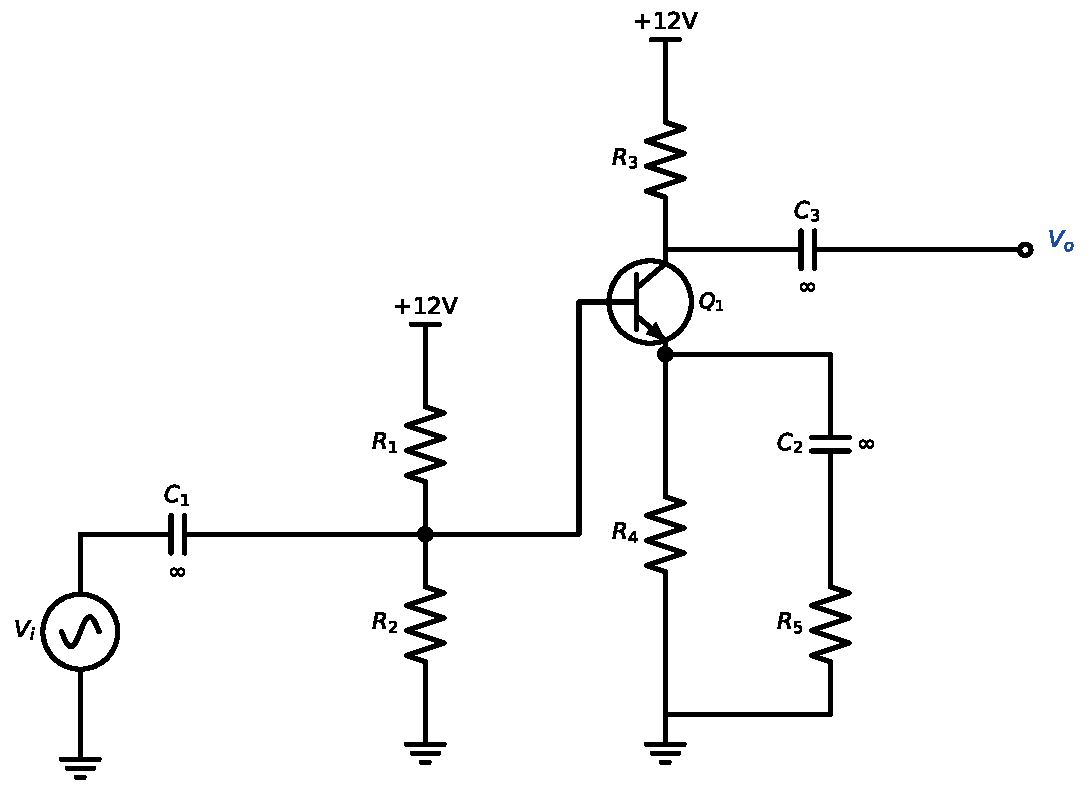
\includegraphics[width=\linewidth,height=6cm,keepaspectratio]{p01_circuit}\end{minipage}\hfill\begin{minipage}{0.38\linewidth}\begin{center}\small\renewcommand{\arraystretch}{1.35}
\begin{tabular}{ll}
\toprule
specification & value \\
\midrule
Supply voltage $V_{CC}$ & $12$\,V \\
0-to-peak output swing $\hat V_o$ & $\ge 2$\,V \\
Voltage gain $|A_v|$ & $50$ \\
Input resistance $R_i$ & $\ge 5\,\mathrm{k}\Omega$ \\
THD at $\hat V_o = 2$\,V & $\le 2\,\%$ \\
$\Delta I_C/I_C$ for $|V_{BE}| = 0.7\pm0.1$\,V & $\le 10\,\%$ \\
\bottomrule
\end{tabular}\end{center}
\end{minipage}
\end{probbox}

\begin{probbox}{Problem 4E.2 \hfill Easy}
Design the amplifier below (find all resistor values) for the specifications in the table, insensitive to $\beta$ and $V_{BE}$ variations. $\beta = 100$, $V_T = 25$\,mV, $|V_{BE}| = 0.7$\,V, $V_{CE,sat} = 0.2$\,V; capacitors marked $\infty$ are shorts at the signal frequency. Use: $N = 10$; $V_{RE1} = 1$\,V. Where a current is not given, take the nearest E12 value on the safe side.

\smallskip\noindent\begin{minipage}{0.6\linewidth}\centering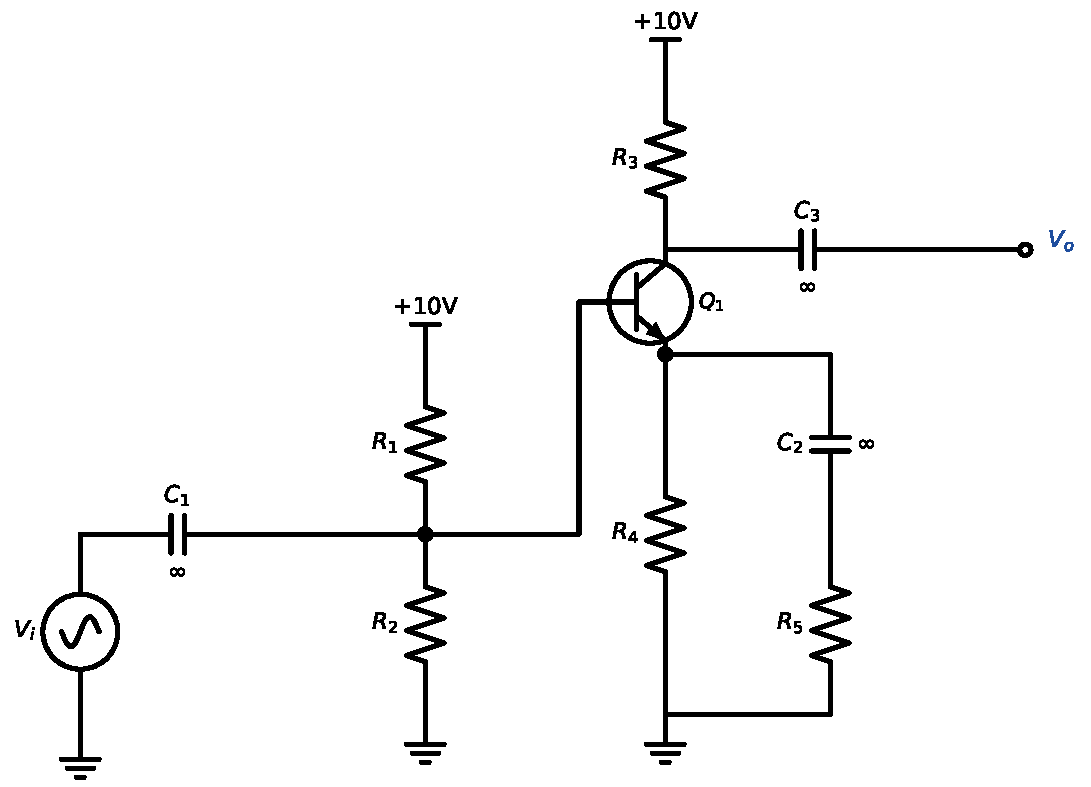
\includegraphics[width=\linewidth,height=6cm,keepaspectratio]{p02_circuit}\end{minipage}\hfill\begin{minipage}{0.38\linewidth}\begin{center}\small\renewcommand{\arraystretch}{1.35}
\begin{tabular}{ll}
\toprule
specification & value \\
\midrule
Supply voltage $V_{CC}$ & $10$\,V \\
0-to-peak output swing $\hat V_o$ & $\ge 1.5$\,V \\
Voltage gain $|A_v|$ & $80$ \\
Input resistance $R_i$ & $\ge 3\,\mathrm{k}\Omega$ \\
THD at $\hat V_o = 1.5$\,V & $\le 3\,\%$ \\
$\Delta I_C/I_C$ for $|V_{BE}| = 0.7\pm0.1$\,V & $\le 10\,\%$ \\
\bottomrule
\end{tabular}\end{center}
\end{minipage}
\end{probbox}

\begin{probbox}{Problem 4E.3 \hfill Easy}
Design the amplifier below (find all resistor values) for the specifications in the table, insensitive to $\beta$ and $V_{BE}$ variations. $\beta = 100$, $V_T = 25$\,mV, $|V_{BE}| = 0.7$\,V, $V_{CE,sat} = 0.2$\,V; capacitors marked $\infty$ are shorts at the signal frequency. Use: $N = 10$; $V_{RE1} = 1$\,V. Where a current is not given, take the nearest E12 value on the safe side.

\smallskip\noindent\begin{minipage}{0.6\linewidth}\centering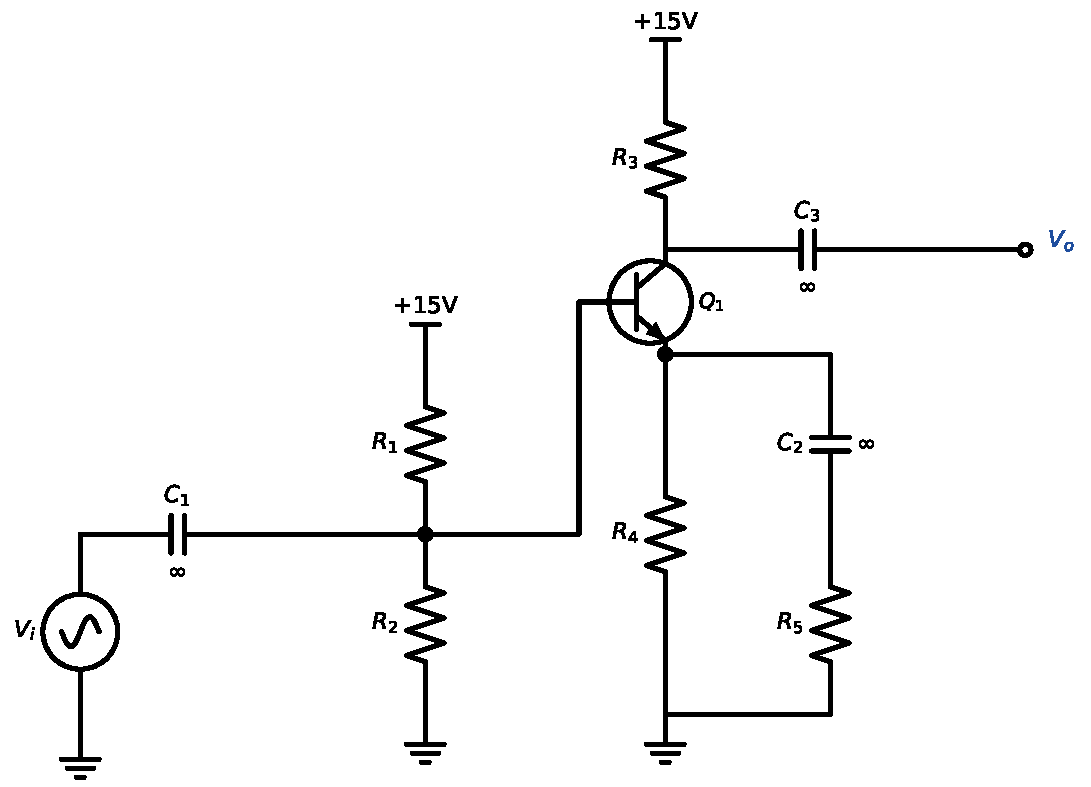
\includegraphics[width=\linewidth,height=6cm,keepaspectratio]{p03_circuit}\end{minipage}\hfill\begin{minipage}{0.38\linewidth}\begin{center}\small\renewcommand{\arraystretch}{1.35}
\begin{tabular}{ll}
\toprule
specification & value \\
\midrule
Supply voltage $V_{CC}$ & $15$\,V \\
0-to-peak output swing $\hat V_o$ & $\ge 3$\,V \\
Voltage gain $|A_v|$ & $30$ \\
Input resistance $R_i$ & $\ge 10\,\mathrm{k}\Omega$ \\
THD at $\hat V_o = 3$\,V & $\le 2\,\%$ \\
$\Delta I_C/I_C$ for $|V_{BE}| = 0.7\pm0.1$\,V & $\le 10\,\%$ \\
\bottomrule
\end{tabular}\end{center}
\end{minipage}
\end{probbox}

\begin{probbox}{Problem 4E.4 \hfill Easy}
Design the amplifier below (find all resistor values) for the specifications in the table, insensitive to $\beta$ and $V_{BE}$ variations. $\beta = 100$, $V_T = 25$\,mV, $|V_{BE}| = 0.7$\,V, $V_{CE,sat} = 0.2$\,V; capacitors marked $\infty$ are shorts at the signal frequency. Use: $N = 10$; $V_{RE1} = 1$\,V. Where a current is not given, take the nearest E12 value on the safe side.

\smallskip\noindent\begin{minipage}{0.6\linewidth}\centering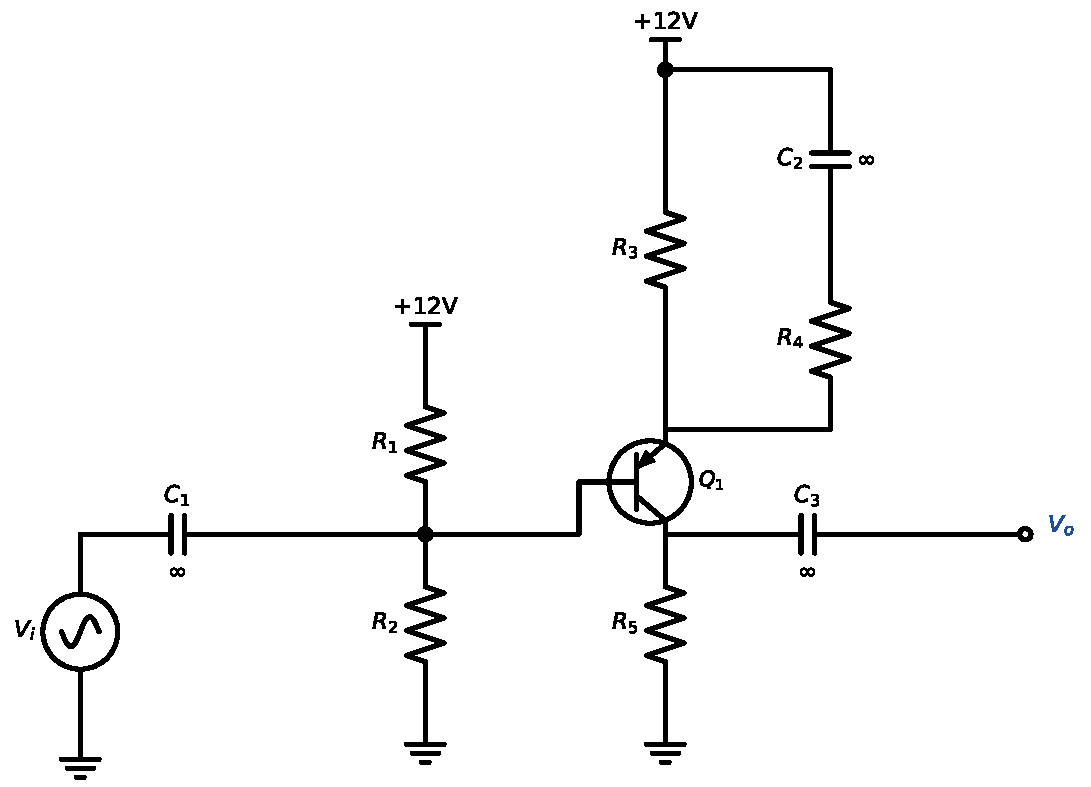
\includegraphics[width=\linewidth,height=6cm,keepaspectratio]{p04_circuit}\end{minipage}\hfill\begin{minipage}{0.38\linewidth}\begin{center}\small\renewcommand{\arraystretch}{1.35}
\begin{tabular}{ll}
\toprule
specification & value \\
\midrule
Supply voltage $V_{CC}$ & $12$\,V \\
0-to-peak output swing $\hat V_o$ & $\ge 2$\,V \\
Voltage gain $|A_v|$ & $40$ \\
Input resistance $R_i$ & $\ge 4\,\mathrm{k}\Omega$ \\
THD at $\hat V_o = 2$\,V & $\le 2\,\%$ \\
$\Delta I_C/I_C$ for $|V_{BE}| = 0.7\pm0.1$\,V & $\le 10\,\%$ \\
\bottomrule
\end{tabular}\end{center}
\end{minipage}
\end{probbox}

\begin{probbox}{Problem 4E.5 \hfill Easy}
Design the amplifier below (find all resistor values) for the specifications in the table, insensitive to $\beta$ and $V_{BE}$ variations. $\beta = 100$, $V_T = 25$\,mV, $|V_{BE}| = 0.7$\,V, $V_{CE,sat} = 0.2$\,V; capacitors marked $\infty$ are shorts at the signal frequency. Use: $N = 10$; $V_{RE1} = 1$\,V. Where a current is not given, take the nearest E12 value on the safe side.

\smallskip\noindent\begin{minipage}{0.6\linewidth}\centering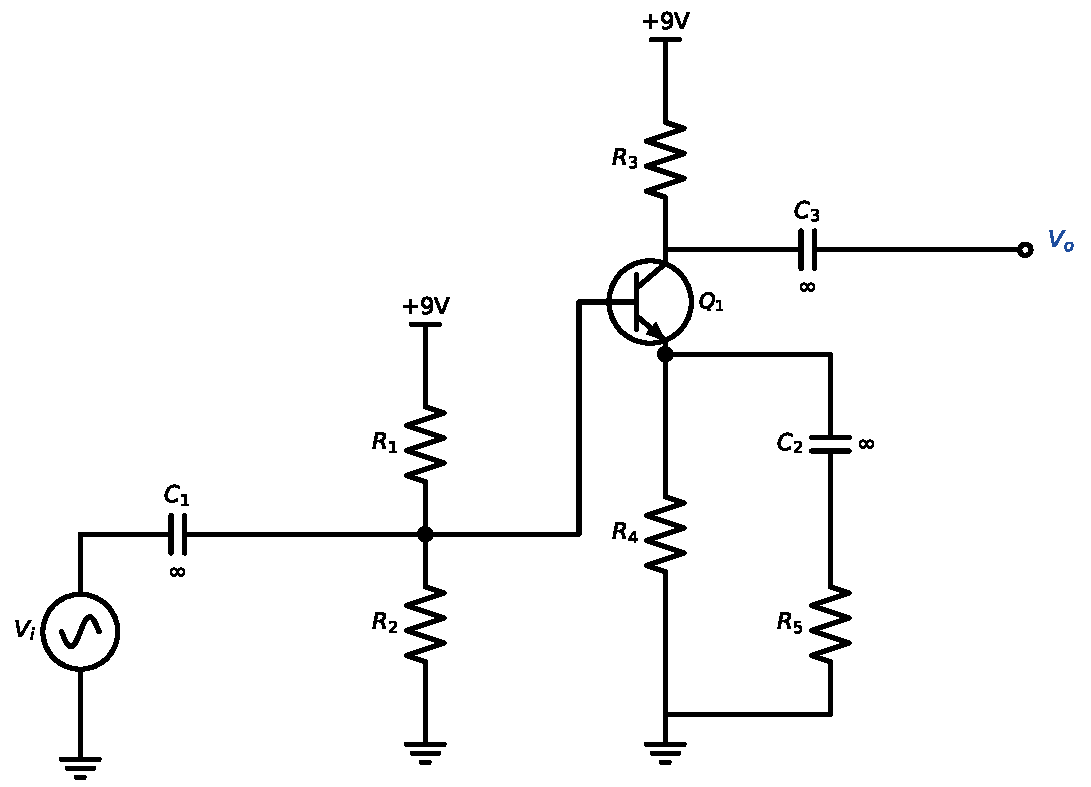
\includegraphics[width=\linewidth,height=6cm,keepaspectratio]{p05_circuit}\end{minipage}\hfill\begin{minipage}{0.38\linewidth}\begin{center}\small\renewcommand{\arraystretch}{1.35}
\begin{tabular}{ll}
\toprule
specification & value \\
\midrule
Supply voltage $V_{CC}$ & $9$\,V \\
0-to-peak output swing $\hat V_o$ & $\ge 1$\,V \\
Voltage gain $|A_v|$ & $100$ \\
Input resistance $R_i$ & $\ge 2\,\mathrm{k}\Omega$ \\
THD at $\hat V_o = 1$\,V & $\le 3\,\%$ \\
$\Delta I_C/I_C$ for $|V_{BE}| = 0.7\pm0.1$\,V & $\le 10\,\%$ \\
\bottomrule
\end{tabular}\end{center}
\end{minipage}
\end{probbox}

\begin{probbox}{Problem 4E.6 \hfill Easy}
Design the amplifier below (find all resistor values) for the specifications in the table, insensitive to $\beta$ and $V_{BE}$ variations. $\beta = 100$, $V_T = 25$\,mV, $|V_{BE}| = 0.7$\,V, $V_{CE,sat} = 0.2$\,V; capacitors marked $\infty$ are shorts at the signal frequency. Use: $N = 10$; $V_{RE1} = 1$\,V. Where a current is not given, take the nearest E12 value on the safe side.

\smallskip\noindent\begin{minipage}{0.6\linewidth}\centering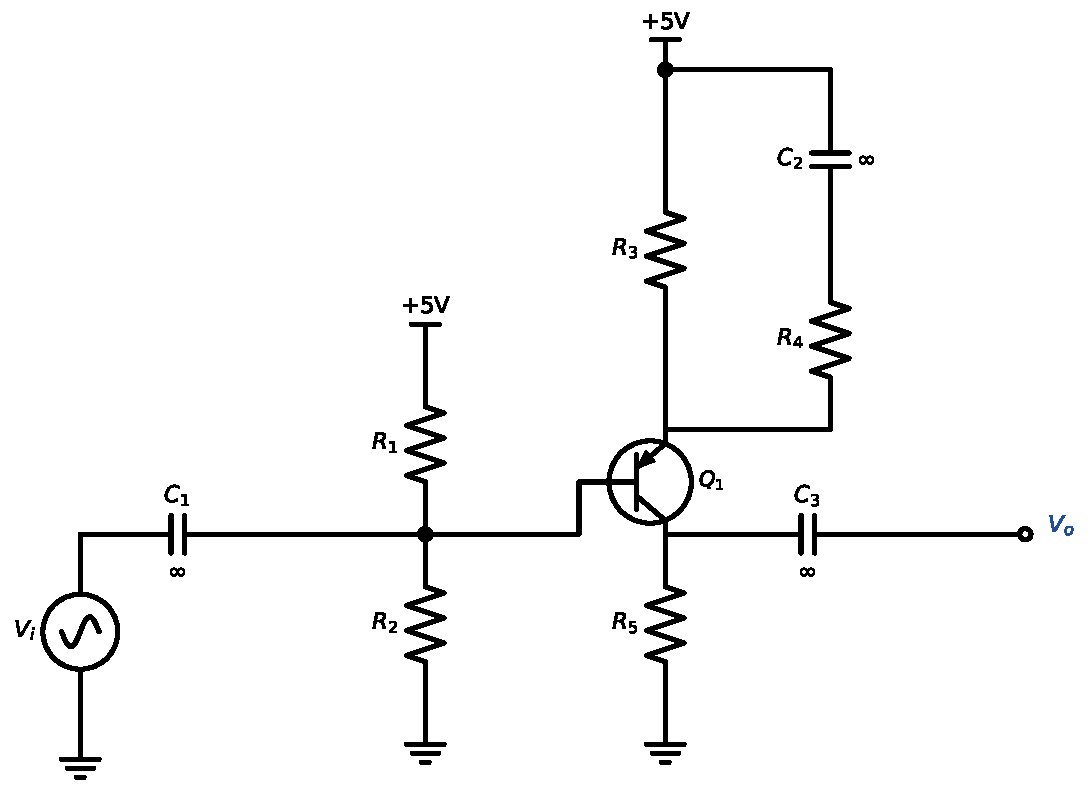
\includegraphics[width=\linewidth,height=6cm,keepaspectratio]{p06_circuit}\end{minipage}\hfill\begin{minipage}{0.38\linewidth}\begin{center}\small\renewcommand{\arraystretch}{1.35}
\begin{tabular}{ll}
\toprule
specification & value \\
\midrule
Supply voltage $V_{CC}$ & $5$\,V \\
0-to-peak output swing $\hat V_o$ & $\ge 1$\,V \\
Voltage gain $|A_v|$ & $50$ \\
Input resistance $R_i$ & $\ge 1\,\mathrm{k}\Omega$ \\
THD at $\hat V_o = 1$\,V & $\le 5\,\%$ \\
$\Delta I_C/I_C$ for $|V_{BE}| = 0.7\pm0.1$\,V & $\le 10\,\%$ \\
\bottomrule
\end{tabular}\end{center}
\end{minipage}
\end{probbox}

\subsection*{Medium problems}
\begin{probbox}{Problem 4E.7 \hfill Medium}
Design the amplifier below (find all resistor values) for the specifications in the table, insensitive to $\beta$ and $V_{BE}$ variations. $\beta = 100$, $V_T = 25$\,mV, $|V_{BE}| = 0.7$\,V, $V_{CE,sat} = 0.2$\,V; capacitors marked $\infty$ are shorts at the signal frequency. Use: $N = 10$; design for $\hat V_o = 1.8$\,V (margin); $V_{RE1} = 1$\,V. Where a current or $R_H$ is not given, take the nearest E12 value on the safe side.

\smallskip\noindent\begin{minipage}{0.6\linewidth}\centering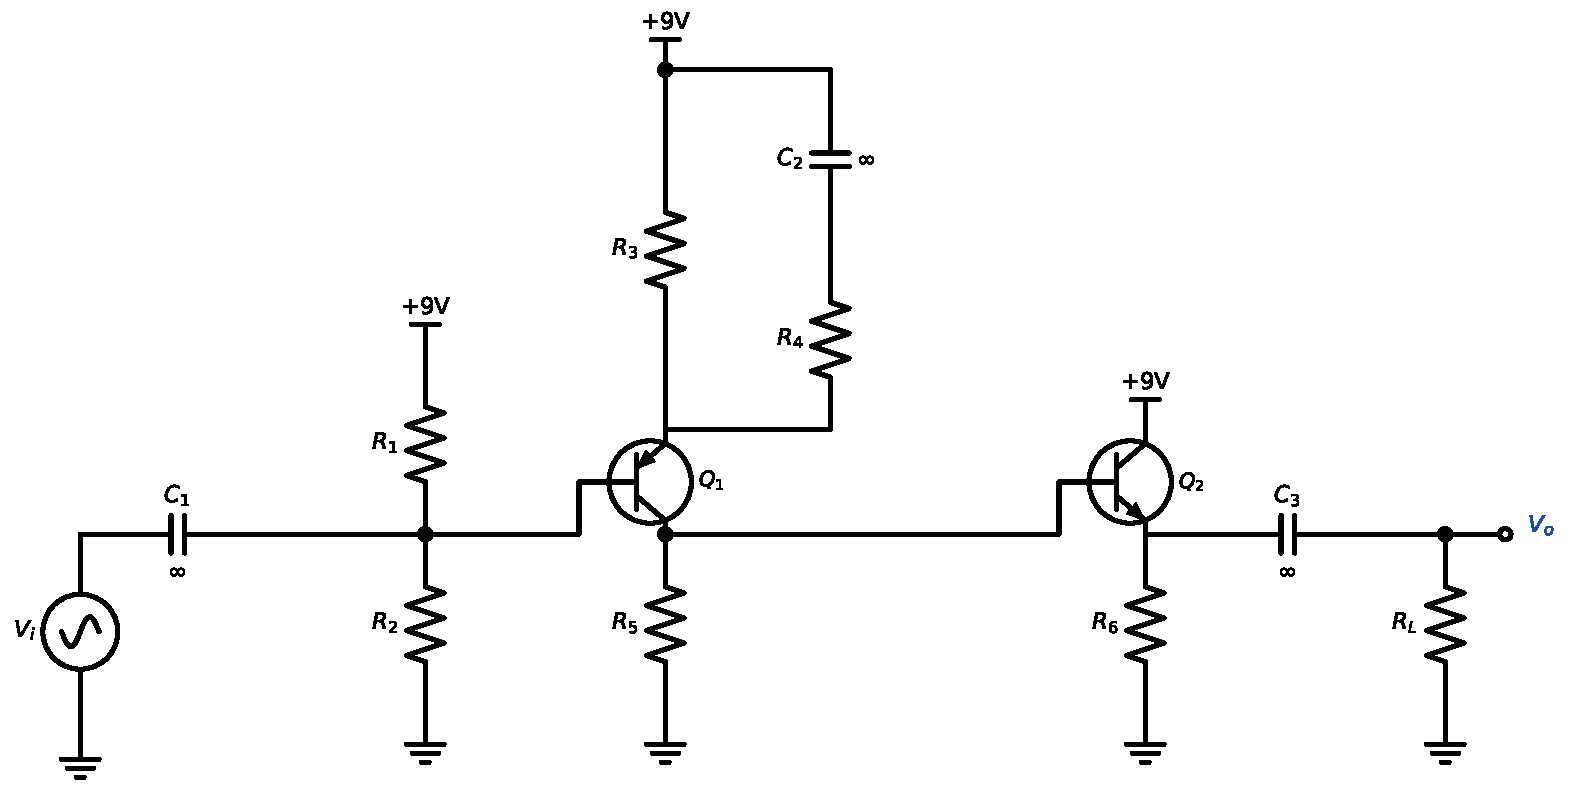
\includegraphics[width=\linewidth,height=6cm,keepaspectratio]{p07_circuit}\end{minipage}\hfill\begin{minipage}{0.38\linewidth}\begin{center}\small\renewcommand{\arraystretch}{1.35}
\begin{tabular}{ll}
\toprule
specification & value \\
\midrule
Supply voltage $V_{CC}$ & $9$\,V \\
0-to-peak output swing $\hat V_o$ & $\ge 1.5$\,V \\
Voltage gain $|A_v|$ & $40$ \\
Input resistance $R_i$ & $\ge 4\,\mathrm{k}\Omega$ \\
Load resistance $R_L$ & $500\,\Omega$ \\
THD at $\hat V_o = 1.5$\,V & $\le 3\,\%$ \\
$\Delta I_C/I_C$ for $|V_{BE}| = 0.7\pm0.1$\,V & $\le 10\,\%$ \\
\bottomrule
\end{tabular}\end{center}
\end{minipage}
\end{probbox}

\begin{probbox}{Problem 4E.8 \hfill Medium}
Design the amplifier below (find all resistor values) for the specifications in the table, insensitive to $\beta$ and $V_{BE}$ variations. $\beta = 100$, $V_T = 25$\,mV, $|V_{BE}| = 0.7$\,V, $V_{CE,sat} = 0.2$\,V; capacitors marked $\infty$ are shorts at the signal frequency. Use: $N = 10$; design for $\hat V_o = 2.4$\,V (margin); $V_{RE1} = 1$\,V. Where a current or $R_H$ is not given, take the nearest E12 value on the safe side.

\smallskip\noindent\begin{minipage}{0.6\linewidth}\centering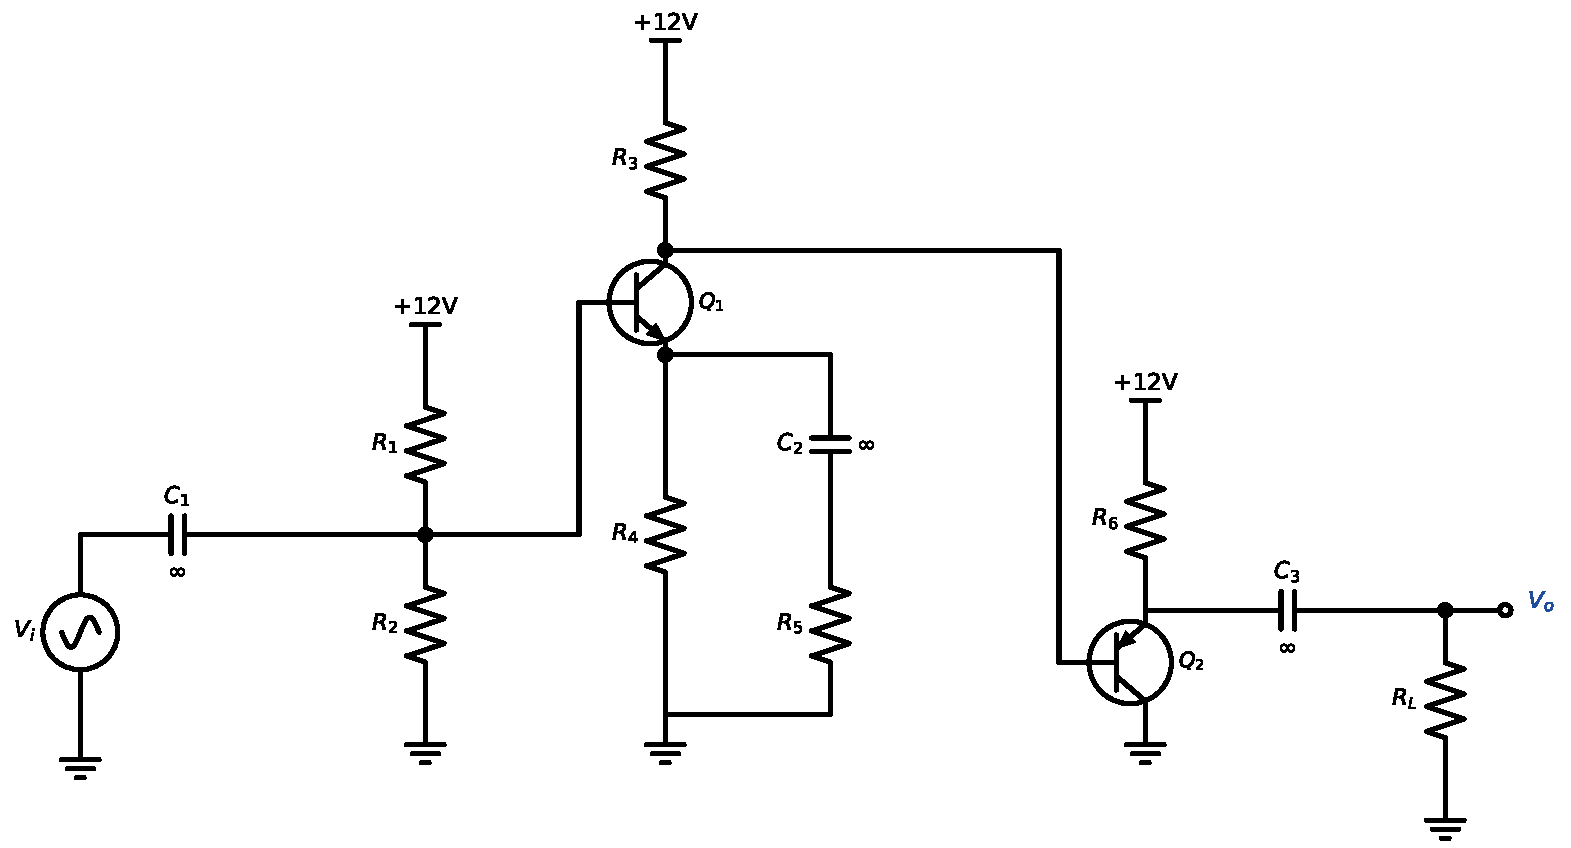
\includegraphics[width=\linewidth,height=6cm,keepaspectratio]{p08_circuit}\end{minipage}\hfill\begin{minipage}{0.38\linewidth}\begin{center}\small\renewcommand{\arraystretch}{1.35}
\begin{tabular}{ll}
\toprule
specification & value \\
\midrule
Supply voltage $V_{CC}$ & $12$\,V \\
0-to-peak output swing $\hat V_o$ & $\ge 2$\,V \\
Voltage gain $|A_v|$ & $60$ \\
Input resistance $R_i$ & $\ge 5\,\mathrm{k}\Omega$ \\
Load resistance $R_L$ & $1\,\mathrm{k}\Omega$ \\
THD at $\hat V_o = 2$\,V & $\le 3\,\%$ \\
$\Delta I_C/I_C$ for $|V_{BE}| = 0.7\pm0.1$\,V & $\le 10\,\%$ \\
\bottomrule
\end{tabular}\end{center}
\end{minipage}
\end{probbox}

\begin{probbox}{Problem 4E.9 \hfill Medium}
Design the amplifier below (find all resistor values) for the specifications in the table, insensitive to $\beta$ and $V_{BE}$ variations. $\beta = 100$, $V_T = 25$\,mV, $|V_{BE}| = 0.7$\,V, $V_{CE,sat} = 0.2$\,V; capacitors marked $\infty$ are shorts at the signal frequency. Use: $N = 10$; design for $\hat V_o = 1.2$\,V (margin); $V_{RE1} = 1$\,V. Where a current or $R_H$ is not given, take the nearest E12 value on the safe side.

\smallskip\noindent\begin{minipage}{0.6\linewidth}\centering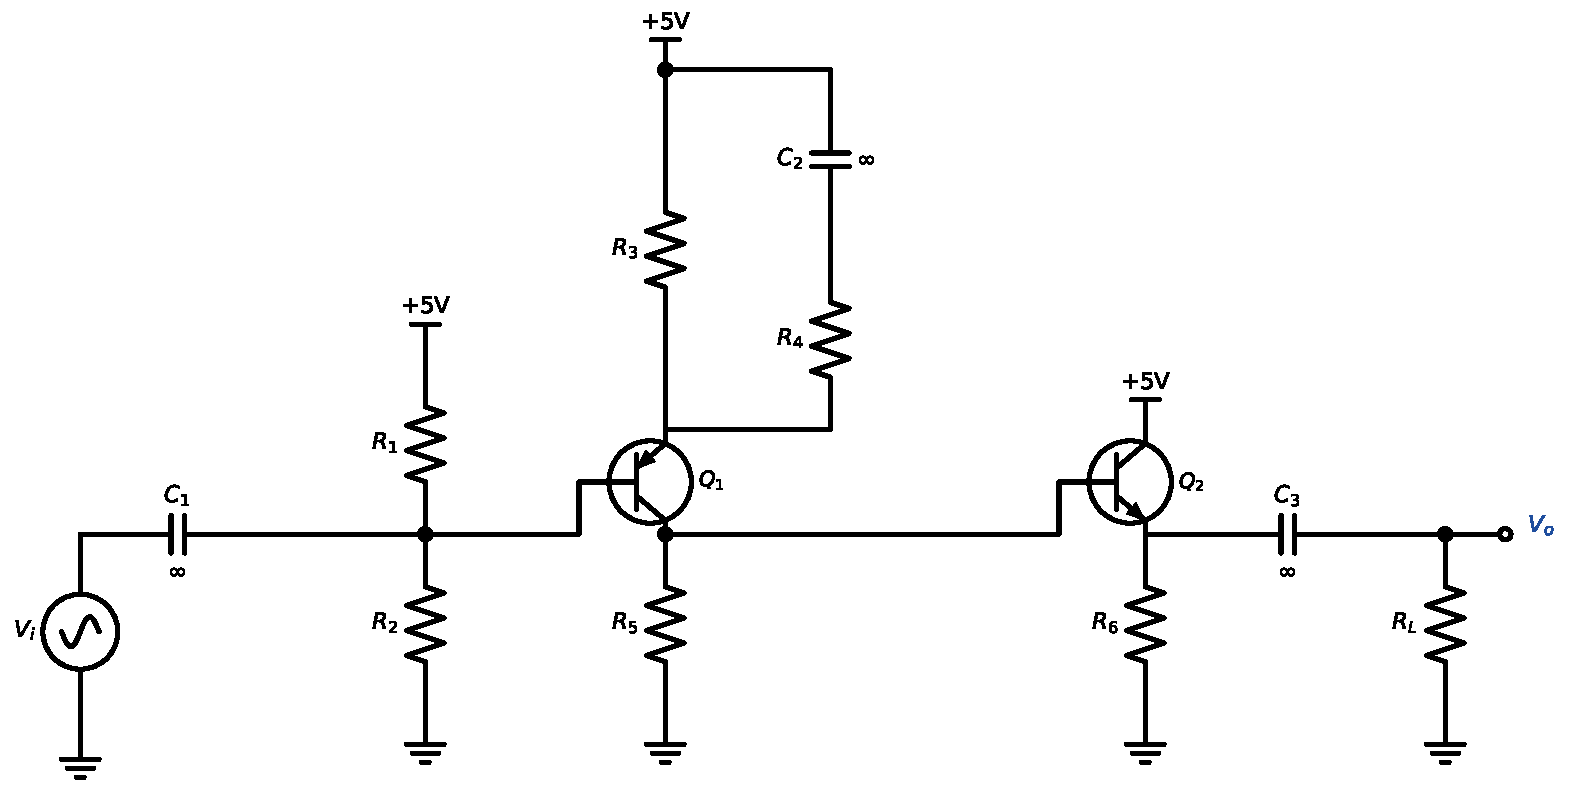
\includegraphics[width=\linewidth,height=6cm,keepaspectratio]{p09_circuit}\end{minipage}\hfill\begin{minipage}{0.38\linewidth}\begin{center}\small\renewcommand{\arraystretch}{1.35}
\begin{tabular}{ll}
\toprule
specification & value \\
\midrule
Supply voltage $V_{CC}$ & $5$\,V \\
0-to-peak output swing $\hat V_o$ & $\ge 1$\,V \\
Voltage gain $|A_v|$ & $30$ \\
Input resistance $R_i$ & $\ge 1.5\,\mathrm{k}\Omega$ \\
Load resistance $R_L$ & $200\,\Omega$ \\
THD at $\hat V_o = 1$\,V & $\le 5\,\%$ \\
$\Delta I_C/I_C$ for $|V_{BE}| = 0.7\pm0.1$\,V & $\le 10\,\%$ \\
\bottomrule
\end{tabular}\end{center}
\end{minipage}
\end{probbox}

\begin{probbox}{Problem 4E.10 \hfill Medium}
Design the amplifier below (find all resistor values) for the specifications in the table, insensitive to $\beta$ and $V_{BE}$ variations. $\beta = 100$, $V_T = 25$\,mV, $|V_{BE}| = 0.7$\,V, $V_{CE,sat} = 0.2$\,V; capacitors marked $\infty$ are shorts at the signal frequency. Use: $N = 10$; design for $\hat V_o = 1.8$\,V (margin); $V_{RE1} = 1$\,V. Where a current or $R_H$ is not given, take the nearest E12 value on the safe side.

\smallskip\noindent\begin{minipage}{0.6\linewidth}\centering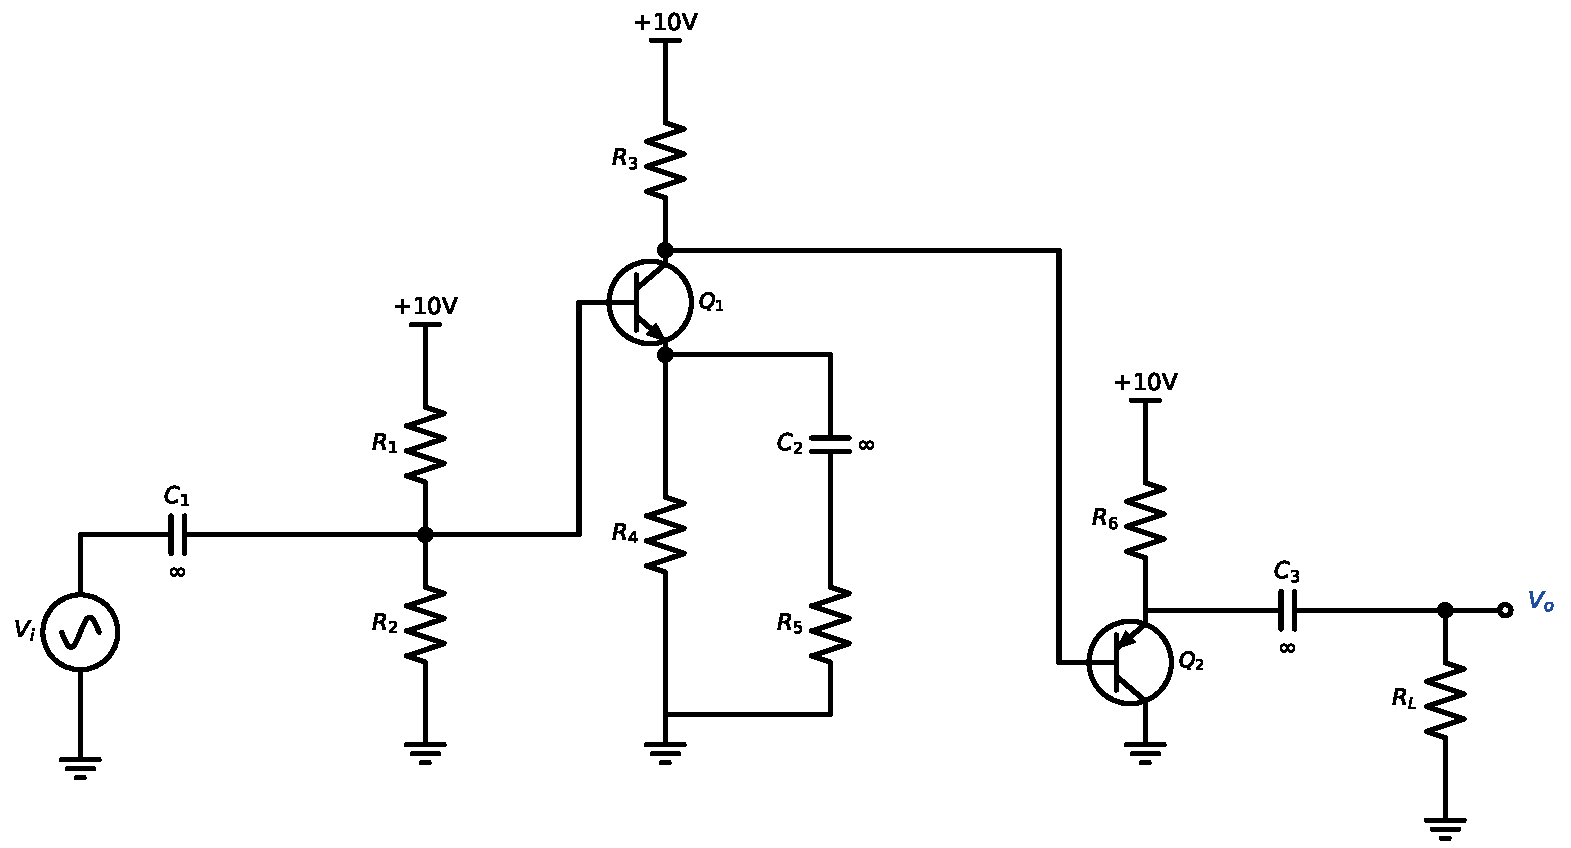
\includegraphics[width=\linewidth,height=6cm,keepaspectratio]{p10_circuit}\end{minipage}\hfill\begin{minipage}{0.38\linewidth}\begin{center}\small\renewcommand{\arraystretch}{1.35}
\begin{tabular}{ll}
\toprule
specification & value \\
\midrule
Supply voltage $V_{CC}$ & $10$\,V \\
0-to-peak output swing $\hat V_o$ & $\ge 1.5$\,V \\
Voltage gain $|A_v|$ & $100$ \\
Input resistance $R_i$ & $\ge 3\,\mathrm{k}\Omega$ \\
Load resistance $R_L$ & $300\,\Omega$ \\
THD at $\hat V_o = 1.5$\,V & $\le 5\,\%$ \\
$\Delta I_C/I_C$ for $|V_{BE}| = 0.7\pm0.1$\,V & $\le 10\,\%$ \\
\bottomrule
\end{tabular}\end{center}
\end{minipage}
\end{probbox}

\begin{probbox}{Problem 4E.11 \hfill Medium}
Design the amplifier below (find all resistor values) for the specifications in the table, insensitive to $\beta$ and $V_{BE}$ variations. $\beta = 100$, $V_T = 25$\,mV, $|V_{BE}| = 0.7$\,V, $V_{CE,sat} = 0.2$\,V; capacitors marked $\infty$ are shorts at the signal frequency. Use: $N = 20$; design for $\hat V_o = 3.5$\,V (margin); $V_{RE1} = 1$\,V. Where a current or $R_H$ is not given, take the nearest E12 value on the safe side.

\smallskip\noindent\begin{minipage}{0.6\linewidth}\centering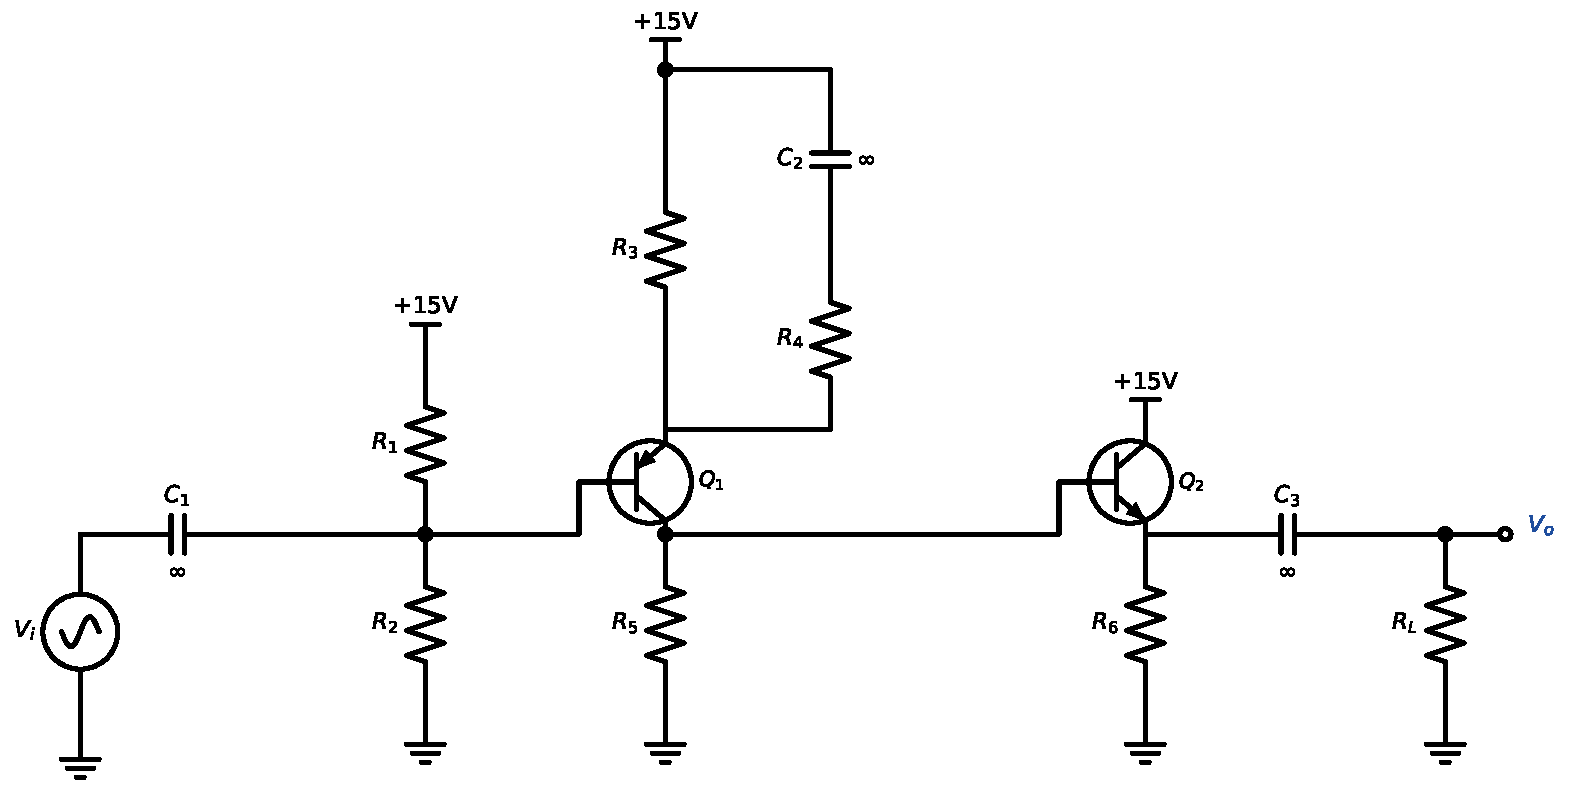
\includegraphics[width=\linewidth,height=6cm,keepaspectratio]{p11_circuit}\end{minipage}\hfill\begin{minipage}{0.38\linewidth}\begin{center}\small\renewcommand{\arraystretch}{1.35}
\begin{tabular}{ll}
\toprule
specification & value \\
\midrule
Supply voltage $V_{CC}$ & $15$\,V \\
0-to-peak output swing $\hat V_o$ & $\ge 3$\,V \\
Voltage gain $|A_v|$ & $30$ \\
Input resistance $R_i$ & $\ge 10\,\mathrm{k}\Omega$ \\
Load resistance $R_L$ & $1\,\mathrm{k}\Omega$ \\
THD at $\hat V_o = 3$\,V & $\le 3\,\%$ \\
$\Delta I_C/I_C$ for $|V_{BE}| = 0.7\pm0.1$\,V & $\le 10\,\%$ \\
\bottomrule
\end{tabular}\end{center}
\end{minipage}
\end{probbox}

\begin{probbox}{Problem 4E.12 \hfill Medium}
Design the amplifier below (find all resistor values) for the specifications in the table, insensitive to $\beta$ and $V_{BE}$ variations. $\beta = 100$, $V_T = 25$\,mV, $|V_{BE}| = 0.7$\,V, $V_{CE,sat} = 0.2$\,V; capacitors marked $\infty$ are shorts at the signal frequency. Use: $N = 10$; design for $\hat V_o = 1.2$\,V (margin); $V_{RE1} = 1$\,V. Where a current or $R_H$ is not given, take the nearest E12 value on the safe side.

\smallskip\noindent\begin{minipage}{0.6\linewidth}\centering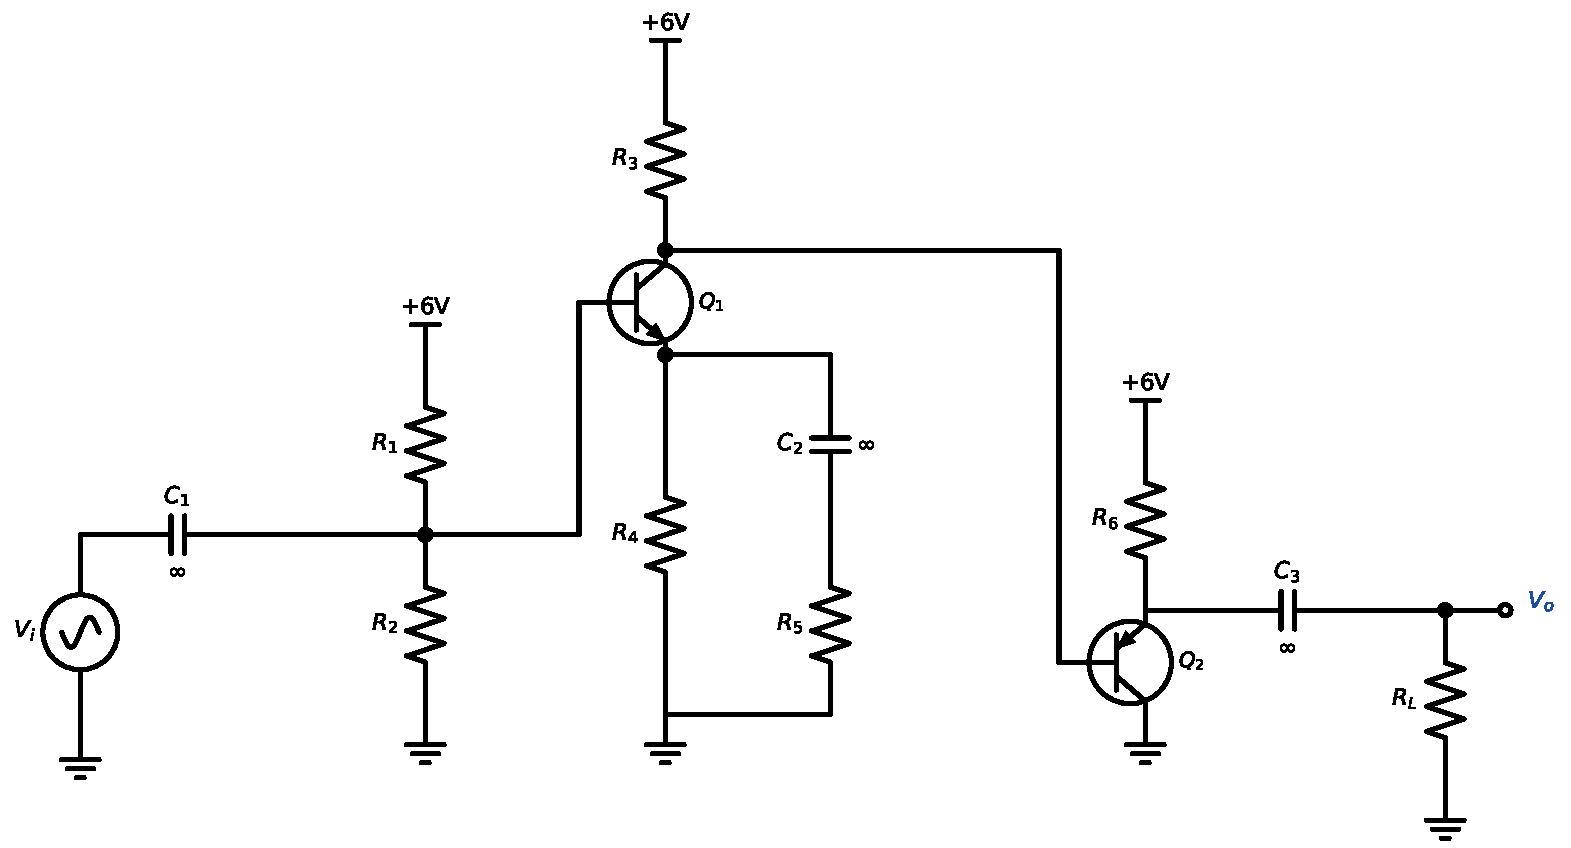
\includegraphics[width=\linewidth,height=6cm,keepaspectratio]{p12_circuit}\end{minipage}\hfill\begin{minipage}{0.38\linewidth}\begin{center}\small\renewcommand{\arraystretch}{1.35}
\begin{tabular}{ll}
\toprule
specification & value \\
\midrule
Supply voltage $V_{CC}$ & $6$\,V \\
0-to-peak output swing $\hat V_o$ & $\ge 1$\,V \\
Voltage gain $|A_v|$ & $25$ \\
Input resistance $R_i$ & $\ge 2\,\mathrm{k}\Omega$ \\
Load resistance $R_L$ & $100\,\Omega$ \\
THD at $\hat V_o = 1$\,V & $\le 3\,\%$ \\
$\Delta I_C/I_C$ for $|V_{BE}| = 0.7\pm0.1$\,V & $\le 10\,\%$ \\
\bottomrule
\end{tabular}\end{center}
\end{minipage}
\end{probbox}

\subsection*{Hard problems}
\begin{probbox}{Problem 4E.13 \hfill Hard}
Design the amplifier below (find all resistor values) for the specifications in the table, insensitive to $\beta$ and $V_{BE}$ variations. $\beta = 100$, $V_T = 25$\,mV, $|V_{BE}| = 0.7$\,V, $V_{CE,sat} = 0.2$\,V; capacitors marked $\infty$ are shorts at the signal frequency. Use: $N = 20$; design for $\hat V_o = 1.3$\,V (margin); $V_{RE1} = 1.8$\,V, $V_{RE2} = 1$\,V; $|A_{v2}| = 6$; $I_{C2} = 8\,\mathrm{m}\mathrm{A}$; $R_H = 50\,\Omega$. Where a current or $R_H$ is not given, take the nearest E12 value on the safe side. (These are the specifications of Sample Problem 11.)\begin{center}\small\renewcommand{\arraystretch}{1.35}
\begin{tabular}{ll}
\toprule
specification & value \\
\midrule
Supply voltage $V_{CC}$ & $5$\,V \\
0-to-peak output swing $\hat V_o$ & $\ge 1$\,V \\
Voltage gain $|A_v|$ & $100$ \\
Input resistance $R_i$ & $\ge 2\,\mathrm{k}\Omega$ \\
Load resistance $R_L$ & $150\,\Omega$ \\
THD at $\hat V_o = 1$\,V & $\le 3\,\%$ \\
$\Delta I_C/I_C$ for $|V_{BE}| = 0.7\pm0.1$\,V & $\le 10\,\%$ \\
\bottomrule
\end{tabular}\end{center}

\begin{center}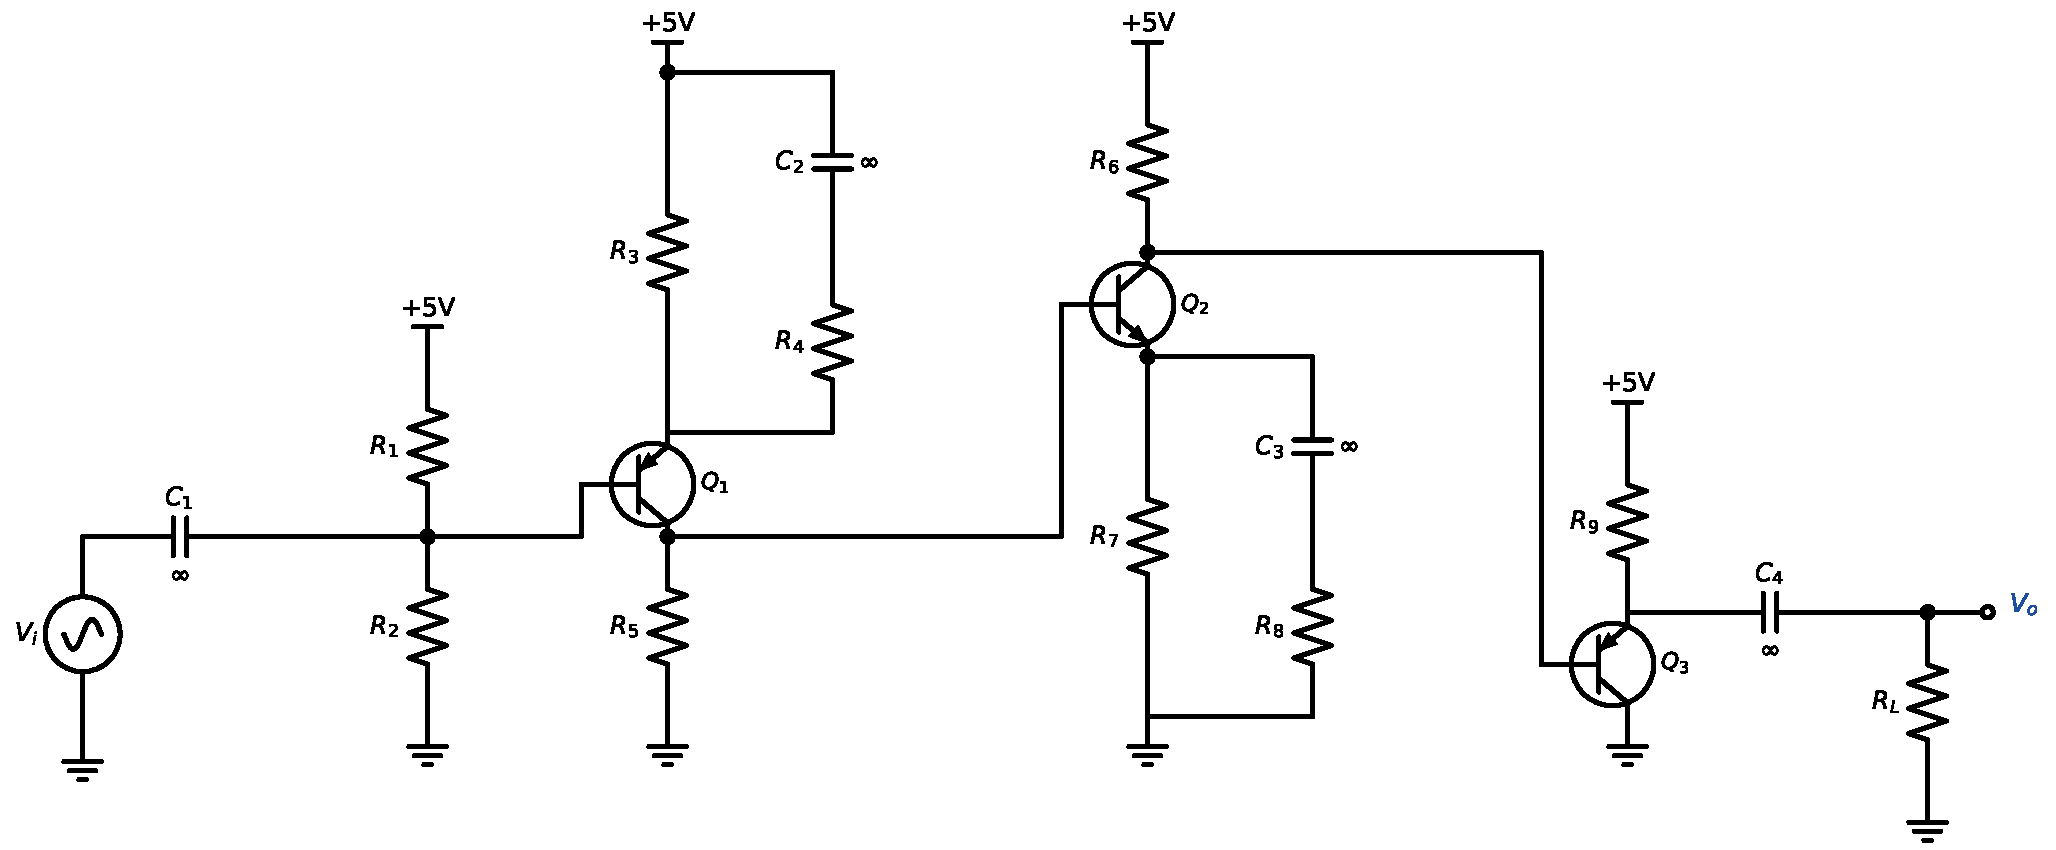
\includegraphics[width=\linewidth,height=6cm,keepaspectratio]{p13_circuit}\end{center}
\end{probbox}

\begin{probbox}{Problem 4E.14 \hfill Hard}
Design the amplifier below (find all resistor values) for the specifications in the table, insensitive to $\beta$ and $V_{BE}$ variations. $\beta = 100$, $V_T = 25$\,mV, $|V_{BE}| = 0.7$\,V, $V_{CE,sat} = 0.2$\,V; capacitors marked $\infty$ are shorts at the signal frequency. Use: $N = 10$; design for $\hat V_o = 2.4$\,V (margin); $V_{RE1} = 1$\,V, $V_{RE2} = 1$\,V; $|A_{v2}| = 10$. Where a current or $R_H$ is not given, take the nearest E12 value on the safe side.\begin{center}\small\renewcommand{\arraystretch}{1.35}
\begin{tabular}{ll}
\toprule
specification & value \\
\midrule
Supply voltage $V_{CC}$ & $10$\,V \\
0-to-peak output swing $\hat V_o$ & $\ge 2$\,V \\
Voltage gain $|A_v|$ & $200$ \\
Input resistance $R_i$ & $\ge 5\,\mathrm{k}\Omega$ \\
Load resistance $R_L$ & $500\,\Omega$ \\
THD at $\hat V_o = 2$\,V & $\le 5\,\%$ \\
$\Delta I_C/I_C$ for $|V_{BE}| = 0.7\pm0.1$\,V & $\le 10\,\%$ \\
\bottomrule
\end{tabular}\end{center}

\begin{center}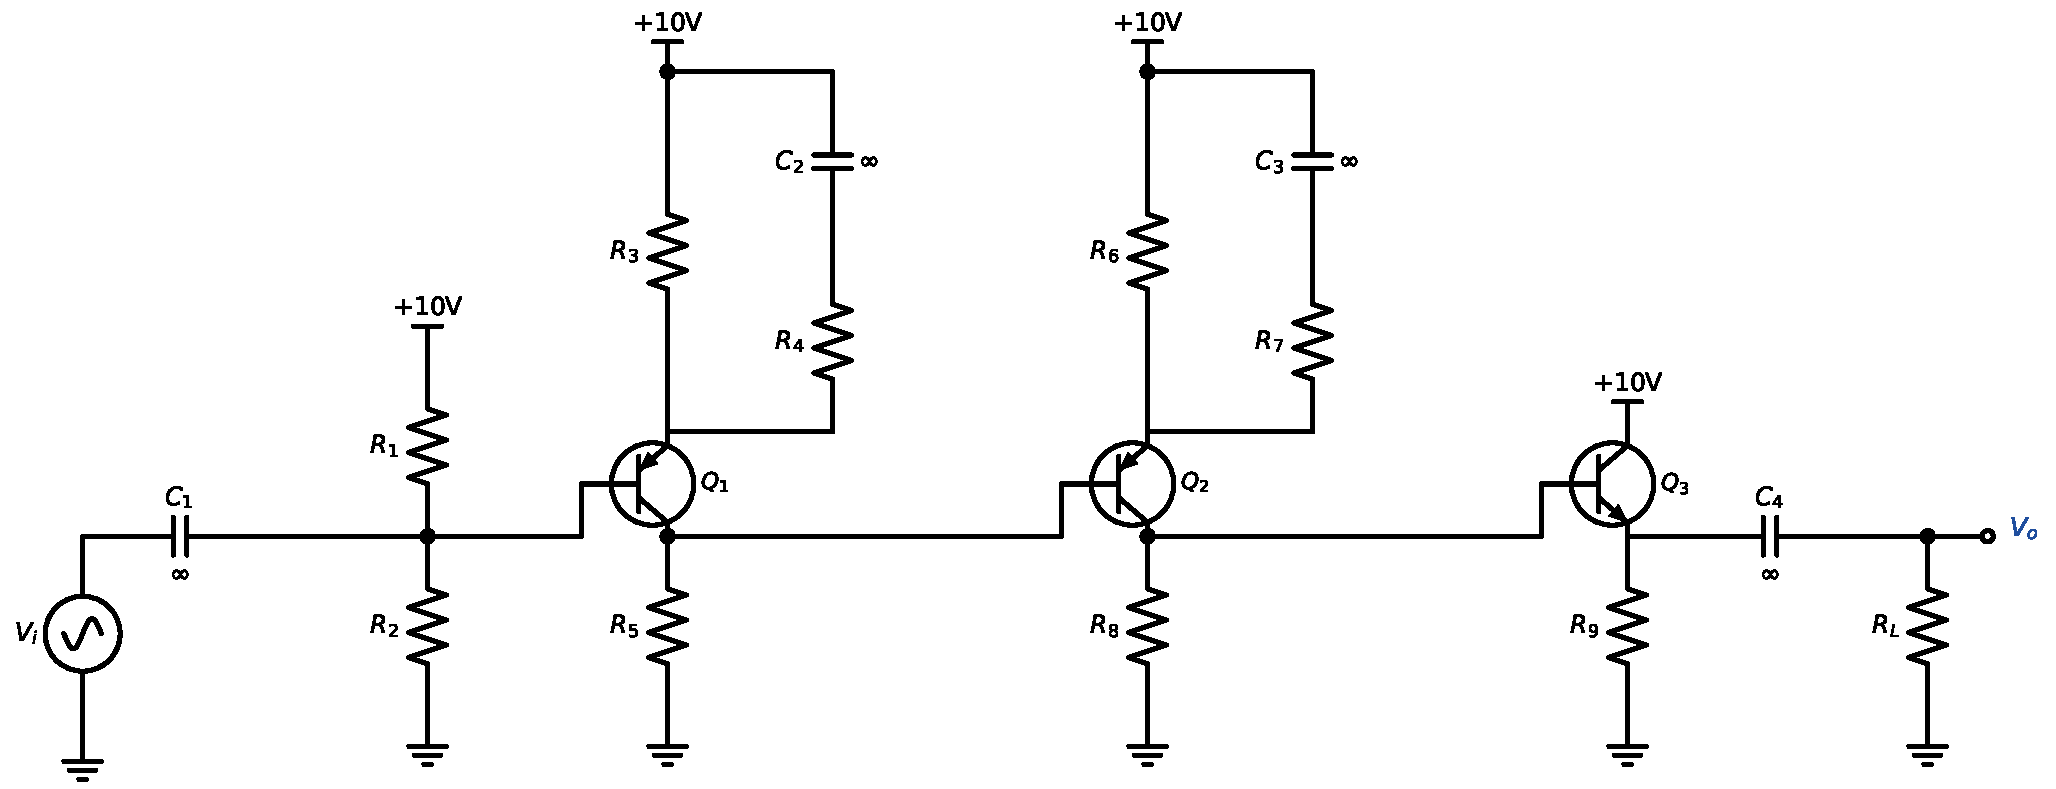
\includegraphics[width=\linewidth,height=6cm,keepaspectratio]{p14_circuit}\end{center}
\end{probbox}

\begin{probbox}{Problem 4E.15 \hfill Hard}
Design the amplifier below (find all resistor values) for the specifications in the table, insensitive to $\beta$ and $V_{BE}$ variations. $\beta = 100$, $V_T = 25$\,mV, $|V_{BE}| = 0.7$\,V, $V_{CE,sat} = 0.2$\,V; capacitors marked $\infty$ are shorts at the signal frequency. Use: $N = 20$; design for $\hat V_o = 2.4$\,V (margin); $V_{RE1} = 1.5$\,V, $V_{RE2} = 1$\,V; $|A_{v2}| = 8$. Where a current or $R_H$ is not given, take the nearest E12 value on the safe side.\begin{center}\small\renewcommand{\arraystretch}{1.35}
\begin{tabular}{ll}
\toprule
specification & value \\
\midrule
Supply voltage $V_{CC}$ & $12$\,V \\
0-to-peak output swing $\hat V_o$ & $\ge 2$\,V \\
Voltage gain $|A_v|$ & $150$ \\
Input resistance $R_i$ & $\ge 4\,\mathrm{k}\Omega$ \\
Load resistance $R_L$ & $1\,\mathrm{k}\Omega$ \\
THD at $\hat V_o = 2$\,V & $\le 5\,\%$ \\
$\Delta I_C/I_C$ for $|V_{BE}| = 0.7\pm0.1$\,V & $\le 10\,\%$ \\
\bottomrule
\end{tabular}\end{center}

\begin{center}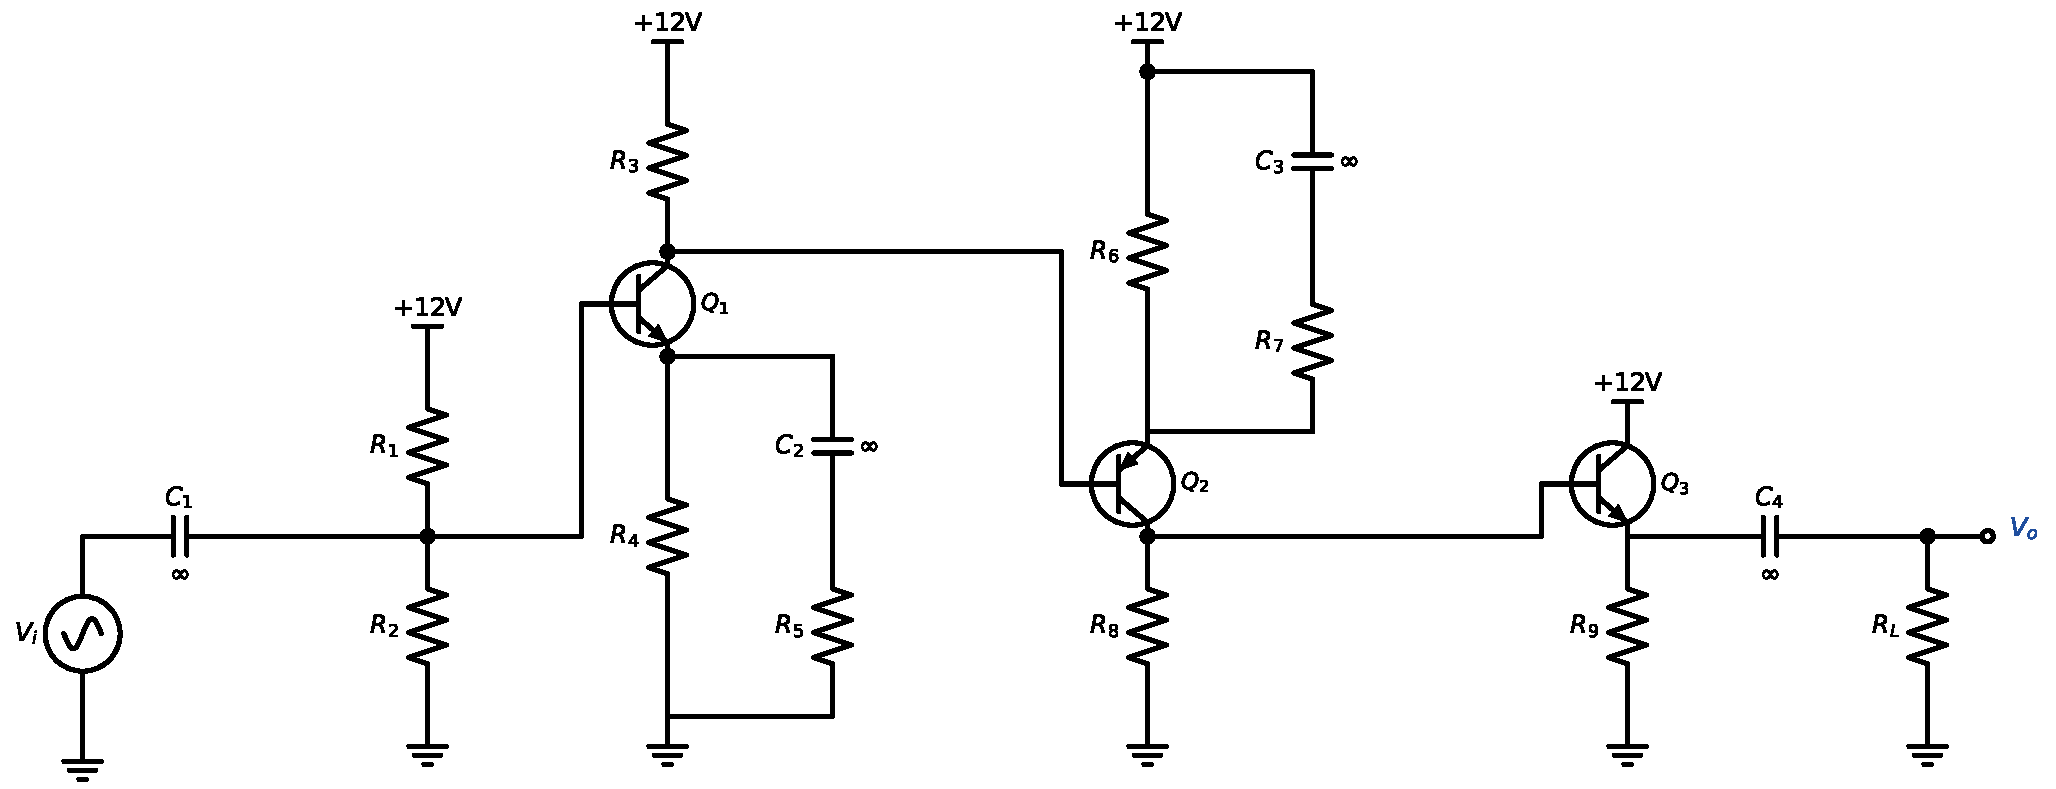
\includegraphics[width=\linewidth,height=6cm,keepaspectratio]{p15_circuit}\end{center}
\end{probbox}

\begin{probbox}{Problem 4E.16 \hfill Hard}
Design the amplifier below (find all resistor values) for the specifications in the table, insensitive to $\beta$ and $V_{BE}$ variations. $\beta = 100$, $V_T = 25$\,mV, $|V_{BE}| = 0.7$\,V, $V_{CE,sat} = 0.2$\,V; capacitors marked $\infty$ are shorts at the signal frequency. Use: $N = 10$; design for $\hat V_o = 1.8$\,V (margin); $V_{RE1} = 1$\,V, $V_{RE2} = 1$\,V; $|A_{v2}| = 8$. Where a current or $R_H$ is not given, take the nearest E12 value on the safe side.\begin{center}\small\renewcommand{\arraystretch}{1.35}
\begin{tabular}{ll}
\toprule
specification & value \\
\midrule
Supply voltage $V_{CC}$ & $9$\,V \\
0-to-peak output swing $\hat V_o$ & $\ge 1.5$\,V \\
Voltage gain $|A_v|$ & $120$ \\
Input resistance $R_i$ & $\ge 3\,\mathrm{k}\Omega$ \\
Load resistance $R_L$ & $300\,\Omega$ \\
THD at $\hat V_o = 1.5$\,V & $\le 5\,\%$ \\
$\Delta I_C/I_C$ for $|V_{BE}| = 0.7\pm0.1$\,V & $\le 10\,\%$ \\
\bottomrule
\end{tabular}\end{center}

\begin{center}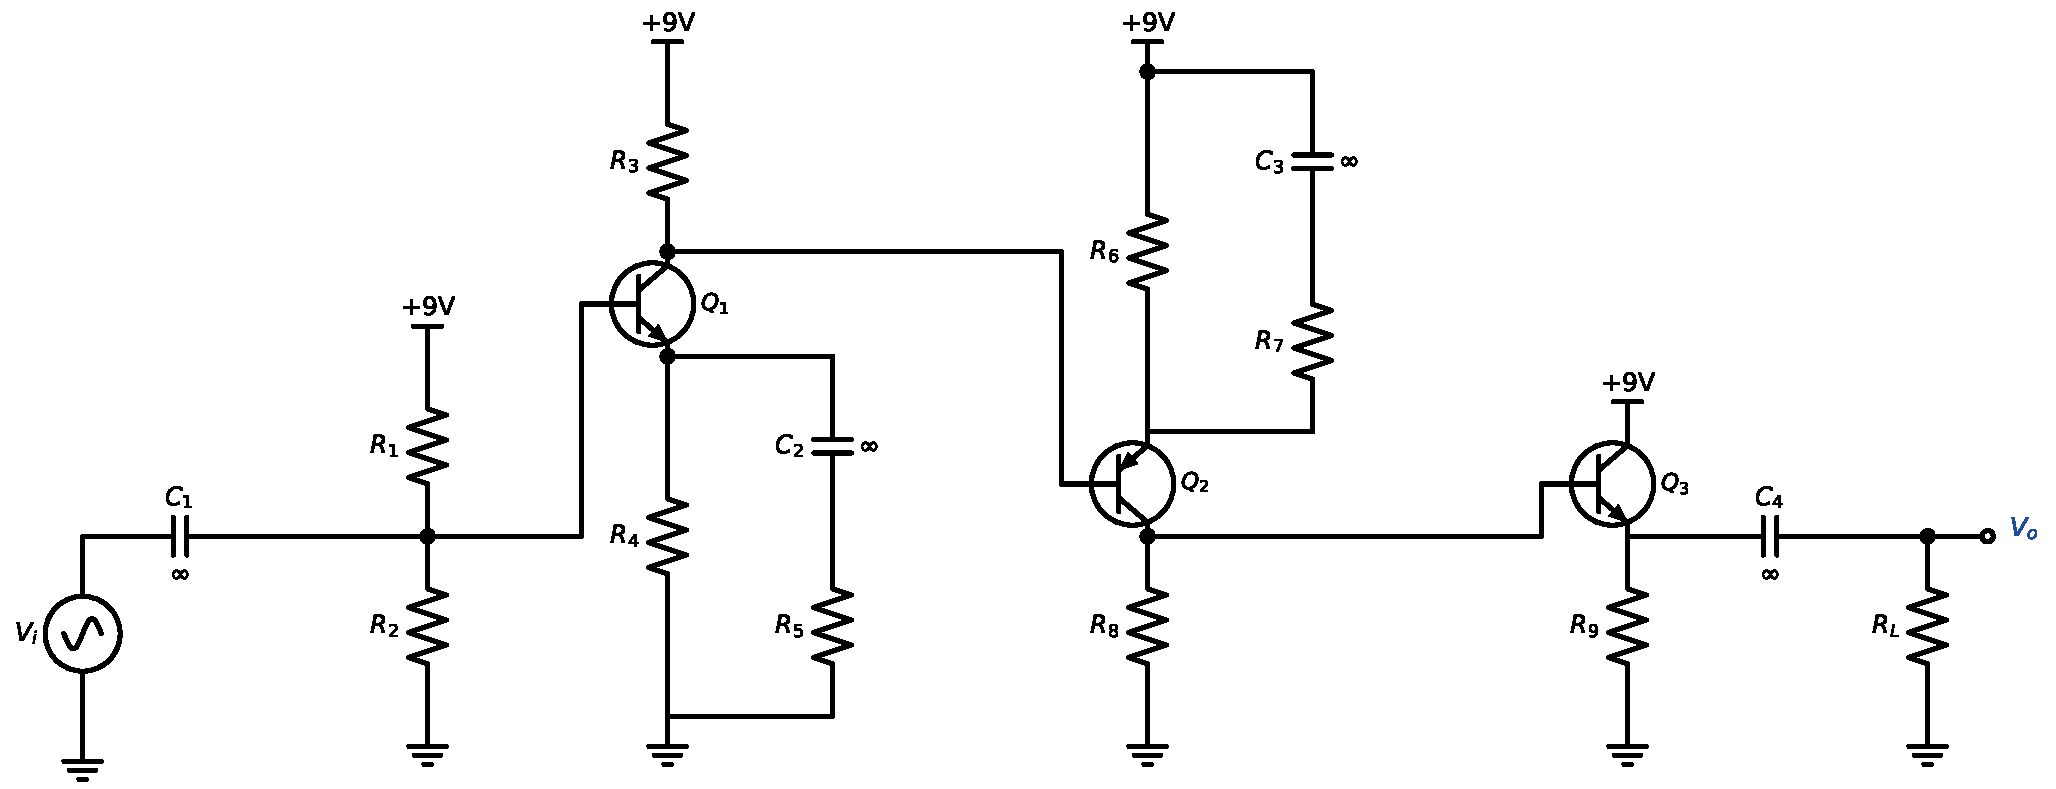
\includegraphics[width=\linewidth,height=6cm,keepaspectratio]{p16_circuit}\end{center}
\end{probbox}

\begin{probbox}{Problem 4E.17 \hfill Hard}
Design the amplifier below (find all resistor values) for the specifications in the table, insensitive to $\beta$ and $V_{BE}$ variations. $\beta = 100$, $V_T = 25$\,mV, $|V_{BE}| = 0.7$\,V, $V_{CE,sat} = 0.2$\,V; capacitors marked $\infty$ are shorts at the signal frequency. Use: $N = 20$; design for $\hat V_o = 2.5$\,V (margin); $V_{RE1} = 1.5$\,V, $V_{RE2} = 1$\,V; $|A_{v2}| = 8$. Where a current or $R_H$ is not given, take the nearest E12 value on the safe side.\begin{center}\small\renewcommand{\arraystretch}{1.35}
\begin{tabular}{ll}
\toprule
specification & value \\
\midrule
Supply voltage $V_{CC}$ & $9$\,V \\
0-to-peak output swing $\hat V_o$ & $\ge 2$\,V \\
Voltage gain $|A_v|$ & $150$ \\
Input resistance $R_i$ & $\ge 2\,\mathrm{k}\Omega$ \\
Load resistance $R_L$ & $200\,\Omega$ \\
THD at $\hat V_o = 2$\,V & $\le 5\,\%$ \\
$\Delta I_C/I_C$ for $|V_{BE}| = 0.7\pm0.1$\,V & $\le 10\,\%$ \\
\bottomrule
\end{tabular}\end{center}

\begin{center}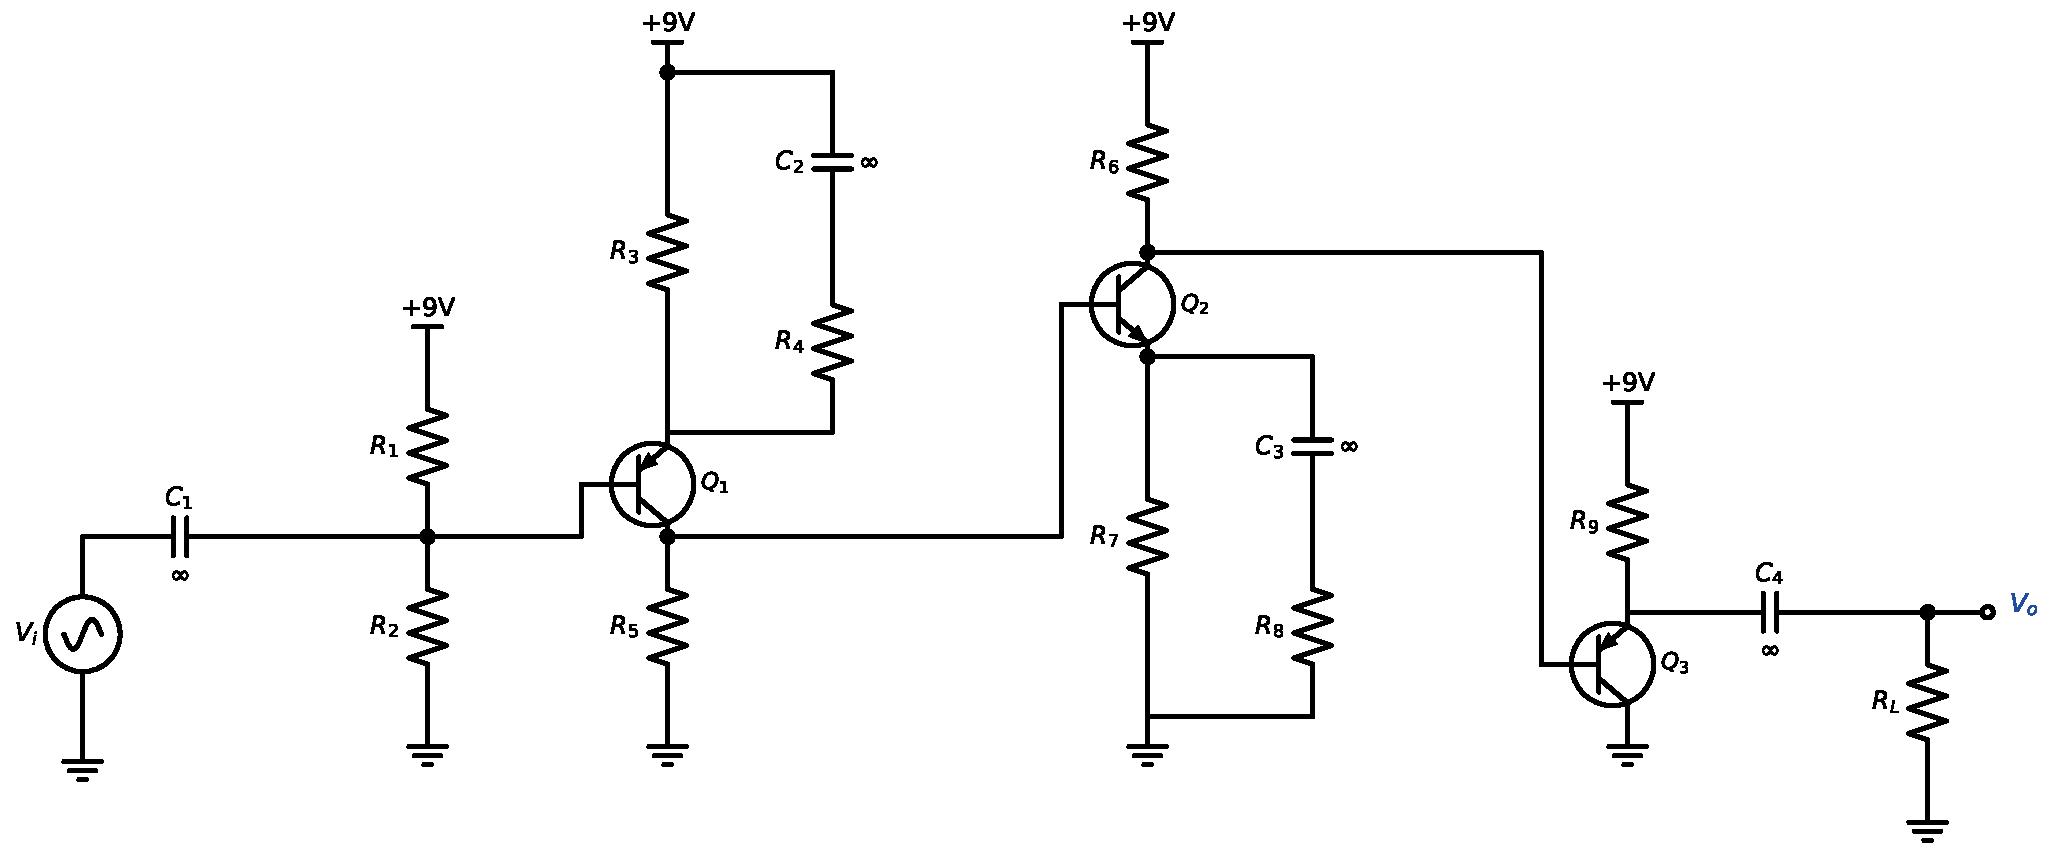
\includegraphics[width=\linewidth,height=6cm,keepaspectratio]{p17_circuit}\end{center}
\end{probbox}

\begin{probbox}{Problem 4E.18 \hfill Hard}
Design the amplifier below (find all resistor values) for the specifications in the table, insensitive to $\beta$ and $V_{BE}$ variations. $\beta = 100$, $V_T = 25$\,mV, $|V_{BE}| = 0.7$\,V, $V_{CE,sat} = 0.2$\,V; capacitors marked $\infty$ are shorts at the signal frequency. Use: $N = 10$; design for $\hat V_o = 3.5$\,V (margin); $V_{RE1} = 1$\,V, $V_{RE2} = 1$\,V; $|A_{v2}| = 12$. Where a current or $R_H$ is not given, take the nearest E12 value on the safe side.\begin{center}\small\renewcommand{\arraystretch}{1.35}
\begin{tabular}{ll}
\toprule
specification & value \\
\midrule
Supply voltage $V_{CC}$ & $12$\,V \\
0-to-peak output swing $\hat V_o$ & $\ge 3$\,V \\
Voltage gain $|A_v|$ & $300$ \\
Input resistance $R_i$ & $\ge 2\,\mathrm{k}\Omega$ \\
Load resistance $R_L$ & $1\,\mathrm{k}\Omega$ \\
THD at $\hat V_o = 3$\,V & $\le 5\,\%$ \\
$\Delta I_C/I_C$ for $|V_{BE}| = 0.7\pm0.1$\,V & $\le 10\,\%$ \\
\bottomrule
\end{tabular}\end{center}

\begin{center}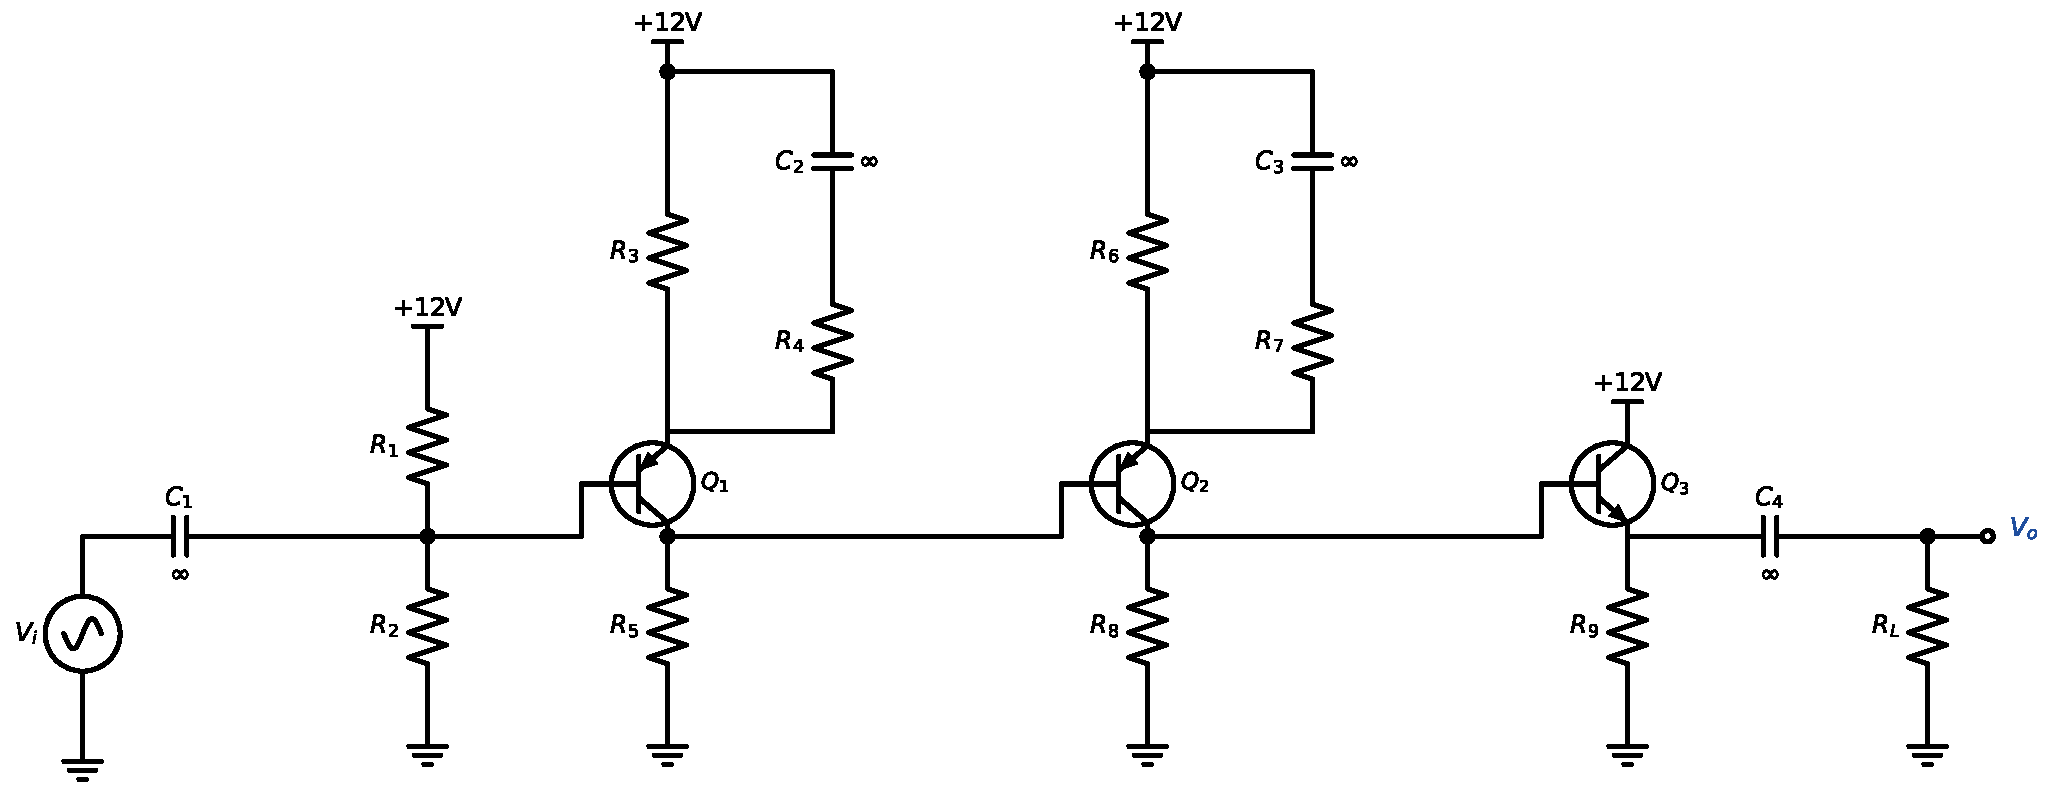
\includegraphics[width=\linewidth,height=6cm,keepaspectratio]{p18_circuit}\end{center}
\end{probbox}

\newpage
\section*{Solutions}
Every solution follows the steps of the Lecture-4 pipeline card.
\subsection*{Solution 4E.1 \hfill Easy}
\begin{center}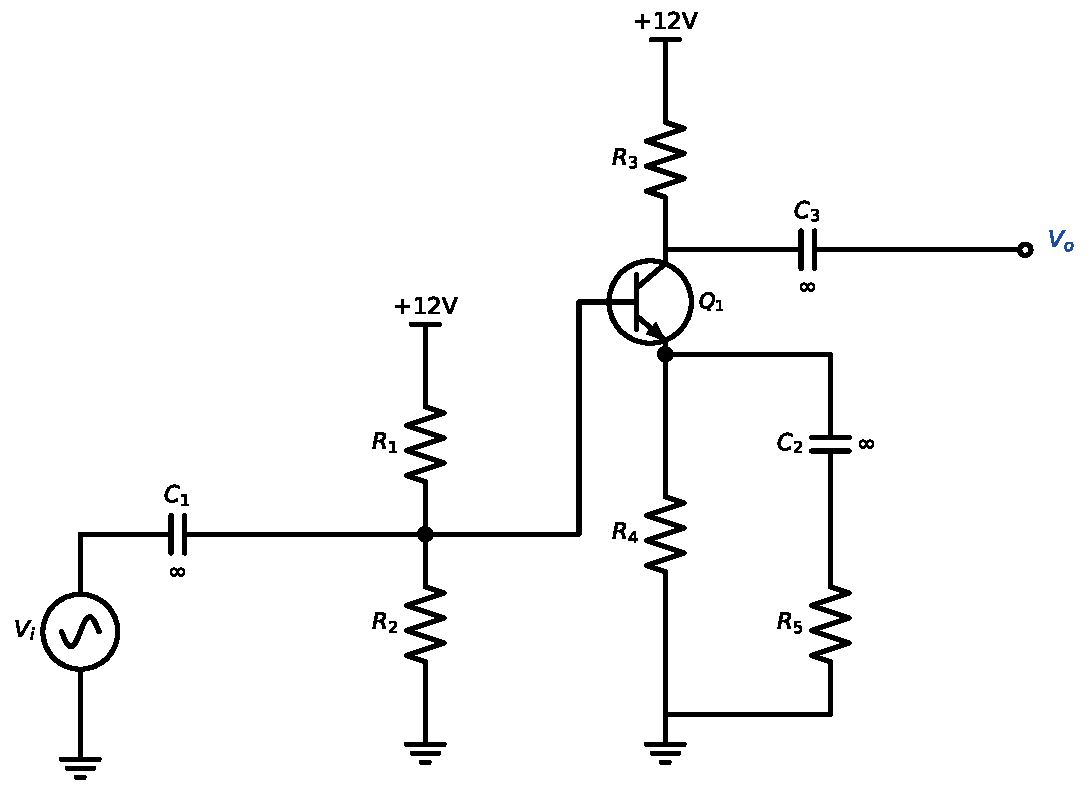
\includegraphics[width=0.9\linewidth,height=6cm,keepaspectratio]{p01_circuit}\end{center}
\solstep{1}{Plan}Name the resistors by their job: $R_{1} = R_{B1}$, $R_{2} = R_{B2}$, $R_{3} = R_{C1}$, $R_{4} = R_{E1}$, $R_{5} = R_{G1}$. Every stage is biased like the one-stage design of the slides: $V_{RE}\ge1$\,V ($V_{BE}$-insensitive), the divider and every collector current much larger than the base current it feeds ($\beta$-insensitive, factor $N$), and $V_{RC}$ as large as the swing allows. Small-signal tools: $r_e = V_T/I_C$, CE gain $|A_v| = \frac{Z_C}{r_e + R_E\|R_G}$, follower gain $\frac{Z_E}{r_e+Z_E}$, base resistance $(\beta+1)(r_e + Z_E)$ (the $\infty$ capacitors put $R_G$ in parallel with $R_E$ for AC only). Design from the output back to the input, because each stage loads the one before it.
\solstep{2}{Output stage}$V_{BE}$-insensitive: $V_{RE1} \ge 1$\,V; use $V_{RE1} = 1$\,V.

To avoid clipping at saturation the collector must be able to swing down by $\hat V_o$ without $V_{CE}$ dropping below $V_{CE,sat}$, and at cutoff $V_{RC}$ must be at least $\hat V_o$: $V_{CC} - \hat V_o - V_{RE1} - V_{CE,sat} \ge V_{RC1} \ge \hat V_o$. Take the largest value (most gain, best linearity): \[V_{RC1} = 12 - 2 - 1 - 0.2 = 8.8\,\mathrm{V} \;\ge\; \hat V_o = 2\,\mathrm{V}\ \checkmark\]

Maximum available gain ($R_G=0$, $R_C$ only): $|A_v|_{max} = \frac{R_C}{r_e} = \frac{V_{RC1}/I_C}{V_T/I_C} = \frac{V_{RC1}}{V_T} = \frac{8.8}{0.025} = 352 \ge 50$ \checkmark
\solstep{3}{Bias current and resistors}Divider: $V_{RB2} = V_{B1} = 1.7\,\mathrm{V}$, $V_{RB1} = V_{CC} - V_{B1} = 10.3\,\mathrm{V}$ ($|V_{RE1}| + 0.7$ on the emitter side). $\beta$-insensitive: the divider current is $N$ times the base current, $I_{RB} = N\frac{I_{C1}}{\beta}$, $N = 10$. Input resistance (all three in parallel, with $(\beta+1)(r_e + R_E\|R_G) \approx \beta\frac{R_{C1}}{|A_{v1}|} = \beta\frac{V_{RC1}}{I_{C1}|A_{v1}|}$):\[R_i \approx \frac{\beta/I_{C1}}{\frac{N}{V_{RB1}} + \frac{N}{V_{RB2}} + \frac{|A_{v1}|}{V_{RC1}}} \ge R_{i,spec} \;\Rightarrow\; I_{C1} \le \frac{\beta/R_{i,spec}}{\frac{10}{10.3} + \frac{10}{1.7} + \frac{50}{8.8}} = 1.6\,\mathrm{m}\mathrm{A}\]Take the E12 value just below: $I_{C1} = 1.5\,\mathrm{m}\mathrm{A}$. 

\[R_{C1} = \frac{V_{RC1}}{I_{C1}} = \frac{8.8}{1.5\,\mathrm{m}\mathrm{A}} = \mathbf{5.87\,\mathrm{k}\Omega},\quad R_{E1} = \frac{V_{RE1}}{I_{C1}} = \frac{1}{1.5\,\mathrm{m}\mathrm{A}} = \mathbf{667\,\Omega},\quad r_{e1} = \frac{V_T}{I_{C1}} = 16.7\,\Omega\]

Gain $|A_{v1}| = \frac{R_{C1}}{r_{e1} + R_{E1}\|R_{G1}} = 50$:\[R_{E1}\|R_{G1} = \frac{R_{C1}}{|A_{v1}|} - r_{e1} = 101\,\Omega \;\Rightarrow\; R_{G1} = \frac{1}{\frac{1}{101\,\Omega} - \frac{1}{667\,\Omega}} = \mathbf{119\,\Omega}\]

\[R_{B1} = \frac{V_{RB1}}{N I_{C1}/\beta} = \frac{10.3}{150\,\mu \mathrm{A}} = \mathbf{68.7\,\mathrm{k}\Omega},\qquad R_{B2} = \frac{V_{RB2}}{N I_{C1}/\beta} = \frac{1.7}{150\,\mu \mathrm{A}} = \mathbf{11.3\,\mathrm{k}\Omega}\]

Check: $R_i = R_{B1}\|R_{B2}\|(\beta+1)(r_{e1} + R_{E1}\|R_{G1}) = 68.7\,\mathrm{k}\Omega\|11.3\,\mathrm{k}\Omega\|11.9\,\mathrm{k}\Omega = 5.342\,\mathrm{k}\Omega$ $\ge 5\,\mathrm{k}\Omega$ \checkmark.
\solstep{4}{Check by analysis}Solve the finished circuit exactly ($\beta=100$, base currents included) for the DC point, then the small-signal gain with the exact $r_e$ values:\begin{center}\renewcommand{\arraystretch}{1.35}
\begin{tabular}{cccc}
\toprule
 & design $I_C$ & exact $I_C$ & exact $|V_{CE}|$ \\
\midrule
$Q_{1}$ & $1.5\,\mathrm{m}\mathrm{A}$ & $1.3\,\mathrm{m}\mathrm{A}$ & $3.513\,\mathrm{V}$ \\
\bottomrule
\end{tabular}\end{center}
The exact currents are a little off the design values: $N$ only makes each base current $N$ times smaller than the current it disturbs, so the base voltages sag slightly, and along direct-coupled stages each shift is passed on (and amplified) to the next stage. The slides handle this the same way: simulate, then adjust. The exact gain is $|A_v| = 48.43$ instead of $50$ (the hand design ignored $\alpha$ and the base currents). As the slides suggest, trim $R_{G1}$: the gain is proportional to $1/(r_{e1} + R_{E1}\|R_{G1})$, so scale that sum by $48.43/50$ (exact $r_{e1} = 19.3\,\Omega$):\[R_{E1}\|R_{G1} = (19.3\,\Omega + 101\,\Omega)\frac{48.43}{50} - 19.3\,\Omega = 96.9\,\Omega \;\Rightarrow\; R_{G1} = \mathbf{113\,\Omega}\]Re-analysis: $|A_v| = 50$ \checkmark. \begin{itemize}[leftmargin=*,itemsep=2pt]
\item Input resistance (exact): $R_i = 5.32\,\mathrm{k}\Omega$ $\ge 5\,\mathrm{k}\Omega$ \checkmark
\item Output swing: $Q_{1}$ clips (saturation or cutoff) at $\hat V_o = 3.313\,\mathrm{V}$. The smallest, $3.313\,\mathrm{V}$, is $\ge 2$\,V \checkmark
\item Distortion: each CE stage adds $HD_2 \approx \frac{\hat v_b}{4V_T}\left(\frac{r_e}{r_e + R_E\|R_G}\right)^2$ ($\hat v_b$ = its input amplitude at the specified output; for one stage this is the slides' $\frac{\hat V_o V_T |A_v|}{4V_{RC}^2}$): THD $\approx 1\,\%$ $\le 2\,\%$ \checkmark
\item $V_{BE}$-insensitive: $V_{RE1} = 1$\,V $\ge 1$\,V \checkmark
\end{itemize}

\begin{center}\renewcommand{\arraystretch}{1.35}
\begin{tabular}{ll}
\toprule
resistor & value \\
\midrule
$R_{1}$ ($R_{B1}$) & $68.7\,\mathrm{k}\Omega$ \\
$R_{2}$ ($R_{B2}$) & $11.3\,\mathrm{k}\Omega$ \\
$R_{3}$ ($R_{C1}$) & $5.87\,\mathrm{k}\Omega$ \\
$R_{4}$ ($R_{E1}$) & $667\,\Omega$ \\
$R_{5}$ ($R_{G1}$) & $113\,\Omega$ \\
\bottomrule
\end{tabular}\end{center}
\begin{center}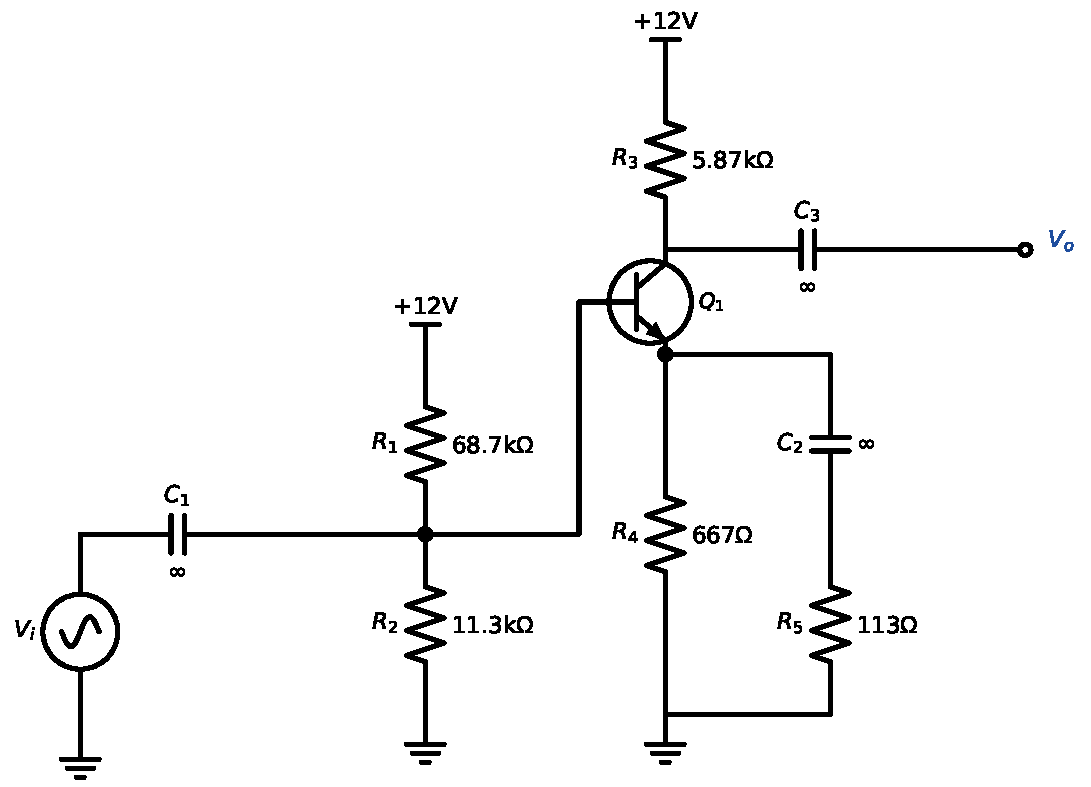
\includegraphics[width=0.9\linewidth,height=6.5cm,keepaspectratio]{p01_designed}\end{center}

\begin{ansbox}
$R_{1} = 68.7\,\mathrm{k}\Omega$,\quad $R_{2} = 11.3\,\mathrm{k}\Omega$,\quad $R_{3} = 5.87\,\mathrm{k}\Omega$,\quad $R_{4} = 667\,\Omega$,\quad $R_{5} = 113\,\Omega$
\end{ansbox}

\newpage
\subsection*{Solution 4E.2 \hfill Easy}
\begin{center}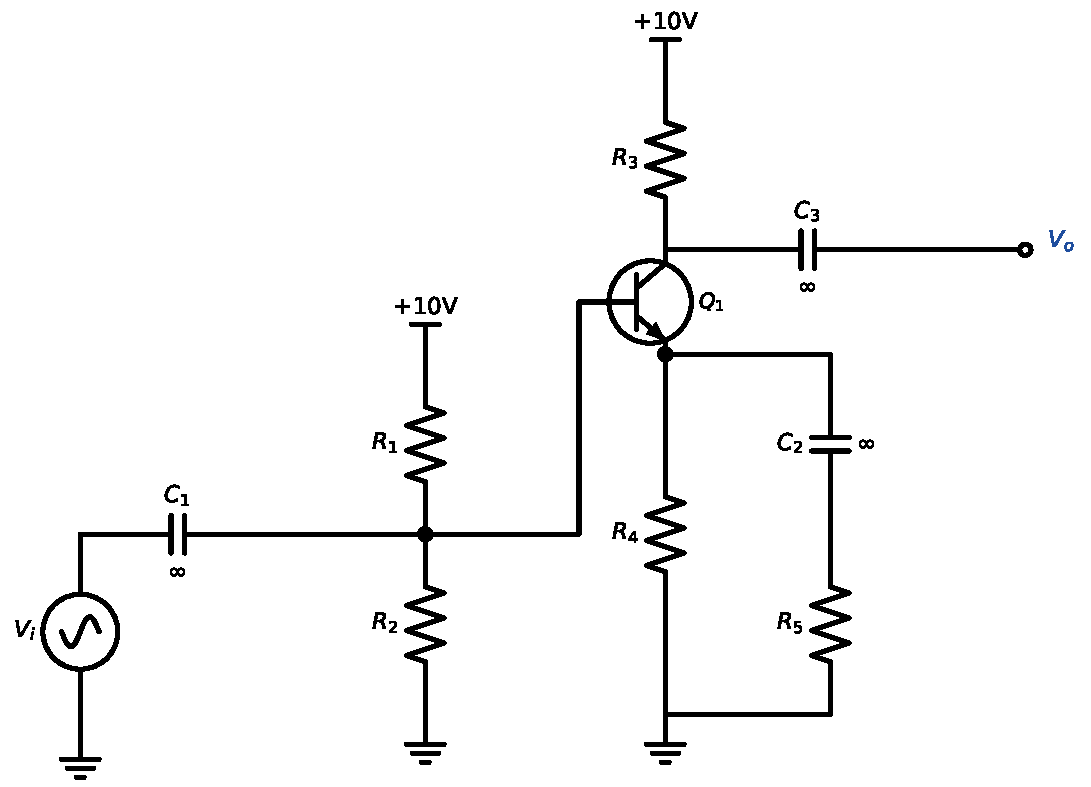
\includegraphics[width=0.9\linewidth,height=6cm,keepaspectratio]{p02_circuit}\end{center}
\solstep{1}{Plan}Name the resistors by their job: $R_{1} = R_{B1}$, $R_{2} = R_{B2}$, $R_{3} = R_{C1}$, $R_{4} = R_{E1}$, $R_{5} = R_{G1}$. Every stage is biased like the one-stage design of the slides: $V_{RE}\ge1$\,V ($V_{BE}$-insensitive), the divider and every collector current much larger than the base current it feeds ($\beta$-insensitive, factor $N$), and $V_{RC}$ as large as the swing allows. Small-signal tools: $r_e = V_T/I_C$, CE gain $|A_v| = \frac{Z_C}{r_e + R_E\|R_G}$, follower gain $\frac{Z_E}{r_e+Z_E}$, base resistance $(\beta+1)(r_e + Z_E)$ (the $\infty$ capacitors put $R_G$ in parallel with $R_E$ for AC only). Design from the output back to the input, because each stage loads the one before it.
\solstep{2}{Output stage}$V_{BE}$-insensitive: $V_{RE1} \ge 1$\,V; use $V_{RE1} = 1$\,V.

To avoid clipping at saturation the collector must be able to swing down by $\hat V_o$ without $V_{CE}$ dropping below $V_{CE,sat}$, and at cutoff $V_{RC}$ must be at least $\hat V_o$: $V_{CC} - \hat V_o - V_{RE1} - V_{CE,sat} \ge V_{RC1} \ge \hat V_o$. Take the largest value (most gain, best linearity): \[V_{RC1} = 10 - 1.5 - 1 - 0.2 = 7.3\,\mathrm{V} \;\ge\; \hat V_o = 1.5\,\mathrm{V}\ \checkmark\]

Maximum available gain ($R_G=0$, $R_C$ only): $|A_v|_{max} = \frac{R_C}{r_e} = \frac{V_{RC1}/I_C}{V_T/I_C} = \frac{V_{RC1}}{V_T} = \frac{7.3}{0.025} = 292 \ge 80$ \checkmark
\solstep{3}{Bias current and resistors}Divider: $V_{RB2} = V_{B1} = 1.7\,\mathrm{V}$, $V_{RB1} = V_{CC} - V_{B1} = 8.3\,\mathrm{V}$ ($|V_{RE1}| + 0.7$ on the emitter side). $\beta$-insensitive: the divider current is $N$ times the base current, $I_{RB} = N\frac{I_{C1}}{\beta}$, $N = 10$. Input resistance (all three in parallel, with $(\beta+1)(r_e + R_E\|R_G) \approx \beta\frac{R_{C1}}{|A_{v1}|} = \beta\frac{V_{RC1}}{I_{C1}|A_{v1}|}$):\[R_i \approx \frac{\beta/I_{C1}}{\frac{N}{V_{RB1}} + \frac{N}{V_{RB2}} + \frac{|A_{v1}|}{V_{RC1}}} \ge R_{i,spec} \;\Rightarrow\; I_{C1} \le \frac{\beta/R_{i,spec}}{\frac{10}{8.3} + \frac{10}{1.7} + \frac{80}{7.3}} = 1.85\,\mathrm{m}\mathrm{A}\]Take the E12 value just below: $I_{C1} = 1.8\,\mathrm{m}\mathrm{A}$. 

\[R_{C1} = \frac{V_{RC1}}{I_{C1}} = \frac{7.3}{1.8\,\mathrm{m}\mathrm{A}} = \mathbf{4.06\,\mathrm{k}\Omega},\quad R_{E1} = \frac{V_{RE1}}{I_{C1}} = \frac{1}{1.8\,\mathrm{m}\mathrm{A}} = \mathbf{556\,\Omega},\quad r_{e1} = \frac{V_T}{I_{C1}} = 13.9\,\Omega\]

Gain $|A_{v1}| = \frac{R_{C1}}{r_{e1} + R_{E1}\|R_{G1}} = 80$:\[R_{E1}\|R_{G1} = \frac{R_{C1}}{|A_{v1}|} - r_{e1} = 36.8\,\Omega \;\Rightarrow\; R_{G1} = \frac{1}{\frac{1}{36.8\,\Omega} - \frac{1}{556\,\Omega}} = \mathbf{39.4\,\Omega}\]

\[R_{B1} = \frac{V_{RB1}}{N I_{C1}/\beta} = \frac{8.3}{180\,\mu \mathrm{A}} = \mathbf{46.1\,\mathrm{k}\Omega},\qquad R_{B2} = \frac{V_{RB2}}{N I_{C1}/\beta} = \frac{1.7}{180\,\mu \mathrm{A}} = \mathbf{9.44\,\mathrm{k}\Omega}\]

Check: $R_i = R_{B1}\|R_{B2}\|(\beta+1)(r_{e1} + R_{E1}\|R_{G1}) = 46.1\,\mathrm{k}\Omega\|9.44\,\mathrm{k}\Omega\|5.12\,\mathrm{k}\Omega = 3.097\,\mathrm{k}\Omega$ $\ge 3\,\mathrm{k}\Omega$ \checkmark.
\solstep{4}{Check by analysis}Solve the finished circuit exactly ($\beta=100$, base currents included) for the DC point, then the small-signal gain with the exact $r_e$ values:\begin{center}\renewcommand{\arraystretch}{1.35}
\begin{tabular}{cccc}
\toprule
 & design $I_C$ & exact $I_C$ & exact $|V_{CE}|$ \\
\midrule
$Q_{1}$ & $1.8\,\mathrm{m}\mathrm{A}$ & $1.56\,\mathrm{m}\mathrm{A}$ & $2.781\,\mathrm{V}$ \\
\bottomrule
\end{tabular}\end{center}
The exact currents are a little off the design values: $N$ only makes each base current $N$ times smaller than the current it disturbs, so the base voltages sag slightly, and along direct-coupled stages each shift is passed on (and amplified) to the next stage. The slides handle this the same way: simulate, then adjust. The exact gain is $|A_v| = 76.06$ instead of $80$ (the hand design ignored $\alpha$ and the base currents). As the slides suggest, trim $R_{G1}$: the gain is proportional to $1/(r_{e1} + R_{E1}\|R_{G1})$, so scale that sum by $76.06/80$ (exact $r_{e1} = 16\,\Omega$):\[R_{E1}\|R_{G1} = (16\,\Omega + 36.8\,\Omega)\frac{76.06}{80} - 16\,\Omega = 34.2\,\Omega \;\Rightarrow\; R_{G1} = \mathbf{36.4\,\Omega}\]Re-analysis: $|A_v| = 80$ \checkmark. \begin{itemize}[leftmargin=*,itemsep=2pt]
\item Input resistance (exact): $R_i = 3.08\,\mathrm{k}\Omega$ $\ge 3\,\mathrm{k}\Omega$ \checkmark
\item Output swing: $Q_{1}$ clips (saturation or cutoff) at $\hat V_o = 2.581\,\mathrm{V}$. The smallest, $2.581\,\mathrm{V}$, is $\ge 1.5$\,V \checkmark
\item Distortion: each CE stage adds $HD_2 \approx \frac{\hat v_b}{4V_T}\left(\frac{r_e}{r_e + R_E\|R_G}\right)^2$ ($\hat v_b$ = its input amplitude at the specified output; for one stage this is the slides' $\frac{\hat V_o V_T |A_v|}{4V_{RC}^2}$): THD $\approx 1.7\,\%$ $\le 3\,\%$ \checkmark
\item $V_{BE}$-insensitive: $V_{RE1} = 1$\,V $\ge 1$\,V \checkmark
\end{itemize}

\begin{center}\renewcommand{\arraystretch}{1.35}
\begin{tabular}{ll}
\toprule
resistor & value \\
\midrule
$R_{1}$ ($R_{B1}$) & $46.1\,\mathrm{k}\Omega$ \\
$R_{2}$ ($R_{B2}$) & $9.44\,\mathrm{k}\Omega$ \\
$R_{3}$ ($R_{C1}$) & $4.06\,\mathrm{k}\Omega$ \\
$R_{4}$ ($R_{E1}$) & $556\,\Omega$ \\
$R_{5}$ ($R_{G1}$) & $36.4\,\Omega$ \\
\bottomrule
\end{tabular}\end{center}
\begin{center}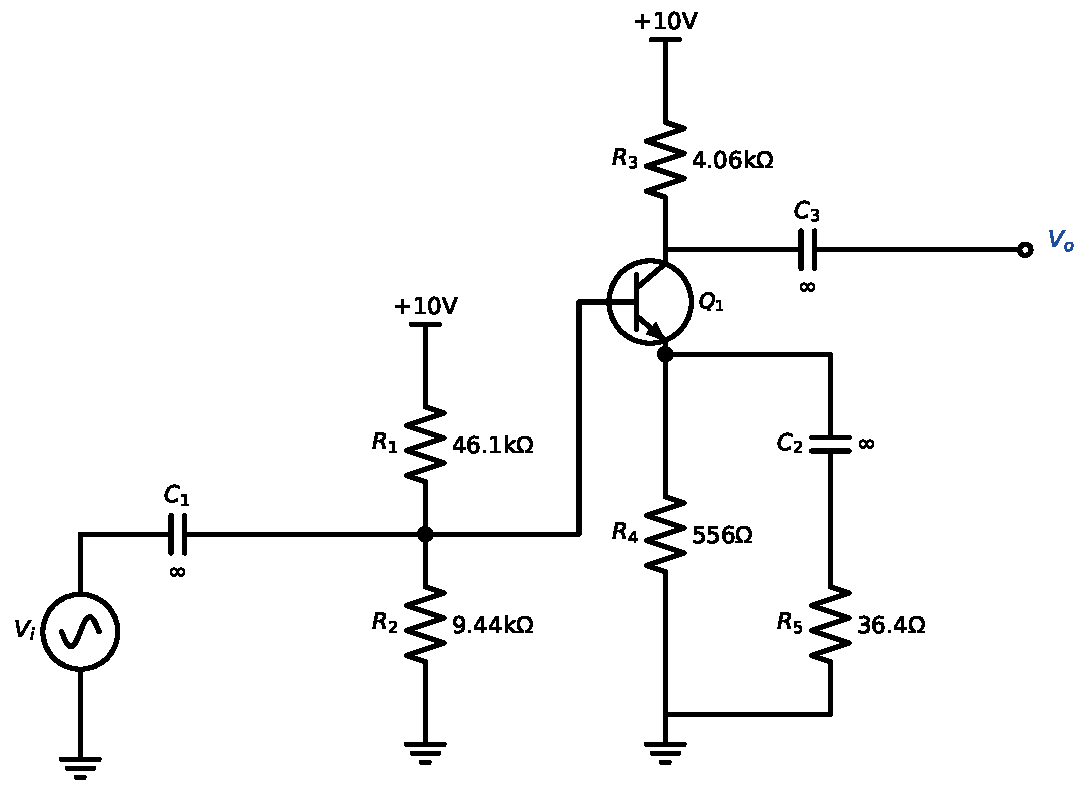
\includegraphics[width=0.9\linewidth,height=6.5cm,keepaspectratio]{p02_designed}\end{center}

\begin{ansbox}
$R_{1} = 46.1\,\mathrm{k}\Omega$,\quad $R_{2} = 9.44\,\mathrm{k}\Omega$,\quad $R_{3} = 4.06\,\mathrm{k}\Omega$,\quad $R_{4} = 556\,\Omega$,\quad $R_{5} = 36.4\,\Omega$
\end{ansbox}

\newpage
\subsection*{Solution 4E.3 \hfill Easy}
\begin{center}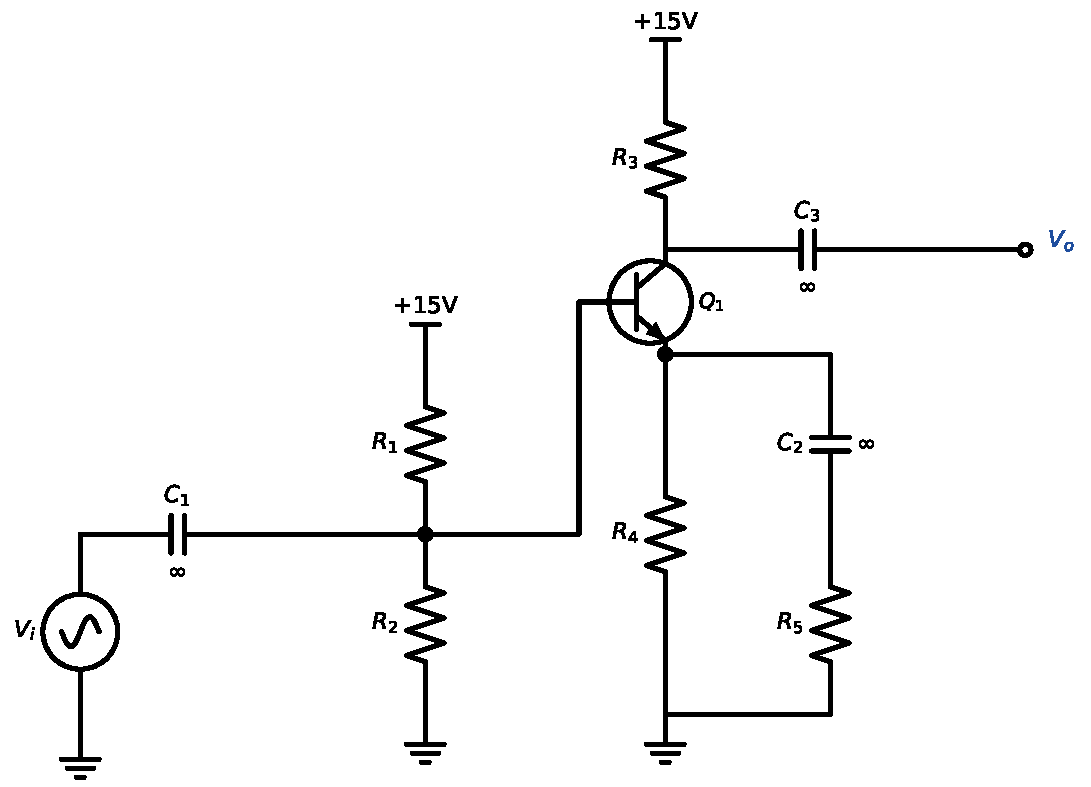
\includegraphics[width=0.9\linewidth,height=6cm,keepaspectratio]{p03_circuit}\end{center}
\solstep{1}{Plan}Name the resistors by their job: $R_{1} = R_{B1}$, $R_{2} = R_{B2}$, $R_{3} = R_{C1}$, $R_{4} = R_{E1}$, $R_{5} = R_{G1}$. Every stage is biased like the one-stage design of the slides: $V_{RE}\ge1$\,V ($V_{BE}$-insensitive), the divider and every collector current much larger than the base current it feeds ($\beta$-insensitive, factor $N$), and $V_{RC}$ as large as the swing allows. Small-signal tools: $r_e = V_T/I_C$, CE gain $|A_v| = \frac{Z_C}{r_e + R_E\|R_G}$, follower gain $\frac{Z_E}{r_e+Z_E}$, base resistance $(\beta+1)(r_e + Z_E)$ (the $\infty$ capacitors put $R_G$ in parallel with $R_E$ for AC only). Design from the output back to the input, because each stage loads the one before it.
\solstep{2}{Output stage}$V_{BE}$-insensitive: $V_{RE1} \ge 1$\,V; use $V_{RE1} = 1$\,V.

To avoid clipping at saturation the collector must be able to swing down by $\hat V_o$ without $V_{CE}$ dropping below $V_{CE,sat}$, and at cutoff $V_{RC}$ must be at least $\hat V_o$: $V_{CC} - \hat V_o - V_{RE1} - V_{CE,sat} \ge V_{RC1} \ge \hat V_o$. Take the largest value (most gain, best linearity): \[V_{RC1} = 15 - 3 - 1 - 0.2 = 10.8\,\mathrm{V} \;\ge\; \hat V_o = 3\,\mathrm{V}\ \checkmark\]

Maximum available gain ($R_G=0$, $R_C$ only): $|A_v|_{max} = \frac{R_C}{r_e} = \frac{V_{RC1}/I_C}{V_T/I_C} = \frac{V_{RC1}}{V_T} = \frac{10.8}{0.025} = 432 \ge 30$ \checkmark
\solstep{3}{Bias current and resistors}Divider: $V_{RB2} = V_{B1} = 1.7\,\mathrm{V}$, $V_{RB1} = V_{CC} - V_{B1} = 13.3\,\mathrm{V}$ ($|V_{RE1}| + 0.7$ on the emitter side). $\beta$-insensitive: the divider current is $N$ times the base current, $I_{RB} = N\frac{I_{C1}}{\beta}$, $N = 10$. Input resistance (all three in parallel, with $(\beta+1)(r_e + R_E\|R_G) \approx \beta\frac{R_{C1}}{|A_{v1}|} = \beta\frac{V_{RC1}}{I_{C1}|A_{v1}|}$):\[R_i \approx \frac{\beta/I_{C1}}{\frac{N}{V_{RB1}} + \frac{N}{V_{RB2}} + \frac{|A_{v1}|}{V_{RC1}}} \ge R_{i,spec} \;\Rightarrow\; I_{C1} \le \frac{\beta/R_{i,spec}}{\frac{10}{13.3} + \frac{10}{1.7} + \frac{30}{10.8}} = 1.06\,\mathrm{m}\mathrm{A}\]Take the E12 value just below: $I_{C1} = 1\,\mathrm{m}\mathrm{A}$. 

\[R_{C1} = \frac{V_{RC1}}{I_{C1}} = \frac{10.8}{1\,\mathrm{m}\mathrm{A}} = \mathbf{10.8\,\mathrm{k}\Omega},\quad R_{E1} = \frac{V_{RE1}}{I_{C1}} = \frac{1}{1\,\mathrm{m}\mathrm{A}} = \mathbf{1\,\mathrm{k}\Omega},\quad r_{e1} = \frac{V_T}{I_{C1}} = 25\,\Omega\]

Gain $|A_{v1}| = \frac{R_{C1}}{r_{e1} + R_{E1}\|R_{G1}} = 30$:\[R_{E1}\|R_{G1} = \frac{R_{C1}}{|A_{v1}|} - r_{e1} = 335\,\Omega \;\Rightarrow\; R_{G1} = \frac{1}{\frac{1}{335\,\Omega} - \frac{1}{1\,\mathrm{k}\Omega}} = \mathbf{504\,\Omega}\]

\[R_{B1} = \frac{V_{RB1}}{N I_{C1}/\beta} = \frac{13.3}{100\,\mu \mathrm{A}} = \mathbf{133\,\mathrm{k}\Omega},\qquad R_{B2} = \frac{V_{RB2}}{N I_{C1}/\beta} = \frac{1.7}{100\,\mu \mathrm{A}} = \mathbf{17\,\mathrm{k}\Omega}\]

Check: $R_i = R_{B1}\|R_{B2}\|(\beta+1)(r_{e1} + R_{E1}\|R_{G1}) = 133\,\mathrm{k}\Omega\|17\,\mathrm{k}\Omega\|36.4\,\mathrm{k}\Omega = 10.66\,\mathrm{k}\Omega$ $\ge 10\,\mathrm{k}\Omega$ \checkmark.
\solstep{4}{Check by analysis}Solve the finished circuit exactly ($\beta=100$, base currents included) for the DC point, then the small-signal gain with the exact $r_e$ values:\begin{center}\renewcommand{\arraystretch}{1.35}
\begin{tabular}{cccc}
\toprule
 & design $I_C$ & exact $I_C$ & exact $|V_{CE}|$ \\
\midrule
$Q_{1}$ & $1\,\mathrm{m}\mathrm{A}$ & $862\,\mu \mathrm{A}$ & $4.825\,\mathrm{V}$ \\
\bottomrule
\end{tabular}\end{center}
The exact currents are a little off the design values: $N$ only makes each base current $N$ times smaller than the current it disturbs, so the base voltages sag slightly, and along direct-coupled stages each shift is passed on (and amplified) to the next stage. The slides handle this the same way: simulate, then adjust. The exact gain is $|A_v| = 29.38$ instead of $30$ (the hand design ignored $\alpha$ and the base currents). As the slides suggest, trim $R_{G1}$: the gain is proportional to $1/(r_{e1} + R_{E1}\|R_{G1})$, so scale that sum by $29.38/30$ (exact $r_{e1} = 29\,\Omega$):\[R_{E1}\|R_{G1} = (29\,\Omega + 335\,\Omega)\frac{29.38}{30} - 29\,\Omega = 327\,\Omega \;\Rightarrow\; R_{G1} = \mathbf{487\,\Omega}\]Re-analysis: $|A_v| = 30$ \checkmark. \begin{itemize}[leftmargin=*,itemsep=2pt]
\item Input resistance (exact): $R_i = 10.6\,\mathrm{k}\Omega$ $\ge 10\,\mathrm{k}\Omega$ \checkmark
\item Output swing: $Q_{1}$ clips (saturation or cutoff) at $\hat V_o = 4.625\,\mathrm{V}$. The smallest, $4.625\,\mathrm{V}$, is $\ge 3$\,V \checkmark
\item Distortion: each CE stage adds $HD_2 \approx \frac{\hat v_b}{4V_T}\left(\frac{r_e}{r_e + R_E\|R_G}\right)^2$ ($\hat v_b$ = its input amplitude at the specified output; for one stage this is the slides' $\frac{\hat V_o V_T |A_v|}{4V_{RC}^2}$): THD $\approx 0.64\,\%$ $\le 2\,\%$ \checkmark
\item $V_{BE}$-insensitive: $V_{RE1} = 1$\,V $\ge 1$\,V \checkmark
\end{itemize}

\begin{center}\renewcommand{\arraystretch}{1.35}
\begin{tabular}{ll}
\toprule
resistor & value \\
\midrule
$R_{1}$ ($R_{B1}$) & $133\,\mathrm{k}\Omega$ \\
$R_{2}$ ($R_{B2}$) & $17\,\mathrm{k}\Omega$ \\
$R_{3}$ ($R_{C1}$) & $10.8\,\mathrm{k}\Omega$ \\
$R_{4}$ ($R_{E1}$) & $1\,\mathrm{k}\Omega$ \\
$R_{5}$ ($R_{G1}$) & $487\,\Omega$ \\
\bottomrule
\end{tabular}\end{center}
\begin{center}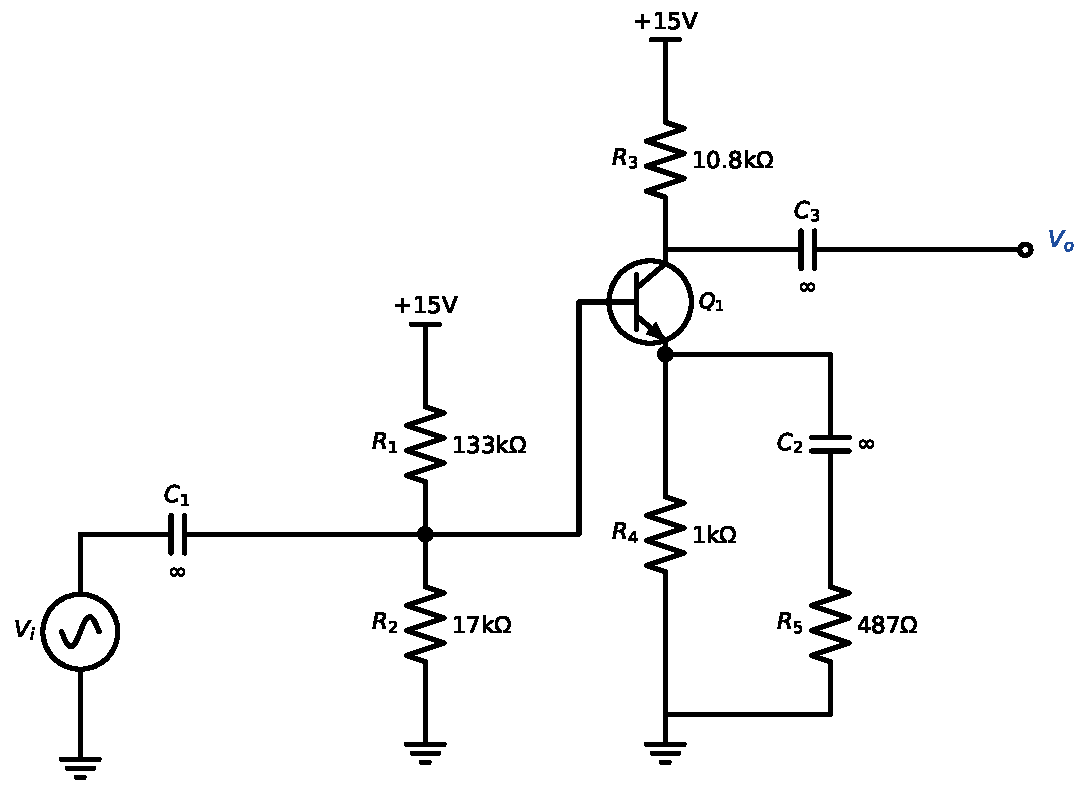
\includegraphics[width=0.9\linewidth,height=6.5cm,keepaspectratio]{p03_designed}\end{center}

\begin{ansbox}
$R_{1} = 133\,\mathrm{k}\Omega$,\quad $R_{2} = 17\,\mathrm{k}\Omega$,\quad $R_{3} = 10.8\,\mathrm{k}\Omega$,\quad $R_{4} = 1\,\mathrm{k}\Omega$,\quad $R_{5} = 487\,\Omega$
\end{ansbox}

\newpage
\subsection*{Solution 4E.4 \hfill Easy}
\begin{center}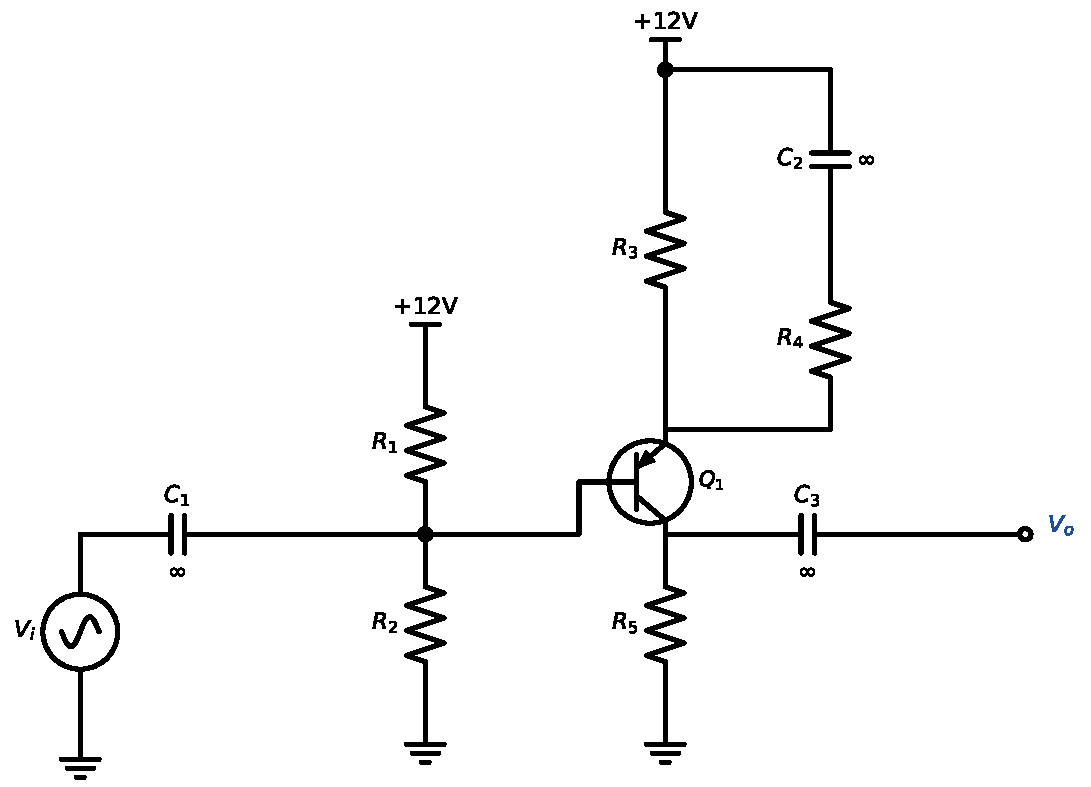
\includegraphics[width=0.9\linewidth,height=6cm,keepaspectratio]{p04_circuit}\end{center}
\solstep{1}{Plan}Name the resistors by their job: $R_{1} = R_{B1}$, $R_{2} = R_{B2}$, $R_{3} = R_{E1}$, $R_{4} = R_{G1}$, $R_{5} = R_{C1}$. Every stage is biased like the one-stage design of the slides: $V_{RE}\ge1$\,V ($V_{BE}$-insensitive), the divider and every collector current much larger than the base current it feeds ($\beta$-insensitive, factor $N$), and $V_{RC}$ as large as the swing allows. Small-signal tools: $r_e = V_T/I_C$, CE gain $|A_v| = \frac{Z_C}{r_e + R_E\|R_G}$, follower gain $\frac{Z_E}{r_e+Z_E}$, base resistance $(\beta+1)(r_e + Z_E)$ (the $\infty$ capacitors put $R_G$ in parallel with $R_E$ for AC only). Design from the output back to the input, because each stage loads the one before it.
\solstep{2}{Output stage}$V_{BE}$-insensitive: $V_{RE1} \ge 1$\,V; use $V_{RE1} = 1$\,V.

To avoid clipping at saturation the collector must be able to swing down by $\hat V_o$ without $V_{CE}$ dropping below $V_{CE,sat}$, and at cutoff $V_{RC}$ must be at least $\hat V_o$: $V_{CC} - \hat V_o - V_{RE1} - V_{CE,sat} \ge V_{RC1} \ge \hat V_o$. Take the largest value (most gain, best linearity): \[V_{RC1} = 12 - 2 - 1 - 0.2 = 8.8\,\mathrm{V} \;\ge\; \hat V_o = 2\,\mathrm{V}\ \checkmark\]

Maximum available gain ($R_G=0$, $R_C$ only): $|A_v|_{max} = \frac{R_C}{r_e} = \frac{V_{RC1}/I_C}{V_T/I_C} = \frac{V_{RC1}}{V_T} = \frac{8.8}{0.025} = 352 \ge 40$ \checkmark
\solstep{3}{Bias current and resistors}Divider: $V_{RB2} = V_{B1} = 10.3\,\mathrm{V}$, $V_{RB1} = V_{CC} - V_{B1} = 1.7\,\mathrm{V}$ ($|V_{RE1}| + 0.7$ on the emitter side). $\beta$-insensitive: the divider current is $N$ times the base current, $I_{RB} = N\frac{I_{C1}}{\beta}$, $N = 10$. Input resistance (all three in parallel, with $(\beta+1)(r_e + R_E\|R_G) \approx \beta\frac{R_{C1}}{|A_{v1}|} = \beta\frac{V_{RC1}}{I_{C1}|A_{v1}|}$):\[R_i \approx \frac{\beta/I_{C1}}{\frac{N}{V_{RB1}} + \frac{N}{V_{RB2}} + \frac{|A_{v1}|}{V_{RC1}}} \ge R_{i,spec} \;\Rightarrow\; I_{C1} \le \frac{\beta/R_{i,spec}}{\frac{10}{1.7} + \frac{10}{10.3} + \frac{40}{8.8}} = 2.19\,\mathrm{m}\mathrm{A}\]Take the E12 value just below: $I_{C1} = 1.8\,\mathrm{m}\mathrm{A}$. 

\[R_{C1} = \frac{V_{RC1}}{I_{C1}} = \frac{8.8}{1.8\,\mathrm{m}\mathrm{A}} = \mathbf{4.89\,\mathrm{k}\Omega},\quad R_{E1} = \frac{V_{RE1}}{I_{C1}} = \frac{1}{1.8\,\mathrm{m}\mathrm{A}} = \mathbf{556\,\Omega},\quad r_{e1} = \frac{V_T}{I_{C1}} = 13.9\,\Omega\]

Gain $|A_{v1}| = \frac{R_{C1}}{r_{e1} + R_{E1}\|R_{G1}} = 40$:\[R_{E1}\|R_{G1} = \frac{R_{C1}}{|A_{v1}|} - r_{e1} = 108\,\Omega \;\Rightarrow\; R_{G1} = \frac{1}{\frac{1}{108\,\Omega} - \frac{1}{556\,\Omega}} = \mathbf{135\,\Omega}\]

\[R_{B1} = \frac{V_{RB1}}{N I_{C1}/\beta} = \frac{1.7}{180\,\mu \mathrm{A}} = \mathbf{9.44\,\mathrm{k}\Omega},\qquad R_{B2} = \frac{V_{RB2}}{N I_{C1}/\beta} = \frac{10.3}{180\,\mu \mathrm{A}} = \mathbf{57.2\,\mathrm{k}\Omega}\]

Check: $R_i = R_{B1}\|R_{B2}\|(\beta+1)(r_{e1} + R_{E1}\|R_{G1}) = 9.44\,\mathrm{k}\Omega\|57.2\,\mathrm{k}\Omega\|12.3\,\mathrm{k}\Omega = 4.893\,\mathrm{k}\Omega$ $\ge 4\,\mathrm{k}\Omega$ \checkmark.
\solstep{4}{Check by analysis}Solve the finished circuit exactly ($\beta=100$, base currents included) for the DC point, then the small-signal gain with the exact $r_e$ values:\begin{center}\renewcommand{\arraystretch}{1.35}
\begin{tabular}{cccc}
\toprule
 & design $I_C$ & exact $I_C$ & exact $|V_{CE}|$ \\
\midrule
$Q_{1}$ & $1.8\,\mathrm{m}\mathrm{A}$ & $1.56\,\mathrm{m}\mathrm{A}$ & $3.513\,\mathrm{V}$ \\
\bottomrule
\end{tabular}\end{center}
The exact currents are a little off the design values: $N$ only makes each base current $N$ times smaller than the current it disturbs, so the base voltages sag slightly, and along direct-coupled stages each shift is passed on (and amplified) to the next stage. The slides handle this the same way: simulate, then adjust. The exact gain is $|A_v| = 38.91$ instead of $40$ (the hand design ignored $\alpha$ and the base currents). As the slides suggest, trim $R_{G1}$: the gain is proportional to $1/(r_{e1} + R_{E1}\|R_{G1})$, so scale that sum by $38.91/40$ (exact $r_{e1} = 16.1\,\Omega$):\[R_{E1}\|R_{G1} = (16.1\,\Omega + 108\,\Omega)\frac{38.91}{40} - 16.1\,\Omega = 105\,\Omega \;\Rightarrow\; R_{G1} = \mathbf{129\,\Omega}\]Re-analysis: $|A_v| = 40$ \checkmark. \begin{itemize}[leftmargin=*,itemsep=2pt]
\item Input resistance (exact): $R_i = 4.87\,\mathrm{k}\Omega$ $\ge 4\,\mathrm{k}\Omega$ \checkmark
\item Output swing: $Q_{1}$ clips (saturation or cutoff) at $\hat V_o = 3.313\,\mathrm{V}$. The smallest, $3.313\,\mathrm{V}$, is $\ge 2$\,V \checkmark
\item Distortion: each CE stage adds $HD_2 \approx \frac{\hat v_b}{4V_T}\left(\frac{r_e}{r_e + R_E\|R_G}\right)^2$ ($\hat v_b$ = its input amplitude at the specified output; for one stage this is the slides' $\frac{\hat V_o V_T |A_v|}{4V_{RC}^2}$): THD $\approx 0.83\,\%$ $\le 2\,\%$ \checkmark
\item $V_{BE}$-insensitive: $V_{RE1} = 1$\,V $\ge 1$\,V \checkmark
\end{itemize}

\begin{center}\renewcommand{\arraystretch}{1.35}
\begin{tabular}{ll}
\toprule
resistor & value \\
\midrule
$R_{1}$ ($R_{B1}$) & $9.44\,\mathrm{k}\Omega$ \\
$R_{2}$ ($R_{B2}$) & $57.2\,\mathrm{k}\Omega$ \\
$R_{3}$ ($R_{E1}$) & $556\,\Omega$ \\
$R_{4}$ ($R_{G1}$) & $129\,\Omega$ \\
$R_{5}$ ($R_{C1}$) & $4.89\,\mathrm{k}\Omega$ \\
\bottomrule
\end{tabular}\end{center}
\begin{center}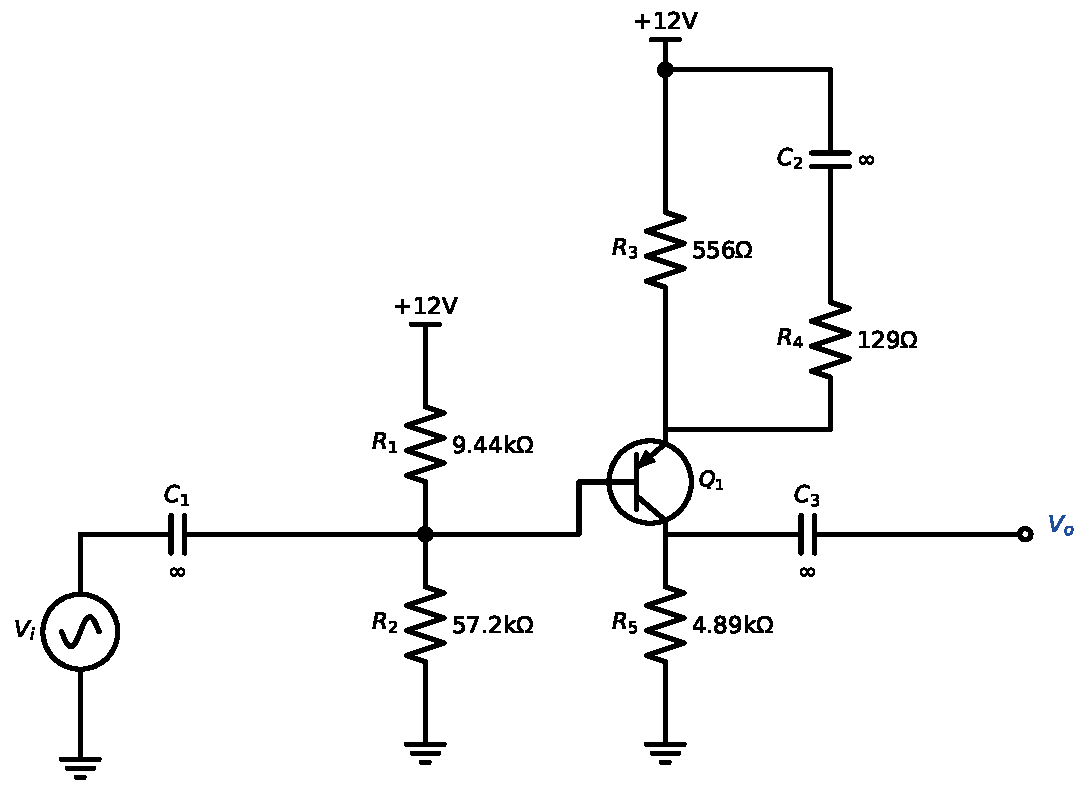
\includegraphics[width=0.9\linewidth,height=6.5cm,keepaspectratio]{p04_designed}\end{center}

\begin{ansbox}
$R_{1} = 9.44\,\mathrm{k}\Omega$,\quad $R_{2} = 57.2\,\mathrm{k}\Omega$,\quad $R_{3} = 556\,\Omega$,\quad $R_{4} = 129\,\Omega$,\quad $R_{5} = 4.89\,\mathrm{k}\Omega$
\end{ansbox}

\newpage
\subsection*{Solution 4E.5 \hfill Easy}
\begin{center}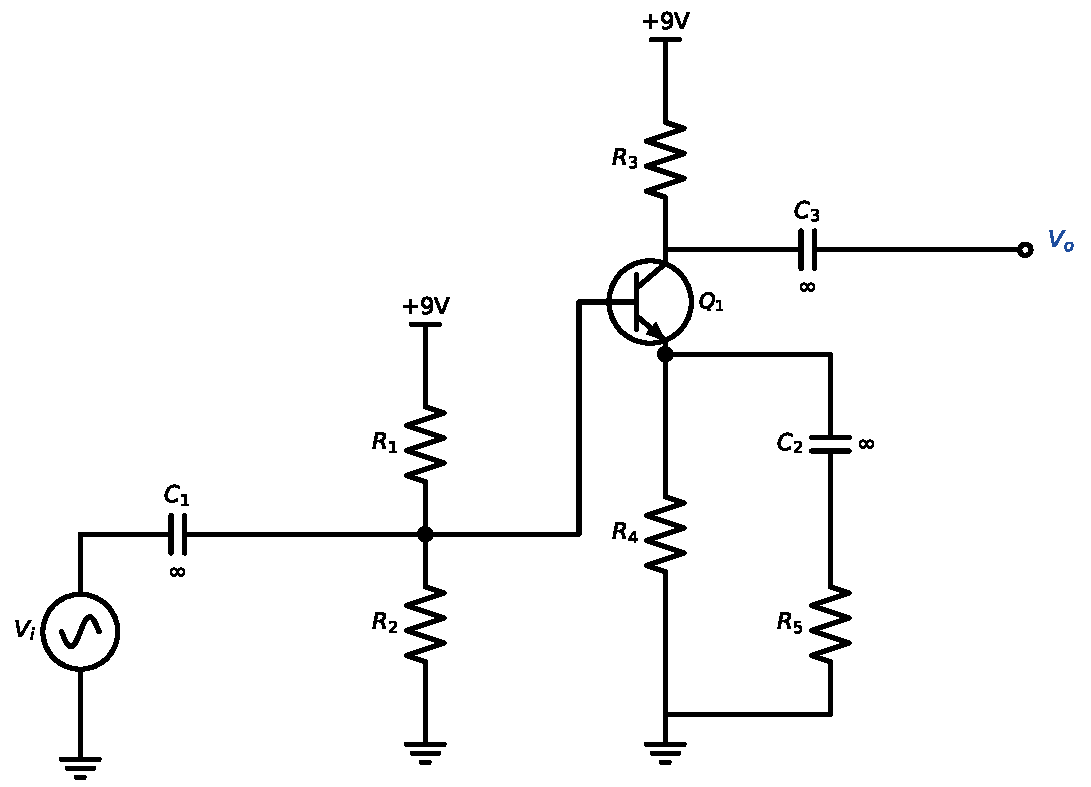
\includegraphics[width=0.9\linewidth,height=6cm,keepaspectratio]{p05_circuit}\end{center}
\solstep{1}{Plan}Name the resistors by their job: $R_{1} = R_{B1}$, $R_{2} = R_{B2}$, $R_{3} = R_{C1}$, $R_{4} = R_{E1}$, $R_{5} = R_{G1}$. Every stage is biased like the one-stage design of the slides: $V_{RE}\ge1$\,V ($V_{BE}$-insensitive), the divider and every collector current much larger than the base current it feeds ($\beta$-insensitive, factor $N$), and $V_{RC}$ as large as the swing allows. Small-signal tools: $r_e = V_T/I_C$, CE gain $|A_v| = \frac{Z_C}{r_e + R_E\|R_G}$, follower gain $\frac{Z_E}{r_e+Z_E}$, base resistance $(\beta+1)(r_e + Z_E)$ (the $\infty$ capacitors put $R_G$ in parallel with $R_E$ for AC only). Design from the output back to the input, because each stage loads the one before it.
\solstep{2}{Output stage}$V_{BE}$-insensitive: $V_{RE1} \ge 1$\,V; use $V_{RE1} = 1$\,V.

To avoid clipping at saturation the collector must be able to swing down by $\hat V_o$ without $V_{CE}$ dropping below $V_{CE,sat}$, and at cutoff $V_{RC}$ must be at least $\hat V_o$: $V_{CC} - \hat V_o - V_{RE1} - V_{CE,sat} \ge V_{RC1} \ge \hat V_o$. Take the largest value (most gain, best linearity): \[V_{RC1} = 9 - 1 - 1 - 0.2 = 6.8\,\mathrm{V} \;\ge\; \hat V_o = 1\,\mathrm{V}\ \checkmark\]

Maximum available gain ($R_G=0$, $R_C$ only): $|A_v|_{max} = \frac{R_C}{r_e} = \frac{V_{RC1}/I_C}{V_T/I_C} = \frac{V_{RC1}}{V_T} = \frac{6.8}{0.025} = 272 \ge 100$ \checkmark
\solstep{3}{Bias current and resistors}Divider: $V_{RB2} = V_{B1} = 1.7\,\mathrm{V}$, $V_{RB1} = V_{CC} - V_{B1} = 7.3\,\mathrm{V}$ ($|V_{RE1}| + 0.7$ on the emitter side). $\beta$-insensitive: the divider current is $N$ times the base current, $I_{RB} = N\frac{I_{C1}}{\beta}$, $N = 10$. Input resistance (all three in parallel, with $(\beta+1)(r_e + R_E\|R_G) \approx \beta\frac{R_{C1}}{|A_{v1}|} = \beta\frac{V_{RC1}}{I_{C1}|A_{v1}|}$):\[R_i \approx \frac{\beta/I_{C1}}{\frac{N}{V_{RB1}} + \frac{N}{V_{RB2}} + \frac{|A_{v1}|}{V_{RC1}}} \ge R_{i,spec} \;\Rightarrow\; I_{C1} \le \frac{\beta/R_{i,spec}}{\frac{10}{7.3} + \frac{10}{1.7} + \frac{100}{6.8}} = 2.28\,\mathrm{m}\mathrm{A}\]Take the E12 value just below: $I_{C1} = 2.2\,\mathrm{m}\mathrm{A}$. 

\[R_{C1} = \frac{V_{RC1}}{I_{C1}} = \frac{6.8}{2.2\,\mathrm{m}\mathrm{A}} = \mathbf{3.09\,\mathrm{k}\Omega},\quad R_{E1} = \frac{V_{RE1}}{I_{C1}} = \frac{1}{2.2\,\mathrm{m}\mathrm{A}} = \mathbf{455\,\Omega},\quad r_{e1} = \frac{V_T}{I_{C1}} = 11.4\,\Omega\]

Gain $|A_{v1}| = \frac{R_{C1}}{r_{e1} + R_{E1}\|R_{G1}} = 100$:\[R_{E1}\|R_{G1} = \frac{R_{C1}}{|A_{v1}|} - r_{e1} = 19.5\,\Omega \;\Rightarrow\; R_{G1} = \frac{1}{\frac{1}{19.5\,\Omega} - \frac{1}{455\,\Omega}} = \mathbf{20.4\,\Omega}\]

\[R_{B1} = \frac{V_{RB1}}{N I_{C1}/\beta} = \frac{7.3}{220\,\mu \mathrm{A}} = \mathbf{33.2\,\mathrm{k}\Omega},\qquad R_{B2} = \frac{V_{RB2}}{N I_{C1}/\beta} = \frac{1.7}{220\,\mu \mathrm{A}} = \mathbf{7.73\,\mathrm{k}\Omega}\]

Check: $R_i = R_{B1}\|R_{B2}\|(\beta+1)(r_{e1} + R_{E1}\|R_{G1}) = 33.2\,\mathrm{k}\Omega\|7.73\,\mathrm{k}\Omega\|3.12\,\mathrm{k}\Omega = 2.084\,\mathrm{k}\Omega$ $\ge 2\,\mathrm{k}\Omega$ \checkmark.
\solstep{4}{Check by analysis}Solve the finished circuit exactly ($\beta=100$, base currents included) for the DC point, then the small-signal gain with the exact $r_e$ values:\begin{center}\renewcommand{\arraystretch}{1.35}
\begin{tabular}{cccc}
\toprule
 & design $I_C$ & exact $I_C$ & exact $|V_{CE}|$ \\
\midrule
$Q_{1}$ & $2.2\,\mathrm{m}\mathrm{A}$ & $1.92\,\mathrm{m}\mathrm{A}$ & $2.196\,\mathrm{V}$ \\
\bottomrule
\end{tabular}\end{center}
The exact currents are a little off the design values: $N$ only makes each base current $N$ times smaller than the current it disturbs, so the base voltages sag slightly, and along direct-coupled stages each shift is passed on (and amplified) to the next stage. The slides handle this the same way: simulate, then adjust. The exact gain is $|A_v| = 93.9$ instead of $100$ (the hand design ignored $\alpha$ and the base currents). As the slides suggest, trim $R_{G1}$: the gain is proportional to $1/(r_{e1} + R_{E1}\|R_{G1})$, so scale that sum by $93.9/100$ (exact $r_{e1} = 13\,\Omega$):\[R_{E1}\|R_{G1} = (13\,\Omega + 19.5\,\Omega)\frac{93.9}{100} - 13\,\Omega = 17.6\,\Omega \;\Rightarrow\; R_{G1} = \mathbf{18.3\,\Omega}\]Re-analysis: $|A_v| = 100$ \checkmark. \begin{itemize}[leftmargin=*,itemsep=2pt]
\item Input resistance (exact): $R_i = 2.07\,\mathrm{k}\Omega$ $\ge 2\,\mathrm{k}\Omega$ \checkmark
\item Output swing: $Q_{1}$ clips (saturation or cutoff) at $\hat V_o = 1.996\,\mathrm{V}$. The smallest, $1.996\,\mathrm{V}$, is $\ge 1$\,V \checkmark
\item Distortion: each CE stage adds $HD_2 \approx \frac{\hat v_b}{4V_T}\left(\frac{r_e}{r_e + R_E\|R_G}\right)^2$ ($\hat v_b$ = its input amplitude at the specified output; for one stage this is the slides' $\frac{\hat V_o V_T |A_v|}{4V_{RC}^2}$): THD $\approx 1.6\,\%$ $\le 3\,\%$ \checkmark
\item $V_{BE}$-insensitive: $V_{RE1} = 1$\,V $\ge 1$\,V \checkmark
\end{itemize}

\begin{center}\renewcommand{\arraystretch}{1.35}
\begin{tabular}{ll}
\toprule
resistor & value \\
\midrule
$R_{1}$ ($R_{B1}$) & $33.2\,\mathrm{k}\Omega$ \\
$R_{2}$ ($R_{B2}$) & $7.73\,\mathrm{k}\Omega$ \\
$R_{3}$ ($R_{C1}$) & $3.09\,\mathrm{k}\Omega$ \\
$R_{4}$ ($R_{E1}$) & $455\,\Omega$ \\
$R_{5}$ ($R_{G1}$) & $18.3\,\Omega$ \\
\bottomrule
\end{tabular}\end{center}
\begin{center}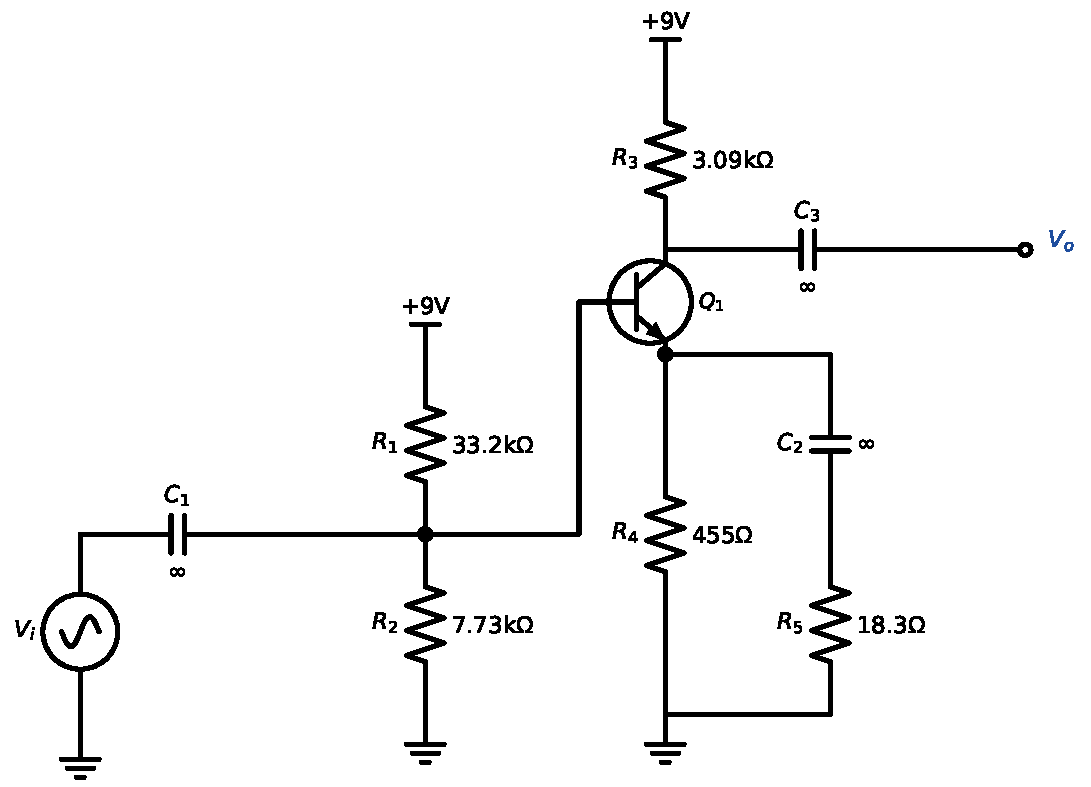
\includegraphics[width=0.9\linewidth,height=6.5cm,keepaspectratio]{p05_designed}\end{center}

\begin{ansbox}
$R_{1} = 33.2\,\mathrm{k}\Omega$,\quad $R_{2} = 7.73\,\mathrm{k}\Omega$,\quad $R_{3} = 3.09\,\mathrm{k}\Omega$,\quad $R_{4} = 455\,\Omega$,\quad $R_{5} = 18.3\,\Omega$
\end{ansbox}

\newpage
\subsection*{Solution 4E.6 \hfill Easy}
\begin{center}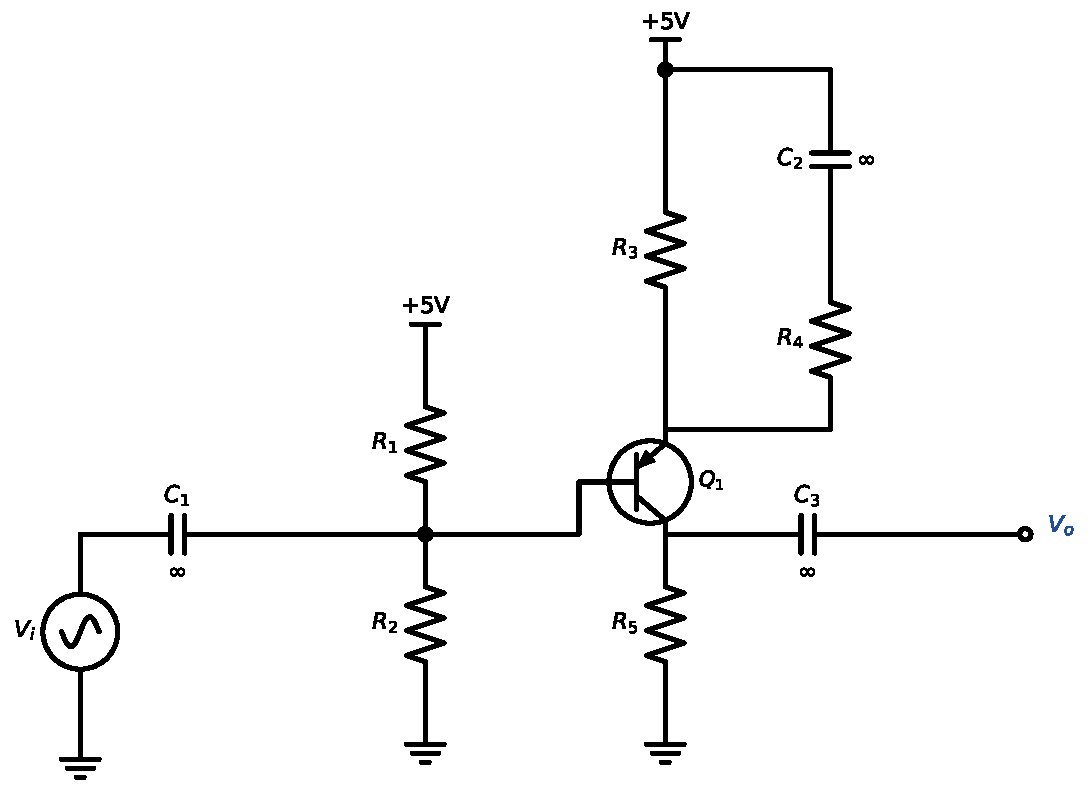
\includegraphics[width=0.9\linewidth,height=6cm,keepaspectratio]{p06_circuit}\end{center}
\solstep{1}{Plan}Name the resistors by their job: $R_{1} = R_{B1}$, $R_{2} = R_{B2}$, $R_{3} = R_{E1}$, $R_{4} = R_{G1}$, $R_{5} = R_{C1}$. Every stage is biased like the one-stage design of the slides: $V_{RE}\ge1$\,V ($V_{BE}$-insensitive), the divider and every collector current much larger than the base current it feeds ($\beta$-insensitive, factor $N$), and $V_{RC}$ as large as the swing allows. Small-signal tools: $r_e = V_T/I_C$, CE gain $|A_v| = \frac{Z_C}{r_e + R_E\|R_G}$, follower gain $\frac{Z_E}{r_e+Z_E}$, base resistance $(\beta+1)(r_e + Z_E)$ (the $\infty$ capacitors put $R_G$ in parallel with $R_E$ for AC only). Design from the output back to the input, because each stage loads the one before it.
\solstep{2}{Output stage}$V_{BE}$-insensitive: $V_{RE1} \ge 1$\,V; use $V_{RE1} = 1$\,V.

To avoid clipping at saturation the collector must be able to swing down by $\hat V_o$ without $V_{CE}$ dropping below $V_{CE,sat}$, and at cutoff $V_{RC}$ must be at least $\hat V_o$: $V_{CC} - \hat V_o - V_{RE1} - V_{CE,sat} \ge V_{RC1} \ge \hat V_o$. Take the largest value (most gain, best linearity): \[V_{RC1} = 5 - 1 - 1 - 0.2 = 2.8\,\mathrm{V} \;\ge\; \hat V_o = 1\,\mathrm{V}\ \checkmark\]

Maximum available gain ($R_G=0$, $R_C$ only): $|A_v|_{max} = \frac{R_C}{r_e} = \frac{V_{RC1}/I_C}{V_T/I_C} = \frac{V_{RC1}}{V_T} = \frac{2.8}{0.025} = 112 \ge 50$ \checkmark
\solstep{3}{Bias current and resistors}Divider: $V_{RB2} = V_{B1} = 3.3\,\mathrm{V}$, $V_{RB1} = V_{CC} - V_{B1} = 1.7\,\mathrm{V}$ ($|V_{RE1}| + 0.7$ on the emitter side). $\beta$-insensitive: the divider current is $N$ times the base current, $I_{RB} = N\frac{I_{C1}}{\beta}$, $N = 10$. Input resistance (all three in parallel, with $(\beta+1)(r_e + R_E\|R_G) \approx \beta\frac{R_{C1}}{|A_{v1}|} = \beta\frac{V_{RC1}}{I_{C1}|A_{v1}|}$):\[R_i \approx \frac{\beta/I_{C1}}{\frac{N}{V_{RB1}} + \frac{N}{V_{RB2}} + \frac{|A_{v1}|}{V_{RC1}}} \ge R_{i,spec} \;\Rightarrow\; I_{C1} \le \frac{\beta/R_{i,spec}}{\frac{10}{1.7} + \frac{10}{3.3} + \frac{50}{2.8}} = 3.74\,\mathrm{m}\mathrm{A}\]Take the E12 value just below: $I_{C1} = 3.3\,\mathrm{m}\mathrm{A}$. 

\[R_{C1} = \frac{V_{RC1}}{I_{C1}} = \frac{2.8}{3.3\,\mathrm{m}\mathrm{A}} = \mathbf{848\,\Omega},\quad R_{E1} = \frac{V_{RE1}}{I_{C1}} = \frac{1}{3.3\,\mathrm{m}\mathrm{A}} = \mathbf{303\,\Omega},\quad r_{e1} = \frac{V_T}{I_{C1}} = 7.58\,\Omega\]

Gain $|A_{v1}| = \frac{R_{C1}}{r_{e1} + R_{E1}\|R_{G1}} = 50$:\[R_{E1}\|R_{G1} = \frac{R_{C1}}{|A_{v1}|} - r_{e1} = 9.39\,\Omega \;\Rightarrow\; R_{G1} = \frac{1}{\frac{1}{9.39\,\Omega} - \frac{1}{303\,\Omega}} = \mathbf{9.69\,\Omega}\]

\[R_{B1} = \frac{V_{RB1}}{N I_{C1}/\beta} = \frac{1.7}{330\,\mu \mathrm{A}} = \mathbf{5.15\,\mathrm{k}\Omega},\qquad R_{B2} = \frac{V_{RB2}}{N I_{C1}/\beta} = \frac{3.3}{330\,\mu \mathrm{A}} = \mathbf{10\,\mathrm{k}\Omega}\]

Check: $R_i = R_{B1}\|R_{B2}\|(\beta+1)(r_{e1} + R_{E1}\|R_{G1}) = 5.15\,\mathrm{k}\Omega\|10\,\mathrm{k}\Omega\|1.71\,\mathrm{k}\Omega = 1.14\,\mathrm{k}\Omega$ $\ge 1\,\mathrm{k}\Omega$ \checkmark.
\solstep{4}{Check by analysis}Solve the finished circuit exactly ($\beta=100$, base currents included) for the DC point, then the small-signal gain with the exact $r_e$ values:\begin{center}\renewcommand{\arraystretch}{1.35}
\begin{tabular}{cccc}
\toprule
 & design $I_C$ & exact $I_C$ & exact $|V_{CE}|$ \\
\midrule
$Q_{1}$ & $3.3\,\mathrm{m}\mathrm{A}$ & $2.94\,\mathrm{m}\mathrm{A}$ & $1.605\,\mathrm{V}$ \\
\bottomrule
\end{tabular}\end{center}
The exact currents are a little off the design values: $N$ only makes each base current $N$ times smaller than the current it disturbs, so the base voltages sag slightly, and along direct-coupled stages each shift is passed on (and amplified) to the next stage. The slides handle this the same way: simulate, then adjust. The exact gain is $|A_v| = 46.94$ instead of $50$ (the hand design ignored $\alpha$ and the base currents). As the slides suggest, trim $R_{G1}$: the gain is proportional to $1/(r_{e1} + R_{E1}\|R_{G1})$, so scale that sum by $46.94/50$ (exact $r_{e1} = 8.5\,\Omega$):\[R_{E1}\|R_{G1} = (8.5\,\Omega + 9.39\,\Omega)\frac{46.94}{50} - 8.5\,\Omega = 8.3\,\Omega \;\Rightarrow\; R_{G1} = \mathbf{8.53\,\Omega}\]Re-analysis: $|A_v| = 50$ \checkmark. \begin{itemize}[leftmargin=*,itemsep=2pt]
\item Input resistance (exact): $R_i = 1.13\,\mathrm{k}\Omega$ $\ge 1\,\mathrm{k}\Omega$ \checkmark
\item Output swing: $Q_{1}$ clips (saturation or cutoff) at $\hat V_o = 1.405\,\mathrm{V}$. The smallest, $1.405\,\mathrm{V}$, is $\ge 1$\,V \checkmark
\item Distortion: each CE stage adds $HD_2 \approx \frac{\hat v_b}{4V_T}\left(\frac{r_e}{r_e + R_E\|R_G}\right)^2$ ($\hat v_b$ = its input amplitude at the specified output; for one stage this is the slides' $\frac{\hat V_o V_T |A_v|}{4V_{RC}^2}$): THD $\approx 4.5\,\%$ $\le 5\,\%$ \checkmark
\item $V_{BE}$-insensitive: $V_{RE1} = 1$\,V $\ge 1$\,V \checkmark
\end{itemize}

\begin{center}\renewcommand{\arraystretch}{1.35}
\begin{tabular}{ll}
\toprule
resistor & value \\
\midrule
$R_{1}$ ($R_{B1}$) & $5.15\,\mathrm{k}\Omega$ \\
$R_{2}$ ($R_{B2}$) & $10\,\mathrm{k}\Omega$ \\
$R_{3}$ ($R_{E1}$) & $303\,\Omega$ \\
$R_{4}$ ($R_{G1}$) & $8.53\,\Omega$ \\
$R_{5}$ ($R_{C1}$) & $848\,\Omega$ \\
\bottomrule
\end{tabular}\end{center}
\begin{center}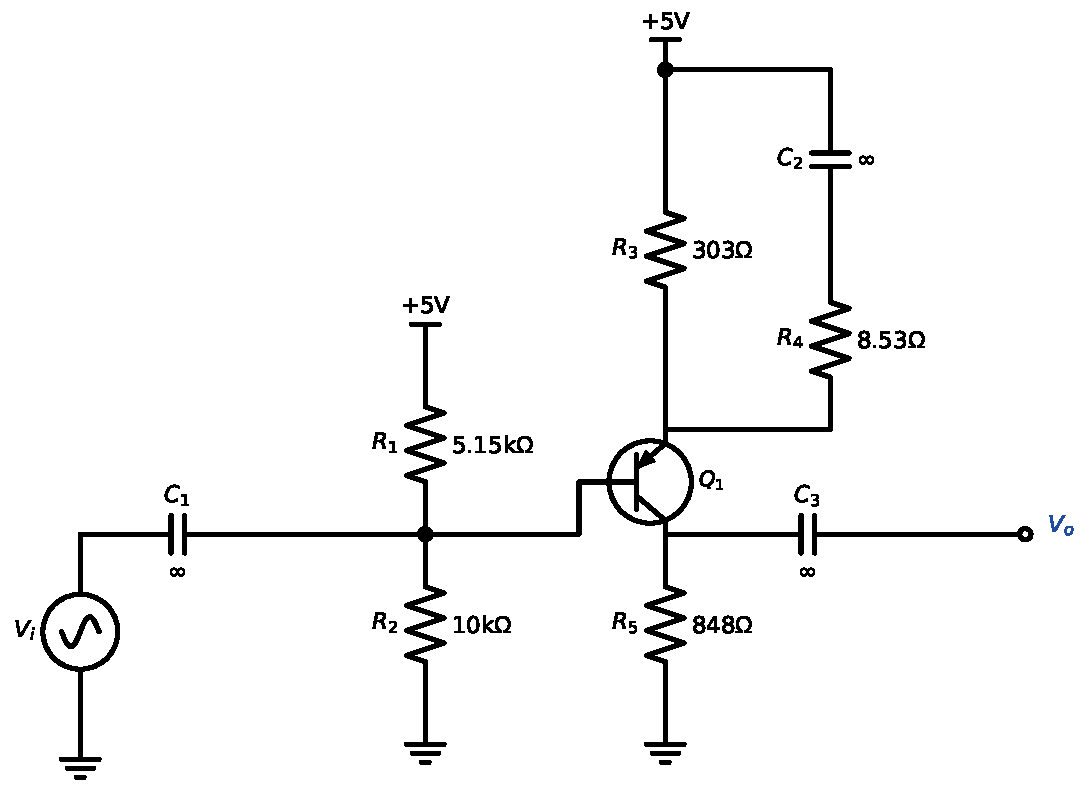
\includegraphics[width=0.9\linewidth,height=6.5cm,keepaspectratio]{p06_designed}\end{center}

\begin{ansbox}
$R_{1} = 5.15\,\mathrm{k}\Omega$,\quad $R_{2} = 10\,\mathrm{k}\Omega$,\quad $R_{3} = 303\,\Omega$,\quad $R_{4} = 8.53\,\Omega$,\quad $R_{5} = 848\,\Omega$
\end{ansbox}

\newpage
\subsection*{Solution 4E.7 \hfill Medium}
\begin{center}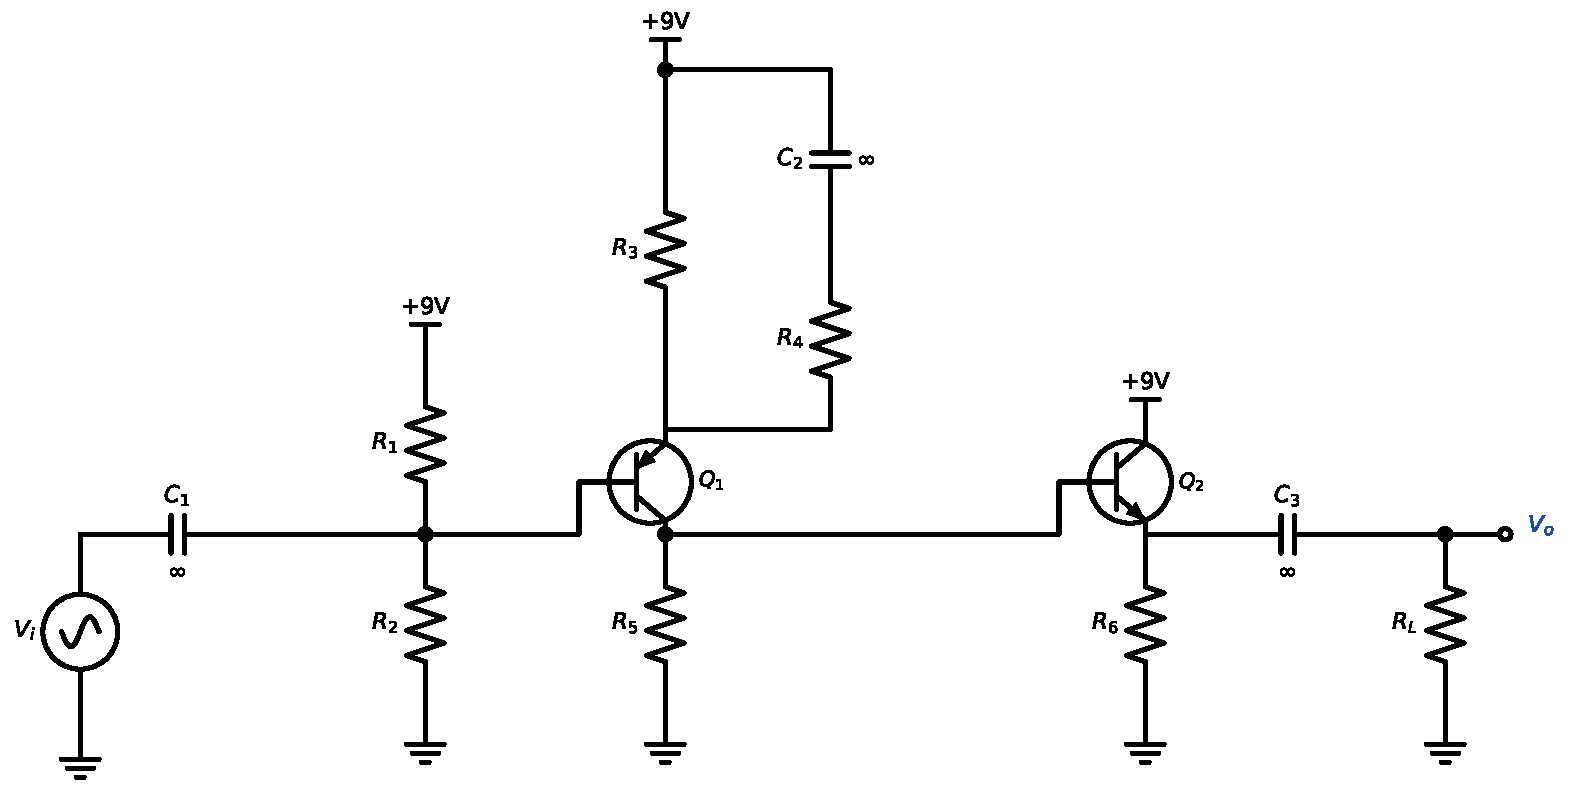
\includegraphics[width=0.9\linewidth,height=6cm,keepaspectratio]{p07_circuit}\end{center}
\solstep{1}{Plan}Name the resistors by their job: $R_{1} = R_{B1}$, $R_{2} = R_{B2}$, $R_{3} = R_{E1}$, $R_{4} = R_{G1}$, $R_{5} = R_{C1}$, $R_{6} = R_H$. Every stage is biased like the one-stage design of the slides: $V_{RE}\ge1$\,V ($V_{BE}$-insensitive), the divider and every collector current much larger than the base current it feeds ($\beta$-insensitive, factor $N$), and $V_{RC}$ as large as the swing allows. Small-signal tools: $r_e = V_T/I_C$, CE gain $|A_v| = \frac{Z_C}{r_e + R_E\|R_G}$, follower gain $\frac{Z_E}{r_e+Z_E}$, base resistance $(\beta+1)(r_e + Z_E)$ (the $\infty$ capacitors put $R_G$ in parallel with $R_E$ for AC only). Design from the output back to the input, because each stage loads the one before it.
\solstep{2}{Output stage and follower}$V_{BE}$-insensitive: $V_{RE1} \ge 1$\,V; use $V_{RE1} = 1$\,V.

To avoid clipping at saturation the collector must be able to swing down by $\hat V_o$ without $V_{CE}$ dropping below $V_{CE,sat}$, and at cutoff $V_{RC}$ must be at least $\hat V_o$: $V_{CC} - \hat V_o - V_{RE1} - V_{CE,sat} \ge V_{RC1} \ge \hat V_o$. Take the largest value (most gain, best linearity): \[V_{RC1} = 9 - 1.8 - 1 - 0.2 = 6\,\mathrm{V} \;\ge\; \hat V_o = 1.8\,\mathrm{V}\ \checkmark\]

Maximum available gain ($R_G=0$, $R_C$ only): $|A_v|_{max} = \frac{R_C}{r_e} = \frac{V_{RC1}/I_C}{V_T/I_C} = \frac{V_{RC1}}{V_T} = \frac{6}{0.025} = 240 \ge 40$ \checkmark

Follower $Q_{2}$: its emitter sits at $0.7$\,V from the collector of $Q_{1}$, so $V_{RH} = V_{RC1} - 0.7 = 5.3\,\mathrm{V}$. To avoid current clipping the DC current in $R_H$ must stay larger than the peak current pushed into $R_L$: \[\frac{V_{RC1} - 0.7 - \hat V_o}{R_H} \ge \frac{\hat V_o}{R_L} \Rightarrow R_H \le R_L\frac{V_{RC1} - 0.7 - \hat V_o}{\hat V_o} = 500\,\Omega\cdot\frac{5.3 - 1.8}{1.8} = 972\,\Omega\]Take the E12 value just below: $R_H = \mathbf{820\,\Omega}$. Then $I_{C2} \approx \frac{V_{RH}}{R_H} = \frac{5.3}{820\,\Omega} = 6.46\,\mathrm{m}\mathrm{A}$, $r_{e2} = \frac{V_T}{I_{C2}} = 3.87\,\Omega$, and with $R_H \| R_L = 311\,\Omega$:\[A_{v2} = \frac{R_H\|R_L}{r_{e2} + R_H\|R_L} = 0.9877,\qquad R_{i2} = (\beta+1)(r_{e2} + R_H\|R_L) = 31.8\,\mathrm{k}\Omega\]
\solstep{3}{Bias current and resistors}Divider: $V_{RB2} = V_{B1} = 7.3\,\mathrm{V}$, $V_{RB1} = V_{CC} - V_{B1} = 1.7\,\mathrm{V}$ ($|V_{RE1}| + 0.7$ on the emitter side). $\beta$-insensitive: the divider current is $N$ times the base current, $I_{RB} = N\frac{I_{C1}}{\beta}$, $N = 10$. Input resistance (all three in parallel, with $(\beta+1)(r_e + R_E\|R_G) \approx \beta\frac{R_{C1}}{|A_{v1}|} = \beta\frac{V_{RC1}}{I_{C1}|A_{v1}|}$):\[R_i \approx \frac{\beta/I_{C1}}{\frac{N}{V_{RB1}} + \frac{N}{V_{RB2}} + \frac{|A_{v1}|}{V_{RC1}}} \ge R_{i,spec} \;\Rightarrow\; I_{C1} \le \frac{\beta/R_{i,spec}}{\frac{10}{1.7} + \frac{10}{7.3} + \frac{40.5}{6}} = 1.79\,\mathrm{m}\mathrm{A}\]Take the E12 value just below: $I_{C1} = 1.5\,\mathrm{m}\mathrm{A}$. 

\[R_{C1} = \frac{V_{RC1}}{I_{C1}} = \frac{6}{1.5\,\mathrm{m}\mathrm{A}} = \mathbf{4\,\mathrm{k}\Omega},\quad R_{E1} = \frac{V_{RE1}}{I_{C1}} = \frac{1}{1.5\,\mathrm{m}\mathrm{A}} = \mathbf{667\,\Omega},\quad r_{e1} = \frac{V_T}{I_{C1}} = 16.7\,\Omega\]

Gain $|A_{v1}| = \frac{R_{C1}\|R_{i2}}{r_{e1} + R_{E1}\|R_{G1}} = 40.5$ with $R_{C1}\|R_{i2} = 3.55\,\mathrm{k}\Omega$:\[R_{E1}\|R_{G1} = \frac{R_{C1}\|R_{i2}}{|A_{v1}|} - r_{e1} = 71.1\,\Omega \;\Rightarrow\; R_{G1} = \frac{1}{\frac{1}{71.1\,\Omega} - \frac{1}{667\,\Omega}} = \mathbf{79.5\,\Omega}\]

\[R_{B1} = \frac{V_{RB1}}{N I_{C1}/\beta} = \frac{1.7}{150\,\mu \mathrm{A}} = \mathbf{11.3\,\mathrm{k}\Omega},\qquad R_{B2} = \frac{V_{RB2}}{N I_{C1}/\beta} = \frac{7.3}{150\,\mu \mathrm{A}} = \mathbf{48.7\,\mathrm{k}\Omega}\]

Check: $R_i = R_{B1}\|R_{B2}\|(\beta+1)(r_{e1} + R_{E1}\|R_{G1}) = 11.3\,\mathrm{k}\Omega\|48.7\,\mathrm{k}\Omega\|8.86\,\mathrm{k}\Omega = 4.512\,\mathrm{k}\Omega$ $\ge 4\,\mathrm{k}\Omega$ \checkmark.
\solstep{4}{Check by analysis}Solve the finished circuit exactly ($\beta=100$, base currents included) for the DC point, then the small-signal gain with the exact $r_e$ values:\begin{center}\renewcommand{\arraystretch}{1.35}
\begin{tabular}{cccc}
\toprule
 & design $I_C$ & exact $I_C$ & exact $|V_{CE}|$ \\
\midrule
$Q_{1}$ & $1.5\,\mathrm{m}\mathrm{A}$ & $1.31\,\mathrm{m}\mathrm{A}$ & $3.102\,\mathrm{V}$ \\
$Q_{2}$ & $6.46\,\mathrm{m}\mathrm{A}$ & $5.21\,\mathrm{m}\mathrm{A}$ & $4.682\,\mathrm{V}$ \\
\bottomrule
\end{tabular}\end{center}
The exact currents are a little off the design values: $N$ only makes each base current $N$ times smaller than the current it disturbs, so the base voltages sag slightly, and along direct-coupled stages each shift is passed on (and amplified) to the next stage. The slides handle this the same way: simulate, then adjust. The exact gain is $|A_v| = 38.42$ instead of $40$ (the hand design ignored $\alpha$ and the base currents). As the slides suggest, trim $R_{G1}$: the gain is proportional to $1/(r_{e1} + R_{E1}\|R_{G1})$, so scale that sum by $38.42/40$ (exact $r_{e1} = 19.1\,\Omega$):\[R_{E1}\|R_{G1} = (19.1\,\Omega + 71.1\,\Omega)\frac{38.42}{40} - 19.1\,\Omega = 67.5\,\Omega \;\Rightarrow\; R_{G1} = \mathbf{75.1\,\Omega}\]Re-analysis: $|A_v| = 40$ \checkmark. \begin{itemize}[leftmargin=*,itemsep=2pt]
\item Input resistance (exact): $R_i = 4.48\,\mathrm{k}\Omega$ $\ge 4\,\mathrm{k}\Omega$ \checkmark
\item Output swing: follower current clipping at $\hat V_o = I_{E2}(R_H\|R_L) = 1.62\,\mathrm{V}$; $Q_{1}$ clips (saturation or cutoff) at $\hat V_o = 2.858\,\mathrm{V}$. The smallest, $1.62\,\mathrm{V}$, is $\ge 1.5$\,V \checkmark
\item Distortion: each CE stage adds $HD_2 \approx \frac{\hat v_b}{4V_T}\left(\frac{r_e}{r_e + R_E\|R_G}\right)^2$ ($\hat v_b$ = its input amplitude at the specified output; for one stage this is the slides' $\frac{\hat V_o V_T |A_v|}{4V_{RC}^2}$): THD $\approx 1.7\,\%$ $\le 3\,\%$ \checkmark
\item $V_{BE}$-insensitive: $V_{RE1} = 1$\,V $\ge 1$\,V \checkmark
\end{itemize}

\begin{center}\renewcommand{\arraystretch}{1.35}
\begin{tabular}{ll}
\toprule
resistor & value \\
\midrule
$R_{1}$ ($R_{B1}$) & $11.3\,\mathrm{k}\Omega$ \\
$R_{2}$ ($R_{B2}$) & $48.7\,\mathrm{k}\Omega$ \\
$R_{3}$ ($R_{E1}$) & $667\,\Omega$ \\
$R_{4}$ ($R_{G1}$) & $75.1\,\Omega$ \\
$R_{5}$ ($R_{C1}$) & $4\,\mathrm{k}\Omega$ \\
$R_{6}$ ($R_H$) & $820\,\Omega$ \\
\bottomrule
\end{tabular}\end{center}
\begin{center}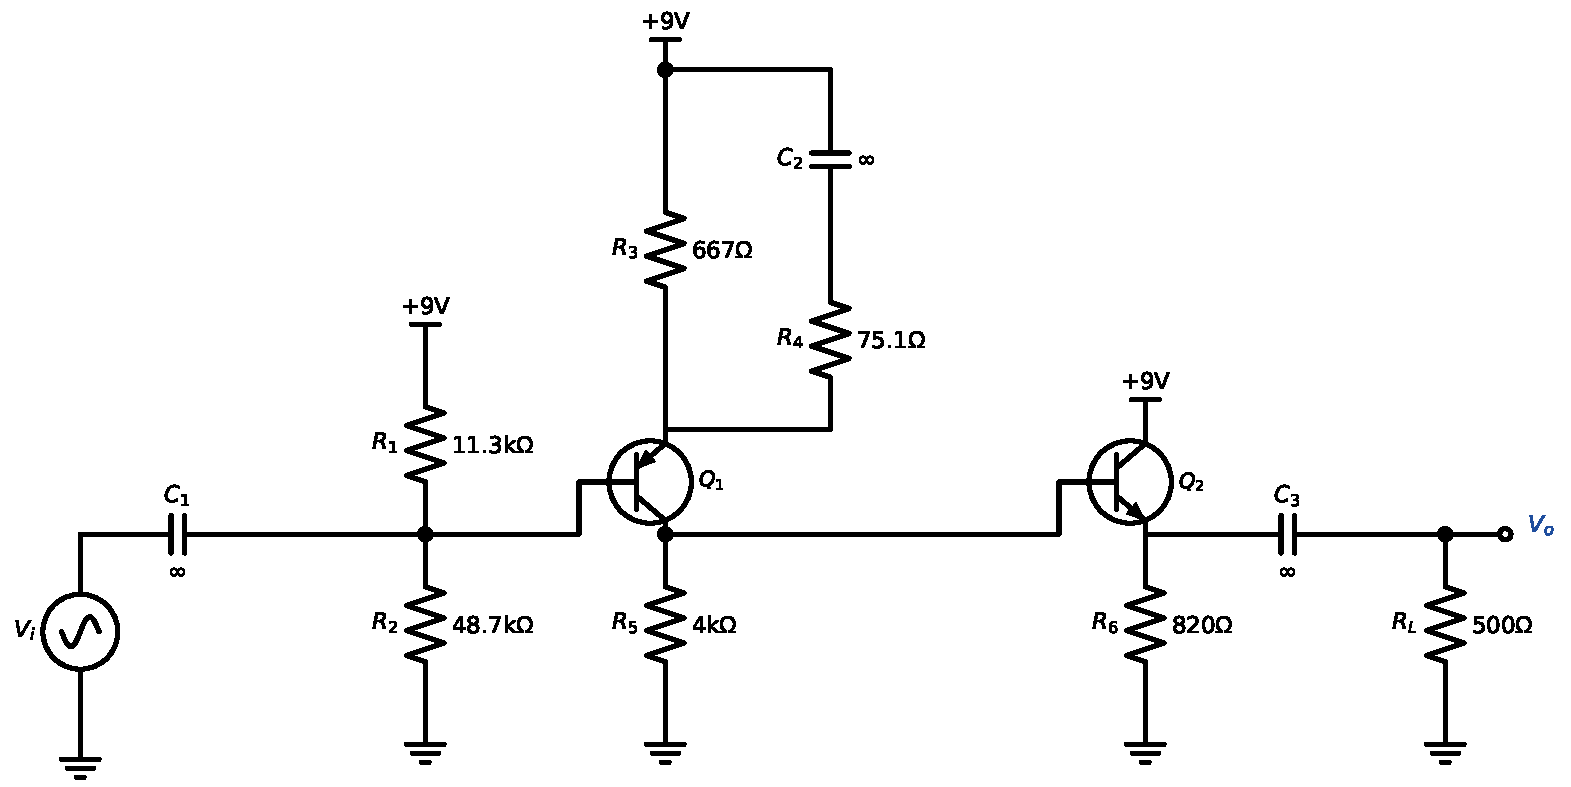
\includegraphics[width=0.9\linewidth,height=6.5cm,keepaspectratio]{p07_designed}\end{center}

\begin{ansbox}
$R_{1} = 11.3\,\mathrm{k}\Omega$,\quad $R_{2} = 48.7\,\mathrm{k}\Omega$,\quad $R_{3} = 667\,\Omega$,\quad $R_{4} = 75.1\,\Omega$,\quad $R_{5} = 4\,\mathrm{k}\Omega$,\quad $R_{6} = 820\,\Omega$
\end{ansbox}

\newpage
\subsection*{Solution 4E.8 \hfill Medium}
\begin{center}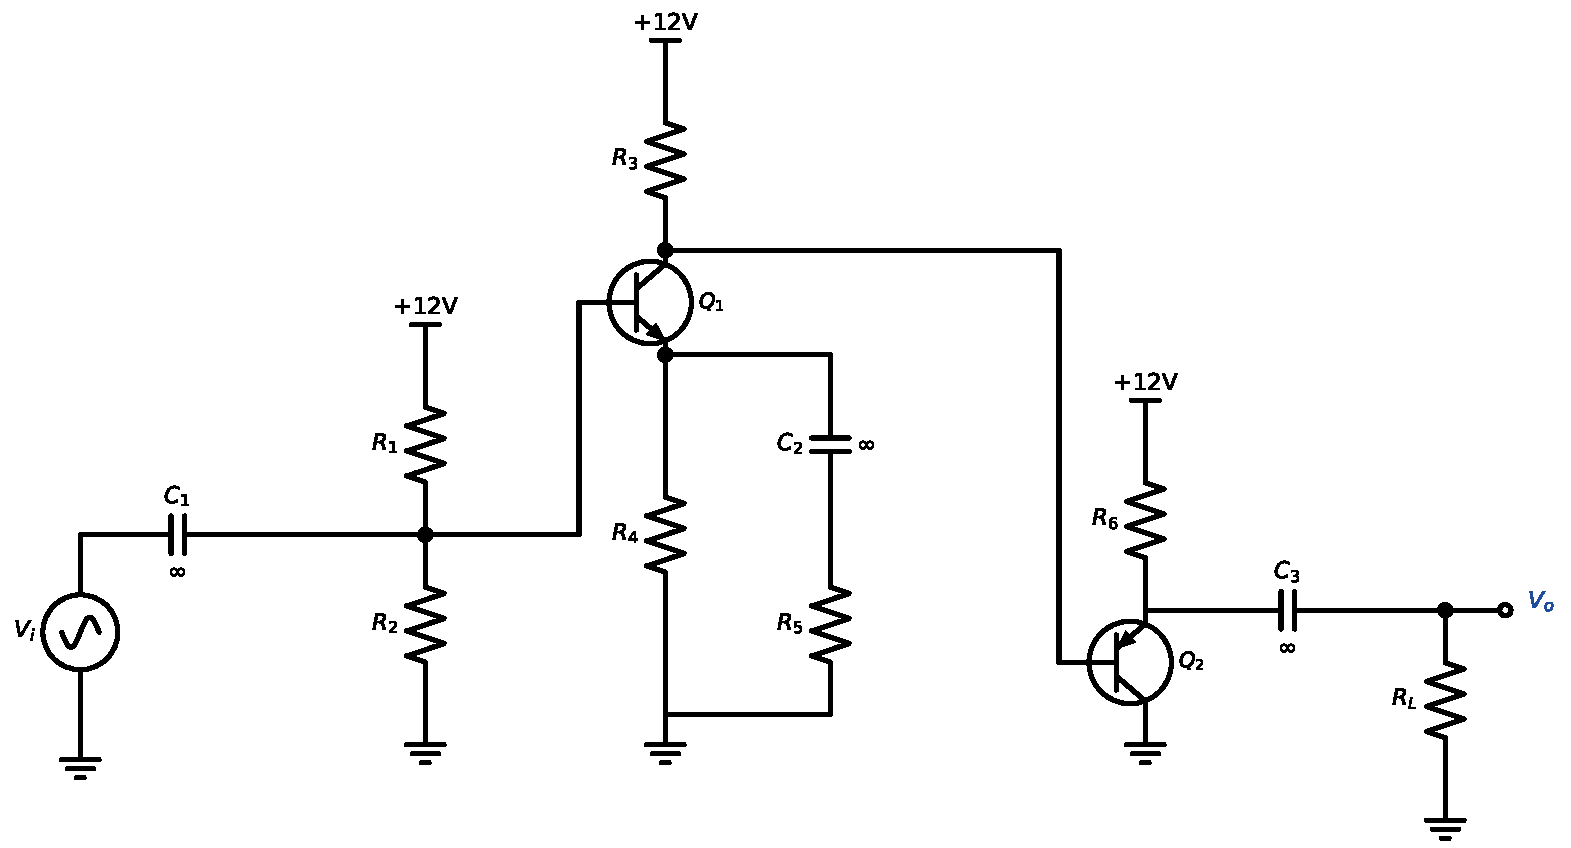
\includegraphics[width=0.9\linewidth,height=6cm,keepaspectratio]{p08_circuit}\end{center}
\solstep{1}{Plan}Name the resistors by their job: $R_{1} = R_{B1}$, $R_{2} = R_{B2}$, $R_{3} = R_{C1}$, $R_{4} = R_{E1}$, $R_{5} = R_{G1}$, $R_{6} = R_H$. Every stage is biased like the one-stage design of the slides: $V_{RE}\ge1$\,V ($V_{BE}$-insensitive), the divider and every collector current much larger than the base current it feeds ($\beta$-insensitive, factor $N$), and $V_{RC}$ as large as the swing allows. Small-signal tools: $r_e = V_T/I_C$, CE gain $|A_v| = \frac{Z_C}{r_e + R_E\|R_G}$, follower gain $\frac{Z_E}{r_e+Z_E}$, base resistance $(\beta+1)(r_e + Z_E)$ (the $\infty$ capacitors put $R_G$ in parallel with $R_E$ for AC only). Design from the output back to the input, because each stage loads the one before it.
\solstep{2}{Output stage and follower}$V_{BE}$-insensitive: $V_{RE1} \ge 1$\,V; use $V_{RE1} = 1$\,V.

To avoid clipping at saturation the collector must be able to swing down by $\hat V_o$ without $V_{CE}$ dropping below $V_{CE,sat}$, and at cutoff $V_{RC}$ must be at least $\hat V_o$: $V_{CC} - \hat V_o - V_{RE1} - V_{CE,sat} \ge V_{RC1} \ge \hat V_o$. Take the largest value (most gain, best linearity): \[V_{RC1} = 12 - 2.4 - 1 - 0.2 = 8.4\,\mathrm{V} \;\ge\; \hat V_o = 2.4\,\mathrm{V}\ \checkmark\]

Maximum available gain ($R_G=0$, $R_C$ only): $|A_v|_{max} = \frac{R_C}{r_e} = \frac{V_{RC1}/I_C}{V_T/I_C} = \frac{V_{RC1}}{V_T} = \frac{8.4}{0.025} = 336 \ge 60$ \checkmark

Follower $Q_{2}$: its emitter sits at $0.7$\,V from the collector of $Q_{1}$, so $V_{RH} = V_{RC1} - 0.7 = 7.7\,\mathrm{V}$. To avoid current clipping the DC current in $R_H$ must stay larger than the peak current pushed into $R_L$: \[\frac{V_{RC1} - 0.7 - \hat V_o}{R_H} \ge \frac{\hat V_o}{R_L} \Rightarrow R_H \le R_L\frac{V_{RC1} - 0.7 - \hat V_o}{\hat V_o} = 1\,\mathrm{k}\Omega\cdot\frac{7.7 - 2.4}{2.4} = 2.21\,\mathrm{k}\Omega\]Take the E12 value just below: $R_H = \mathbf{2.2\,\mathrm{k}\Omega}$. Then $I_{C2} \approx \frac{V_{RH}}{R_H} = \frac{7.7}{2.2\,\mathrm{k}\Omega} = 3.5\,\mathrm{m}\mathrm{A}$, $r_{e2} = \frac{V_T}{I_{C2}} = 7.14\,\Omega$, and with $R_H \| R_L = 688\,\Omega$:\[A_{v2} = \frac{R_H\|R_L}{r_{e2} + R_H\|R_L} = 0.9897,\qquad R_{i2} = (\beta+1)(r_{e2} + R_H\|R_L) = 70.2\,\mathrm{k}\Omega\]
\solstep{3}{Bias current and resistors}Divider: $V_{RB2} = V_{B1} = 1.7\,\mathrm{V}$, $V_{RB1} = V_{CC} - V_{B1} = 10.3\,\mathrm{V}$ ($|V_{RE1}| + 0.7$ on the emitter side). $\beta$-insensitive: the divider current is $N$ times the base current, $I_{RB} = N\frac{I_{C1}}{\beta}$, $N = 10$. Input resistance (all three in parallel, with $(\beta+1)(r_e + R_E\|R_G) \approx \beta\frac{R_{C1}}{|A_{v1}|} = \beta\frac{V_{RC1}}{I_{C1}|A_{v1}|}$):\[R_i \approx \frac{\beta/I_{C1}}{\frac{N}{V_{RB1}} + \frac{N}{V_{RB2}} + \frac{|A_{v1}|}{V_{RC1}}} \ge R_{i,spec} \;\Rightarrow\; I_{C1} \le \frac{\beta/R_{i,spec}}{\frac{10}{10.3} + \frac{10}{1.7} + \frac{60.62}{8.4}} = 1.42\,\mathrm{m}\mathrm{A}\]Take the E12 value just below: $I_{C1} = 1.2\,\mathrm{m}\mathrm{A}$. 

\[R_{C1} = \frac{V_{RC1}}{I_{C1}} = \frac{8.4}{1.2\,\mathrm{m}\mathrm{A}} = \mathbf{7\,\mathrm{k}\Omega},\quad R_{E1} = \frac{V_{RE1}}{I_{C1}} = \frac{1}{1.2\,\mathrm{m}\mathrm{A}} = \mathbf{833\,\Omega},\quad r_{e1} = \frac{V_T}{I_{C1}} = 20.8\,\Omega\]

Gain $|A_{v1}| = \frac{R_{C1}\|R_{i2}}{r_{e1} + R_{E1}\|R_{G1}} = 60.62$ with $R_{C1}\|R_{i2} = 6.36\,\mathrm{k}\Omega$:\[R_{E1}\|R_{G1} = \frac{R_{C1}\|R_{i2}}{|A_{v1}|} - r_{e1} = 84.2\,\Omega \;\Rightarrow\; R_{G1} = \frac{1}{\frac{1}{84.2\,\Omega} - \frac{1}{833\,\Omega}} = \mathbf{93.6\,\Omega}\]

\[R_{B1} = \frac{V_{RB1}}{N I_{C1}/\beta} = \frac{10.3}{120\,\mu \mathrm{A}} = \mathbf{85.8\,\mathrm{k}\Omega},\qquad R_{B2} = \frac{V_{RB2}}{N I_{C1}/\beta} = \frac{1.7}{120\,\mu \mathrm{A}} = \mathbf{14.2\,\mathrm{k}\Omega}\]

Check: $R_i = R_{B1}\|R_{B2}\|(\beta+1)(r_{e1} + R_{E1}\|R_{G1}) = 85.8\,\mathrm{k}\Omega\|14.2\,\mathrm{k}\Omega\|10.6\,\mathrm{k}\Omega = 5.664\,\mathrm{k}\Omega$ $\ge 5\,\mathrm{k}\Omega$ \checkmark.
\solstep{4}{Check by analysis}Solve the finished circuit exactly ($\beta=100$, base currents included) for the DC point, then the small-signal gain with the exact $r_e$ values:\begin{center}\renewcommand{\arraystretch}{1.35}
\begin{tabular}{cccc}
\toprule
 & design $I_C$ & exact $I_C$ & exact $|V_{CE}|$ \\
\midrule
$Q_{1}$ & $1.2\,\mathrm{m}\mathrm{A}$ & $1.04\,\mathrm{m}\mathrm{A}$ & $4.06\,\mathrm{V}$ \\
$Q_{2}$ & $3.5\,\mathrm{m}\mathrm{A}$ & $2.87\,\mathrm{m}\mathrm{A}$ & $5.634\,\mathrm{V}$ \\
\bottomrule
\end{tabular}\end{center}
The exact currents are a little off the design values: $N$ only makes each base current $N$ times smaller than the current it disturbs, so the base voltages sag slightly, and along direct-coupled stages each shift is passed on (and amplified) to the next stage. The slides handle this the same way: simulate, then adjust. The exact gain is $|A_v| = 57.5$ instead of $60$ (the hand design ignored $\alpha$ and the base currents). As the slides suggest, trim $R_{G1}$: the gain is proportional to $1/(r_{e1} + R_{E1}\|R_{G1})$, so scale that sum by $57.5/60$ (exact $r_{e1} = 24.1\,\Omega$):\[R_{E1}\|R_{G1} = (24.1\,\Omega + 84.2\,\Omega)\frac{57.5}{60} - 24.1\,\Omega = 79.7\,\Omega \;\Rightarrow\; R_{G1} = \mathbf{88.1\,\Omega}\]Re-analysis: $|A_v| = 60$ \checkmark. \par The follower would clip at $\hat V_o = I_{E2}(R_H\|R_L) = 2.87\,\mathrm{m}\mathrm{A}\times688\,\Omega = 1.97\,\mathrm{V} < 2$\,V: its exact current is below the design value because the base currents shift the DC voltages along the direct-coupled chain. Adjust: lower $R_H$ to the next E12 value, $R_H = \mathbf{1.8\,\mathrm{k}\Omega}$ (more follower current), and analyse again. The exact gain is $|A_v| = 59.71$, within $0.5\,\%$ of the specification \checkmark. \begin{itemize}[leftmargin=*,itemsep=2pt]
\item Input resistance (exact): $R_i = 5.63\,\mathrm{k}\Omega$ $\ge 5\,\mathrm{k}\Omega$ \checkmark
\item Output swing: follower current clipping at $\hat V_o = I_{E2}(R_H\|R_L) = 2.391\,\mathrm{V}$; $Q_{1}$ clips (saturation or cutoff) at $\hat V_o = 3.862\,\mathrm{V}$. The smallest, $2.391\,\mathrm{V}$, is $\ge 2$\,V \checkmark
\item Distortion: each CE stage adds $HD_2 \approx \frac{\hat v_b}{4V_T}\left(\frac{r_e}{r_e + R_E\|R_G}\right)^2$ ($\hat v_b$ = its input amplitude at the specified output; for one stage this is the slides' $\frac{\hat V_o V_T |A_v|}{4V_{RC}^2}$): THD $\approx 1.7\,\%$ $\le 3\,\%$ \checkmark
\item $V_{BE}$-insensitive: $V_{RE1} = 1$\,V $\ge 1$\,V \checkmark
\end{itemize}

\begin{center}\renewcommand{\arraystretch}{1.35}
\begin{tabular}{ll}
\toprule
resistor & value \\
\midrule
$R_{1}$ ($R_{B1}$) & $85.8\,\mathrm{k}\Omega$ \\
$R_{2}$ ($R_{B2}$) & $14.2\,\mathrm{k}\Omega$ \\
$R_{3}$ ($R_{C1}$) & $7\,\mathrm{k}\Omega$ \\
$R_{4}$ ($R_{E1}$) & $833\,\Omega$ \\
$R_{5}$ ($R_{G1}$) & $88.1\,\Omega$ \\
$R_{6}$ ($R_H$) & $1.8\,\mathrm{k}\Omega$ \\
\bottomrule
\end{tabular}\end{center}
\begin{center}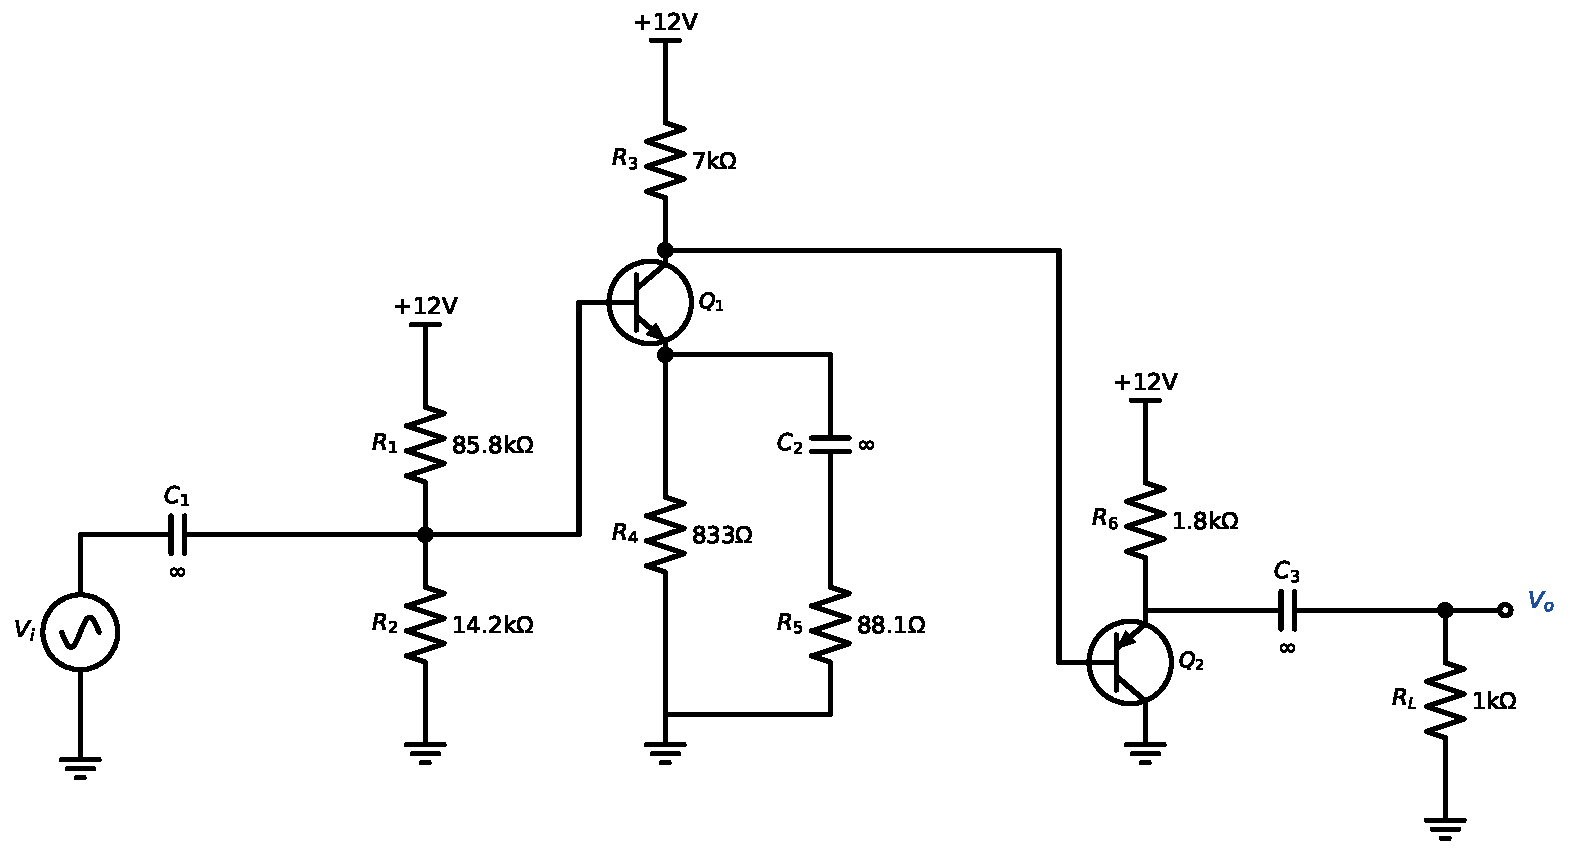
\includegraphics[width=0.9\linewidth,height=6.5cm,keepaspectratio]{p08_designed}\end{center}

\begin{ansbox}
$R_{1} = 85.8\,\mathrm{k}\Omega$,\quad $R_{2} = 14.2\,\mathrm{k}\Omega$,\quad $R_{3} = 7\,\mathrm{k}\Omega$,\quad $R_{4} = 833\,\Omega$,\quad $R_{5} = 88.1\,\Omega$,\quad $R_{6} = 1.8\,\mathrm{k}\Omega$
\end{ansbox}

\newpage
\subsection*{Solution 4E.9 \hfill Medium}
\begin{center}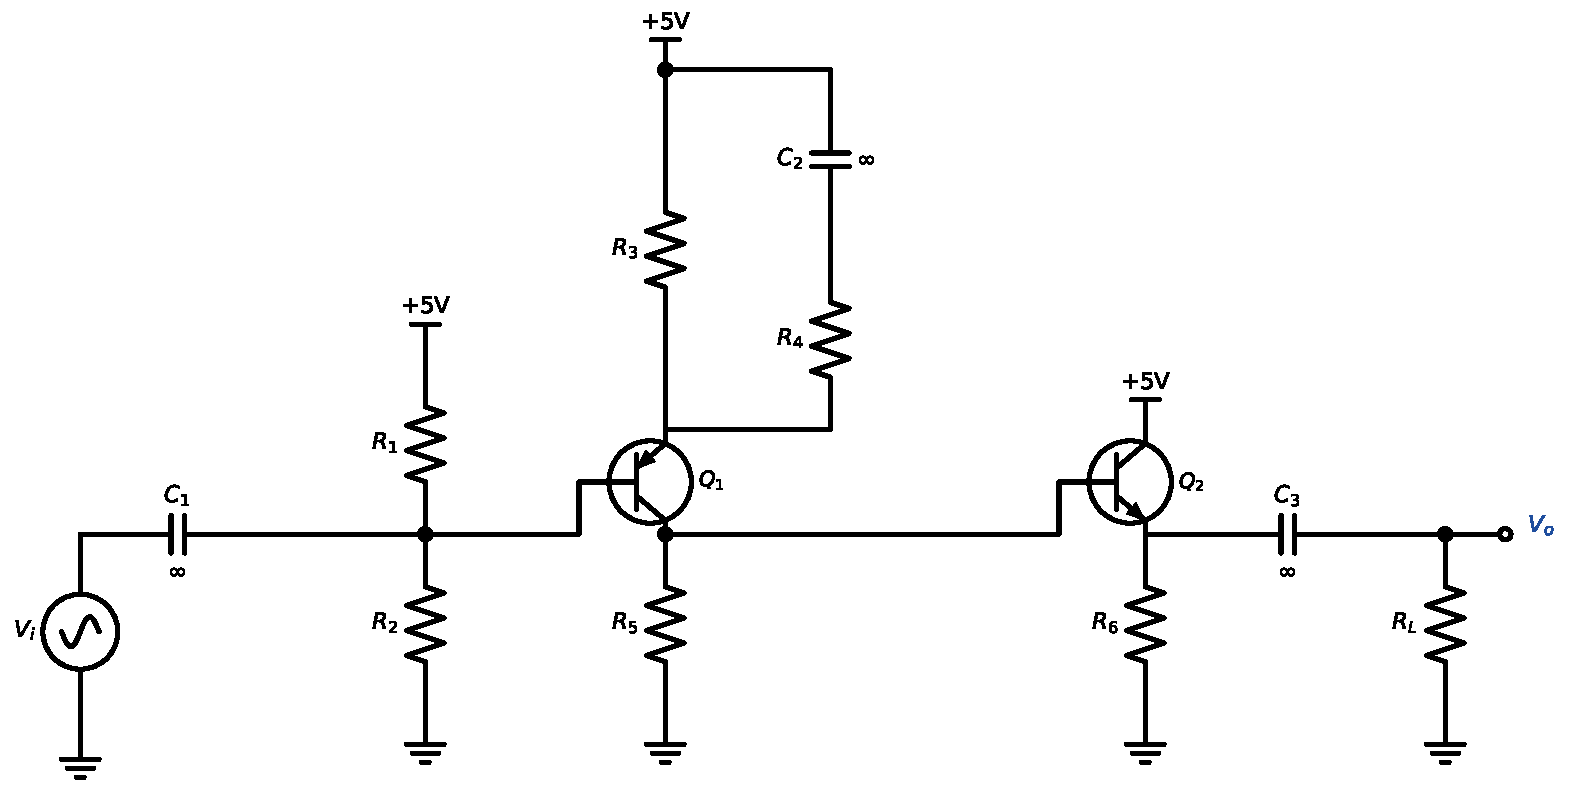
\includegraphics[width=0.9\linewidth,height=6cm,keepaspectratio]{p09_circuit}\end{center}
\solstep{1}{Plan}Name the resistors by their job: $R_{1} = R_{B1}$, $R_{2} = R_{B2}$, $R_{3} = R_{E1}$, $R_{4} = R_{G1}$, $R_{5} = R_{C1}$, $R_{6} = R_H$. Every stage is biased like the one-stage design of the slides: $V_{RE}\ge1$\,V ($V_{BE}$-insensitive), the divider and every collector current much larger than the base current it feeds ($\beta$-insensitive, factor $N$), and $V_{RC}$ as large as the swing allows. Small-signal tools: $r_e = V_T/I_C$, CE gain $|A_v| = \frac{Z_C}{r_e + R_E\|R_G}$, follower gain $\frac{Z_E}{r_e+Z_E}$, base resistance $(\beta+1)(r_e + Z_E)$ (the $\infty$ capacitors put $R_G$ in parallel with $R_E$ for AC only). Design from the output back to the input, because each stage loads the one before it.
\solstep{2}{Output stage and follower}$V_{BE}$-insensitive: $V_{RE1} \ge 1$\,V; use $V_{RE1} = 1$\,V.

To avoid clipping at saturation the collector must be able to swing down by $\hat V_o$ without $V_{CE}$ dropping below $V_{CE,sat}$, and at cutoff $V_{RC}$ must be at least $\hat V_o$: $V_{CC} - \hat V_o - V_{RE1} - V_{CE,sat} \ge V_{RC1} \ge \hat V_o$. Take the largest value (most gain, best linearity): \[V_{RC1} = 5 - 1.2 - 1 - 0.2 = 2.6\,\mathrm{V} \;\ge\; \hat V_o = 1.2\,\mathrm{V}\ \checkmark\]

Maximum available gain ($R_G=0$, $R_C$ only): $|A_v|_{max} = \frac{R_C}{r_e} = \frac{V_{RC1}/I_C}{V_T/I_C} = \frac{V_{RC1}}{V_T} = \frac{2.6}{0.025} = 104 \ge 30$ \checkmark

Follower $Q_{2}$: its emitter sits at $0.7$\,V from the collector of $Q_{1}$, so $V_{RH} = V_{RC1} - 0.7 = 1.9\,\mathrm{V}$. To avoid current clipping the DC current in $R_H$ must stay larger than the peak current pushed into $R_L$: \[\frac{V_{RC1} - 0.7 - \hat V_o}{R_H} \ge \frac{\hat V_o}{R_L} \Rightarrow R_H \le R_L\frac{V_{RC1} - 0.7 - \hat V_o}{\hat V_o} = 200\,\Omega\cdot\frac{1.9 - 1.2}{1.2} = 117\,\Omega\]Take the E12 value just below: $R_H = \mathbf{100\,\Omega}$. Then $I_{C2} \approx \frac{V_{RH}}{R_H} = \frac{1.9}{100\,\Omega} = 19\,\mathrm{m}\mathrm{A}$, $r_{e2} = \frac{V_T}{I_{C2}} = 1.32\,\Omega$, and with $R_H \| R_L = 66.7\,\Omega$:\[A_{v2} = \frac{R_H\|R_L}{r_{e2} + R_H\|R_L} = 0.9806,\qquad R_{i2} = (\beta+1)(r_{e2} + R_H\|R_L) = 6.87\,\mathrm{k}\Omega\]
\solstep{3}{Bias current and resistors}Divider: $V_{RB2} = V_{B1} = 3.3\,\mathrm{V}$, $V_{RB1} = V_{CC} - V_{B1} = 1.7\,\mathrm{V}$ ($|V_{RE1}| + 0.7$ on the emitter side). $\beta$-insensitive: the divider current is $N$ times the base current, $I_{RB} = N\frac{I_{C1}}{\beta}$, $N = 10$. Input resistance (all three in parallel, with $(\beta+1)(r_e + R_E\|R_G) \approx \beta\frac{R_{C1}}{|A_{v1}|} = \beta\frac{V_{RC1}}{I_{C1}|A_{v1}|}$):\[R_i \approx \frac{\beta/I_{C1}}{\frac{N}{V_{RB1}} + \frac{N}{V_{RB2}} + \frac{|A_{v1}|}{V_{RC1}}} \ge R_{i,spec} \;\Rightarrow\; I_{C1} \le \frac{\beta/R_{i,spec}}{\frac{10}{1.7} + \frac{10}{3.3} + \frac{30.59}{2.6}} = 3.22\,\mathrm{m}\mathrm{A}\]Take the E12 value just below: $I_{C1} = 2.7\,\mathrm{m}\mathrm{A}$. 

\[R_{C1} = \frac{V_{RC1}}{I_{C1}} = \frac{2.6}{2.7\,\mathrm{m}\mathrm{A}} = \mathbf{963\,\Omega},\quad R_{E1} = \frac{V_{RE1}}{I_{C1}} = \frac{1}{2.7\,\mathrm{m}\mathrm{A}} = \mathbf{370\,\Omega},\quad r_{e1} = \frac{V_T}{I_{C1}} = 9.26\,\Omega\]

Gain $|A_{v1}| = \frac{R_{C1}\|R_{i2}}{r_{e1} + R_{E1}\|R_{G1}} = 30.59$ with $R_{C1}\|R_{i2} = 845\,\Omega$:\[R_{E1}\|R_{G1} = \frac{R_{C1}\|R_{i2}}{|A_{v1}|} - r_{e1} = 18.3\,\Omega \;\Rightarrow\; R_{G1} = \frac{1}{\frac{1}{18.3\,\Omega} - \frac{1}{370\,\Omega}} = \mathbf{19.3\,\Omega}\]

\[R_{B1} = \frac{V_{RB1}}{N I_{C1}/\beta} = \frac{1.7}{270\,\mu \mathrm{A}} = \mathbf{6.3\,\mathrm{k}\Omega},\qquad R_{B2} = \frac{V_{RB2}}{N I_{C1}/\beta} = \frac{3.3}{270\,\mu \mathrm{A}} = \mathbf{12.2\,\mathrm{k}\Omega}\]

Check: $R_i = R_{B1}\|R_{B2}\|(\beta+1)(r_{e1} + R_{E1}\|R_{G1}) = 6.3\,\mathrm{k}\Omega\|12.2\,\mathrm{k}\Omega\|2.79\,\mathrm{k}\Omega = 1.669\,\mathrm{k}\Omega$ $\ge 1.5\,\mathrm{k}\Omega$ \checkmark.
\solstep{4}{Check by analysis}Solve the finished circuit exactly ($\beta=100$, base currents included) for the DC point, then the small-signal gain with the exact $r_e$ values:\begin{center}\renewcommand{\arraystretch}{1.35}
\begin{tabular}{cccc}
\toprule
 & design $I_C$ & exact $I_C$ & exact $|V_{CE}|$ \\
\midrule
$Q_{1}$ & $2.7\,\mathrm{m}\mathrm{A}$ & $2.41\,\mathrm{m}\mathrm{A}$ & $1.924\,\mathrm{V}$ \\
$Q_{2}$ & $19\,\mathrm{m}\mathrm{A}$ & $14.6\,\mathrm{m}\mathrm{A}$ & $3.524\,\mathrm{V}$ \\
\bottomrule
\end{tabular}\end{center}
The exact currents are a little off the design values: $N$ only makes each base current $N$ times smaller than the current it disturbs, so the base voltages sag slightly, and along direct-coupled stages each shift is passed on (and amplified) to the next stage. The slides handle this the same way: simulate, then adjust. The exact gain is $|A_v| = 28.39$ instead of $30$ (the hand design ignored $\alpha$ and the base currents). As the slides suggest, trim $R_{G1}$: the gain is proportional to $1/(r_{e1} + R_{E1}\|R_{G1})$, so scale that sum by $28.39/30$ (exact $r_{e1} = 10.4\,\Omega$):\[R_{E1}\|R_{G1} = (10.4\,\Omega + 18.3\,\Omega)\frac{28.39}{30} - 10.4\,\Omega = 16.8\,\Omega \;\Rightarrow\; R_{G1} = \mathbf{17.6\,\Omega}\]Re-analysis: $|A_v| = 30$ \checkmark. \par The follower would clip at $\hat V_o = I_{E2}(R_H\|R_L) = 14.6\,\mathrm{m}\mathrm{A}\times66.7\,\Omega = 0.9743\,\mathrm{V} < 1$\,V: its exact current is below the design value because the base currents shift the DC voltages along the direct-coupled chain. Adjust: lower $R_H$ to the next E12 value, $R_H = \mathbf{82\,\Omega}$ (more follower current), and analyse again. The exact gain is $|A_v| = 29.5$ instead of $30$ (the hand design ignored $\alpha$ and the base currents). As the slides suggest, trim $R_{G1}$: the gain is proportional to $1/(r_{e1} + R_{E1}\|R_{G1})$, so scale that sum by $29.5/30$ (exact $r_{e1} = 10.4\,\Omega$):\[R_{E1}\|R_{G1} = (10.4\,\Omega + 16.8\,\Omega)\frac{29.5}{30} - 10.4\,\Omega = 16.3\,\Omega \;\Rightarrow\; R_{G1} = \mathbf{17.1\,\Omega}\]Re-analysis: $|A_v| = 30$ \checkmark. \begin{itemize}[leftmargin=*,itemsep=2pt]
\item Input resistance (exact): $R_i = 1.64\,\mathrm{k}\Omega$ $\ge 1.5\,\mathrm{k}\Omega$ \checkmark
\item Output swing: follower current clipping at $\hat V_o = I_{E2}(R_H\|R_L) = 1.166\,\mathrm{V}$; $Q_{1}$ clips (saturation or cutoff) at $\hat V_o = 1.715\,\mathrm{V}$. The smallest, $1.166\,\mathrm{V}$, is $\ge 1$\,V \checkmark
\item Distortion: each CE stage adds $HD_2 \approx \frac{\hat v_b}{4V_T}\left(\frac{r_e}{r_e + R_E\|R_G}\right)^2$ ($\hat v_b$ = its input amplitude at the specified output; for one stage this is the slides' $\frac{\hat V_o V_T |A_v|}{4V_{RC}^2}$): THD $\approx 4.4\,\%$ $\le 5\,\%$ \checkmark
\item $V_{BE}$-insensitive: $V_{RE1} = 1$\,V $\ge 1$\,V \checkmark
\end{itemize}

\begin{center}\renewcommand{\arraystretch}{1.35}
\begin{tabular}{ll}
\toprule
resistor & value \\
\midrule
$R_{1}$ ($R_{B1}$) & $6.3\,\mathrm{k}\Omega$ \\
$R_{2}$ ($R_{B2}$) & $12.2\,\mathrm{k}\Omega$ \\
$R_{3}$ ($R_{E1}$) & $370\,\Omega$ \\
$R_{4}$ ($R_{G1}$) & $17.1\,\Omega$ \\
$R_{5}$ ($R_{C1}$) & $963\,\Omega$ \\
$R_{6}$ ($R_H$) & $82\,\Omega$ \\
\bottomrule
\end{tabular}\end{center}
\begin{center}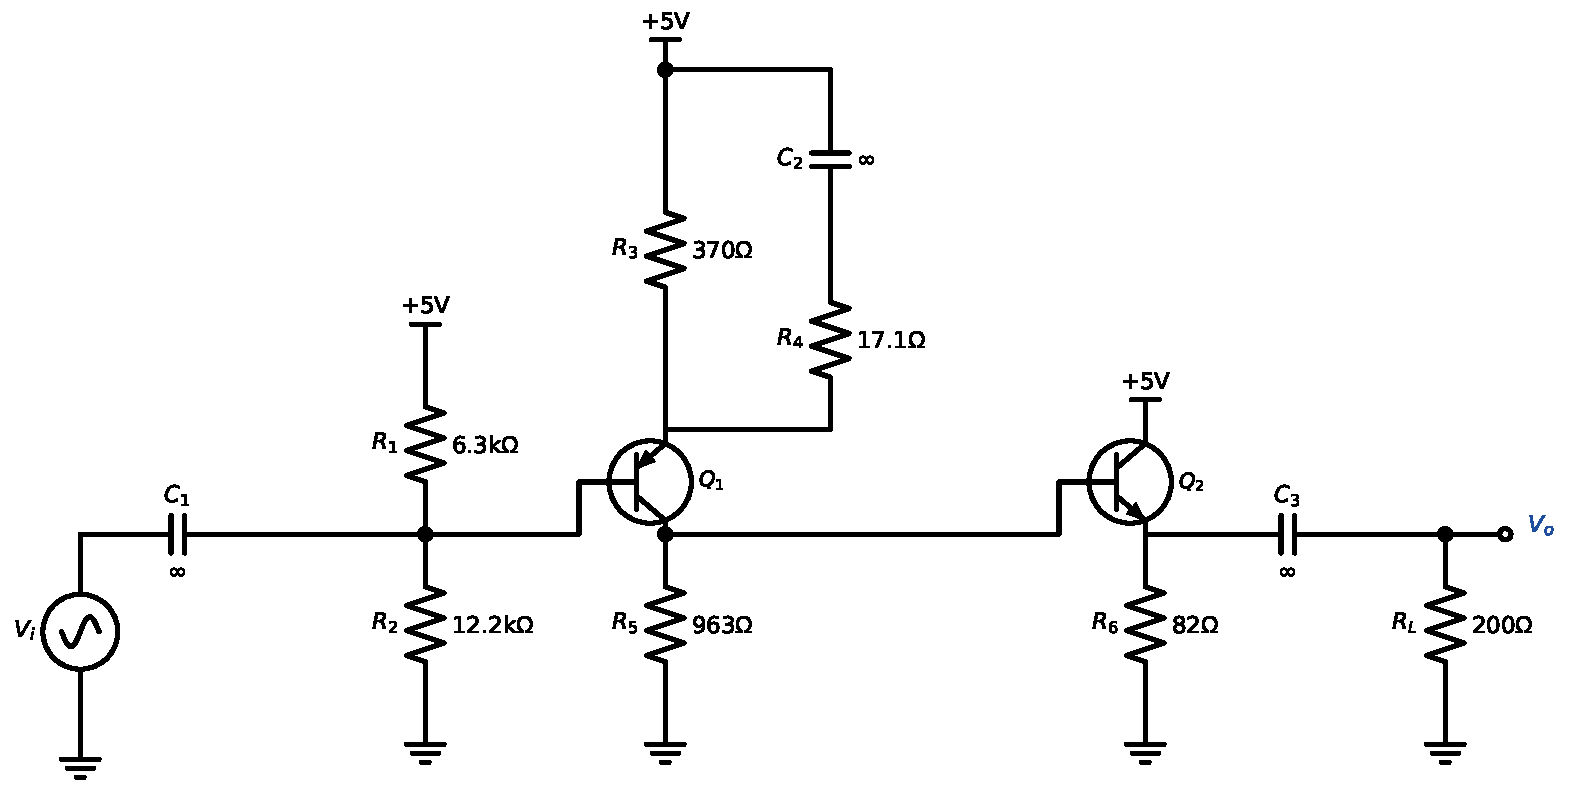
\includegraphics[width=0.9\linewidth,height=6.5cm,keepaspectratio]{p09_designed}\end{center}

\begin{ansbox}
$R_{1} = 6.3\,\mathrm{k}\Omega$,\quad $R_{2} = 12.2\,\mathrm{k}\Omega$,\quad $R_{3} = 370\,\Omega$,\quad $R_{4} = 17.1\,\Omega$,\quad $R_{5} = 963\,\Omega$,\quad $R_{6} = 82\,\Omega$
\end{ansbox}

\newpage
\subsection*{Solution 4E.10 \hfill Medium}
\begin{center}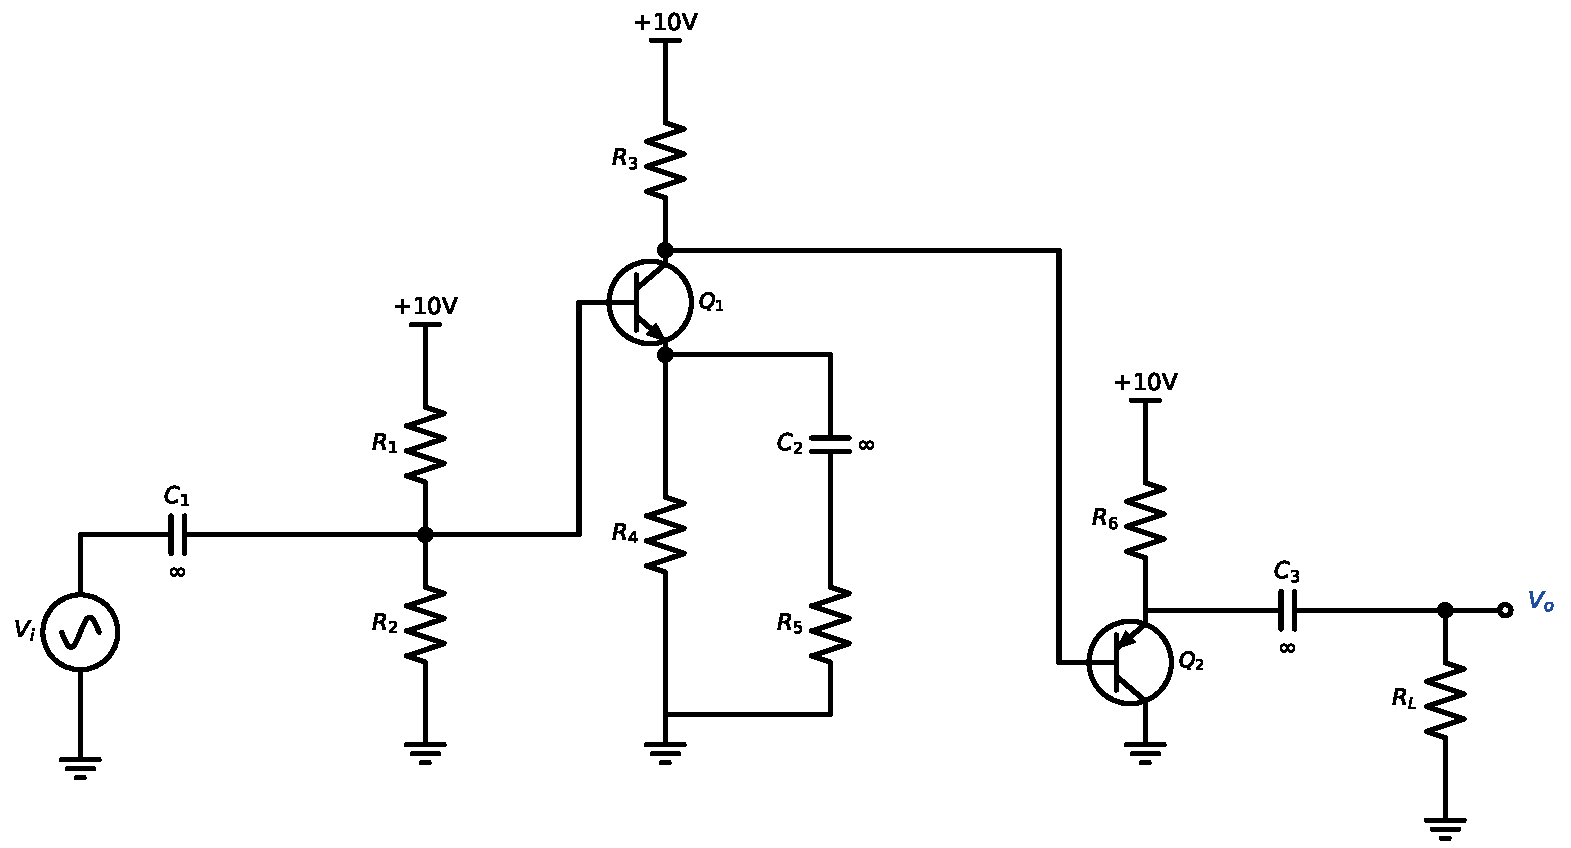
\includegraphics[width=0.9\linewidth,height=6cm,keepaspectratio]{p10_circuit}\end{center}
\solstep{1}{Plan}Name the resistors by their job: $R_{1} = R_{B1}$, $R_{2} = R_{B2}$, $R_{3} = R_{C1}$, $R_{4} = R_{E1}$, $R_{5} = R_{G1}$, $R_{6} = R_H$. Every stage is biased like the one-stage design of the slides: $V_{RE}\ge1$\,V ($V_{BE}$-insensitive), the divider and every collector current much larger than the base current it feeds ($\beta$-insensitive, factor $N$), and $V_{RC}$ as large as the swing allows. Small-signal tools: $r_e = V_T/I_C$, CE gain $|A_v| = \frac{Z_C}{r_e + R_E\|R_G}$, follower gain $\frac{Z_E}{r_e+Z_E}$, base resistance $(\beta+1)(r_e + Z_E)$ (the $\infty$ capacitors put $R_G$ in parallel with $R_E$ for AC only). Design from the output back to the input, because each stage loads the one before it.
\solstep{2}{Output stage and follower}$V_{BE}$-insensitive: $V_{RE1} \ge 1$\,V; use $V_{RE1} = 1$\,V.

To avoid clipping at saturation the collector must be able to swing down by $\hat V_o$ without $V_{CE}$ dropping below $V_{CE,sat}$, and at cutoff $V_{RC}$ must be at least $\hat V_o$: $V_{CC} - \hat V_o - V_{RE1} - V_{CE,sat} \ge V_{RC1} \ge \hat V_o$. Take the largest value (most gain, best linearity): \[V_{RC1} = 10 - 1.8 - 1 - 0.2 = 7\,\mathrm{V} \;\ge\; \hat V_o = 1.8\,\mathrm{V}\ \checkmark\]

Maximum available gain ($R_G=0$, $R_C$ only): $|A_v|_{max} = \frac{R_C}{r_e} = \frac{V_{RC1}/I_C}{V_T/I_C} = \frac{V_{RC1}}{V_T} = \frac{7}{0.025} = 280 \ge 100$ \checkmark

Follower $Q_{2}$: its emitter sits at $0.7$\,V from the collector of $Q_{1}$, so $V_{RH} = V_{RC1} - 0.7 = 6.3\,\mathrm{V}$. To avoid current clipping the DC current in $R_H$ must stay larger than the peak current pushed into $R_L$: \[\frac{V_{RC1} - 0.7 - \hat V_o}{R_H} \ge \frac{\hat V_o}{R_L} \Rightarrow R_H \le R_L\frac{V_{RC1} - 0.7 - \hat V_o}{\hat V_o} = 300\,\Omega\cdot\frac{6.3 - 1.8}{1.8} = 750\,\Omega\]Take the E12 value just below: $R_H = \mathbf{680\,\Omega}$. Then $I_{C2} \approx \frac{V_{RH}}{R_H} = \frac{6.3}{680\,\Omega} = 9.26\,\mathrm{m}\mathrm{A}$, $r_{e2} = \frac{V_T}{I_{C2}} = 2.7\,\Omega$, and with $R_H \| R_L = 208\,\Omega$:\[A_{v2} = \frac{R_H\|R_L}{r_{e2} + R_H\|R_L} = 0.9872,\qquad R_{i2} = (\beta+1)(r_{e2} + R_H\|R_L) = 21.3\,\mathrm{k}\Omega\]
\solstep{3}{Bias current and resistors}Divider: $V_{RB2} = V_{B1} = 1.7\,\mathrm{V}$, $V_{RB1} = V_{CC} - V_{B1} = 8.3\,\mathrm{V}$ ($|V_{RE1}| + 0.7$ on the emitter side). $\beta$-insensitive: the divider current is $N$ times the base current, $I_{RB} = N\frac{I_{C1}}{\beta}$, $N = 10$. Input resistance (all three in parallel, with $(\beta+1)(r_e + R_E\|R_G) \approx \beta\frac{R_{C1}}{|A_{v1}|} = \beta\frac{V_{RC1}}{I_{C1}|A_{v1}|}$):\[R_i \approx \frac{\beta/I_{C1}}{\frac{N}{V_{RB1}} + \frac{N}{V_{RB2}} + \frac{|A_{v1}|}{V_{RC1}}} \ge R_{i,spec} \;\Rightarrow\; I_{C1} \le \frac{\beta/R_{i,spec}}{\frac{10}{8.3} + \frac{10}{1.7} + \frac{101.3}{7}} = 1.55\,\mathrm{m}\mathrm{A}\]Take the E12 value just below: $I_{C1} = 1.5\,\mathrm{m}\mathrm{A}$. 

\[R_{C1} = \frac{V_{RC1}}{I_{C1}} = \frac{7}{1.5\,\mathrm{m}\mathrm{A}} = \mathbf{4.67\,\mathrm{k}\Omega},\quad R_{E1} = \frac{V_{RE1}}{I_{C1}} = \frac{1}{1.5\,\mathrm{m}\mathrm{A}} = \mathbf{667\,\Omega},\quad r_{e1} = \frac{V_T}{I_{C1}} = 16.7\,\Omega\]

Gain $|A_{v1}| = \frac{R_{C1}\|R_{i2}}{r_{e1} + R_{E1}\|R_{G1}} = 101.3$ with $R_{C1}\|R_{i2} = 3.83\,\mathrm{k}\Omega$:\[R_{E1}\|R_{G1} = \frac{R_{C1}\|R_{i2}}{|A_{v1}|} - r_{e1} = 21.1\,\Omega \;\Rightarrow\; R_{G1} = \frac{1}{\frac{1}{21.1\,\Omega} - \frac{1}{667\,\Omega}} = \mathbf{21.8\,\Omega}\]

\[R_{B1} = \frac{V_{RB1}}{N I_{C1}/\beta} = \frac{8.3}{150\,\mu \mathrm{A}} = \mathbf{55.3\,\mathrm{k}\Omega},\qquad R_{B2} = \frac{V_{RB2}}{N I_{C1}/\beta} = \frac{1.7}{150\,\mu \mathrm{A}} = \mathbf{11.3\,\mathrm{k}\Omega}\]

Check: $R_i = R_{B1}\|R_{B2}\|(\beta+1)(r_{e1} + R_{E1}\|R_{G1}) = 55.3\,\mathrm{k}\Omega\|11.3\,\mathrm{k}\Omega\|3.82\,\mathrm{k}\Omega = 2.715\,\mathrm{k}\Omega$ 

$< 3\,\mathrm{k}\Omega$: the estimate above ignored that $R_{C1}$ is loaded by the next stage (and used $\beta$ for $\beta+1$). Take the next lower E12 value, $I_{C1} = 1.2\,\mathrm{m}\mathrm{A}$, and repeat:

\[R_{C1} = \frac{V_{RC1}}{I_{C1}} = \frac{7}{1.2\,\mathrm{m}\mathrm{A}} = \mathbf{5.83\,\mathrm{k}\Omega},\quad R_{E1} = \frac{V_{RE1}}{I_{C1}} = \frac{1}{1.2\,\mathrm{m}\mathrm{A}} = \mathbf{833\,\Omega},\quad r_{e1} = \frac{V_T}{I_{C1}} = 20.8\,\Omega\]

Gain $|A_{v1}| = \frac{R_{C1}\|R_{i2}}{r_{e1} + R_{E1}\|R_{G1}} = 101.3$ with $R_{C1}\|R_{i2} = 4.58\,\mathrm{k}\Omega$:\[R_{E1}\|R_{G1} = \frac{R_{C1}\|R_{i2}}{|A_{v1}|} - r_{e1} = 24.4\,\Omega \;\Rightarrow\; R_{G1} = \frac{1}{\frac{1}{24.4\,\Omega} - \frac{1}{833\,\Omega}} = \mathbf{25.1\,\Omega}\]

\[R_{B1} = \frac{V_{RB1}}{N I_{C1}/\beta} = \frac{8.3}{120\,\mu \mathrm{A}} = \mathbf{69.2\,\mathrm{k}\Omega},\qquad R_{B2} = \frac{V_{RB2}}{N I_{C1}/\beta} = \frac{1.7}{120\,\mu \mathrm{A}} = \mathbf{14.2\,\mathrm{k}\Omega}\]

Check: $R_i = R_{B1}\|R_{B2}\|(\beta+1)(r_{e1} + R_{E1}\|R_{G1}) = 69.2\,\mathrm{k}\Omega\|14.2\,\mathrm{k}\Omega\|4.57\,\mathrm{k}\Omega = 3.289\,\mathrm{k}\Omega$ $\ge 3\,\mathrm{k}\Omega$ \checkmark.
\solstep{4}{Check by analysis}Solve the finished circuit exactly ($\beta=100$, base currents included) for the DC point, then the small-signal gain with the exact $r_e$ values:\begin{center}\renewcommand{\arraystretch}{1.35}
\begin{tabular}{cccc}
\toprule
 & design $I_C$ & exact $I_C$ & exact $|V_{CE}|$ \\
\midrule
$Q_{1}$ & $1.2\,\mathrm{m}\mathrm{A}$ & $1.04\,\mathrm{m}\mathrm{A}$ & $3.463\,\mathrm{V}$ \\
$Q_{2}$ & $9.26\,\mathrm{m}\mathrm{A}$ & $7.22\,\mathrm{m}\mathrm{A}$ & $5.04\,\mathrm{V}$ \\
\bottomrule
\end{tabular}\end{center}
The exact currents are a little off the design values: $N$ only makes each base current $N$ times smaller than the current it disturbs, so the base voltages sag slightly, and along direct-coupled stages each shift is passed on (and amplified) to the next stage. The slides handle this the same way: simulate, then adjust. The exact gain is $|A_v| = 92.3$ instead of $100$ (the hand design ignored $\alpha$ and the base currents). As the slides suggest, trim $R_{G1}$: the gain is proportional to $1/(r_{e1} + R_{E1}\|R_{G1})$, so scale that sum by $92.3/100$ (exact $r_{e1} = 24\,\Omega$):\[R_{E1}\|R_{G1} = (24\,\Omega + 24.4\,\Omega)\frac{92.3}{100} - 24\,\Omega = 20.6\,\Omega \;\Rightarrow\; R_{G1} = \mathbf{21.2\,\Omega}\]Re-analysis: $|A_v| = 100$ \checkmark. \begin{itemize}[leftmargin=*,itemsep=2pt]
\item Input resistance (exact): $R_i = 3.26\,\mathrm{k}\Omega$ $\ge 3\,\mathrm{k}\Omega$ \checkmark
\item Output swing: follower current clipping at $\hat V_o = I_{E2}(R_H\|R_L) = 1.503\,\mathrm{V}$; $Q_{1}$ clips (saturation or cutoff) at $\hat V_o = 3.209\,\mathrm{V}$. The smallest, $1.503\,\mathrm{V}$, is $\ge 1.5$\,V \checkmark
\item Distortion: each CE stage adds $HD_2 \approx \frac{\hat v_b}{4V_T}\left(\frac{r_e}{r_e + R_E\|R_G}\right)^2$ ($\hat v_b$ = its input amplitude at the specified output; for one stage this is the slides' $\frac{\hat V_o V_T |A_v|}{4V_{RC}^2}$): THD $\approx 3.7\,\%$ $\le 5\,\%$ \checkmark
\item $V_{BE}$-insensitive: $V_{RE1} = 1$\,V $\ge 1$\,V \checkmark
\end{itemize}

\begin{center}\renewcommand{\arraystretch}{1.35}
\begin{tabular}{ll}
\toprule
resistor & value \\
\midrule
$R_{1}$ ($R_{B1}$) & $69.2\,\mathrm{k}\Omega$ \\
$R_{2}$ ($R_{B2}$) & $14.2\,\mathrm{k}\Omega$ \\
$R_{3}$ ($R_{C1}$) & $5.83\,\mathrm{k}\Omega$ \\
$R_{4}$ ($R_{E1}$) & $833\,\Omega$ \\
$R_{5}$ ($R_{G1}$) & $21.2\,\Omega$ \\
$R_{6}$ ($R_H$) & $680\,\Omega$ \\
\bottomrule
\end{tabular}\end{center}
\begin{center}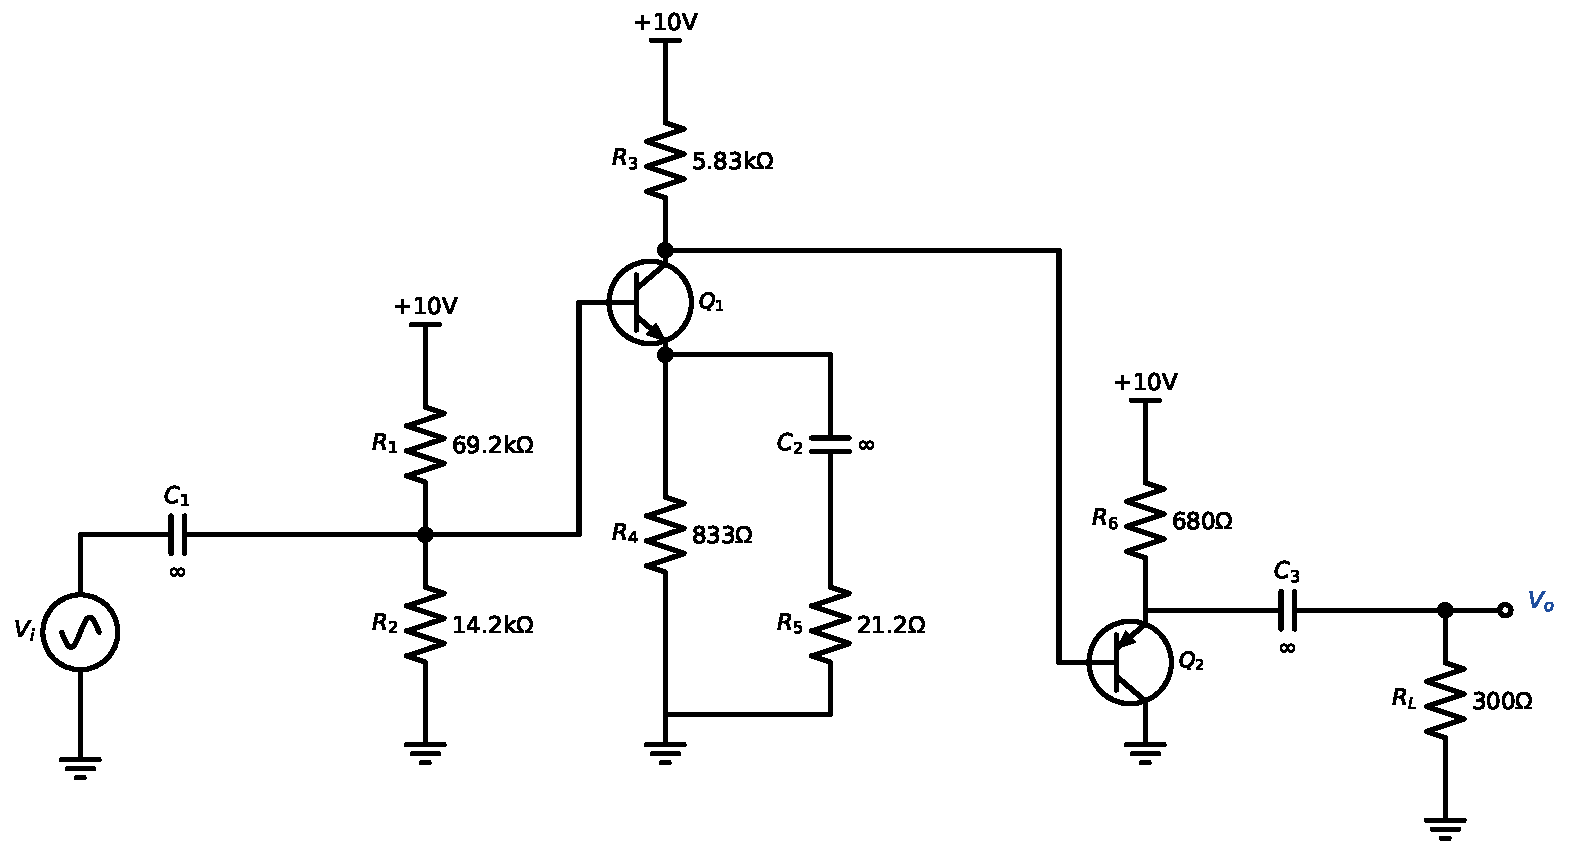
\includegraphics[width=0.9\linewidth,height=6.5cm,keepaspectratio]{p10_designed}\end{center}

\begin{ansbox}
$R_{1} = 69.2\,\mathrm{k}\Omega$,\quad $R_{2} = 14.2\,\mathrm{k}\Omega$,\quad $R_{3} = 5.83\,\mathrm{k}\Omega$,\quad $R_{4} = 833\,\Omega$,\quad $R_{5} = 21.2\,\Omega$,\quad $R_{6} = 680\,\Omega$
\end{ansbox}

\newpage
\subsection*{Solution 4E.11 \hfill Medium}
\begin{center}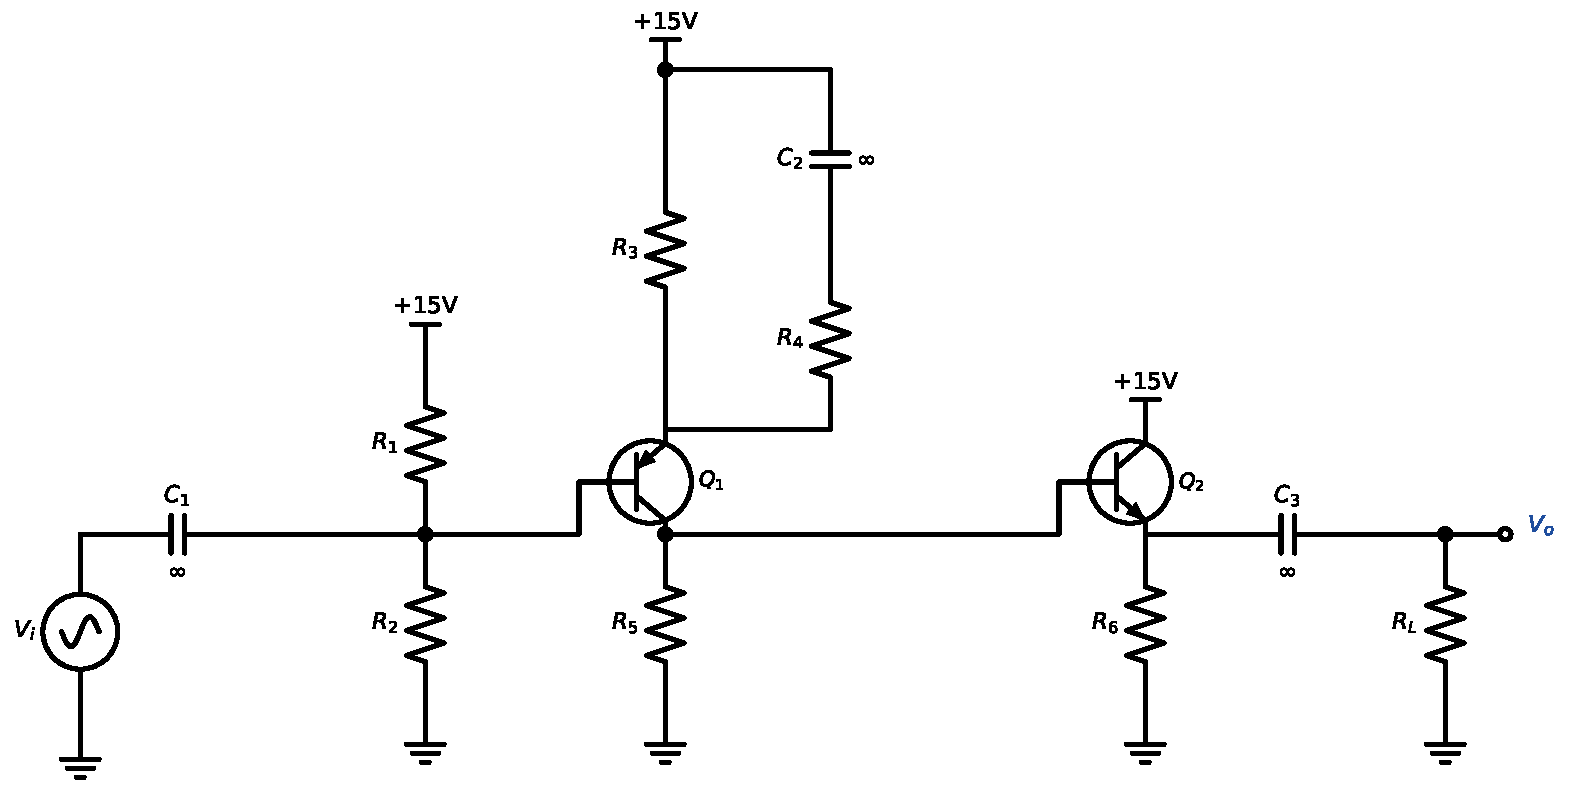
\includegraphics[width=0.9\linewidth,height=6cm,keepaspectratio]{p11_circuit}\end{center}
\solstep{1}{Plan}Name the resistors by their job: $R_{1} = R_{B1}$, $R_{2} = R_{B2}$, $R_{3} = R_{E1}$, $R_{4} = R_{G1}$, $R_{5} = R_{C1}$, $R_{6} = R_H$. Every stage is biased like the one-stage design of the slides: $V_{RE}\ge1$\,V ($V_{BE}$-insensitive), the divider and every collector current much larger than the base current it feeds ($\beta$-insensitive, factor $N$), and $V_{RC}$ as large as the swing allows. Small-signal tools: $r_e = V_T/I_C$, CE gain $|A_v| = \frac{Z_C}{r_e + R_E\|R_G}$, follower gain $\frac{Z_E}{r_e+Z_E}$, base resistance $(\beta+1)(r_e + Z_E)$ (the $\infty$ capacitors put $R_G$ in parallel with $R_E$ for AC only). Design from the output back to the input, because each stage loads the one before it.
\solstep{2}{Output stage and follower}$V_{BE}$-insensitive: $V_{RE1} \ge 1$\,V; use $V_{RE1} = 1$\,V.

To avoid clipping at saturation the collector must be able to swing down by $\hat V_o$ without $V_{CE}$ dropping below $V_{CE,sat}$, and at cutoff $V_{RC}$ must be at least $\hat V_o$: $V_{CC} - \hat V_o - V_{RE1} - V_{CE,sat} \ge V_{RC1} \ge \hat V_o$. Take the largest value (most gain, best linearity): \[V_{RC1} = 15 - 3.5 - 1 - 0.2 = 10.3\,\mathrm{V} \;\ge\; \hat V_o = 3.5\,\mathrm{V}\ \checkmark\]

Maximum available gain ($R_G=0$, $R_C$ only): $|A_v|_{max} = \frac{R_C}{r_e} = \frac{V_{RC1}/I_C}{V_T/I_C} = \frac{V_{RC1}}{V_T} = \frac{10.3}{0.025} = 412 \ge 30$ \checkmark

Follower $Q_{2}$: its emitter sits at $0.7$\,V from the collector of $Q_{1}$, so $V_{RH} = V_{RC1} - 0.7 = 9.6\,\mathrm{V}$. To avoid current clipping the DC current in $R_H$ must stay larger than the peak current pushed into $R_L$: \[\frac{V_{RC1} - 0.7 - \hat V_o}{R_H} \ge \frac{\hat V_o}{R_L} \Rightarrow R_H \le R_L\frac{V_{RC1} - 0.7 - \hat V_o}{\hat V_o} = 1\,\mathrm{k}\Omega\cdot\frac{9.6 - 3.5}{3.5} = 1.74\,\mathrm{k}\Omega\]Take the E12 value just below: $R_H = \mathbf{1.5\,\mathrm{k}\Omega}$. Then $I_{C2} \approx \frac{V_{RH}}{R_H} = \frac{9.6}{1.5\,\mathrm{k}\Omega} = 6.4\,\mathrm{m}\mathrm{A}$, $r_{e2} = \frac{V_T}{I_{C2}} = 3.91\,\Omega$, and with $R_H \| R_L = 600\,\Omega$:\[A_{v2} = \frac{R_H\|R_L}{r_{e2} + R_H\|R_L} = 0.9935,\qquad R_{i2} = (\beta+1)(r_{e2} + R_H\|R_L) = 61\,\mathrm{k}\Omega\]
\solstep{3}{Bias current and resistors}Divider: $V_{RB2} = V_{B1} = 13.3\,\mathrm{V}$, $V_{RB1} = V_{CC} - V_{B1} = 1.7\,\mathrm{V}$ ($|V_{RE1}| + 0.7$ on the emitter side). $\beta$-insensitive: the divider current is $N$ times the base current, $I_{RB} = N\frac{I_{C1}}{\beta}$, $N = 20$. Input resistance (all three in parallel, with $(\beta+1)(r_e + R_E\|R_G) \approx \beta\frac{R_{C1}}{|A_{v1}|} = \beta\frac{V_{RC1}}{I_{C1}|A_{v1}|}$):\[R_i \approx \frac{\beta/I_{C1}}{\frac{N}{V_{RB1}} + \frac{N}{V_{RB2}} + \frac{|A_{v1}|}{V_{RC1}}} \ge R_{i,spec} \;\Rightarrow\; I_{C1} \le \frac{\beta/R_{i,spec}}{\frac{20}{1.7} + \frac{20}{13.3} + \frac{30.2}{10.3}} = 617\,\mu \mathrm{A}\]Take the E12 value just below: $I_{C1} = 560\,\mu \mathrm{A}$. 

\[R_{C1} = \frac{V_{RC1}}{I_{C1}} = \frac{10.3}{560\,\mu \mathrm{A}} = \mathbf{18.4\,\mathrm{k}\Omega},\quad R_{E1} = \frac{V_{RE1}}{I_{C1}} = \frac{1}{560\,\mu \mathrm{A}} = \mathbf{1.79\,\mathrm{k}\Omega},\quad r_{e1} = \frac{V_T}{I_{C1}} = 44.6\,\Omega\]

Gain $|A_{v1}| = \frac{R_{C1}\|R_{i2}}{r_{e1} + R_{E1}\|R_{G1}} = 30.2$ with $R_{C1}\|R_{i2} = 14.1\,\mathrm{k}\Omega$:\[R_{E1}\|R_{G1} = \frac{R_{C1}\|R_{i2}}{|A_{v1}|} - r_{e1} = 423\,\Omega \;\Rightarrow\; R_{G1} = \frac{1}{\frac{1}{423\,\Omega} - \frac{1}{1.79\,\mathrm{k}\Omega}} = \mathbf{555\,\Omega}\]

\[R_{B1} = \frac{V_{RB1}}{N I_{C1}/\beta} = \frac{1.7}{112\,\mu \mathrm{A}} = \mathbf{15.2\,\mathrm{k}\Omega},\qquad R_{B2} = \frac{V_{RB2}}{N I_{C1}/\beta} = \frac{13.3}{112\,\mu \mathrm{A}} = \mathbf{119\,\mathrm{k}\Omega}\]

Check: $R_i = R_{B1}\|R_{B2}\|(\beta+1)(r_{e1} + R_{E1}\|R_{G1}) = 15.2\,\mathrm{k}\Omega\|119\,\mathrm{k}\Omega\|47.3\,\mathrm{k}\Omega = 10.48\,\mathrm{k}\Omega$ $\ge 10\,\mathrm{k}\Omega$ \checkmark.
\solstep{4}{Check by analysis}Solve the finished circuit exactly ($\beta=100$, base currents included) for the DC point, then the small-signal gain with the exact $r_e$ values:\begin{center}\renewcommand{\arraystretch}{1.35}
\begin{tabular}{cccc}
\toprule
 & design $I_C$ & exact $I_C$ & exact $|V_{CE}|$ \\
\midrule
$Q_{1}$ & $560\,\mu \mathrm{A}$ & $516\,\mu \mathrm{A}$ & $5.531\,\mathrm{V}$ \\
$Q_{2}$ & $6.4\,\mathrm{m}\mathrm{A}$ & $5.17\,\mathrm{m}\mathrm{A}$ & $7.162\,\mathrm{V}$ \\
\bottomrule
\end{tabular}\end{center}
The exact currents are a little off the design values: $N$ only makes each base current $N$ times smaller than the current it disturbs, so the base voltages sag slightly, and along direct-coupled stages each shift is passed on (and amplified) to the next stage. The slides handle this the same way: simulate, then adjust. The exact gain is $|A_v| = 29.43$ instead of $30$ (the hand design ignored $\alpha$ and the base currents). As the slides suggest, trim $R_{G1}$: the gain is proportional to $1/(r_{e1} + R_{E1}\|R_{G1})$, so scale that sum by $29.43/30$ (exact $r_{e1} = 48.5\,\Omega$):\[R_{E1}\|R_{G1} = (48.5\,\Omega + 423\,\Omega)\frac{29.43}{30} - 48.5\,\Omega = 414\,\Omega \;\Rightarrow\; R_{G1} = \mathbf{540\,\Omega}\]Re-analysis: $|A_v| = 30$ \checkmark. \begin{itemize}[leftmargin=*,itemsep=2pt]
\item Input resistance (exact): $R_i = 10.4\,\mathrm{k}\Omega$ $\ge 10\,\mathrm{k}\Omega$ \checkmark
\item Output swing: follower current clipping at $\hat V_o = I_{E2}(R_H\|R_L) = 3.104\,\mathrm{V}$; $Q_{1}$ clips (saturation or cutoff) at $\hat V_o = 5.289\,\mathrm{V}$. The smallest, $3.104\,\mathrm{V}$, is $\ge 3$\,V \checkmark
\item Distortion: each CE stage adds $HD_2 \approx \frac{\hat v_b}{4V_T}\left(\frac{r_e}{r_e + R_E\|R_G}\right)^2$ ($\hat v_b$ = its input amplitude at the specified output; for one stage this is the slides' $\frac{\hat V_o V_T |A_v|}{4V_{RC}^2}$): THD $\approx 1.1\,\%$ $\le 3\,\%$ \checkmark
\item $V_{BE}$-insensitive: $V_{RE1} = 1$\,V $\ge 1$\,V \checkmark
\end{itemize}

\begin{center}\renewcommand{\arraystretch}{1.35}
\begin{tabular}{ll}
\toprule
resistor & value \\
\midrule
$R_{1}$ ($R_{B1}$) & $15.2\,\mathrm{k}\Omega$ \\
$R_{2}$ ($R_{B2}$) & $119\,\mathrm{k}\Omega$ \\
$R_{3}$ ($R_{E1}$) & $1.79\,\mathrm{k}\Omega$ \\
$R_{4}$ ($R_{G1}$) & $540\,\Omega$ \\
$R_{5}$ ($R_{C1}$) & $18.4\,\mathrm{k}\Omega$ \\
$R_{6}$ ($R_H$) & $1.5\,\mathrm{k}\Omega$ \\
\bottomrule
\end{tabular}\end{center}
\begin{center}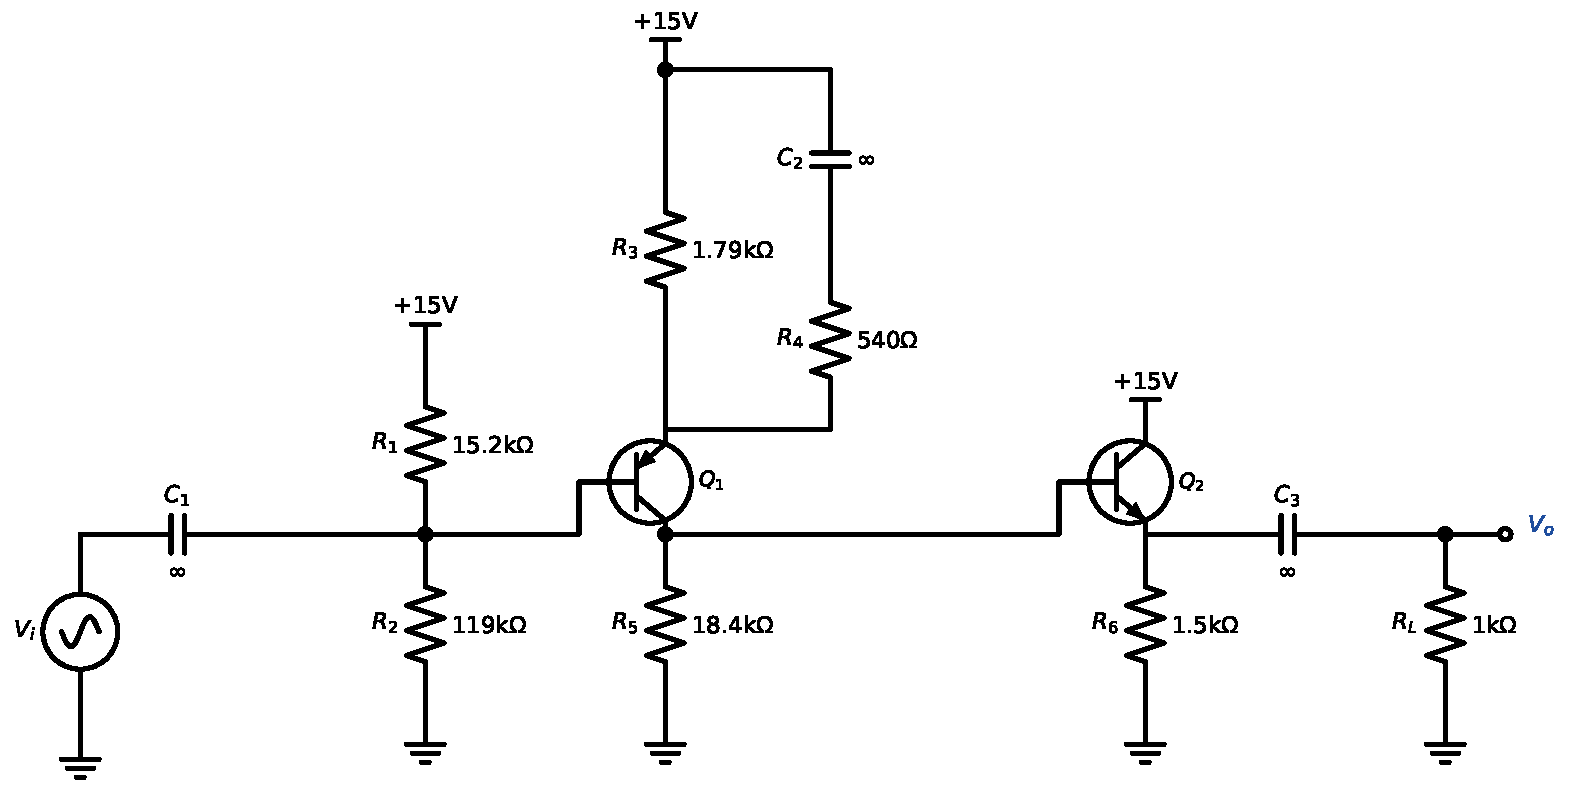
\includegraphics[width=0.9\linewidth,height=6.5cm,keepaspectratio]{p11_designed}\end{center}

\begin{ansbox}
$R_{1} = 15.2\,\mathrm{k}\Omega$,\quad $R_{2} = 119\,\mathrm{k}\Omega$,\quad $R_{3} = 1.79\,\mathrm{k}\Omega$,\quad $R_{4} = 540\,\Omega$,\quad $R_{5} = 18.4\,\mathrm{k}\Omega$,\quad $R_{6} = 1.5\,\mathrm{k}\Omega$
\end{ansbox}

\newpage
\subsection*{Solution 4E.12 \hfill Medium}
\begin{center}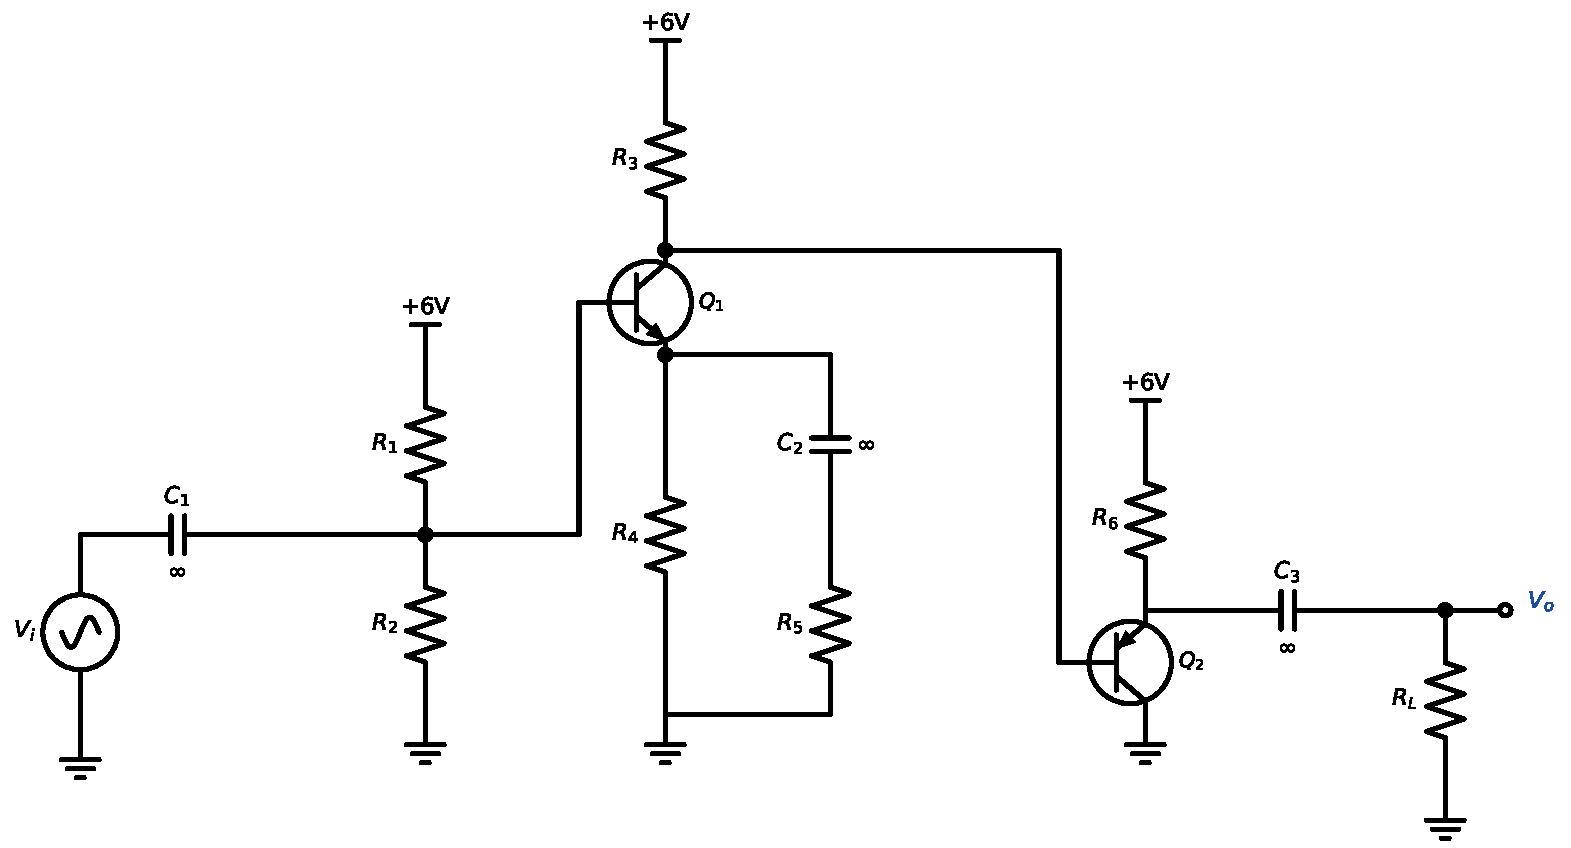
\includegraphics[width=0.9\linewidth,height=6cm,keepaspectratio]{p12_circuit}\end{center}
\solstep{1}{Plan}Name the resistors by their job: $R_{1} = R_{B1}$, $R_{2} = R_{B2}$, $R_{3} = R_{C1}$, $R_{4} = R_{E1}$, $R_{5} = R_{G1}$, $R_{6} = R_H$. Every stage is biased like the one-stage design of the slides: $V_{RE}\ge1$\,V ($V_{BE}$-insensitive), the divider and every collector current much larger than the base current it feeds ($\beta$-insensitive, factor $N$), and $V_{RC}$ as large as the swing allows. Small-signal tools: $r_e = V_T/I_C$, CE gain $|A_v| = \frac{Z_C}{r_e + R_E\|R_G}$, follower gain $\frac{Z_E}{r_e+Z_E}$, base resistance $(\beta+1)(r_e + Z_E)$ (the $\infty$ capacitors put $R_G$ in parallel with $R_E$ for AC only). Design from the output back to the input, because each stage loads the one before it.
\solstep{2}{Output stage and follower}$V_{BE}$-insensitive: $V_{RE1} \ge 1$\,V; use $V_{RE1} = 1$\,V.

To avoid clipping at saturation the collector must be able to swing down by $\hat V_o$ without $V_{CE}$ dropping below $V_{CE,sat}$, and at cutoff $V_{RC}$ must be at least $\hat V_o$: $V_{CC} - \hat V_o - V_{RE1} - V_{CE,sat} \ge V_{RC1} \ge \hat V_o$. Take the largest value (most gain, best linearity): \[V_{RC1} = 6 - 1.2 - 1 - 0.2 = 3.6\,\mathrm{V} \;\ge\; \hat V_o = 1.2\,\mathrm{V}\ \checkmark\]

Maximum available gain ($R_G=0$, $R_C$ only): $|A_v|_{max} = \frac{R_C}{r_e} = \frac{V_{RC1}/I_C}{V_T/I_C} = \frac{V_{RC1}}{V_T} = \frac{3.6}{0.025} = 144 \ge 25$ \checkmark

Follower $Q_{2}$: its emitter sits at $0.7$\,V from the collector of $Q_{1}$, so $V_{RH} = V_{RC1} - 0.7 = 2.9\,\mathrm{V}$. To avoid current clipping the DC current in $R_H$ must stay larger than the peak current pushed into $R_L$: \[\frac{V_{RC1} - 0.7 - \hat V_o}{R_H} \ge \frac{\hat V_o}{R_L} \Rightarrow R_H \le R_L\frac{V_{RC1} - 0.7 - \hat V_o}{\hat V_o} = 100\,\Omega\cdot\frac{2.9 - 1.2}{1.2} = 142\,\Omega\]Take the E12 value just below: $R_H = \mathbf{120\,\Omega}$. Then $I_{C2} \approx \frac{V_{RH}}{R_H} = \frac{2.9}{120\,\Omega} = 24.2\,\mathrm{m}\mathrm{A}$, $r_{e2} = \frac{V_T}{I_{C2}} = 1.03\,\Omega$, and with $R_H \| R_L = 54.5\,\Omega$:\[A_{v2} = \frac{R_H\|R_L}{r_{e2} + R_H\|R_L} = 0.9814,\qquad R_{i2} = (\beta+1)(r_{e2} + R_H\|R_L) = 5.61\,\mathrm{k}\Omega\]
\solstep{3}{Bias current and resistors}Divider: $V_{RB2} = V_{B1} = 1.7\,\mathrm{V}$, $V_{RB1} = V_{CC} - V_{B1} = 4.3\,\mathrm{V}$ ($|V_{RE1}| + 0.7$ on the emitter side). $\beta$-insensitive: the divider current is $N$ times the base current, $I_{RB} = N\frac{I_{C1}}{\beta}$, $N = 10$. Input resistance (all three in parallel, with $(\beta+1)(r_e + R_E\|R_G) \approx \beta\frac{R_{C1}}{|A_{v1}|} = \beta\frac{V_{RC1}}{I_{C1}|A_{v1}|}$):\[R_i \approx \frac{\beta/I_{C1}}{\frac{N}{V_{RB1}} + \frac{N}{V_{RB2}} + \frac{|A_{v1}|}{V_{RC1}}} \ge R_{i,spec} \;\Rightarrow\; I_{C1} \le \frac{\beta/R_{i,spec}}{\frac{10}{4.3} + \frac{10}{1.7} + \frac{25.47}{3.6}} = 3.27\,\mathrm{m}\mathrm{A}\]Take the E12 value just below: $I_{C1} = 2.7\,\mathrm{m}\mathrm{A}$. 

\[R_{C1} = \frac{V_{RC1}}{I_{C1}} = \frac{3.6}{2.7\,\mathrm{m}\mathrm{A}} = \mathbf{1.33\,\mathrm{k}\Omega},\quad R_{E1} = \frac{V_{RE1}}{I_{C1}} = \frac{1}{2.7\,\mathrm{m}\mathrm{A}} = \mathbf{370\,\Omega},\quad r_{e1} = \frac{V_T}{I_{C1}} = 9.26\,\Omega\]

Gain $|A_{v1}| = \frac{R_{C1}\|R_{i2}}{r_{e1} + R_{E1}\|R_{G1}} = 25.47$ with $R_{C1}\|R_{i2} = 1.08\,\mathrm{k}\Omega$:\[R_{E1}\|R_{G1} = \frac{R_{C1}\|R_{i2}}{|A_{v1}|} - r_{e1} = 33\,\Omega \;\Rightarrow\; R_{G1} = \frac{1}{\frac{1}{33\,\Omega} - \frac{1}{370\,\Omega}} = \mathbf{36.3\,\Omega}\]

\[R_{B1} = \frac{V_{RB1}}{N I_{C1}/\beta} = \frac{4.3}{270\,\mu \mathrm{A}} = \mathbf{15.9\,\mathrm{k}\Omega},\qquad R_{B2} = \frac{V_{RB2}}{N I_{C1}/\beta} = \frac{1.7}{270\,\mu \mathrm{A}} = \mathbf{6.3\,\mathrm{k}\Omega}\]

Check: $R_i = R_{B1}\|R_{B2}\|(\beta+1)(r_{e1} + R_{E1}\|R_{G1}) = 15.9\,\mathrm{k}\Omega\|6.3\,\mathrm{k}\Omega\|4.27\,\mathrm{k}\Omega = 2.194\,\mathrm{k}\Omega$ $\ge 2\,\mathrm{k}\Omega$ \checkmark.
\solstep{4}{Check by analysis}Solve the finished circuit exactly ($\beta=100$, base currents included) for the DC point, then the small-signal gain with the exact $r_e$ values:\begin{center}\renewcommand{\arraystretch}{1.35}
\begin{tabular}{cccc}
\toprule
 & design $I_C$ & exact $I_C$ & exact $|V_{CE}|$ \\
\midrule
$Q_{1}$ & $2.7\,\mathrm{m}\mathrm{A}$ & $2.39\,\mathrm{m}\mathrm{A}$ & $2.173\,\mathrm{V}$ \\
$Q_{2}$ & $24.2\,\mathrm{m}\mathrm{A}$ & $18.4\,\mathrm{m}\mathrm{A}$ & $3.765\,\mathrm{V}$ \\
\bottomrule
\end{tabular}\end{center}
The exact currents are a little off the design values: $N$ only makes each base current $N$ times smaller than the current it disturbs, so the base voltages sag slightly, and along direct-coupled stages each shift is passed on (and amplified) to the next stage. The slides handle this the same way: simulate, then adjust. The exact gain is $|A_v| = 23.95$ instead of $25$ (the hand design ignored $\alpha$ and the base currents). As the slides suggest, trim $R_{G1}$: the gain is proportional to $1/(r_{e1} + R_{E1}\|R_{G1})$, so scale that sum by $23.95/25$ (exact $r_{e1} = 10.5\,\Omega$):\[R_{E1}\|R_{G1} = (10.5\,\Omega + 33\,\Omega)\frac{23.95}{25} - 10.5\,\Omega = 31.2\,\Omega \;\Rightarrow\; R_{G1} = \mathbf{34.1\,\Omega}\]Re-analysis: $|A_v| = 25$ \checkmark. \begin{itemize}[leftmargin=*,itemsep=2pt]
\item Input resistance (exact): $R_i = 2.18\,\mathrm{k}\Omega$ $\ge 2\,\mathrm{k}\Omega$ \checkmark
\item Output swing: follower current clipping at $\hat V_o = I_{E2}(R_H\|R_L) = 1.006\,\mathrm{V}$; $Q_{1}$ clips (saturation or cutoff) at $\hat V_o = 1.925\,\mathrm{V}$. The smallest, $1.006\,\mathrm{V}$, is $\ge 1$\,V \checkmark
\item Distortion: each CE stage adds $HD_2 \approx \frac{\hat v_b}{4V_T}\left(\frac{r_e}{r_e + R_E\|R_G}\right)^2$ ($\hat v_b$ = its input amplitude at the specified output; for one stage this is the slides' $\frac{\hat V_o V_T |A_v|}{4V_{RC}^2}$): THD $\approx 2.3\,\%$ $\le 3\,\%$ \checkmark
\item $V_{BE}$-insensitive: $V_{RE1} = 1$\,V $\ge 1$\,V \checkmark
\end{itemize}

\begin{center}\renewcommand{\arraystretch}{1.35}
\begin{tabular}{ll}
\toprule
resistor & value \\
\midrule
$R_{1}$ ($R_{B1}$) & $15.9\,\mathrm{k}\Omega$ \\
$R_{2}$ ($R_{B2}$) & $6.3\,\mathrm{k}\Omega$ \\
$R_{3}$ ($R_{C1}$) & $1.33\,\mathrm{k}\Omega$ \\
$R_{4}$ ($R_{E1}$) & $370\,\Omega$ \\
$R_{5}$ ($R_{G1}$) & $34.1\,\Omega$ \\
$R_{6}$ ($R_H$) & $120\,\Omega$ \\
\bottomrule
\end{tabular}\end{center}
\begin{center}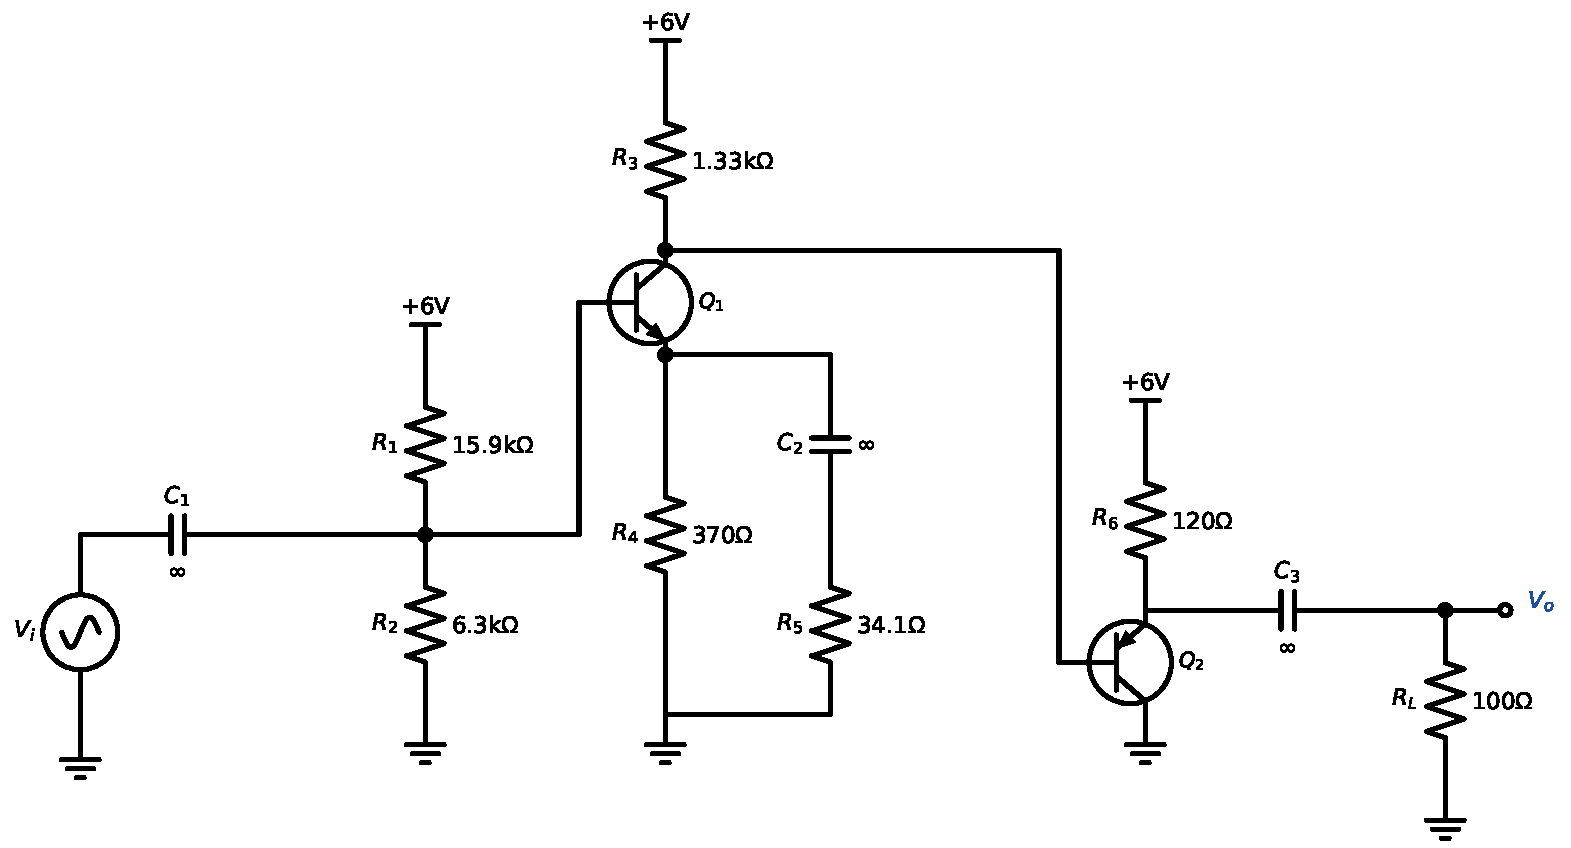
\includegraphics[width=0.9\linewidth,height=6.5cm,keepaspectratio]{p12_designed}\end{center}

\begin{ansbox}
$R_{1} = 15.9\,\mathrm{k}\Omega$,\quad $R_{2} = 6.3\,\mathrm{k}\Omega$,\quad $R_{3} = 1.33\,\mathrm{k}\Omega$,\quad $R_{4} = 370\,\Omega$,\quad $R_{5} = 34.1\,\Omega$,\quad $R_{6} = 120\,\Omega$
\end{ansbox}

\newpage
\subsection*{Solution 4E.13 \hfill Hard}
\begin{center}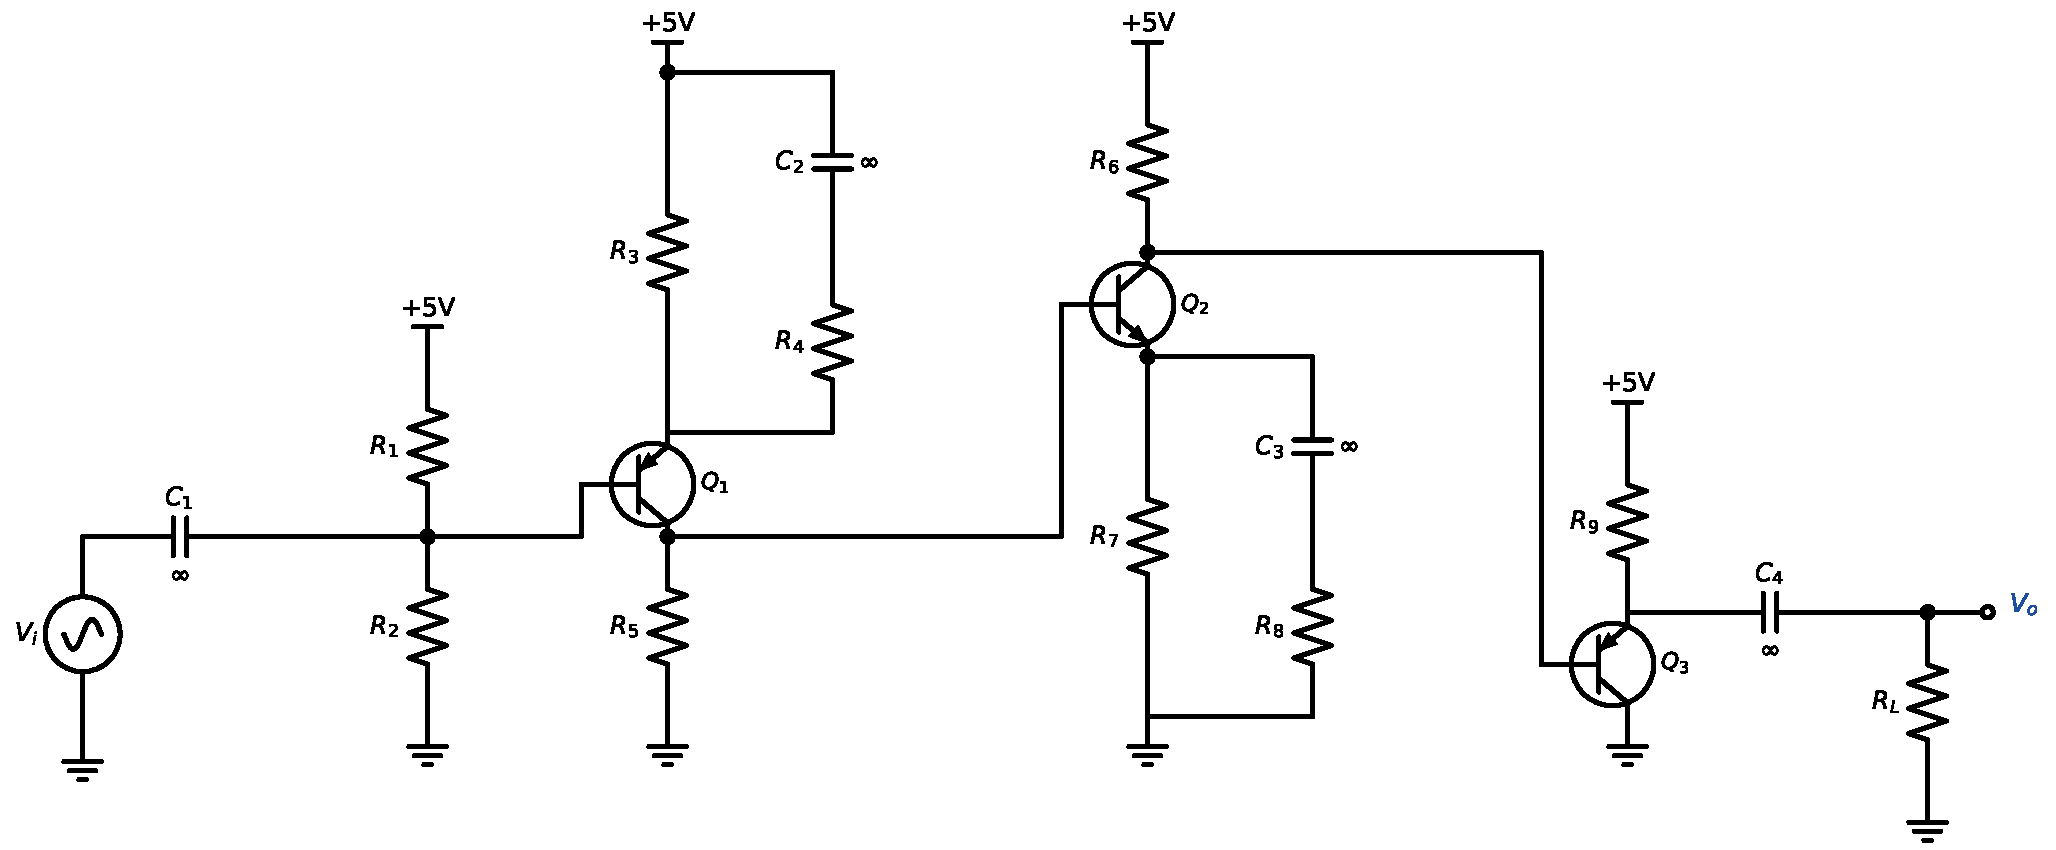
\includegraphics[width=0.9\linewidth,height=6cm,keepaspectratio]{p13_circuit}\end{center}
\solstep{1}{Plan}Name the resistors by their job: $R_{1} = R_{B1}$, $R_{2} = R_{B2}$, $R_{3} = R_{E1}$, $R_{4} = R_{G1}$, $R_{5} = R_{C1}$, $R_{6} = R_{C2}$, $R_{7} = R_{E2}$, $R_{8} = R_{G2}$, $R_{9} = R_H$. Every stage is biased like the one-stage design of the slides: $V_{RE}\ge1$\,V ($V_{BE}$-insensitive), the divider and every collector current much larger than the base current it feeds ($\beta$-insensitive, factor $N$), and $V_{RC}$ as large as the swing allows. Small-signal tools: $r_e = V_T/I_C$, CE gain $|A_v| = \frac{Z_C}{r_e + R_E\|R_G}$, follower gain $\frac{Z_E}{r_e+Z_E}$, base resistance $(\beta+1)(r_e + Z_E)$ (the $\infty$ capacitors put $R_G$ in parallel with $R_E$ for AC only). Design from the output back to the input, because each stage loads the one before it.
\solstep{2}{Output stage and follower}$V_{BE}$-insensitive: $V_{RE2} \ge 1$\,V; use $V_{RE2} = 1$\,V.

Collector swing of $Q_{2}$: about $\hat V_o$ (the follower has a gain close to 1). Largest $V_{RC2}$ without clipping: \[V_{RC2} = V_{CC} - \hat V_o - V_{RE2} - V_{CE,sat} = 5 - 1.3 - 1 - 0.2 = 2.5\,\mathrm{V}\]

Follower $Q_{3}$: its emitter sits at $0.7$\,V from the collector of $Q_{2}$, so $V_{RH} = V_{RC2} - 0.7 = 1.8\,\mathrm{V}$. To avoid current clipping the DC current in $R_H$ must stay larger than the peak current pushed into $R_L$: \[\frac{V_{RC2} - 0.7 - \hat V_o}{R_H} \ge \frac{\hat V_o}{R_L} \Rightarrow R_H \le R_L\frac{V_{RC2} - 0.7 - \hat V_o}{\hat V_o} = 150\,\Omega\cdot\frac{1.8 - 1.3}{1.3} = 57.7\,\Omega\]Use $R_H = \mathbf{50\,\Omega}$ (given). Then $I_{C3} \approx \frac{V_{RH}}{R_H} = \frac{1.8}{50\,\Omega} = 36\,\mathrm{m}\mathrm{A}$, $r_{e3} = \frac{V_T}{I_{C3}} = 694\,\mathrm{m}\Omega$, and with $R_H \| R_L = 37.5\,\Omega$:\[A_{v3} = \frac{R_H\|R_L}{r_{e3} + R_H\|R_L} = 0.9818,\qquad R_{i3} = (\beta+1)(r_{e3} + R_H\|R_L) = 3.86\,\mathrm{k}\Omega\]
\solstep{3}{Stage 2 (common emitter, $Q_{2}$)}$\beta$-insensitive: $I_{C2} \ge N\frac{I_{C3}}{\beta} = 20\cdot\frac{36\,\mathrm{m}\mathrm{A}}{100} = 7.2\,\mathrm{m}\mathrm{A}$; use $I_{C2} = 8\,\mathrm{m}\mathrm{A}$ (given).

\[R_{C2} = \frac{V_{RC2}}{I_{C2}} = \frac{2.5}{8\,\mathrm{m}\mathrm{A}} = \mathbf{312\,\Omega},\quad R_{E2} = \frac{V_{RE2}}{I_{C2}} = \frac{1}{8\,\mathrm{m}\mathrm{A}} = \mathbf{125\,\Omega},\quad r_{e2} = \frac{V_T}{I_{C2}} = 3.12\,\Omega\]

Gain $|A_{v2}| = \frac{R_{C2}\|R_{i3}}{r_{e2} + R_{E2}\|R_{G2}} = 6$ with $R_{C2}\|R_{i3} = 289\,\Omega$:\[R_{E2}\|R_{G2} = \frac{R_{C2}\|R_{i3}}{|A_{v2}|} - r_{e2} = 45.1\,\Omega \;\Rightarrow\; R_{G2} = \frac{1}{\frac{1}{45.1\,\Omega} - \frac{1}{125\,\Omega}} = \mathbf{70.4\,\Omega}\]

Its input resistance: $R_{i2} = (\beta+1)(r_{e2} + R_{E2}\|R_{G2}) = 4.87\,\mathrm{k}\Omega$.
\solstep{4}{Input stage ($Q_1$)}Gain left for stage 1: $|A_{v1}| = \frac{|A_v|}{|A_{v2}| A_{v3}} = \frac{100}{5.891} = 16.98$. The base of $Q_2$ fixes the collector of $Q_1$: $V_{RC1} = 1.7\,\mathrm{V}$. Its collector swing is only $\hat V_o/(\text{gain after it}) = 0.2207\,\mathrm{V}$, so $V_{RE1} \le V_{CC} - V_{RC1} - V_{CE,sat} - 0.221 = 2.879\,\mathrm{V}$; with $V_{RE1} \ge 1$\,V use $V_{RE1} = 1.8$\,V.

Divider: $V_{RB2} = V_{B1} = 2.5\,\mathrm{V}$, $V_{RB1} = V_{CC} - V_{B1} = 2.5\,\mathrm{V}$ ($|V_{RE1}| + 0.7$ on the emitter side). $\beta$-insensitive: the divider current is $N$ times the base current, $I_{RB} = N\frac{I_{C1}}{\beta}$, $N = 20$. Input resistance (all three in parallel, with $(\beta+1)(r_e + R_E\|R_G) \approx \beta\frac{R_{C1}}{|A_{v1}|} = \beta\frac{V_{RC1}}{I_{C1}|A_{v1}|}$):\[R_i \approx \frac{\beta/I_{C1}}{\frac{N}{V_{RB1}} + \frac{N}{V_{RB2}} + \frac{|A_{v1}|}{V_{RC1}}} \ge R_{i,spec} \;\Rightarrow\; I_{C1} \le \frac{\beta/R_{i,spec}}{\frac{20}{2.5} + \frac{20}{2.5} + \frac{16.98}{1.7}} = 1.92\,\mathrm{m}\mathrm{A}\]Take the E12 value just below: $I_{C1} = 1.8\,\mathrm{m}\mathrm{A}$. 

Check $I_{C1} \ge N\frac{I_{C2}}{\beta} = 1.6\,\mathrm{m}\mathrm{A}$ \checkmark. 

\[R_{C1} = \frac{V_{RC1}}{I_{C1}} = \frac{1.7}{1.8\,\mathrm{m}\mathrm{A}} = \mathbf{944\,\Omega},\quad R_{E1} = \frac{V_{RE1}}{I_{C1}} = \frac{1.8}{1.8\,\mathrm{m}\mathrm{A}} = \mathbf{1\,\mathrm{k}\Omega},\quad r_{e1} = \frac{V_T}{I_{C1}} = 13.9\,\Omega\]

Gain $|A_{v1}| = \frac{R_{C1}\|R_{i2}}{r_{e1} + R_{E1}\|R_{G1}} = 16.98$ with $R_{C1}\|R_{i2} = 791\,\Omega$:\[R_{E1}\|R_{G1} = \frac{R_{C1}\|R_{i2}}{|A_{v1}|} - r_{e1} = 32.7\,\Omega \;\Rightarrow\; R_{G1} = \frac{1}{\frac{1}{32.7\,\Omega} - \frac{1}{1\,\mathrm{k}\Omega}} = \mathbf{33.8\,\Omega}\]

\[R_{B1} = \frac{V_{RB1}}{N I_{C1}/\beta} = \frac{2.5}{360\,\mu \mathrm{A}} = \mathbf{6.94\,\mathrm{k}\Omega},\qquad R_{B2} = \frac{V_{RB2}}{N I_{C1}/\beta} = \frac{2.5}{360\,\mu \mathrm{A}} = \mathbf{6.94\,\mathrm{k}\Omega}\]

Check: $R_i = R_{B1}\|R_{B2}\|(\beta+1)(r_{e1} + R_{E1}\|R_{G1}) = 6.94\,\mathrm{k}\Omega\|6.94\,\mathrm{k}\Omega\|4.71\,\mathrm{k}\Omega = 1.998\,\mathrm{k}\Omega$ 

$< 2\,\mathrm{k}\Omega$: the estimate above ignored that $R_{C1}$ is loaded by the next stage (and used $\beta$ for $\beta+1$). Take the next lower E12 value, $I_{C1} = 1.5\,\mathrm{m}\mathrm{A}$, and repeat:

\[R_{C1} = \frac{V_{RC1}}{I_{C1}} = \frac{1.7}{1.5\,\mathrm{m}\mathrm{A}} = \mathbf{1.13\,\mathrm{k}\Omega},\quad R_{E1} = \frac{V_{RE1}}{I_{C1}} = \frac{1.8}{1.5\,\mathrm{m}\mathrm{A}} = \mathbf{1.2\,\mathrm{k}\Omega},\quad r_{e1} = \frac{V_T}{I_{C1}} = 16.7\,\Omega\]

Gain $|A_{v1}| = \frac{R_{C1}\|R_{i2}}{r_{e1} + R_{E1}\|R_{G1}} = 16.98$ with $R_{C1}\|R_{i2} = 919\,\Omega$:\[R_{E1}\|R_{G1} = \frac{R_{C1}\|R_{i2}}{|A_{v1}|} - r_{e1} = 37.5\,\Omega \;\Rightarrow\; R_{G1} = \frac{1}{\frac{1}{37.5\,\Omega} - \frac{1}{1.2\,\mathrm{k}\Omega}} = \mathbf{38.7\,\Omega}\]

\[R_{B1} = \frac{V_{RB1}}{N I_{C1}/\beta} = \frac{2.5}{300\,\mu \mathrm{A}} = \mathbf{8.33\,\mathrm{k}\Omega},\qquad R_{B2} = \frac{V_{RB2}}{N I_{C1}/\beta} = \frac{2.5}{300\,\mu \mathrm{A}} = \mathbf{8.33\,\mathrm{k}\Omega}\]

Check: $R_i = R_{B1}\|R_{B2}\|(\beta+1)(r_{e1} + R_{E1}\|R_{G1}) = 8.33\,\mathrm{k}\Omega\|8.33\,\mathrm{k}\Omega\|5.47\,\mathrm{k}\Omega = 2.365\,\mathrm{k}\Omega$ $\ge 2\,\mathrm{k}\Omega$ \checkmark.
\solstep{5}{Check by analysis}Solve the finished circuit exactly ($\beta=100$, base currents included) for the DC point, then the small-signal gain with the exact $r_e$ values:\begin{center}\renewcommand{\arraystretch}{1.35}
\begin{tabular}{cccc}
\toprule
 & design $I_C$ & exact $I_C$ & exact $|V_{CE}|$ \\
\midrule
$Q_{1}$ & $1.5\,\mathrm{m}\mathrm{A}$ & $1.44\,\mathrm{m}\mathrm{A}$ & $1.709\,\mathrm{V}$ \\
$Q_{2}$ & $8\,\mathrm{m}\mathrm{A}$ & $6.74\,\mathrm{m}\mathrm{A}$ & $2.125\,\mathrm{V}$ \\
$Q_{3}$ & $36\,\mathrm{m}\mathrm{A}$ & $26.2\,\mathrm{m}\mathrm{A}$ & $3.676\,\mathrm{V}$ \\
\bottomrule
\end{tabular}\end{center}
The exact currents are a little off the design values: $N$ only makes each base current $N$ times smaller than the current it disturbs, so the base voltages sag slightly, and along direct-coupled stages each shift is passed on (and amplified) to the next stage. The slides handle this the same way: simulate, then adjust. The exact gain is $|A_v| = 95.16$ instead of $100$ (the hand design ignored $\alpha$ and the base currents). As the slides suggest, trim $R_{G1}$: the gain is proportional to $1/(r_{e1} + R_{E1}\|R_{G1})$, so scale that sum by $95.16/100$ (exact $r_{e1} = 17.4\,\Omega$):\[R_{E1}\|R_{G1} = (17.4\,\Omega + 37.5\,\Omega)\frac{95.16}{100} - 17.4\,\Omega = 34.8\,\Omega \;\Rightarrow\; R_{G1} = \mathbf{35.9\,\Omega}\]Re-analysis: $|A_v| = 100$ \checkmark. \par The follower would clip at $\hat V_o = I_{E3}(R_H\|R_L) = 26.2\,\mathrm{m}\mathrm{A}\times37.5\,\Omega = 0.9833\,\mathrm{V} < 1$\,V: its exact current is below the design value because the base currents shift the DC voltages along the direct-coupled chain. Adjust: lower $R_H$ to the next E12 value, $R_H = \mathbf{47\,\Omega}$ (more follower current), and analyse again. The exact gain is $|A_v| = 99.67$, within $0.5\,\%$ of the specification \checkmark. \begin{itemize}[leftmargin=*,itemsep=2pt]
\item Input resistance (exact): $R_i = 2.33\,\mathrm{k}\Omega$ $\ge 2\,\mathrm{k}\Omega$ \checkmark
\item Output swing: follower current clipping at $\hat V_o = I_{E3}(R_H\|R_L) = 1.042\,\mathrm{V}$; $Q_{2}$ clips (saturation or cutoff) at $\hat V_o = 1.885\,\mathrm{V}$; $Q_{1}$ clips (saturation or cutoff) at $\hat V_o = 7.585\,\mathrm{V}$. The smallest, $1.042\,\mathrm{V}$, is $\ge 1$\,V \checkmark
\item Distortion: each CE stage adds $HD_2 \approx \frac{\hat v_b}{4V_T}\left(\frac{r_e}{r_e + R_E\|R_G}\right)^2$ ($\hat v_b$ = its input amplitude at the specified output; for one stage this is the slides' $\frac{\hat V_o V_T |A_v|}{4V_{RC}^2}$): THD $\approx 1 + 0.96\,\% = 2\,\%$ $\le 3\,\%$ \checkmark
\item $V_{BE}$-insensitive: $V_{RE1} = 1.8$\,V, $V_{RE2} = 1$\,V $\ge 1$\,V \checkmark
\end{itemize}

\begin{center}\renewcommand{\arraystretch}{1.35}
\begin{tabular}{ll}
\toprule
resistor & value \\
\midrule
$R_{1}$ ($R_{B1}$) & $8.33\,\mathrm{k}\Omega$ \\
$R_{2}$ ($R_{B2}$) & $8.33\,\mathrm{k}\Omega$ \\
$R_{3}$ ($R_{E1}$) & $1.2\,\mathrm{k}\Omega$ \\
$R_{4}$ ($R_{G1}$) & $35.9\,\Omega$ \\
$R_{5}$ ($R_{C1}$) & $1.13\,\mathrm{k}\Omega$ \\
$R_{6}$ ($R_{C2}$) & $312\,\Omega$ \\
$R_{7}$ ($R_{E2}$) & $125\,\Omega$ \\
$R_{8}$ ($R_{G2}$) & $70.4\,\Omega$ \\
$R_{9}$ ($R_H$) & $47\,\Omega$ \\
\bottomrule
\end{tabular}\end{center}
\begin{center}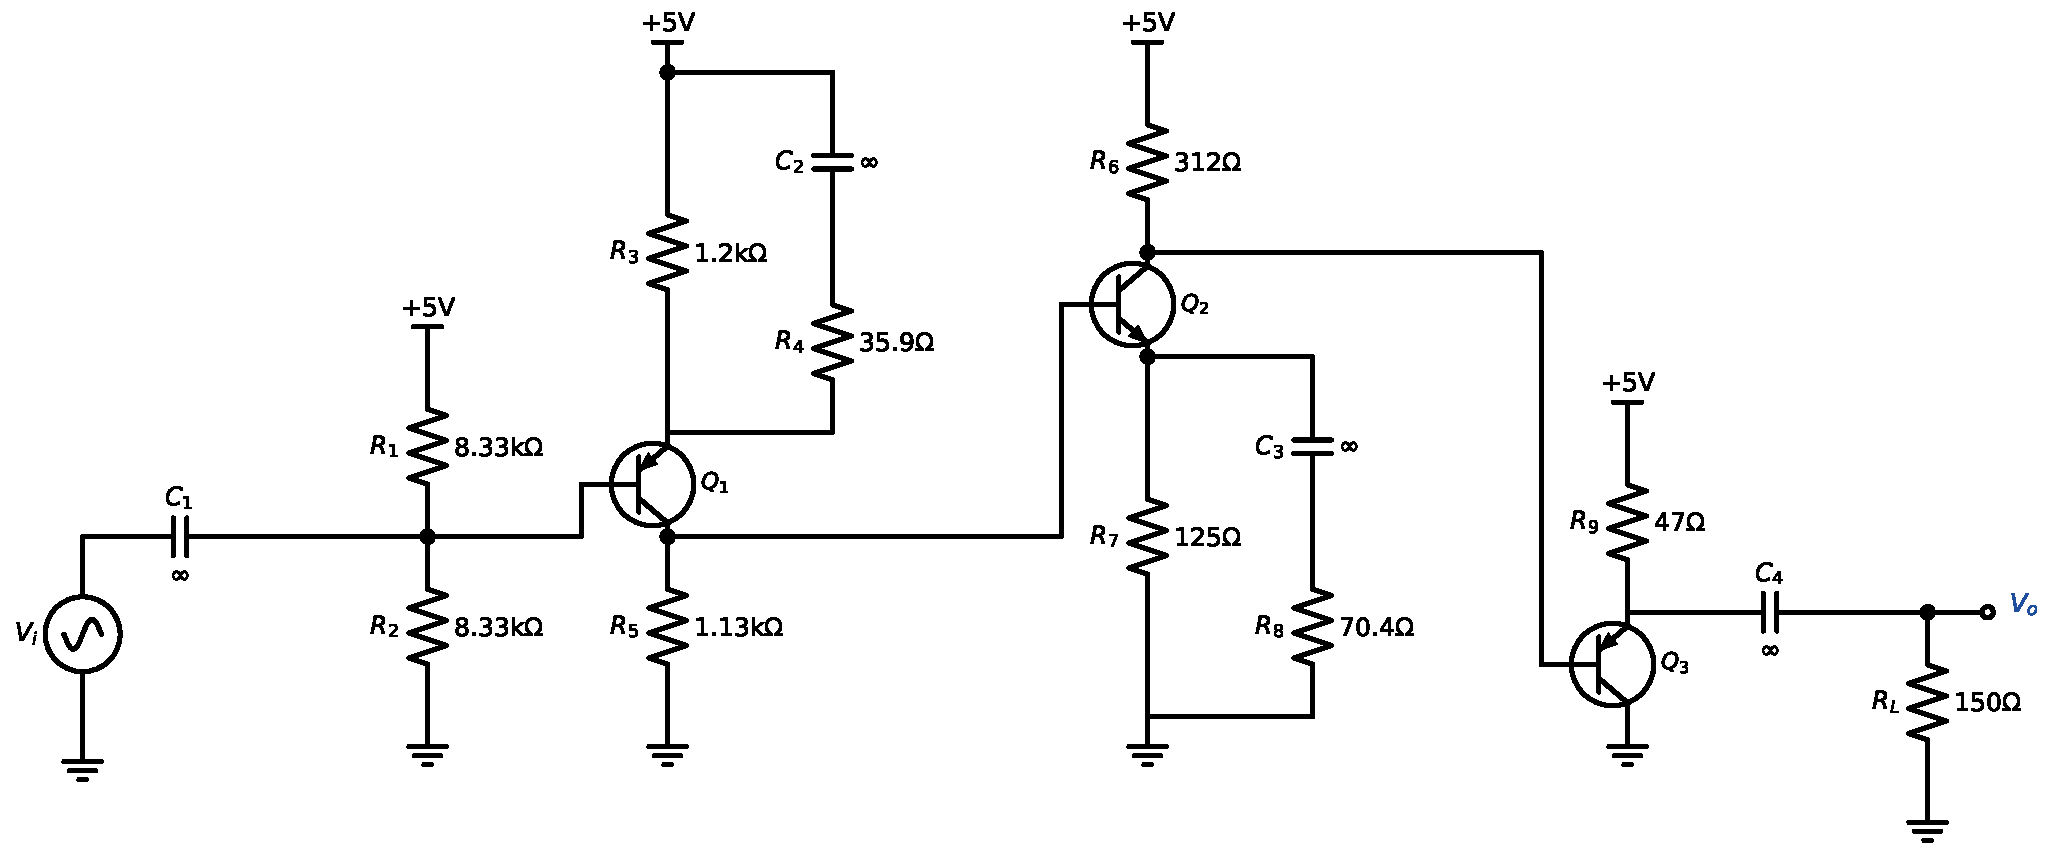
\includegraphics[width=0.9\linewidth,height=6.5cm,keepaspectratio]{p13_designed}\end{center}

\begin{ansbox}
$R_{1} = 8.33\,\mathrm{k}\Omega$,\quad $R_{2} = 8.33\,\mathrm{k}\Omega$,\quad $R_{3} = 1.2\,\mathrm{k}\Omega$,\quad $R_{4} = 35.9\,\Omega$,\quad $R_{5} = 1.13\,\mathrm{k}\Omega$,\quad $R_{6} = 312\,\Omega$,\quad $R_{7} = 125\,\Omega$,\quad $R_{8} = 70.4\,\Omega$,\quad $R_{9} = 47\,\Omega$
\end{ansbox}

\newpage
\subsection*{Solution 4E.14 \hfill Hard}
\begin{center}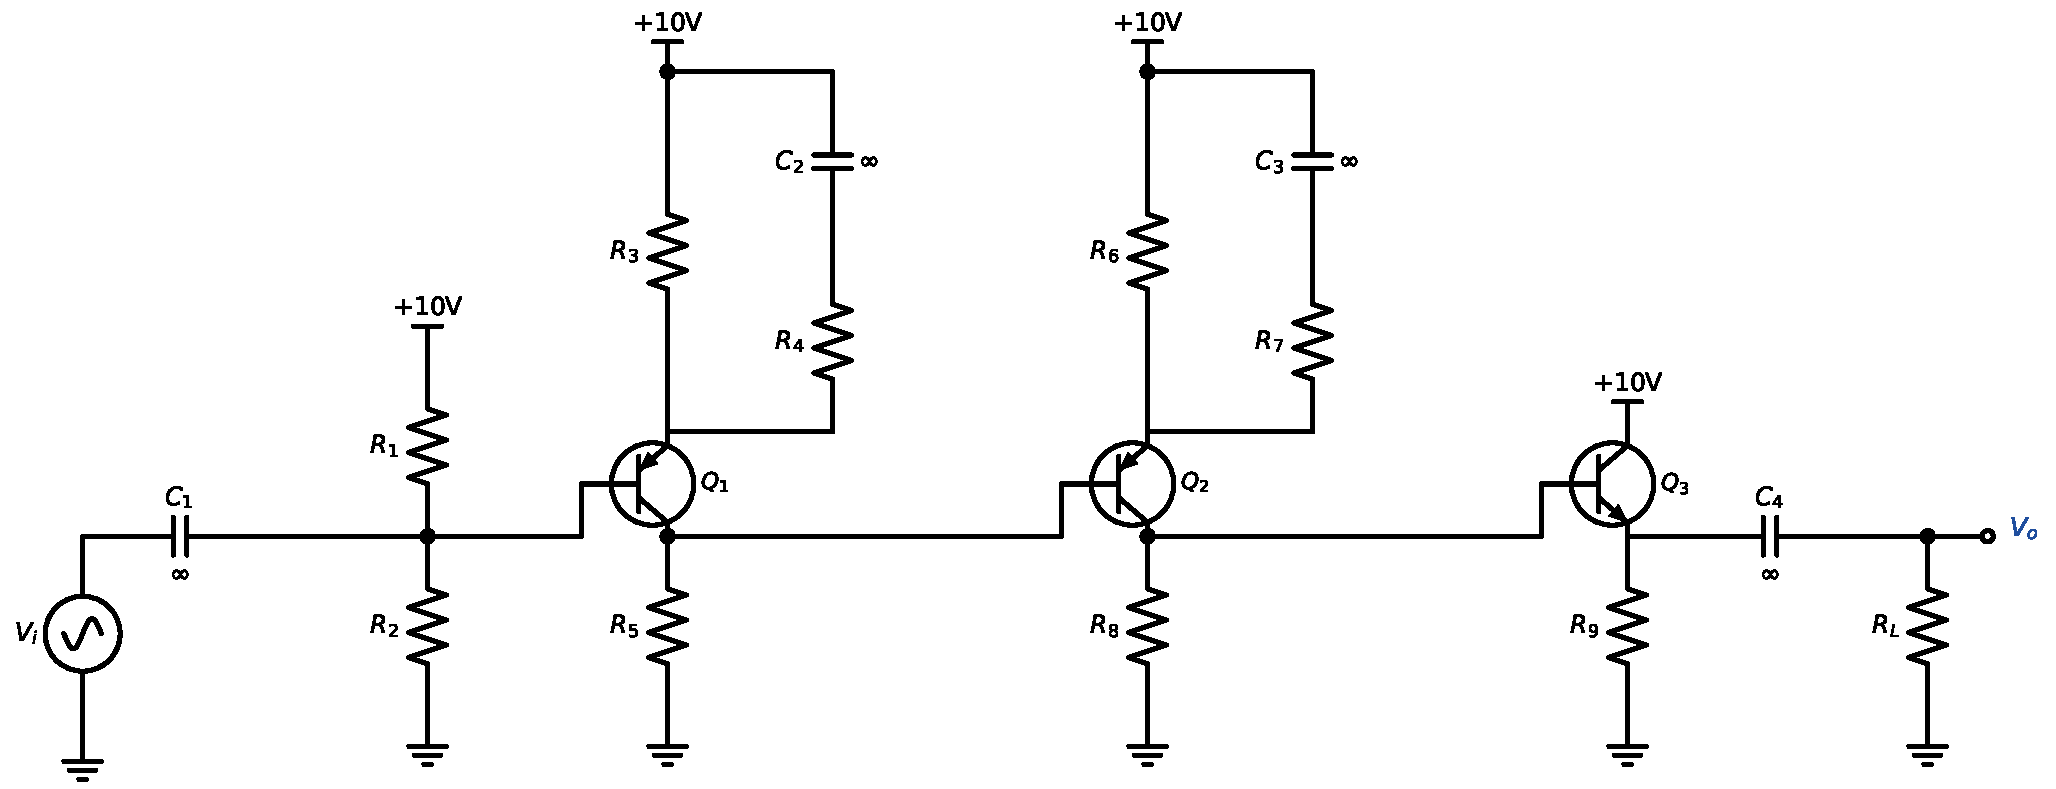
\includegraphics[width=0.9\linewidth,height=6cm,keepaspectratio]{p14_circuit}\end{center}
\solstep{1}{Plan}Name the resistors by their job: $R_{1} = R_{B1}$, $R_{2} = R_{B2}$, $R_{3} = R_{E1}$, $R_{4} = R_{G1}$, $R_{5} = R_{C1}$, $R_{6} = R_{E2}$, $R_{7} = R_{G2}$, $R_{8} = R_{C2}$, $R_{9} = R_H$. Every stage is biased like the one-stage design of the slides: $V_{RE}\ge1$\,V ($V_{BE}$-insensitive), the divider and every collector current much larger than the base current it feeds ($\beta$-insensitive, factor $N$), and $V_{RC}$ as large as the swing allows. Small-signal tools: $r_e = V_T/I_C$, CE gain $|A_v| = \frac{Z_C}{r_e + R_E\|R_G}$, follower gain $\frac{Z_E}{r_e+Z_E}$, base resistance $(\beta+1)(r_e + Z_E)$ (the $\infty$ capacitors put $R_G$ in parallel with $R_E$ for AC only). Design from the output back to the input, because each stage loads the one before it.
\solstep{2}{Output stage and follower}$V_{BE}$-insensitive: $V_{RE2} \ge 1$\,V; use $V_{RE2} = 1$\,V.

Collector swing of $Q_{2}$: about $\hat V_o$ (the follower has a gain close to 1). Largest $V_{RC2}$ without clipping: \[V_{RC2} = V_{CC} - \hat V_o - V_{RE2} - V_{CE,sat} = 10 - 2.4 - 1 - 0.2 = 6.4\,\mathrm{V}\]

Follower $Q_{3}$: its emitter sits at $0.7$\,V from the collector of $Q_{2}$, so $V_{RH} = V_{RC2} - 0.7 = 5.7\,\mathrm{V}$. To avoid current clipping the DC current in $R_H$ must stay larger than the peak current pushed into $R_L$: \[\frac{V_{RC2} - 0.7 - \hat V_o}{R_H} \ge \frac{\hat V_o}{R_L} \Rightarrow R_H \le R_L\frac{V_{RC2} - 0.7 - \hat V_o}{\hat V_o} = 500\,\Omega\cdot\frac{5.7 - 2.4}{2.4} = 687\,\Omega\]Take the E12 value just below: $R_H = \mathbf{680\,\Omega}$. Then $I_{C3} \approx \frac{V_{RH}}{R_H} = \frac{5.7}{680\,\Omega} = 8.38\,\mathrm{m}\mathrm{A}$, $r_{e3} = \frac{V_T}{I_{C3}} = 2.98\,\Omega$, and with $R_H \| R_L = 288\,\Omega$:\[A_{v3} = \frac{R_H\|R_L}{r_{e3} + R_H\|R_L} = 0.9898,\qquad R_{i3} = (\beta+1)(r_{e3} + R_H\|R_L) = 29.4\,\mathrm{k}\Omega\]
\solstep{3}{Stage 2 (common emitter, $Q_{2}$)}$\beta$-insensitive: $I_{C2} \ge N\frac{I_{C3}}{\beta} = 10\cdot\frac{8.38\,\mathrm{m}\mathrm{A}}{100} = 838\,\mu \mathrm{A}$; take the E12 value just above, $I_{C2} = 1\,\mathrm{m}\mathrm{A}$.

\[R_{C2} = \frac{V_{RC2}}{I_{C2}} = \frac{6.4}{1\,\mathrm{m}\mathrm{A}} = \mathbf{6.4\,\mathrm{k}\Omega},\quad R_{E2} = \frac{V_{RE2}}{I_{C2}} = \frac{1}{1\,\mathrm{m}\mathrm{A}} = \mathbf{1\,\mathrm{k}\Omega},\quad r_{e2} = \frac{V_T}{I_{C2}} = 25\,\Omega\]

Gain $|A_{v2}| = \frac{R_{C2}\|R_{i3}}{r_{e2} + R_{E2}\|R_{G2}} = 10$ with $R_{C2}\|R_{i3} = 5.26\,\mathrm{k}\Omega$:\[R_{E2}\|R_{G2} = \frac{R_{C2}\|R_{i3}}{|A_{v2}|} - r_{e2} = 501\,\Omega \;\Rightarrow\; R_{G2} = \frac{1}{\frac{1}{501\,\Omega} - \frac{1}{1\,\mathrm{k}\Omega}} = \mathbf{1\,\mathrm{k}\Omega}\]

Its input resistance: $R_{i2} = (\beta+1)(r_{e2} + R_{E2}\|R_{G2}) = 53.1\,\mathrm{k}\Omega$.
\solstep{4}{Input stage ($Q_1$)}Gain left for stage 1: $|A_{v1}| = \frac{|A_v|}{|A_{v2}| A_{v3}} = \frac{200}{9.898} = 20.21$. The base of $Q_2$ fixes the collector of $Q_1$: $V_{RC1} = 8.3\,\mathrm{V}$. Its collector swing is only $\hat V_o/(\text{gain after it}) = 0.2425\,\mathrm{V}$, so $V_{RE1} \le V_{CC} - V_{RC1} - V_{CE,sat} - 0.242 = 1.258\,\mathrm{V}$; with $V_{RE1} \ge 1$\,V use $V_{RE1} = 1$\,V.

Divider: $V_{RB2} = V_{B1} = 8.3\,\mathrm{V}$, $V_{RB1} = V_{CC} - V_{B1} = 1.7\,\mathrm{V}$ ($|V_{RE1}| + 0.7$ on the emitter side). $\beta$-insensitive: the divider current is $N$ times the base current, $I_{RB} = N\frac{I_{C1}}{\beta}$, $N = 10$. Input resistance (all three in parallel, with $(\beta+1)(r_e + R_E\|R_G) \approx \beta\frac{R_{C1}}{|A_{v1}|} = \beta\frac{V_{RC1}}{I_{C1}|A_{v1}|}$):\[R_i \approx \frac{\beta/I_{C1}}{\frac{N}{V_{RB1}} + \frac{N}{V_{RB2}} + \frac{|A_{v1}|}{V_{RC1}}} \ge R_{i,spec} \;\Rightarrow\; I_{C1} \le \frac{\beta/R_{i,spec}}{\frac{10}{1.7} + \frac{10}{8.3} + \frac{20.21}{8.3}} = 2.1\,\mathrm{m}\mathrm{A}\]Take the E12 value just below: $I_{C1} = 1.8\,\mathrm{m}\mathrm{A}$. 

Check $I_{C1} \ge N\frac{I_{C2}}{\beta} = 100\,\mu \mathrm{A}$ \checkmark. 

\[R_{C1} = \frac{V_{RC1}}{I_{C1}} = \frac{8.3}{1.8\,\mathrm{m}\mathrm{A}} = \mathbf{4.61\,\mathrm{k}\Omega},\quad R_{E1} = \frac{V_{RE1}}{I_{C1}} = \frac{1}{1.8\,\mathrm{m}\mathrm{A}} = \mathbf{556\,\Omega},\quad r_{e1} = \frac{V_T}{I_{C1}} = 13.9\,\Omega\]

Gain $|A_{v1}| = \frac{R_{C1}\|R_{i2}}{r_{e1} + R_{E1}\|R_{G1}} = 20.21$ with $R_{C1}\|R_{i2} = 4.24\,\mathrm{k}\Omega$:\[R_{E1}\|R_{G1} = \frac{R_{C1}\|R_{i2}}{|A_{v1}|} - r_{e1} = 196\,\Omega \;\Rightarrow\; R_{G1} = \frac{1}{\frac{1}{196\,\Omega} - \frac{1}{556\,\Omega}} = \mathbf{303\,\Omega}\]

\[R_{B1} = \frac{V_{RB1}}{N I_{C1}/\beta} = \frac{1.7}{180\,\mu \mathrm{A}} = \mathbf{9.44\,\mathrm{k}\Omega},\qquad R_{B2} = \frac{V_{RB2}}{N I_{C1}/\beta} = \frac{8.3}{180\,\mu \mathrm{A}} = \mathbf{46.1\,\mathrm{k}\Omega}\]

Check: $R_i = R_{B1}\|R_{B2}\|(\beta+1)(r_{e1} + R_{E1}\|R_{G1}) = 9.44\,\mathrm{k}\Omega\|46.1\,\mathrm{k}\Omega\|21.2\,\mathrm{k}\Omega = 5.723\,\mathrm{k}\Omega$ $\ge 5\,\mathrm{k}\Omega$ \checkmark.
\solstep{5}{Check by analysis}Solve the finished circuit exactly ($\beta=100$, base currents included) for the DC point, then the small-signal gain with the exact $r_e$ values:\begin{center}\renewcommand{\arraystretch}{1.35}
\begin{tabular}{cccc}
\toprule
 & design $I_C$ & exact $I_C$ & exact $|V_{CE}|$ \\
\midrule
$Q_{1}$ & $1.8\,\mathrm{m}\mathrm{A}$ & $1.56\,\mathrm{m}\mathrm{A}$ & $1.821\,\mathrm{V}$ \\
$Q_{2}$ & $1\,\mathrm{m}\mathrm{A}$ & $1.98\,\mathrm{m}\mathrm{A}$ & $3.641\,\mathrm{V}$ \\
$Q_{3}$ & $8.38\,\mathrm{m}\mathrm{A}$ & $15.9\,\mathrm{m}\mathrm{A}$ & $0.9426\,\mathrm{V}$ \\
\bottomrule
\end{tabular}\end{center}
The exact currents are a little off the design values: $N$ only makes each base current $N$ times smaller than the current it disturbs, so the base voltages sag slightly, and along direct-coupled stages each shift is passed on (and amplified) to the next stage. The slides handle this the same way: simulate, then adjust. The exact gain is $|A_v| = 199.2$, within $0.5\,\%$ of the specification \checkmark. \begin{itemize}[leftmargin=*,itemsep=2pt]
\item Input resistance (exact): $R_i = 5.74\,\mathrm{k}\Omega$ $\ge 5\,\mathrm{k}\Omega$ \checkmark
\item Output swing: follower current clipping at $\hat V_o = I_{E3}(R_H\|R_L) = 4.591\,\mathrm{V}$; $Q_{2}$ clips (saturation or cutoff) at $\hat V_o = 3.422\,\mathrm{V}$; $Q_{1}$ clips (saturation or cutoff) at $\hat V_o = 16.33\,\mathrm{V}$. The smallest, $3.422\,\mathrm{V}$, is $\ge 2$\,V \checkmark
\item Distortion: each CE stage adds $HD_2 \approx \frac{\hat v_b}{4V_T}\left(\frac{r_e}{r_e + R_E\|R_G}\right)^2$ ($\hat v_b$ = its input amplitude at the specified output; for one stage this is the slides' $\frac{\hat V_o V_T |A_v|}{4V_{RC}^2}$): THD $\approx 0.057 + 0.12\,\% = 0.18\,\%$ $\le 5\,\%$ \checkmark
\item $V_{BE}$-insensitive: $V_{RE1} = 1$\,V, $V_{RE2} = 1$\,V $\ge 1$\,V \checkmark
\end{itemize}

\begin{center}\renewcommand{\arraystretch}{1.35}
\begin{tabular}{ll}
\toprule
resistor & value \\
\midrule
$R_{1}$ ($R_{B1}$) & $9.44\,\mathrm{k}\Omega$ \\
$R_{2}$ ($R_{B2}$) & $46.1\,\mathrm{k}\Omega$ \\
$R_{3}$ ($R_{E1}$) & $556\,\Omega$ \\
$R_{4}$ ($R_{G1}$) & $303\,\Omega$ \\
$R_{5}$ ($R_{C1}$) & $4.61\,\mathrm{k}\Omega$ \\
$R_{6}$ ($R_{E2}$) & $1\,\mathrm{k}\Omega$ \\
$R_{7}$ ($R_{G2}$) & $1\,\mathrm{k}\Omega$ \\
$R_{8}$ ($R_{C2}$) & $6.4\,\mathrm{k}\Omega$ \\
$R_{9}$ ($R_H$) & $680\,\Omega$ \\
\bottomrule
\end{tabular}\end{center}
\begin{center}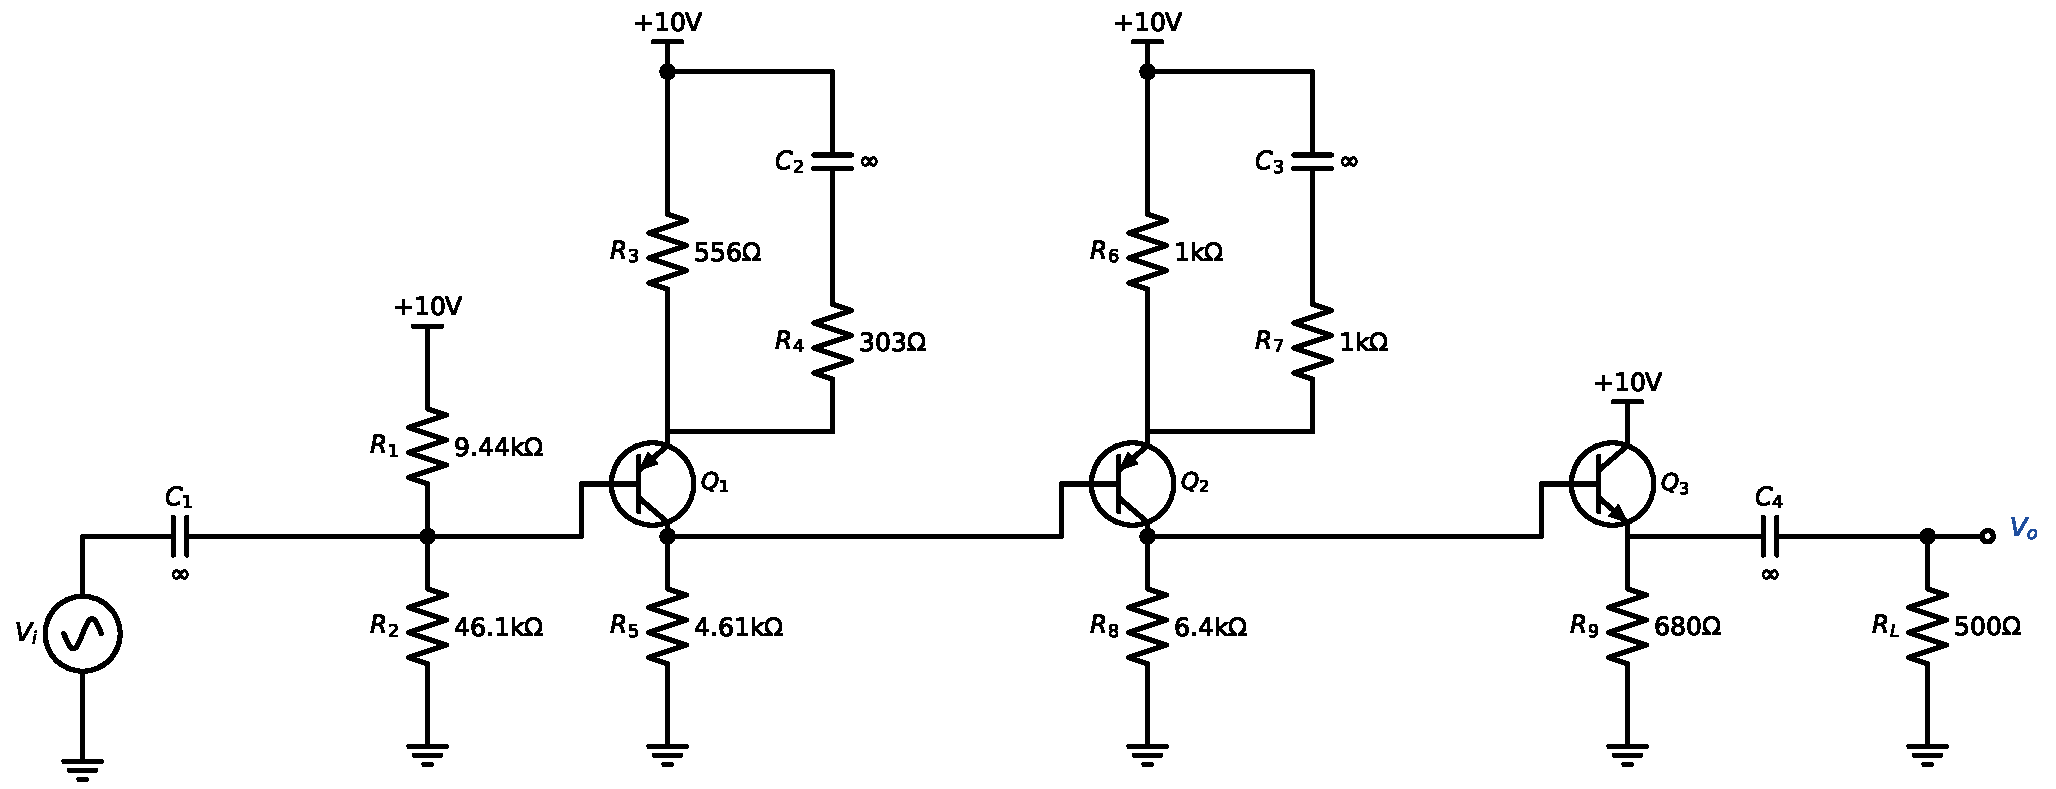
\includegraphics[width=0.9\linewidth,height=6.5cm,keepaspectratio]{p14_designed}\end{center}

\begin{ansbox}
$R_{1} = 9.44\,\mathrm{k}\Omega$,\quad $R_{2} = 46.1\,\mathrm{k}\Omega$,\quad $R_{3} = 556\,\Omega$,\quad $R_{4} = 303\,\Omega$,\quad $R_{5} = 4.61\,\mathrm{k}\Omega$,\quad $R_{6} = 1\,\mathrm{k}\Omega$,\quad $R_{7} = 1\,\mathrm{k}\Omega$,\quad $R_{8} = 6.4\,\mathrm{k}\Omega$,\quad $R_{9} = 680\,\Omega$
\end{ansbox}

\newpage
\subsection*{Solution 4E.15 \hfill Hard}
\begin{center}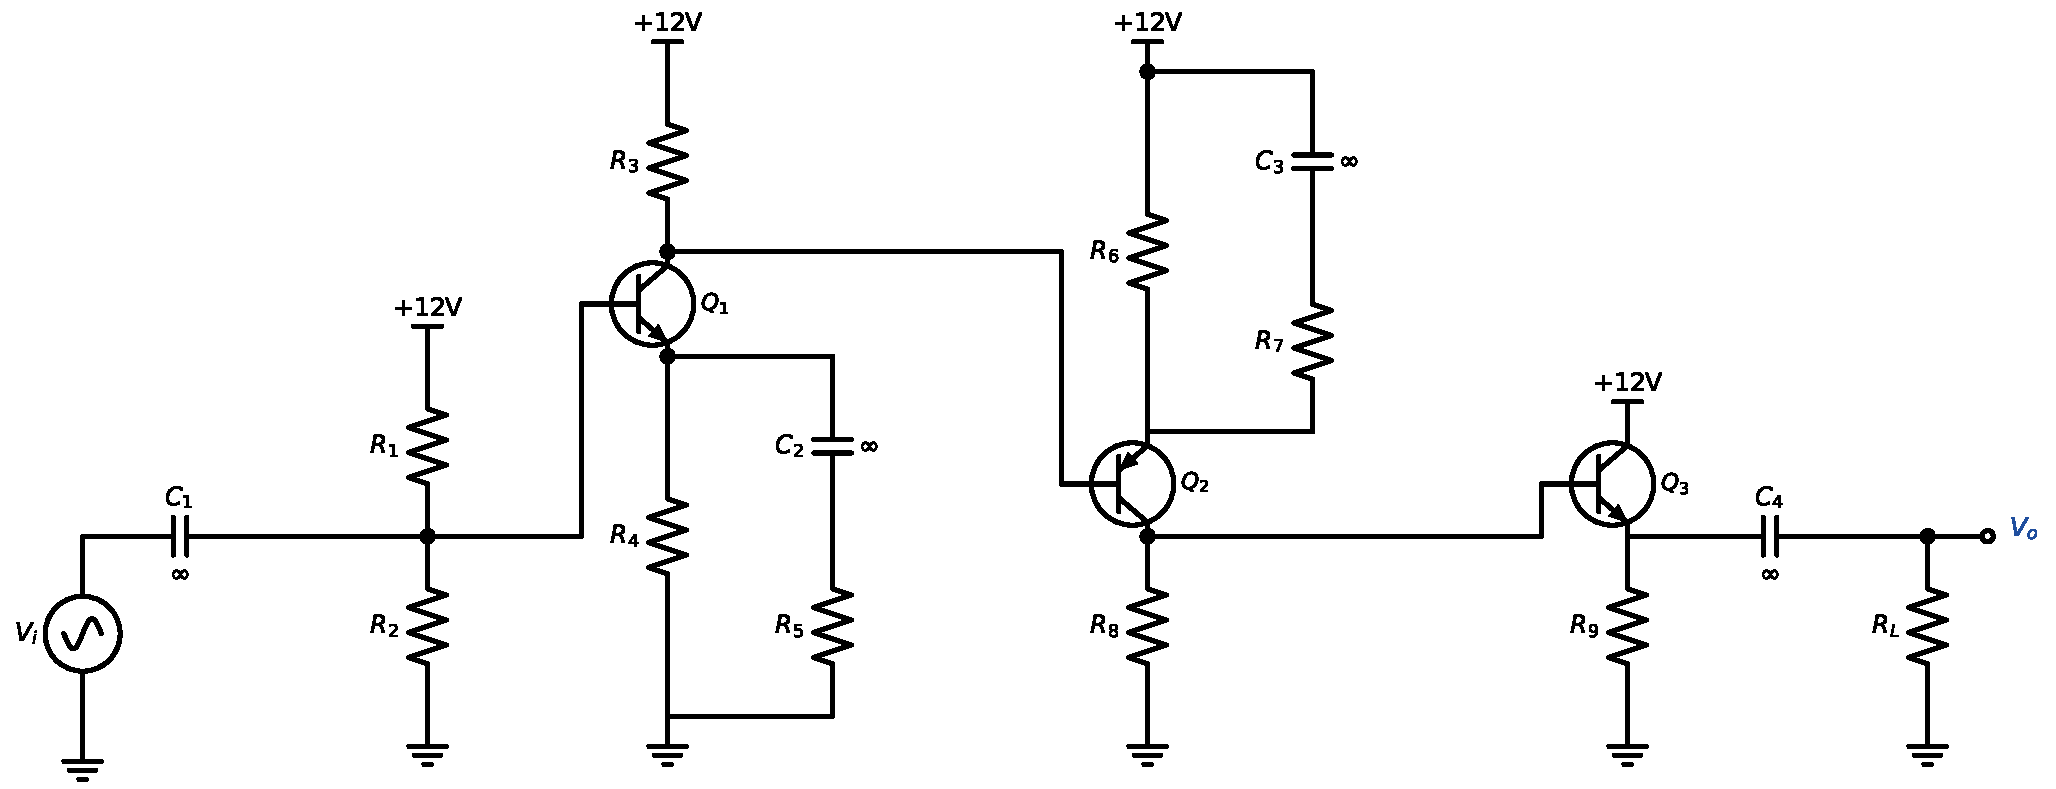
\includegraphics[width=0.9\linewidth,height=6cm,keepaspectratio]{p15_circuit}\end{center}
\solstep{1}{Plan}Name the resistors by their job: $R_{1} = R_{B1}$, $R_{2} = R_{B2}$, $R_{3} = R_{C1}$, $R_{4} = R_{E1}$, $R_{5} = R_{G1}$, $R_{6} = R_{E2}$, $R_{7} = R_{G2}$, $R_{8} = R_{C2}$, $R_{9} = R_H$. Every stage is biased like the one-stage design of the slides: $V_{RE}\ge1$\,V ($V_{BE}$-insensitive), the divider and every collector current much larger than the base current it feeds ($\beta$-insensitive, factor $N$), and $V_{RC}$ as large as the swing allows. Small-signal tools: $r_e = V_T/I_C$, CE gain $|A_v| = \frac{Z_C}{r_e + R_E\|R_G}$, follower gain $\frac{Z_E}{r_e+Z_E}$, base resistance $(\beta+1)(r_e + Z_E)$ (the $\infty$ capacitors put $R_G$ in parallel with $R_E$ for AC only). Design from the output back to the input, because each stage loads the one before it.
\solstep{2}{Output stage and follower}$V_{BE}$-insensitive: $V_{RE2} \ge 1$\,V; use $V_{RE2} = 1$\,V.

Collector swing of $Q_{2}$: about $\hat V_o$ (the follower has a gain close to 1). Largest $V_{RC2}$ without clipping: \[V_{RC2} = V_{CC} - \hat V_o - V_{RE2} - V_{CE,sat} = 12 - 2.4 - 1 - 0.2 = 8.4\,\mathrm{V}\]

Follower $Q_{3}$: its emitter sits at $0.7$\,V from the collector of $Q_{2}$, so $V_{RH} = V_{RC2} - 0.7 = 7.7\,\mathrm{V}$. To avoid current clipping the DC current in $R_H$ must stay larger than the peak current pushed into $R_L$: \[\frac{V_{RC2} - 0.7 - \hat V_o}{R_H} \ge \frac{\hat V_o}{R_L} \Rightarrow R_H \le R_L\frac{V_{RC2} - 0.7 - \hat V_o}{\hat V_o} = 1\,\mathrm{k}\Omega\cdot\frac{7.7 - 2.4}{2.4} = 2.21\,\mathrm{k}\Omega\]Take the E12 value just below: $R_H = \mathbf{2.2\,\mathrm{k}\Omega}$. Then $I_{C3} \approx \frac{V_{RH}}{R_H} = \frac{7.7}{2.2\,\mathrm{k}\Omega} = 3.5\,\mathrm{m}\mathrm{A}$, $r_{e3} = \frac{V_T}{I_{C3}} = 7.14\,\Omega$, and with $R_H \| R_L = 688\,\Omega$:\[A_{v3} = \frac{R_H\|R_L}{r_{e3} + R_H\|R_L} = 0.9897,\qquad R_{i3} = (\beta+1)(r_{e3} + R_H\|R_L) = 70.2\,\mathrm{k}\Omega\]
\solstep{3}{Stage 2 (common emitter, $Q_{2}$)}$\beta$-insensitive: $I_{C2} \ge N\frac{I_{C3}}{\beta} = 20\cdot\frac{3.5\,\mathrm{m}\mathrm{A}}{100} = 700\,\mu \mathrm{A}$; take the E12 value just above, $I_{C2} = 820\,\mu \mathrm{A}$.

\[R_{C2} = \frac{V_{RC2}}{I_{C2}} = \frac{8.4}{820\,\mu \mathrm{A}} = \mathbf{10.2\,\mathrm{k}\Omega},\quad R_{E2} = \frac{V_{RE2}}{I_{C2}} = \frac{1}{820\,\mu \mathrm{A}} = \mathbf{1.22\,\mathrm{k}\Omega},\quad r_{e2} = \frac{V_T}{I_{C2}} = 30.5\,\Omega\]

Gain $|A_{v2}| = \frac{R_{C2}\|R_{i3}}{r_{e2} + R_{E2}\|R_{G2}} = 8$ with $R_{C2}\|R_{i3} = 8.94\,\mathrm{k}\Omega$:\[R_{E2}\|R_{G2} = \frac{R_{C2}\|R_{i3}}{|A_{v2}|} - r_{e2} = 1.09\,\mathrm{k}\Omega \;\Rightarrow\; R_{G2} = \frac{1}{\frac{1}{1.09\,\mathrm{k}\Omega} - \frac{1}{1.22\,\mathrm{k}\Omega}} = \mathbf{9.99\,\mathrm{k}\Omega}\]

Its input resistance: $R_{i2} = (\beta+1)(r_{e2} + R_{E2}\|R_{G2}) = 113\,\mathrm{k}\Omega$.
\solstep{4}{Input stage ($Q_1$)}Gain left for stage 1: $|A_{v1}| = \frac{|A_v|}{|A_{v2}| A_{v3}} = \frac{150}{7.918} = 18.94$. The base of $Q_2$ fixes the collector of $Q_1$: $V_{RC1} = 1.7\,\mathrm{V}$. Its collector swing is only $\hat V_o/(\text{gain after it}) = 0.3031\,\mathrm{V}$, so $V_{RE1} \le V_{CC} - V_{RC1} - V_{CE,sat} - 0.303 = 9.797\,\mathrm{V}$; with $V_{RE1} \ge 1$\,V use $V_{RE1} = 1.5$\,V.

Divider: $V_{RB2} = V_{B1} = 2.2\,\mathrm{V}$, $V_{RB1} = V_{CC} - V_{B1} = 9.8\,\mathrm{V}$ ($|V_{RE1}| + 0.7$ on the emitter side). $\beta$-insensitive: the divider current is $N$ times the base current, $I_{RB} = N\frac{I_{C1}}{\beta}$, $N = 20$. Input resistance (all three in parallel, with $(\beta+1)(r_e + R_E\|R_G) \approx \beta\frac{R_{C1}}{|A_{v1}|} = \beta\frac{V_{RC1}}{I_{C1}|A_{v1}|}$):\[R_i \approx \frac{\beta/I_{C1}}{\frac{N}{V_{RB1}} + \frac{N}{V_{RB2}} + \frac{|A_{v1}|}{V_{RC1}}} \ge R_{i,spec} \;\Rightarrow\; I_{C1} \le \frac{\beta/R_{i,spec}}{\frac{20}{9.8} + \frac{20}{2.2} + \frac{18.94}{1.7}} = 1.12\,\mathrm{m}\mathrm{A}\]Take the E12 value just below: $I_{C1} = 1\,\mathrm{m}\mathrm{A}$. 

Check $I_{C1} \ge N\frac{I_{C2}}{\beta} = 164\,\mu \mathrm{A}$ \checkmark. 

\[R_{C1} = \frac{V_{RC1}}{I_{C1}} = \frac{1.7}{1\,\mathrm{m}\mathrm{A}} = \mathbf{1.7\,\mathrm{k}\Omega},\quad R_{E1} = \frac{V_{RE1}}{I_{C1}} = \frac{1.5}{1\,\mathrm{m}\mathrm{A}} = \mathbf{1.5\,\mathrm{k}\Omega},\quad r_{e1} = \frac{V_T}{I_{C1}} = 25\,\Omega\]

Gain $|A_{v1}| = \frac{R_{C1}\|R_{i2}}{r_{e1} + R_{E1}\|R_{G1}} = 18.94$ with $R_{C1}\|R_{i2} = 1.67\,\mathrm{k}\Omega$:\[R_{E1}\|R_{G1} = \frac{R_{C1}\|R_{i2}}{|A_{v1}|} - r_{e1} = 63.4\,\Omega \;\Rightarrow\; R_{G1} = \frac{1}{\frac{1}{63.4\,\Omega} - \frac{1}{1.5\,\mathrm{k}\Omega}} = \mathbf{66.2\,\Omega}\]

\[R_{B1} = \frac{V_{RB1}}{N I_{C1}/\beta} = \frac{9.8}{200\,\mu \mathrm{A}} = \mathbf{49\,\mathrm{k}\Omega},\qquad R_{B2} = \frac{V_{RB2}}{N I_{C1}/\beta} = \frac{2.2}{200\,\mu \mathrm{A}} = \mathbf{11\,\mathrm{k}\Omega}\]

Check: $R_i = R_{B1}\|R_{B2}\|(\beta+1)(r_{e1} + R_{E1}\|R_{G1}) = 49\,\mathrm{k}\Omega\|11\,\mathrm{k}\Omega\|8.93\,\mathrm{k}\Omega = 4.478\,\mathrm{k}\Omega$ $\ge 4\,\mathrm{k}\Omega$ \checkmark.
\solstep{5}{Check by analysis}Solve the finished circuit exactly ($\beta=100$, base currents included) for the DC point, then the small-signal gain with the exact $r_e$ values:\begin{center}\renewcommand{\arraystretch}{1.35}
\begin{tabular}{cccc}
\toprule
 & design $I_C$ & exact $I_C$ & exact $|V_{CE}|$ \\
\midrule
$Q_{1}$ & $1\,\mathrm{m}\mathrm{A}$ & $935\,\mu \mathrm{A}$ & $9.007\,\mathrm{V}$ \\
$Q_{2}$ & $820\,\mu \mathrm{A}$ & $712\,\mu \mathrm{A}$ & $4.121\,\mathrm{V}$ \\
$Q_{3}$ & $3.5\,\mathrm{m}\mathrm{A}$ & $2.84\,\mathrm{m}\mathrm{A}$ & $5.698\,\mathrm{V}$ \\
\bottomrule
\end{tabular}\end{center}
The exact currents are a little off the design values: $N$ only makes each base current $N$ times smaller than the current it disturbs, so the base voltages sag slightly, and along direct-coupled stages each shift is passed on (and amplified) to the next stage. The slides handle this the same way: simulate, then adjust. The exact gain is $|A_v| = 143.3$ instead of $150$ (the hand design ignored $\alpha$ and the base currents). As the slides suggest, trim $R_{G1}$: the gain is proportional to $1/(r_{e1} + R_{E1}\|R_{G1})$, so scale that sum by $143.3/150$ (exact $r_{e1} = 26.7\,\Omega$):\[R_{E1}\|R_{G1} = (26.7\,\Omega + 63.4\,\Omega)\frac{143.3}{150} - 26.7\,\Omega = 59.4\,\Omega \;\Rightarrow\; R_{G1} = \mathbf{61.8\,\Omega}\]Re-analysis: $|A_v| = 150$ \checkmark. \par The follower would clip at $\hat V_o = I_{E3}(R_H\|R_L) = 2.84\,\mathrm{m}\mathrm{A}\times688\,\Omega = 1.95\,\mathrm{V} < 2$\,V: its exact current is below the design value because the base currents shift the DC voltages along the direct-coupled chain. Adjust: lower $R_H$ to the next E12 value, $R_H = \mathbf{1.8\,\mathrm{k}\Omega}$ (more follower current), and analyse again. The exact gain is $|A_v| = 148.9$ instead of $150$ (the hand design ignored $\alpha$ and the base currents). As the slides suggest, trim $R_{G1}$: the gain is proportional to $1/(r_{e1} + R_{E1}\|R_{G1})$, so scale that sum by $148.9/150$ (exact $r_{e1} = 26.7\,\Omega$):\[R_{E1}\|R_{G1} = (26.7\,\Omega + 59.4\,\Omega)\frac{148.9}{150} - 26.7\,\Omega = 58.7\,\Omega \;\Rightarrow\; R_{G1} = \mathbf{61.1\,\Omega}\]Re-analysis: $|A_v| = 150$ \checkmark. \begin{itemize}[leftmargin=*,itemsep=2pt]
\item Input resistance (exact): $R_i = 4.4\,\mathrm{k}\Omega$ $\ge 4\,\mathrm{k}\Omega$ \checkmark
\item Output swing: follower current clipping at $\hat V_o = I_{E3}(R_H\|R_L) = 2.36\,\mathrm{V}$; $Q_{2}$ clips (saturation or cutoff) at $\hat V_o = 3.94\,\mathrm{V}$; $Q_{1}$ clips (saturation or cutoff) at $\hat V_o = 12.22\,\mathrm{V}$. The smallest, $2.36\,\mathrm{V}$, is $\ge 2$\,V \checkmark
\item Distortion: each CE stage adds $HD_2 \approx \frac{\hat v_b}{4V_T}\left(\frac{r_e}{r_e + R_E\|R_G}\right)^2$ ($\hat v_b$ = its input amplitude at the specified output; for one stage this is the slides' $\frac{\hat V_o V_T |A_v|}{4V_{RC}^2}$): THD $\approx 1.2 + 0.24\,\% = 1.4\,\%$ $\le 5\,\%$ \checkmark
\item $V_{BE}$-insensitive: $V_{RE1} = 1.5$\,V, $V_{RE2} = 1$\,V $\ge 1$\,V \checkmark
\end{itemize}

\begin{center}\renewcommand{\arraystretch}{1.35}
\begin{tabular}{ll}
\toprule
resistor & value \\
\midrule
$R_{1}$ ($R_{B1}$) & $49\,\mathrm{k}\Omega$ \\
$R_{2}$ ($R_{B2}$) & $11\,\mathrm{k}\Omega$ \\
$R_{3}$ ($R_{C1}$) & $1.7\,\mathrm{k}\Omega$ \\
$R_{4}$ ($R_{E1}$) & $1.5\,\mathrm{k}\Omega$ \\
$R_{5}$ ($R_{G1}$) & $61.1\,\Omega$ \\
$R_{6}$ ($R_{E2}$) & $1.22\,\mathrm{k}\Omega$ \\
$R_{7}$ ($R_{G2}$) & $9.99\,\mathrm{k}\Omega$ \\
$R_{8}$ ($R_{C2}$) & $10.2\,\mathrm{k}\Omega$ \\
$R_{9}$ ($R_H$) & $1.8\,\mathrm{k}\Omega$ \\
\bottomrule
\end{tabular}\end{center}
\begin{center}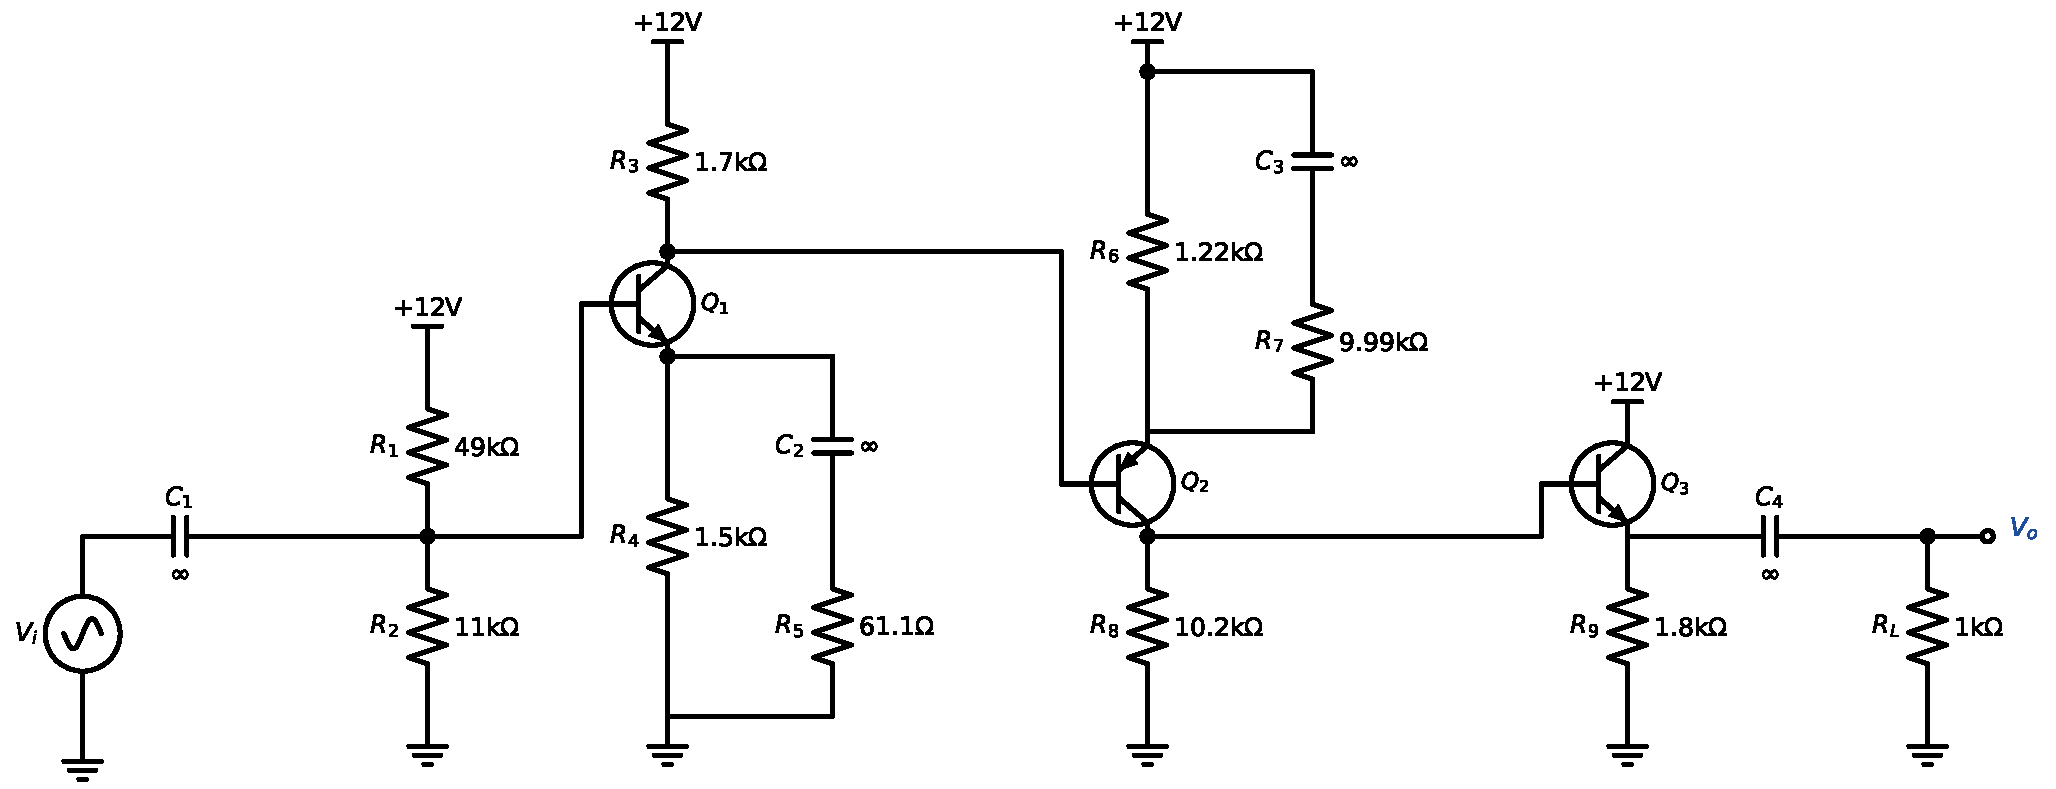
\includegraphics[width=0.9\linewidth,height=6.5cm,keepaspectratio]{p15_designed}\end{center}

\begin{ansbox}
$R_{1} = 49\,\mathrm{k}\Omega$,\quad $R_{2} = 11\,\mathrm{k}\Omega$,\quad $R_{3} = 1.7\,\mathrm{k}\Omega$,\quad $R_{4} = 1.5\,\mathrm{k}\Omega$,\quad $R_{5} = 61.1\,\Omega$,\quad $R_{6} = 1.22\,\mathrm{k}\Omega$,\quad $R_{7} = 9.99\,\mathrm{k}\Omega$,\quad $R_{8} = 10.2\,\mathrm{k}\Omega$,\quad $R_{9} = 1.8\,\mathrm{k}\Omega$
\end{ansbox}

\newpage
\subsection*{Solution 4E.16 \hfill Hard}
\begin{center}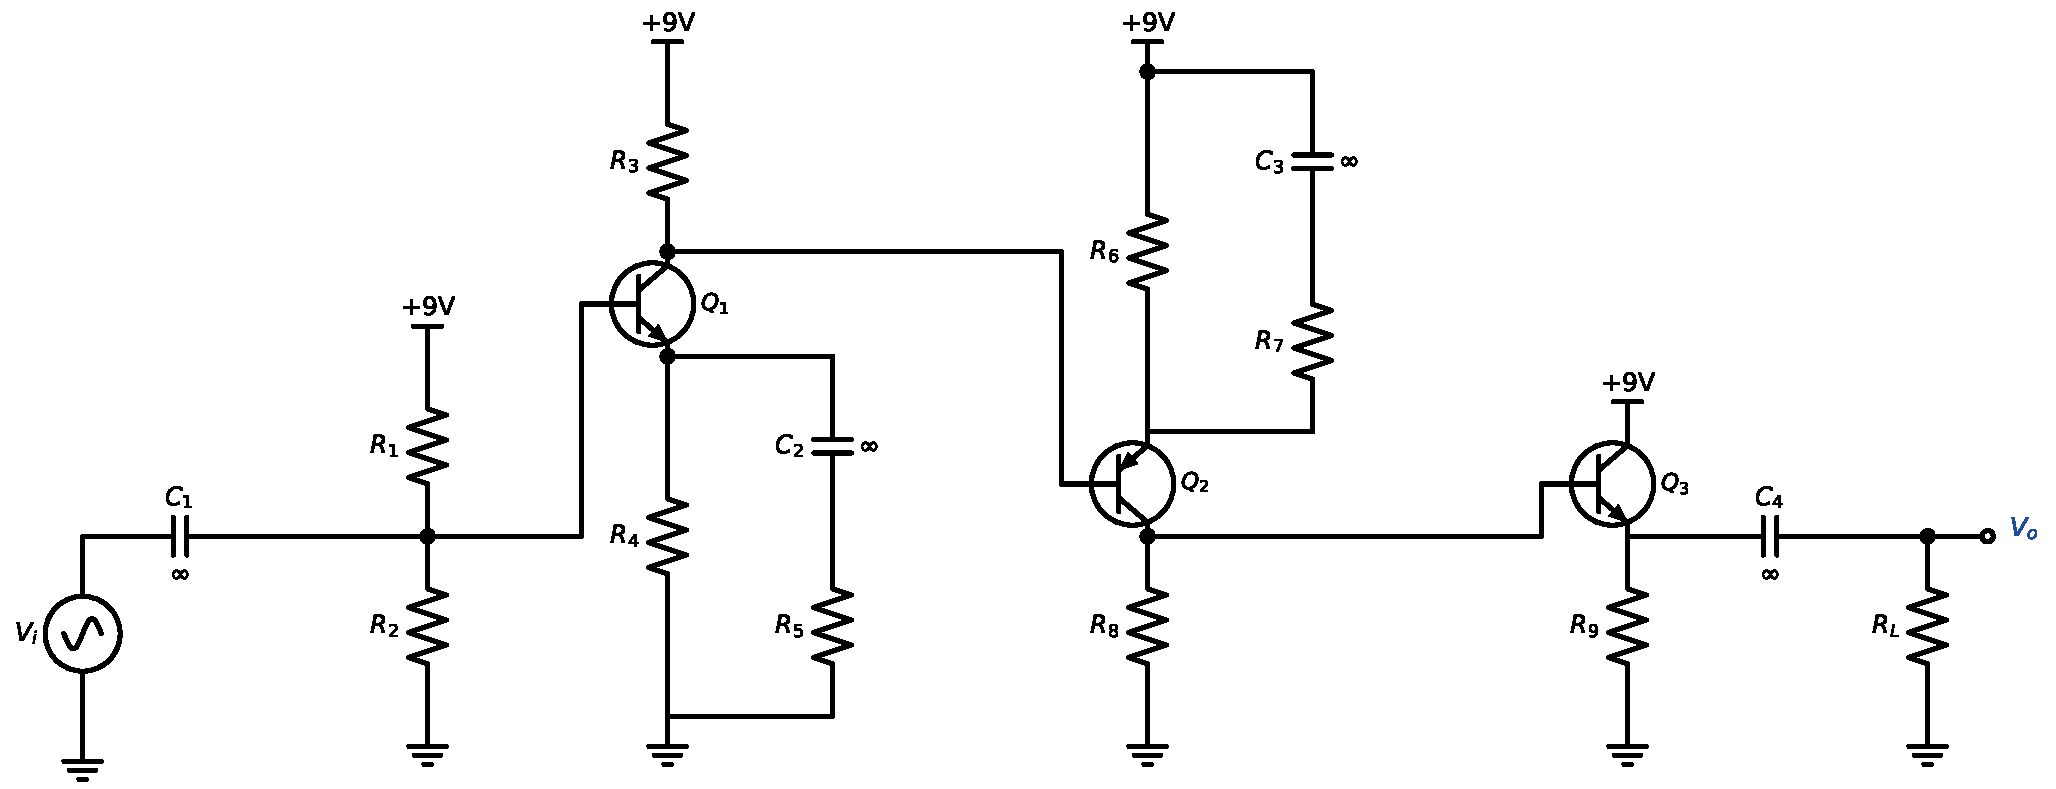
\includegraphics[width=0.9\linewidth,height=6cm,keepaspectratio]{p16_circuit}\end{center}
\solstep{1}{Plan}Name the resistors by their job: $R_{1} = R_{B1}$, $R_{2} = R_{B2}$, $R_{3} = R_{C1}$, $R_{4} = R_{E1}$, $R_{5} = R_{G1}$, $R_{6} = R_{E2}$, $R_{7} = R_{G2}$, $R_{8} = R_{C2}$, $R_{9} = R_H$. Every stage is biased like the one-stage design of the slides: $V_{RE}\ge1$\,V ($V_{BE}$-insensitive), the divider and every collector current much larger than the base current it feeds ($\beta$-insensitive, factor $N$), and $V_{RC}$ as large as the swing allows. Small-signal tools: $r_e = V_T/I_C$, CE gain $|A_v| = \frac{Z_C}{r_e + R_E\|R_G}$, follower gain $\frac{Z_E}{r_e+Z_E}$, base resistance $(\beta+1)(r_e + Z_E)$ (the $\infty$ capacitors put $R_G$ in parallel with $R_E$ for AC only). Design from the output back to the input, because each stage loads the one before it.
\solstep{2}{Output stage and follower}$V_{BE}$-insensitive: $V_{RE2} \ge 1$\,V; use $V_{RE2} = 1$\,V.

Collector swing of $Q_{2}$: about $\hat V_o$ (the follower has a gain close to 1). Largest $V_{RC2}$ without clipping: \[V_{RC2} = V_{CC} - \hat V_o - V_{RE2} - V_{CE,sat} = 9 - 1.8 - 1 - 0.2 = 6\,\mathrm{V}\]

Follower $Q_{3}$: its emitter sits at $0.7$\,V from the collector of $Q_{2}$, so $V_{RH} = V_{RC2} - 0.7 = 5.3\,\mathrm{V}$. To avoid current clipping the DC current in $R_H$ must stay larger than the peak current pushed into $R_L$: \[\frac{V_{RC2} - 0.7 - \hat V_o}{R_H} \ge \frac{\hat V_o}{R_L} \Rightarrow R_H \le R_L\frac{V_{RC2} - 0.7 - \hat V_o}{\hat V_o} = 300\,\Omega\cdot\frac{5.3 - 1.8}{1.8} = 583\,\Omega\]Take the E12 value just below: $R_H = \mathbf{560\,\Omega}$. Then $I_{C3} \approx \frac{V_{RH}}{R_H} = \frac{5.3}{560\,\Omega} = 9.46\,\mathrm{m}\mathrm{A}$, $r_{e3} = \frac{V_T}{I_{C3}} = 2.64\,\Omega$, and with $R_H \| R_L = 195\,\Omega$:\[A_{v3} = \frac{R_H\|R_L}{r_{e3} + R_H\|R_L} = 0.9867,\qquad R_{i3} = (\beta+1)(r_{e3} + R_H\|R_L) = 20\,\mathrm{k}\Omega\]
\solstep{3}{Stage 2 (common emitter, $Q_{2}$)}$\beta$-insensitive: $I_{C2} \ge N\frac{I_{C3}}{\beta} = 10\cdot\frac{9.46\,\mathrm{m}\mathrm{A}}{100} = 946\,\mu \mathrm{A}$; take the E12 value just above, $I_{C2} = 1\,\mathrm{m}\mathrm{A}$.

\[R_{C2} = \frac{V_{RC2}}{I_{C2}} = \frac{6}{1\,\mathrm{m}\mathrm{A}} = \mathbf{6\,\mathrm{k}\Omega},\quad R_{E2} = \frac{V_{RE2}}{I_{C2}} = \frac{1}{1\,\mathrm{m}\mathrm{A}} = \mathbf{1\,\mathrm{k}\Omega},\quad r_{e2} = \frac{V_T}{I_{C2}} = 25\,\Omega\]

Gain $|A_{v2}| = \frac{R_{C2}\|R_{i3}}{r_{e2} + R_{E2}\|R_{G2}} = 8$ with $R_{C2}\|R_{i3} = 4.62\,\mathrm{k}\Omega$:\[R_{E2}\|R_{G2} = \frac{R_{C2}\|R_{i3}}{|A_{v2}|} - r_{e2} = 552\,\Omega \;\Rightarrow\; R_{G2} = \frac{1}{\frac{1}{552\,\Omega} - \frac{1}{1\,\mathrm{k}\Omega}} = \mathbf{1.23\,\mathrm{k}\Omega}\]

Its input resistance: $R_{i2} = (\beta+1)(r_{e2} + R_{E2}\|R_{G2}) = 58.3\,\mathrm{k}\Omega$.
\solstep{4}{Input stage ($Q_1$)}Gain left for stage 1: $|A_{v1}| = \frac{|A_v|}{|A_{v2}| A_{v3}} = \frac{120}{7.893} = 15.2$. The base of $Q_2$ fixes the collector of $Q_1$: $V_{RC1} = 1.7\,\mathrm{V}$. Its collector swing is only $\hat V_o/(\text{gain after it}) = 0.228\,\mathrm{V}$, so $V_{RE1} \le V_{CC} - V_{RC1} - V_{CE,sat} - 0.228 = 6.872\,\mathrm{V}$; with $V_{RE1} \ge 1$\,V use $V_{RE1} = 1$\,V.

Divider: $V_{RB2} = V_{B1} = 1.7\,\mathrm{V}$, $V_{RB1} = V_{CC} - V_{B1} = 7.3\,\mathrm{V}$ ($|V_{RE1}| + 0.7$ on the emitter side). $\beta$-insensitive: the divider current is $N$ times the base current, $I_{RB} = N\frac{I_{C1}}{\beta}$, $N = 10$. Input resistance (all three in parallel, with $(\beta+1)(r_e + R_E\|R_G) \approx \beta\frac{R_{C1}}{|A_{v1}|} = \beta\frac{V_{RC1}}{I_{C1}|A_{v1}|}$):\[R_i \approx \frac{\beta/I_{C1}}{\frac{N}{V_{RB1}} + \frac{N}{V_{RB2}} + \frac{|A_{v1}|}{V_{RC1}}} \ge R_{i,spec} \;\Rightarrow\; I_{C1} \le \frac{\beta/R_{i,spec}}{\frac{10}{7.3} + \frac{10}{1.7} + \frac{15.2}{1.7}} = 2.06\,\mathrm{m}\mathrm{A}\]Take the E12 value just below: $I_{C1} = 1.8\,\mathrm{m}\mathrm{A}$. 

Check $I_{C1} \ge N\frac{I_{C2}}{\beta} = 100\,\mu \mathrm{A}$ \checkmark. 

\[R_{C1} = \frac{V_{RC1}}{I_{C1}} = \frac{1.7}{1.8\,\mathrm{m}\mathrm{A}} = \mathbf{944\,\Omega},\quad R_{E1} = \frac{V_{RE1}}{I_{C1}} = \frac{1}{1.8\,\mathrm{m}\mathrm{A}} = \mathbf{556\,\Omega},\quad r_{e1} = \frac{V_T}{I_{C1}} = 13.9\,\Omega\]

Gain $|A_{v1}| = \frac{R_{C1}\|R_{i2}}{r_{e1} + R_{E1}\|R_{G1}} = 15.2$ with $R_{C1}\|R_{i2} = 929\,\Omega$:\[R_{E1}\|R_{G1} = \frac{R_{C1}\|R_{i2}}{|A_{v1}|} - r_{e1} = 47.2\,\Omega \;\Rightarrow\; R_{G1} = \frac{1}{\frac{1}{47.2\,\Omega} - \frac{1}{556\,\Omega}} = \mathbf{51.6\,\Omega}\]

\[R_{B1} = \frac{V_{RB1}}{N I_{C1}/\beta} = \frac{7.3}{180\,\mu \mathrm{A}} = \mathbf{40.6\,\mathrm{k}\Omega},\qquad R_{B2} = \frac{V_{RB2}}{N I_{C1}/\beta} = \frac{1.7}{180\,\mu \mathrm{A}} = \mathbf{9.44\,\mathrm{k}\Omega}\]

Check: $R_i = R_{B1}\|R_{B2}\|(\beta+1)(r_{e1} + R_{E1}\|R_{G1}) = 40.6\,\mathrm{k}\Omega\|9.44\,\mathrm{k}\Omega\|6.17\,\mathrm{k}\Omega = 3.419\,\mathrm{k}\Omega$ $\ge 3\,\mathrm{k}\Omega$ \checkmark.
\solstep{5}{Check by analysis}Solve the finished circuit exactly ($\beta=100$, base currents included) for the DC point, then the small-signal gain with the exact $r_e$ values:\begin{center}\renewcommand{\arraystretch}{1.35}
\begin{tabular}{cccc}
\toprule
 & design $I_C$ & exact $I_C$ & exact $|V_{CE}|$ \\
\midrule
$Q_{1}$ & $1.8\,\mathrm{m}\mathrm{A}$ & $1.57\,\mathrm{m}\mathrm{A}$ & $6.646\,\mathrm{V}$ \\
$Q_{2}$ & $1\,\mathrm{m}\mathrm{A}$ & $766\,\mu \mathrm{A}$ & $4.003\,\mathrm{V}$ \\
$Q_{3}$ & $9.46\,\mathrm{m}\mathrm{A}$ & $6.23\,\mathrm{m}\mathrm{A}$ & $5.477\,\mathrm{V}$ \\
\bottomrule
\end{tabular}\end{center}
The exact currents are a little off the design values: $N$ only makes each base current $N$ times smaller than the current it disturbs, so the base voltages sag slightly, and along direct-coupled stages each shift is passed on (and amplified) to the next stage. The slides handle this the same way: simulate, then adjust. The exact gain is $|A_v| = 111.8$ instead of $120$ (the hand design ignored $\alpha$ and the base currents). As the slides suggest, trim $R_{G1}$: the gain is proportional to $1/(r_{e1} + R_{E1}\|R_{G1})$, so scale that sum by $111.8/120$ (exact $r_{e1} = 15.9\,\Omega$):\[R_{E1}\|R_{G1} = (15.9\,\Omega + 47.2\,\Omega)\frac{111.8}{120} - 15.9\,\Omega = 42.9\,\Omega \;\Rightarrow\; R_{G1} = \mathbf{46.5\,\Omega}\]Re-analysis: $|A_v| = 120$ \checkmark. \par The follower would clip at $\hat V_o = I_{E3}(R_H\|R_L) = 6.23\,\mathrm{m}\mathrm{A}\times195\,\Omega = 1.217\,\mathrm{V} < 1.5$\,V: its exact current is below the design value because the base currents shift the DC voltages along the direct-coupled chain. Adjust: lower $R_H$ to the next E12 value, $R_H = \mathbf{470\,\Omega}$ (more follower current), and analyse again. The exact gain is $|A_v| = 118.3$ instead of $120$ (the hand design ignored $\alpha$ and the base currents). As the slides suggest, trim $R_{G1}$: the gain is proportional to $1/(r_{e1} + R_{E1}\|R_{G1})$, so scale that sum by $118.3/120$ (exact $r_{e1} = 15.9\,\Omega$):\[R_{E1}\|R_{G1} = (15.9\,\Omega + 42.9\,\Omega)\frac{118.3}{120} - 15.9\,\Omega = 42.1\,\Omega \;\Rightarrow\; R_{G1} = \mathbf{45.5\,\Omega}\]Re-analysis: $|A_v| = 120$ \checkmark. \par The follower would clip at $\hat V_o = I_{E3}(R_H\|R_L) = 7.29\,\mathrm{m}\mathrm{A}\times183\,\Omega = 1.424\,\mathrm{V} < 1.5$\,V: its exact current is below the design value because the base currents shift the DC voltages along the direct-coupled chain. Adjust: lower $R_H$ to the next E12 value, $R_H = \mathbf{390\,\Omega}$ (more follower current), and analyse again. The exact gain is $|A_v| = 117.9$ instead of $120$ (the hand design ignored $\alpha$ and the base currents). As the slides suggest, trim $R_{G1}$: the gain is proportional to $1/(r_{e1} + R_{E1}\|R_{G1})$, so scale that sum by $117.9/120$ (exact $r_{e1} = 15.9\,\Omega$):\[R_{E1}\|R_{G1} = (15.9\,\Omega + 42.1\,\Omega)\frac{117.9}{120} - 15.9\,\Omega = 41.1\,\Omega \;\Rightarrow\; R_{G1} = \mathbf{44.3\,\Omega}\]Re-analysis: $|A_v| = 120$ \checkmark. \begin{itemize}[leftmargin=*,itemsep=2pt]
\item Input resistance (exact): $R_i = 3.29\,\mathrm{k}\Omega$ $\ge 3\,\mathrm{k}\Omega$ \checkmark
\item Output swing: follower current clipping at $\hat V_o = I_{E3}(R_H\|R_L) = 1.677\,\mathrm{V}$; $Q_{2}$ clips (saturation or cutoff) at $\hat V_o = 3.485\,\mathrm{V}$; $Q_{1}$ clips (saturation or cutoff) at $\hat V_o = 11.23\,\mathrm{V}$. The smallest, $1.677\,\mathrm{V}$, is $\ge 1.5$\,V \checkmark
\item Distortion: each CE stage adds $HD_2 \approx \frac{\hat v_b}{4V_T}\left(\frac{r_e}{r_e + R_E\|R_G}\right)^2$ ($\hat v_b$ = its input amplitude at the specified output; for one stage this is the slides' $\frac{\hat V_o V_T |A_v|}{4V_{RC}^2}$): THD $\approx 0.8 + 0.57\,\% = 1.4\,\%$ $\le 5\,\%$ \checkmark
\item $V_{BE}$-insensitive: $V_{RE1} = 1$\,V, $V_{RE2} = 1$\,V $\ge 1$\,V \checkmark
\end{itemize}

\begin{center}\renewcommand{\arraystretch}{1.35}
\begin{tabular}{ll}
\toprule
resistor & value \\
\midrule
$R_{1}$ ($R_{B1}$) & $40.6\,\mathrm{k}\Omega$ \\
$R_{2}$ ($R_{B2}$) & $9.44\,\mathrm{k}\Omega$ \\
$R_{3}$ ($R_{C1}$) & $944\,\Omega$ \\
$R_{4}$ ($R_{E1}$) & $556\,\Omega$ \\
$R_{5}$ ($R_{G1}$) & $44.3\,\Omega$ \\
$R_{6}$ ($R_{E2}$) & $1\,\mathrm{k}\Omega$ \\
$R_{7}$ ($R_{G2}$) & $1.23\,\mathrm{k}\Omega$ \\
$R_{8}$ ($R_{C2}$) & $6\,\mathrm{k}\Omega$ \\
$R_{9}$ ($R_H$) & $390\,\Omega$ \\
\bottomrule
\end{tabular}\end{center}
\begin{center}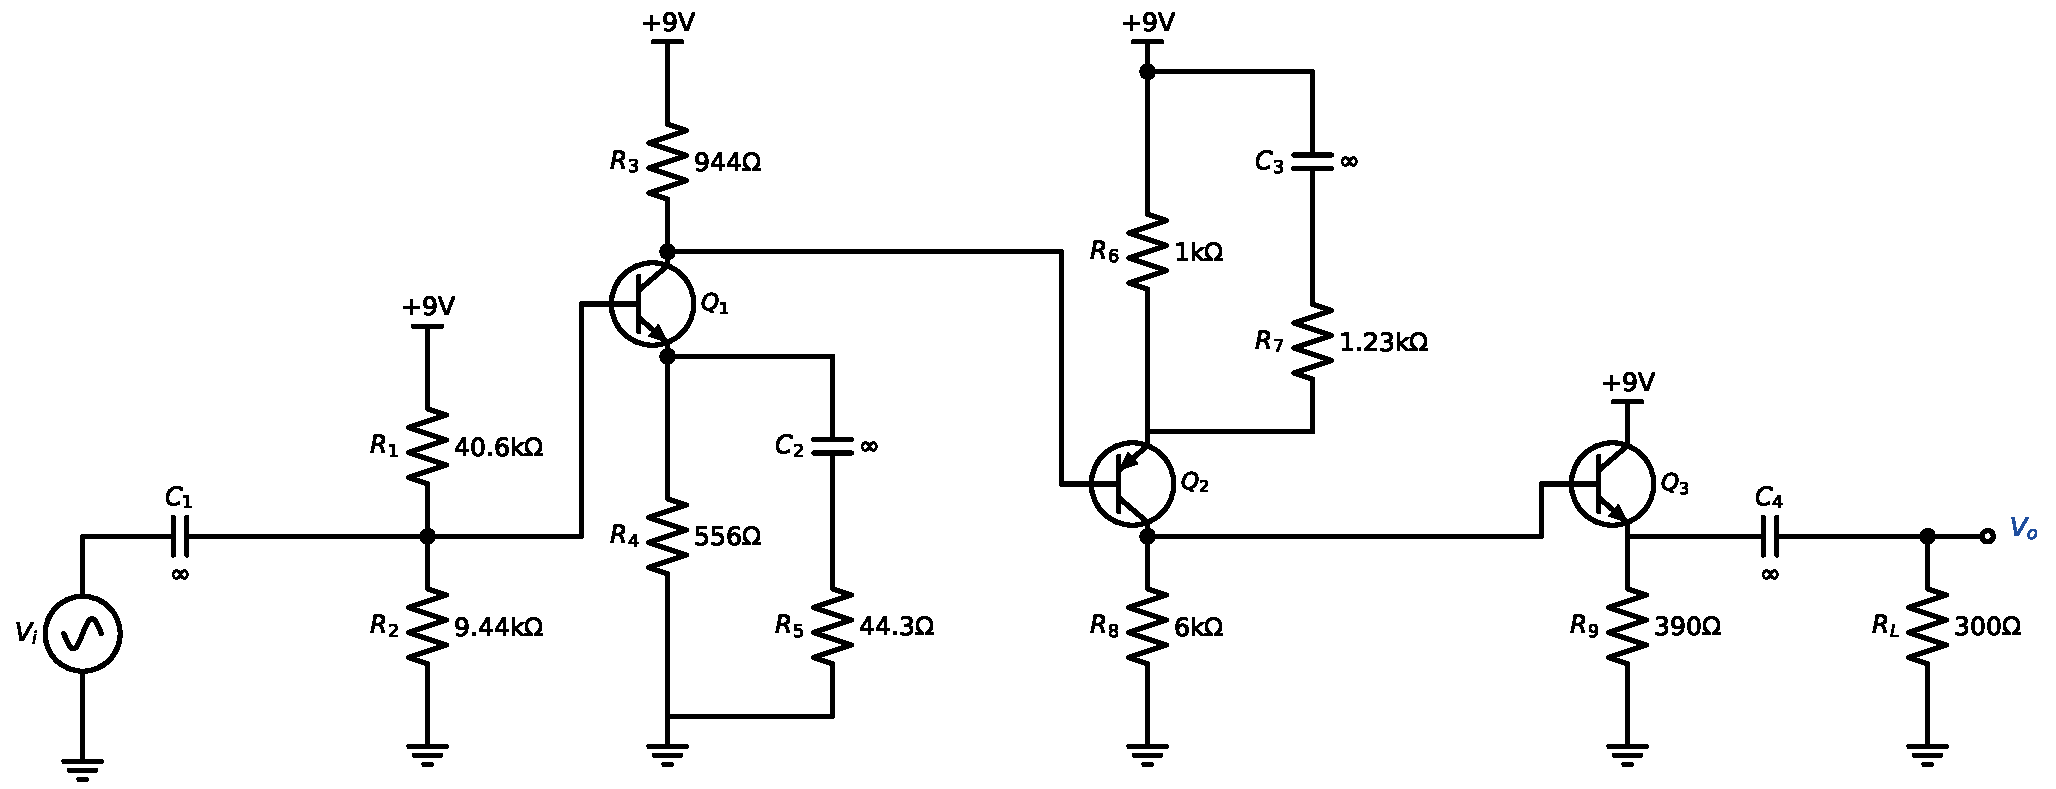
\includegraphics[width=0.9\linewidth,height=6.5cm,keepaspectratio]{p16_designed}\end{center}

\begin{ansbox}
$R_{1} = 40.6\,\mathrm{k}\Omega$,\quad $R_{2} = 9.44\,\mathrm{k}\Omega$,\quad $R_{3} = 944\,\Omega$,\quad $R_{4} = 556\,\Omega$,\quad $R_{5} = 44.3\,\Omega$,\quad $R_{6} = 1\,\mathrm{k}\Omega$,\quad $R_{7} = 1.23\,\mathrm{k}\Omega$,\quad $R_{8} = 6\,\mathrm{k}\Omega$,\quad $R_{9} = 390\,\Omega$
\end{ansbox}

\newpage
\subsection*{Solution 4E.17 \hfill Hard}
\begin{center}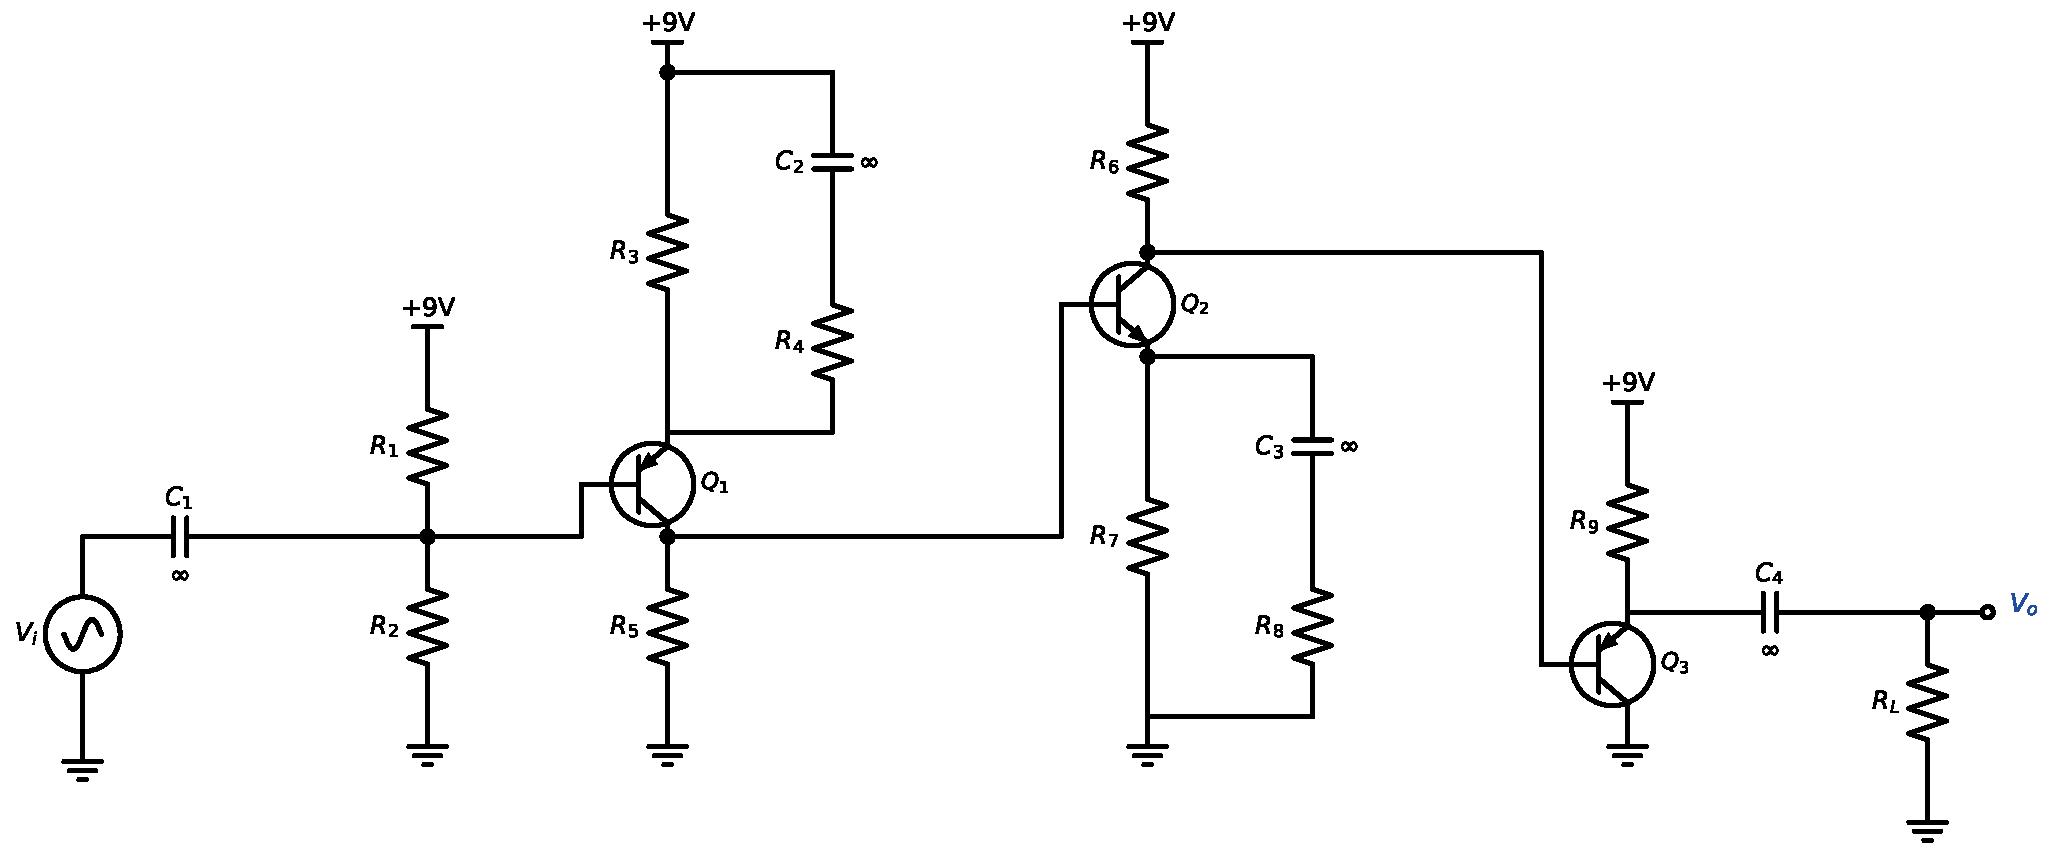
\includegraphics[width=0.9\linewidth,height=6cm,keepaspectratio]{p17_circuit}\end{center}
\solstep{1}{Plan}Name the resistors by their job: $R_{1} = R_{B1}$, $R_{2} = R_{B2}$, $R_{3} = R_{E1}$, $R_{4} = R_{G1}$, $R_{5} = R_{C1}$, $R_{6} = R_{C2}$, $R_{7} = R_{E2}$, $R_{8} = R_{G2}$, $R_{9} = R_H$. Every stage is biased like the one-stage design of the slides: $V_{RE}\ge1$\,V ($V_{BE}$-insensitive), the divider and every collector current much larger than the base current it feeds ($\beta$-insensitive, factor $N$), and $V_{RC}$ as large as the swing allows. Small-signal tools: $r_e = V_T/I_C$, CE gain $|A_v| = \frac{Z_C}{r_e + R_E\|R_G}$, follower gain $\frac{Z_E}{r_e+Z_E}$, base resistance $(\beta+1)(r_e + Z_E)$ (the $\infty$ capacitors put $R_G$ in parallel with $R_E$ for AC only). Design from the output back to the input, because each stage loads the one before it.
\solstep{2}{Output stage and follower}$V_{BE}$-insensitive: $V_{RE2} \ge 1$\,V; use $V_{RE2} = 1$\,V.

Collector swing of $Q_{2}$: about $\hat V_o$ (the follower has a gain close to 1). Largest $V_{RC2}$ without clipping: \[V_{RC2} = V_{CC} - \hat V_o - V_{RE2} - V_{CE,sat} = 9 - 2.5 - 1 - 0.2 = 5.3\,\mathrm{V}\]

Follower $Q_{3}$: its emitter sits at $0.7$\,V from the collector of $Q_{2}$, so $V_{RH} = V_{RC2} - 0.7 = 4.6\,\mathrm{V}$. To avoid current clipping the DC current in $R_H$ must stay larger than the peak current pushed into $R_L$: \[\frac{V_{RC2} - 0.7 - \hat V_o}{R_H} \ge \frac{\hat V_o}{R_L} \Rightarrow R_H \le R_L\frac{V_{RC2} - 0.7 - \hat V_o}{\hat V_o} = 200\,\Omega\cdot\frac{4.6 - 2.5}{2.5} = 168\,\Omega\]Take the E12 value just below: $R_H = \mathbf{150\,\Omega}$. Then $I_{C3} \approx \frac{V_{RH}}{R_H} = \frac{4.6}{150\,\Omega} = 30.7\,\mathrm{m}\mathrm{A}$, $r_{e3} = \frac{V_T}{I_{C3}} = 815\,\mathrm{m}\Omega$, and with $R_H \| R_L = 85.7\,\Omega$:\[A_{v3} = \frac{R_H\|R_L}{r_{e3} + R_H\|R_L} = 0.9906,\qquad R_{i3} = (\beta+1)(r_{e3} + R_H\|R_L) = 8.74\,\mathrm{k}\Omega\]
\solstep{3}{Stage 2 (common emitter, $Q_{2}$)}$\beta$-insensitive: $I_{C2} \ge N\frac{I_{C3}}{\beta} = 20\cdot\frac{30.7\,\mathrm{m}\mathrm{A}}{100} = 6.13\,\mathrm{m}\mathrm{A}$; take the E12 value just above, $I_{C2} = 6.8\,\mathrm{m}\mathrm{A}$.

\[R_{C2} = \frac{V_{RC2}}{I_{C2}} = \frac{5.3}{6.8\,\mathrm{m}\mathrm{A}} = \mathbf{779\,\Omega},\quad R_{E2} = \frac{V_{RE2}}{I_{C2}} = \frac{1}{6.8\,\mathrm{m}\mathrm{A}} = \mathbf{147\,\Omega},\quad r_{e2} = \frac{V_T}{I_{C2}} = 3.68\,\Omega\]

Gain $|A_{v2}| = \frac{R_{C2}\|R_{i3}}{r_{e2} + R_{E2}\|R_{G2}} = 8$ with $R_{C2}\|R_{i3} = 716\,\Omega$:\[R_{E2}\|R_{G2} = \frac{R_{C2}\|R_{i3}}{|A_{v2}|} - r_{e2} = 85.8\,\Omega \;\Rightarrow\; R_{G2} = \frac{1}{\frac{1}{85.8\,\Omega} - \frac{1}{147\,\Omega}} = \mathbf{206\,\Omega}\]

Its input resistance: $R_{i2} = (\beta+1)(r_{e2} + R_{E2}\|R_{G2}) = 9.03\,\mathrm{k}\Omega$.
\solstep{4}{Input stage ($Q_1$)}Gain left for stage 1: $|A_{v1}| = \frac{|A_v|}{|A_{v2}| A_{v3}} = \frac{150}{7.925} = 18.93$. The base of $Q_2$ fixes the collector of $Q_1$: $V_{RC1} = 1.7\,\mathrm{V}$. Its collector swing is only $\hat V_o/(\text{gain after it}) = 0.3155\,\mathrm{V}$, so $V_{RE1} \le V_{CC} - V_{RC1} - V_{CE,sat} - 0.315 = 6.785\,\mathrm{V}$; with $V_{RE1} \ge 1$\,V use $V_{RE1} = 1.5$\,V.

Divider: $V_{RB2} = V_{B1} = 6.8\,\mathrm{V}$, $V_{RB1} = V_{CC} - V_{B1} = 2.2\,\mathrm{V}$ ($|V_{RE1}| + 0.7$ on the emitter side). $\beta$-insensitive: the divider current is $N$ times the base current, $I_{RB} = N\frac{I_{C1}}{\beta}$, $N = 20$. Input resistance (all three in parallel, with $(\beta+1)(r_e + R_E\|R_G) \approx \beta\frac{R_{C1}}{|A_{v1}|} = \beta\frac{V_{RC1}}{I_{C1}|A_{v1}|}$):\[R_i \approx \frac{\beta/I_{C1}}{\frac{N}{V_{RB1}} + \frac{N}{V_{RB2}} + \frac{|A_{v1}|}{V_{RC1}}} \ge R_{i,spec} \;\Rightarrow\; I_{C1} \le \frac{\beta/R_{i,spec}}{\frac{20}{2.2} + \frac{20}{6.8} + \frac{18.93}{1.7}} = 2.16\,\mathrm{m}\mathrm{A}\]Take the E12 value just below: $I_{C1} = 1.8\,\mathrm{m}\mathrm{A}$. 

Check $I_{C1} \ge N\frac{I_{C2}}{\beta} = 1.36\,\mathrm{m}\mathrm{A}$ \checkmark. 

\[R_{C1} = \frac{V_{RC1}}{I_{C1}} = \frac{1.7}{1.8\,\mathrm{m}\mathrm{A}} = \mathbf{944\,\Omega},\quad R_{E1} = \frac{V_{RE1}}{I_{C1}} = \frac{1.5}{1.8\,\mathrm{m}\mathrm{A}} = \mathbf{833\,\Omega},\quad r_{e1} = \frac{V_T}{I_{C1}} = 13.9\,\Omega\]

Gain $|A_{v1}| = \frac{R_{C1}\|R_{i2}}{r_{e1} + R_{E1}\|R_{G1}} = 18.93$ with $R_{C1}\|R_{i2} = 855\,\Omega$:\[R_{E1}\|R_{G1} = \frac{R_{C1}\|R_{i2}}{|A_{v1}|} - r_{e1} = 31.3\,\Omega \;\Rightarrow\; R_{G1} = \frac{1}{\frac{1}{31.3\,\Omega} - \frac{1}{833\,\Omega}} = \mathbf{32.5\,\Omega}\]

\[R_{B1} = \frac{V_{RB1}}{N I_{C1}/\beta} = \frac{2.2}{360\,\mu \mathrm{A}} = \mathbf{6.11\,\mathrm{k}\Omega},\qquad R_{B2} = \frac{V_{RB2}}{N I_{C1}/\beta} = \frac{6.8}{360\,\mu \mathrm{A}} = \mathbf{18.9\,\mathrm{k}\Omega}\]

Check: $R_i = R_{B1}\|R_{B2}\|(\beta+1)(r_{e1} + R_{E1}\|R_{G1}) = 6.11\,\mathrm{k}\Omega\|18.9\,\mathrm{k}\Omega\|4.56\,\mathrm{k}\Omega = 2.295\,\mathrm{k}\Omega$ $\ge 2\,\mathrm{k}\Omega$ \checkmark.
\solstep{5}{Check by analysis}Solve the finished circuit exactly ($\beta=100$, base currents included) for the DC point, then the small-signal gain with the exact $r_e$ values:\begin{center}\renewcommand{\arraystretch}{1.35}
\begin{tabular}{cccc}
\toprule
 & design $I_C$ & exact $I_C$ & exact $|V_{CE}|$ \\
\midrule
$Q_{1}$ & $1.8\,\mathrm{m}\mathrm{A}$ & $1.69\,\mathrm{m}\mathrm{A}$ & $6.036\,\mathrm{V}$ \\
$Q_{2}$ & $6.8\,\mathrm{m}\mathrm{A}$ & $5.67\,\mathrm{m}\mathrm{A}$ & $3.921\,\mathrm{V}$ \\
$Q_{3}$ & $30.7\,\mathrm{m}\mathrm{A}$ & $23.3\,\mathrm{m}\mathrm{A}$ & $5.463\,\mathrm{V}$ \\
\bottomrule
\end{tabular}\end{center}
The exact currents are a little off the design values: $N$ only makes each base current $N$ times smaller than the current it disturbs, so the base voltages sag slightly, and along direct-coupled stages each shift is passed on (and amplified) to the next stage. The slides handle this the same way: simulate, then adjust. The exact gain is $|A_v| = 142.7$ instead of $150$ (the hand design ignored $\alpha$ and the base currents). As the slides suggest, trim $R_{G1}$: the gain is proportional to $1/(r_{e1} + R_{E1}\|R_{G1})$, so scale that sum by $142.7/150$ (exact $r_{e1} = 14.8\,\Omega$):\[R_{E1}\|R_{G1} = (14.8\,\Omega + 31.3\,\Omega)\frac{142.7}{150} - 14.8\,\Omega = 29\,\Omega \;\Rightarrow\; R_{G1} = \mathbf{30.1\,\Omega}\]Re-analysis: $|A_v| = 150$ \checkmark. \begin{itemize}[leftmargin=*,itemsep=2pt]
\item Input resistance (exact): $R_i = 2.26\,\mathrm{k}\Omega$ $\ge 2\,\mathrm{k}\Omega$ \checkmark
\item Output swing: follower current clipping at $\hat V_o = I_{E3}(R_H\|R_L) = 2.001\,\mathrm{V}$; $Q_{2}$ clips (saturation or cutoff) at $\hat V_o = 3.675\,\mathrm{V}$; $Q_{1}$ clips (saturation or cutoff) at $\hat V_o = 11.22\,\mathrm{V}$. The smallest, $2.001\,\mathrm{V}$, is $\ge 2$\,V \checkmark
\item Distortion: each CE stage adds $HD_2 \approx \frac{\hat v_b}{4V_T}\left(\frac{r_e}{r_e + R_E\|R_G}\right)^2$ ($\hat v_b$ = its input amplitude at the specified output; for one stage this is the slides' $\frac{\hat V_o V_T |A_v|}{4V_{RC}^2}$): THD $\approx 1.4 + 0.59\,\% = 2\,\%$ $\le 5\,\%$ \checkmark
\item $V_{BE}$-insensitive: $V_{RE1} = 1.5$\,V, $V_{RE2} = 1$\,V $\ge 1$\,V \checkmark
\end{itemize}

\begin{center}\renewcommand{\arraystretch}{1.35}
\begin{tabular}{ll}
\toprule
resistor & value \\
\midrule
$R_{1}$ ($R_{B1}$) & $6.11\,\mathrm{k}\Omega$ \\
$R_{2}$ ($R_{B2}$) & $18.9\,\mathrm{k}\Omega$ \\
$R_{3}$ ($R_{E1}$) & $833\,\Omega$ \\
$R_{4}$ ($R_{G1}$) & $30.1\,\Omega$ \\
$R_{5}$ ($R_{C1}$) & $944\,\Omega$ \\
$R_{6}$ ($R_{C2}$) & $779\,\Omega$ \\
$R_{7}$ ($R_{E2}$) & $147\,\Omega$ \\
$R_{8}$ ($R_{G2}$) & $206\,\Omega$ \\
$R_{9}$ ($R_H$) & $150\,\Omega$ \\
\bottomrule
\end{tabular}\end{center}
\begin{center}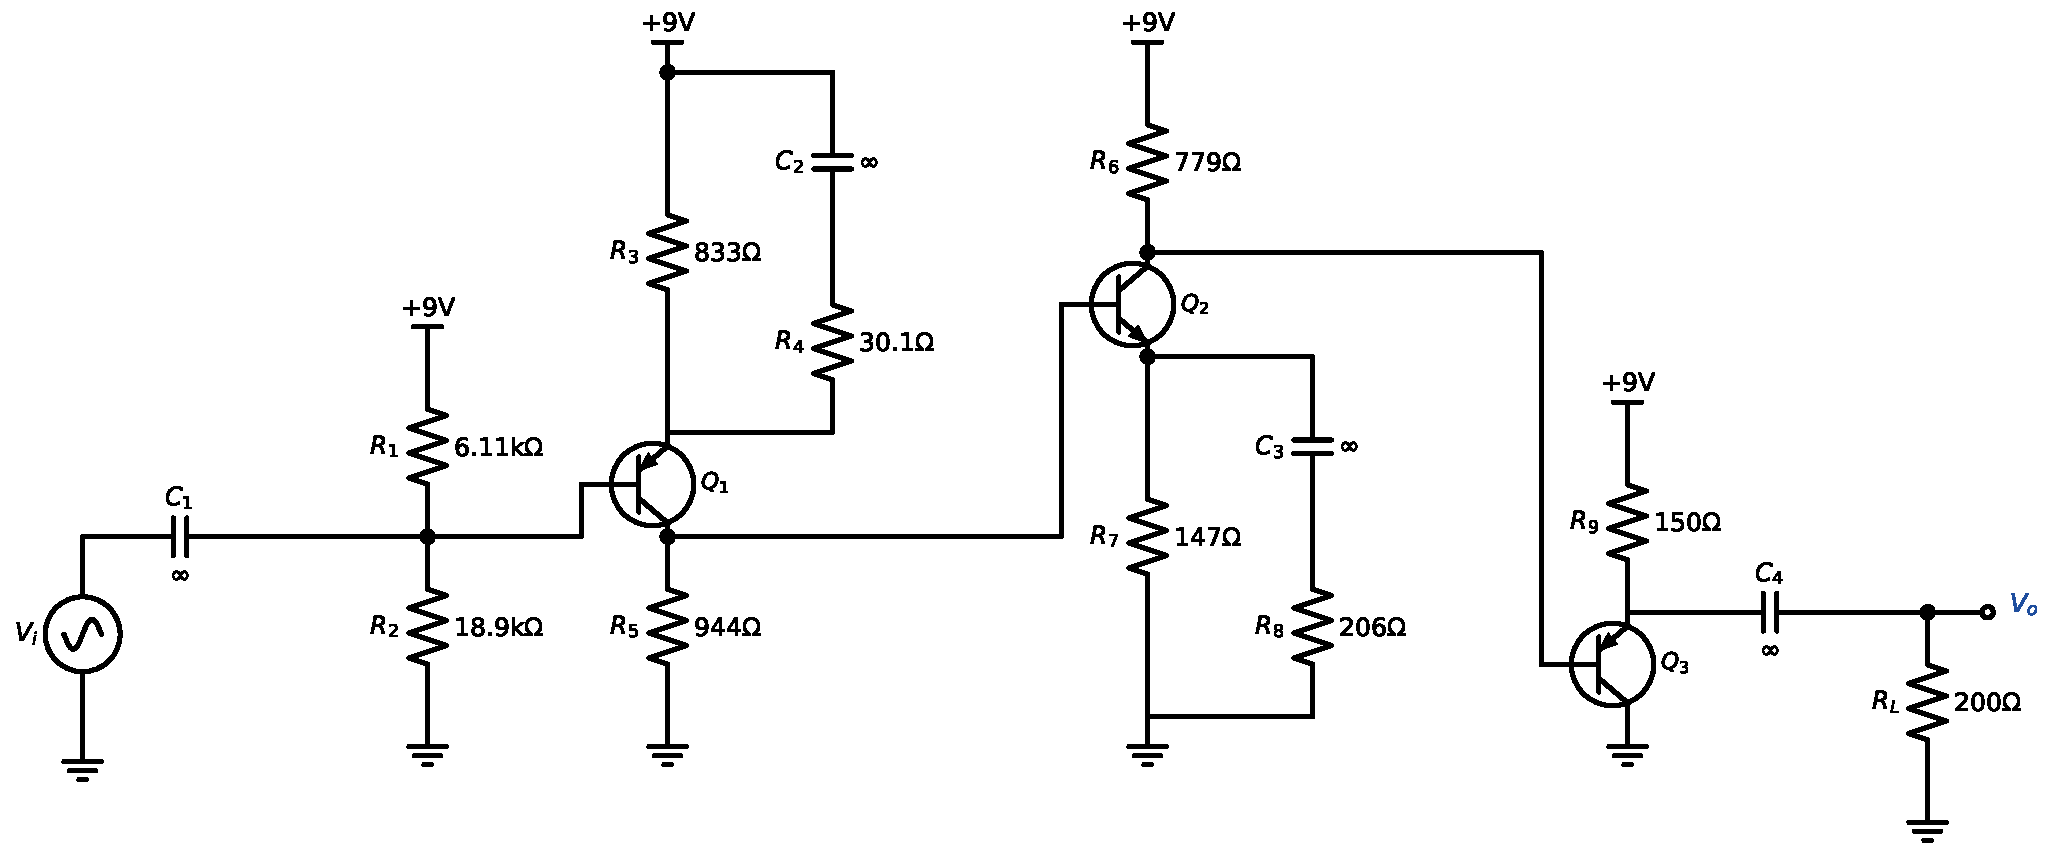
\includegraphics[width=0.9\linewidth,height=6.5cm,keepaspectratio]{p17_designed}\end{center}

\begin{ansbox}
$R_{1} = 6.11\,\mathrm{k}\Omega$,\quad $R_{2} = 18.9\,\mathrm{k}\Omega$,\quad $R_{3} = 833\,\Omega$,\quad $R_{4} = 30.1\,\Omega$,\quad $R_{5} = 944\,\Omega$,\quad $R_{6} = 779\,\Omega$,\quad $R_{7} = 147\,\Omega$,\quad $R_{8} = 206\,\Omega$,\quad $R_{9} = 150\,\Omega$
\end{ansbox}

\newpage
\subsection*{Solution 4E.18 \hfill Hard}
\begin{center}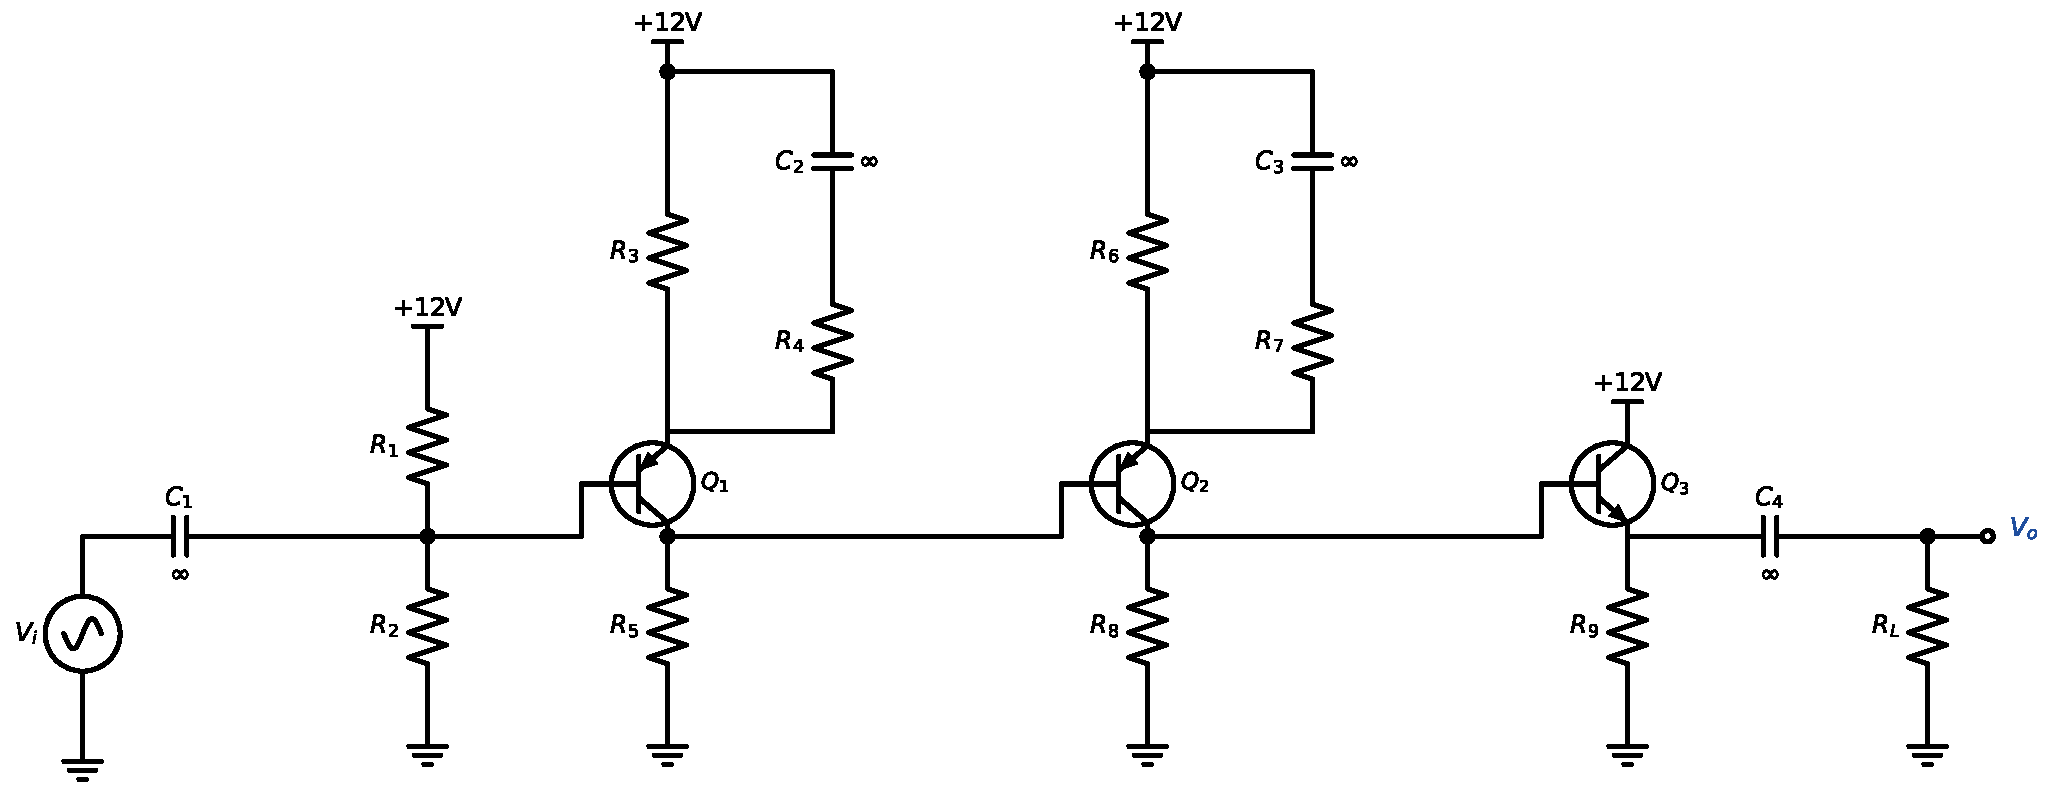
\includegraphics[width=0.9\linewidth,height=6cm,keepaspectratio]{p18_circuit}\end{center}
\solstep{1}{Plan}Name the resistors by their job: $R_{1} = R_{B1}$, $R_{2} = R_{B2}$, $R_{3} = R_{E1}$, $R_{4} = R_{G1}$, $R_{5} = R_{C1}$, $R_{6} = R_{E2}$, $R_{7} = R_{G2}$, $R_{8} = R_{C2}$, $R_{9} = R_H$. Every stage is biased like the one-stage design of the slides: $V_{RE}\ge1$\,V ($V_{BE}$-insensitive), the divider and every collector current much larger than the base current it feeds ($\beta$-insensitive, factor $N$), and $V_{RC}$ as large as the swing allows. Small-signal tools: $r_e = V_T/I_C$, CE gain $|A_v| = \frac{Z_C}{r_e + R_E\|R_G}$, follower gain $\frac{Z_E}{r_e+Z_E}$, base resistance $(\beta+1)(r_e + Z_E)$ (the $\infty$ capacitors put $R_G$ in parallel with $R_E$ for AC only). Design from the output back to the input, because each stage loads the one before it.
\solstep{2}{Output stage and follower}$V_{BE}$-insensitive: $V_{RE2} \ge 1$\,V; use $V_{RE2} = 1$\,V.

Collector swing of $Q_{2}$: about $\hat V_o$ (the follower has a gain close to 1). Largest $V_{RC2}$ without clipping: \[V_{RC2} = V_{CC} - \hat V_o - V_{RE2} - V_{CE,sat} = 12 - 3.5 - 1 - 0.2 = 7.3\,\mathrm{V}\]

Follower $Q_{3}$: its emitter sits at $0.7$\,V from the collector of $Q_{2}$, so $V_{RH} = V_{RC2} - 0.7 = 6.6\,\mathrm{V}$. To avoid current clipping the DC current in $R_H$ must stay larger than the peak current pushed into $R_L$: \[\frac{V_{RC2} - 0.7 - \hat V_o}{R_H} \ge \frac{\hat V_o}{R_L} \Rightarrow R_H \le R_L\frac{V_{RC2} - 0.7 - \hat V_o}{\hat V_o} = 1\,\mathrm{k}\Omega\cdot\frac{6.6 - 3.5}{3.5} = 886\,\Omega\]Take the E12 value just below: $R_H = \mathbf{820\,\Omega}$. Then $I_{C3} \approx \frac{V_{RH}}{R_H} = \frac{6.6}{820\,\Omega} = 8.05\,\mathrm{m}\mathrm{A}$, $r_{e3} = \frac{V_T}{I_{C3}} = 3.11\,\Omega$, and with $R_H \| R_L = 451\,\Omega$:\[A_{v3} = \frac{R_H\|R_L}{r_{e3} + R_H\|R_L} = 0.9932,\qquad R_{i3} = (\beta+1)(r_{e3} + R_H\|R_L) = 45.8\,\mathrm{k}\Omega\]
\solstep{3}{Stage 2 (common emitter, $Q_{2}$)}$\beta$-insensitive: $I_{C2} \ge N\frac{I_{C3}}{\beta} = 10\cdot\frac{8.05\,\mathrm{m}\mathrm{A}}{100} = 805\,\mu \mathrm{A}$; take the E12 value just above, $I_{C2} = 820\,\mu \mathrm{A}$.

\[R_{C2} = \frac{V_{RC2}}{I_{C2}} = \frac{7.3}{820\,\mu \mathrm{A}} = \mathbf{8.9\,\mathrm{k}\Omega},\quad R_{E2} = \frac{V_{RE2}}{I_{C2}} = \frac{1}{820\,\mu \mathrm{A}} = \mathbf{1.22\,\mathrm{k}\Omega},\quad r_{e2} = \frac{V_T}{I_{C2}} = 30.5\,\Omega\]

Gain $|A_{v2}| = \frac{R_{C2}\|R_{i3}}{r_{e2} + R_{E2}\|R_{G2}} = 12$ with $R_{C2}\|R_{i3} = 7.45\,\mathrm{k}\Omega$:\[R_{E2}\|R_{G2} = \frac{R_{C2}\|R_{i3}}{|A_{v2}|} - r_{e2} = 591\,\Omega \;\Rightarrow\; R_{G2} = \frac{1}{\frac{1}{591\,\Omega} - \frac{1}{1.22\,\mathrm{k}\Omega}} = \mathbf{1.15\,\mathrm{k}\Omega}\]

Its input resistance: $R_{i2} = (\beta+1)(r_{e2} + R_{E2}\|R_{G2}) = 62.7\,\mathrm{k}\Omega$.
\solstep{4}{Input stage ($Q_1$)}Gain left for stage 1: $|A_{v1}| = \frac{|A_v|}{|A_{v2}| A_{v3}} = \frac{300}{11.92} = 25.17$. The base of $Q_2$ fixes the collector of $Q_1$: $V_{RC1} = 10.3\,\mathrm{V}$. Its collector swing is only $\hat V_o/(\text{gain after it}) = 0.2937\,\mathrm{V}$, so $V_{RE1} \le V_{CC} - V_{RC1} - V_{CE,sat} - 0.294 = 1.206\,\mathrm{V}$; with $V_{RE1} \ge 1$\,V use $V_{RE1} = 1$\,V.

Divider: $V_{RB2} = V_{B1} = 10.3\,\mathrm{V}$, $V_{RB1} = V_{CC} - V_{B1} = 1.7\,\mathrm{V}$ ($|V_{RE1}| + 0.7$ on the emitter side). $\beta$-insensitive: the divider current is $N$ times the base current, $I_{RB} = N\frac{I_{C1}}{\beta}$, $N = 10$. Input resistance (all three in parallel, with $(\beta+1)(r_e + R_E\|R_G) \approx \beta\frac{R_{C1}}{|A_{v1}|} = \beta\frac{V_{RC1}}{I_{C1}|A_{v1}|}$):\[R_i \approx \frac{\beta/I_{C1}}{\frac{N}{V_{RB1}} + \frac{N}{V_{RB2}} + \frac{|A_{v1}|}{V_{RC1}}} \ge R_{i,spec} \;\Rightarrow\; I_{C1} \le \frac{\beta/R_{i,spec}}{\frac{10}{1.7} + \frac{10}{10.3} + \frac{25.17}{10.3}} = 5.38\,\mathrm{m}\mathrm{A}\]Take the E12 value just below: $I_{C1} = 4.7\,\mathrm{m}\mathrm{A}$. 

Check $I_{C1} \ge N\frac{I_{C2}}{\beta} = 82\,\mu \mathrm{A}$ \checkmark. 

\[R_{C1} = \frac{V_{RC1}}{I_{C1}} = \frac{10.3}{4.7\,\mathrm{m}\mathrm{A}} = \mathbf{2.19\,\mathrm{k}\Omega},\quad R_{E1} = \frac{V_{RE1}}{I_{C1}} = \frac{1}{4.7\,\mathrm{m}\mathrm{A}} = \mathbf{213\,\Omega},\quad r_{e1} = \frac{V_T}{I_{C1}} = 5.32\,\Omega\]

Gain $|A_{v1}| = \frac{R_{C1}\|R_{i2}}{r_{e1} + R_{E1}\|R_{G1}} = 25.17$ with $R_{C1}\|R_{i2} = 2.12\,\mathrm{k}\Omega$:\[R_{E1}\|R_{G1} = \frac{R_{C1}\|R_{i2}}{|A_{v1}|} - r_{e1} = 78.8\,\Omega \;\Rightarrow\; R_{G1} = \frac{1}{\frac{1}{78.8\,\Omega} - \frac{1}{213\,\Omega}} = \mathbf{125\,\Omega}\]

\[R_{B1} = \frac{V_{RB1}}{N I_{C1}/\beta} = \frac{1.7}{470\,\mu \mathrm{A}} = \mathbf{3.62\,\mathrm{k}\Omega},\qquad R_{B2} = \frac{V_{RB2}}{N I_{C1}/\beta} = \frac{10.3}{470\,\mu \mathrm{A}} = \mathbf{21.9\,\mathrm{k}\Omega}\]

Check: $R_i = R_{B1}\|R_{B2}\|(\beta+1)(r_{e1} + R_{E1}\|R_{G1}) = 3.62\,\mathrm{k}\Omega\|21.9\,\mathrm{k}\Omega\|8.5\,\mathrm{k}\Omega = 2.274\,\mathrm{k}\Omega$ $\ge 2\,\mathrm{k}\Omega$ \checkmark.
\solstep{5}{Check by analysis}Solve the finished circuit exactly ($\beta=100$, base currents included) for the DC point, then the small-signal gain with the exact $r_e$ values:\begin{center}\renewcommand{\arraystretch}{1.35}
\begin{tabular}{cccc}
\toprule
 & design $I_C$ & exact $I_C$ & exact $|V_{CE}|$ \\
\midrule
$Q_{1}$ & $4.7\,\mathrm{m}\mathrm{A}$ & $4.07\,\mathrm{m}\mathrm{A}$ & $2.174\,\mathrm{V}$ \\
$Q_{2}$ & $820\,\mu \mathrm{A}$ & $1.91\,\mathrm{m}\mathrm{A}$ & $5.736\,\mathrm{V}$ \\
$Q_{3}$ & $8.05\,\mathrm{m}\mathrm{A}$ & $17.7\,\mathrm{m}\mathrm{A}$ & $2.689\,\mathrm{V}$ \\
\bottomrule
\end{tabular}\end{center}
The exact currents are a little off the design values: $N$ only makes each base current $N$ times smaller than the current it disturbs, so the base voltages sag slightly, and along direct-coupled stages each shift is passed on (and amplified) to the next stage. The slides handle this the same way: simulate, then adjust. The exact gain is $|A_v| = 300.2$, within $0.5\,\%$ of the specification \checkmark. \begin{itemize}[leftmargin=*,itemsep=2pt]
\item Input resistance (exact): $R_i = 2.28\,\mathrm{k}\Omega$ $\ge 2\,\mathrm{k}\Omega$ \checkmark
\item Output swing: follower current clipping at $\hat V_o = I_{E3}(R_H\|R_L) = 7.991\,\mathrm{V}$; $Q_{2}$ clips (saturation or cutoff) at $\hat V_o = 5.519\,\mathrm{V}$; $Q_{1}$ clips (saturation or cutoff) at $\hat V_o = 24.04\,\mathrm{V}$. The smallest, $5.519\,\mathrm{V}$, is $\ge 3$\,V \checkmark
\item Distortion: each CE stage adds $HD_2 \approx \frac{\hat v_b}{4V_T}\left(\frac{r_e}{r_e + R_E\|R_G}\right)^2$ ($\hat v_b$ = its input amplitude at the specified output; for one stage this is the slides' $\frac{\hat V_o V_T |A_v|}{4V_{RC}^2}$): THD $\approx 0.052 + 0.12\,\% = 0.17\,\%$ $\le 5\,\%$ \checkmark
\item $V_{BE}$-insensitive: $V_{RE1} = 1$\,V, $V_{RE2} = 1$\,V $\ge 1$\,V \checkmark
\end{itemize}

\begin{center}\renewcommand{\arraystretch}{1.35}
\begin{tabular}{ll}
\toprule
resistor & value \\
\midrule
$R_{1}$ ($R_{B1}$) & $3.62\,\mathrm{k}\Omega$ \\
$R_{2}$ ($R_{B2}$) & $21.9\,\mathrm{k}\Omega$ \\
$R_{3}$ ($R_{E1}$) & $213\,\Omega$ \\
$R_{4}$ ($R_{G1}$) & $125\,\Omega$ \\
$R_{5}$ ($R_{C1}$) & $2.19\,\mathrm{k}\Omega$ \\
$R_{6}$ ($R_{E2}$) & $1.22\,\mathrm{k}\Omega$ \\
$R_{7}$ ($R_{G2}$) & $1.15\,\mathrm{k}\Omega$ \\
$R_{8}$ ($R_{C2}$) & $8.9\,\mathrm{k}\Omega$ \\
$R_{9}$ ($R_H$) & $820\,\Omega$ \\
\bottomrule
\end{tabular}\end{center}
\begin{center}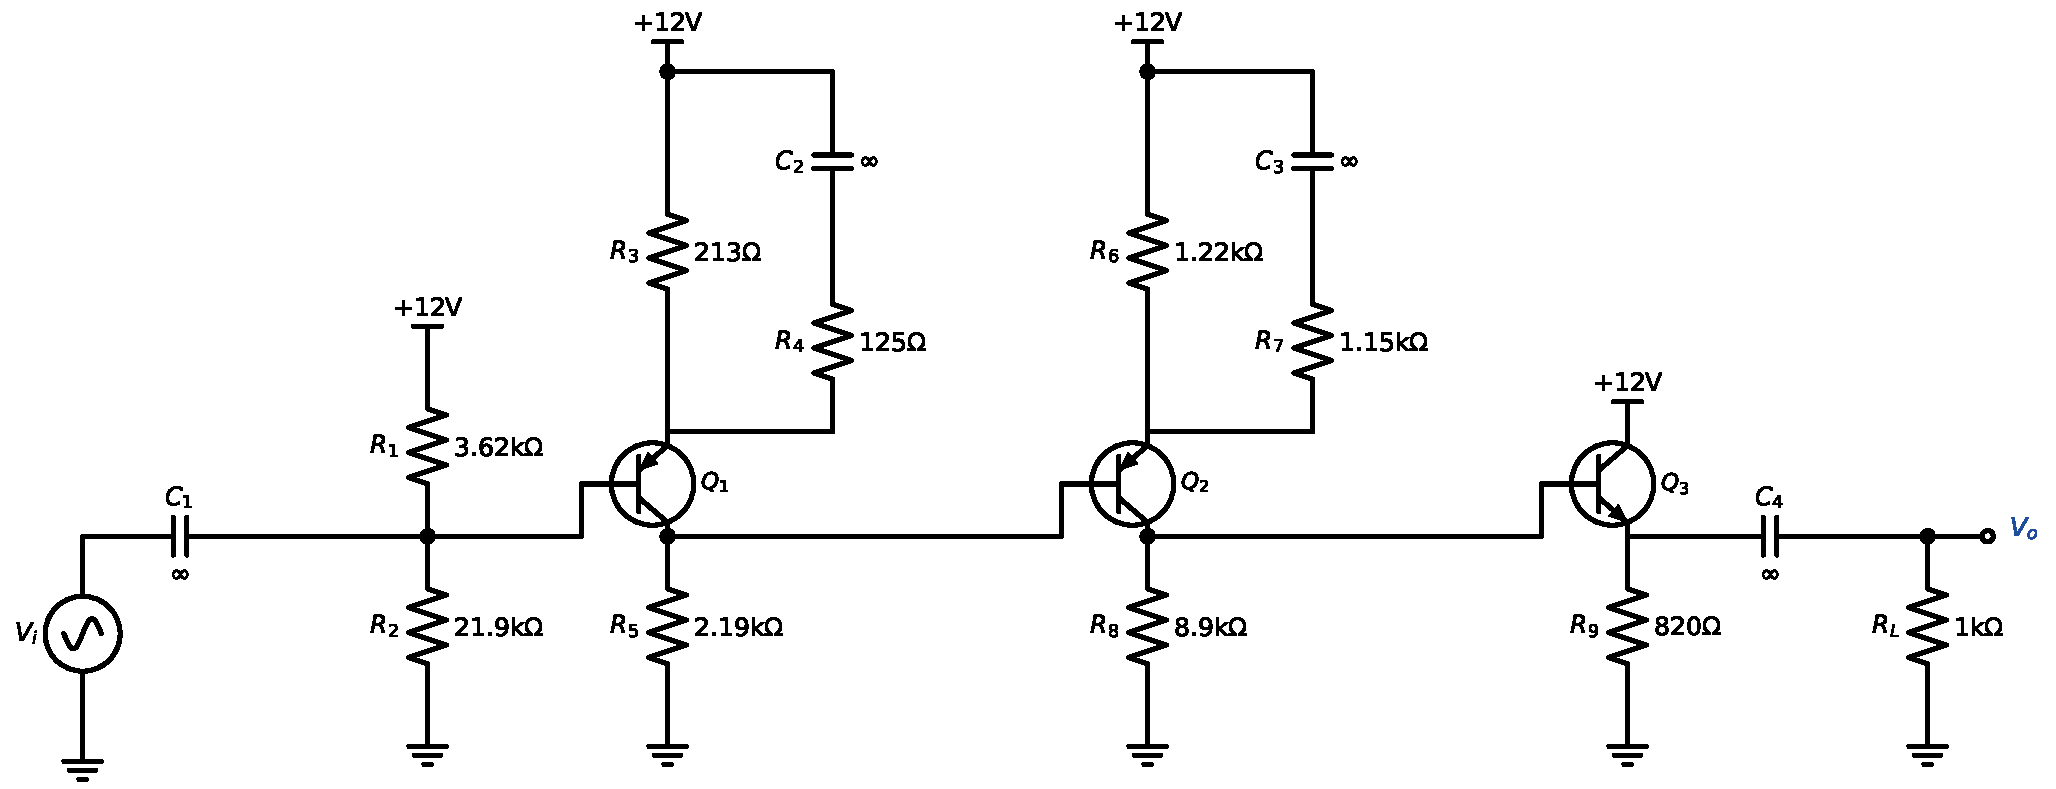
\includegraphics[width=0.9\linewidth,height=6.5cm,keepaspectratio]{p18_designed}\end{center}

\begin{ansbox}
$R_{1} = 3.62\,\mathrm{k}\Omega$,\quad $R_{2} = 21.9\,\mathrm{k}\Omega$,\quad $R_{3} = 213\,\Omega$,\quad $R_{4} = 125\,\Omega$,\quad $R_{5} = 2.19\,\mathrm{k}\Omega$,\quad $R_{6} = 1.22\,\mathrm{k}\Omega$,\quad $R_{7} = 1.15\,\mathrm{k}\Omega$,\quad $R_{8} = 8.9\,\mathrm{k}\Omega$,\quad $R_{9} = 820\,\Omega$
\end{ansbox}

\end{document}
